%-------------------------------------------------------------------------------
% This file provides a skeleton ATLAS paper.
%-------------------------------------------------------------------------------
% \pdfoutput=1
% The \pdfoutput command is needed by arXiv/JHEP/JINST to ensure use of pdflatex.
% It should be included in the first 5 lines of the file.
% \pdfinclusioncopyfonts=1
% This command may be needed in order to get \ell in PDF plots to appear. Found in
% https://tex.stackexchange.com/questions/322010/pdflatex-glyph-undefined-symbols-disappear-from-included-pdf
%-------------------------------------------------------------------------------
% Specify where ATLAS LaTeX style files can be found.
\newcommand*{\ATLASLATEXPATH}{latex/}
% Use this variant if the files are in a central location, e.g. $HOME/texmf.
% \newcommand*{\ATLASLATEXPATH}{}
%-------------------------------------------------------------------------------
\documentclass[PAPER, atlasdraft=true, texlive=2016, UKenglish, coverpage, PAPER]{\ATLASLATEXPATH atlasdoc}
% The language of the document must be set: usually UKenglish or USenglish.
% british and american also work!
% Commonly used options:
%  atlasdraft=true|false This document is an ATLAS draft.
%  texlive=YYYY          Specify TeX Live version (2016 is default).
%  coverpage             Create ATLAS draft cover page for collaboration circulation.
%                        See atlas-draft-cover.tex for a list of variables that should be defined.
%  cernpreprint          Create front page for a CERN preprint.
%                        See atlas-preprint-cover.tex for a list of variables that should be defined.
%  NOTE                  The document is an ATLAS note (draft).
%  PAPER                 The document is an ATLAS paper (draft).
%  CONF                  The document is a CONF note (draft).
%  PUB                   The document is a PUB note (draft).
%  BOOK                  The document is of book form, like an LOI or TDR (draft)
%  txfonts=true|false    Use txfonts rather than the default newtx
%  paper=a4|letter       Set paper size to A4 (default) or letter.

%-------------------------------------------------------------------------------
% Extra packages:
\usepackage[backend=bibtex]{\ATLASLATEXPATH atlaspackage}
% Commonly used options:
%  biblatex=true|false   Use biblatex (default) or bibtex for the bibliography.
%  backend=bibtex        Use the bibtex backend rather than biber.
%  subfigure|subfig|subcaption  to use one of these packages for figures in figures.
%  minimal               Minimal set of packages.
%  default               Standard set of packages.
%  full                  Full set of packages.
%-------------------------------------------------------------------------------
% Style file with biblatex options for ATLAS documents.
\usepackage{\ATLASLATEXPATH atlasbiblatex}

% Useful macros
\usepackage{\ATLASLATEXPATH atlasphysics}
\usepackage{multirow}
\newcommand{\DeltaP}{$\Delta_P(\rvar)$}
\newcommand{\DeltaTheta}{$\Delta_\Theta(\rvar)$}
\newcommand{\RP}{$R_P(\rvar)$}
\newcommand{\RTheta}{$R_\Theta(\rvar)$}
\newcommand{\DeltaDptr}{\mbox{$\Delta\Dptr$}}
\newcommand{\Dptr}{\mbox{$D( \pT, r)$}}
\newcommand{\RDptr}{\mbox{$R_{D( \pT, r)}$}}
\newcommand{\nucnuc}{\mbox{A+A}}
\newcommand{\AuAu}{\mbox{Au+Au}}
\newcommand{\PbPb}{\mbox{Pb+Pb}}
\newcommand{\pbpb}{\mbox{Pb+Pb}}
%\newcommand{\pp}{\mbox{$pp$}}
\newcommand{\dR}{\mbox{$\Delta R$}}

\newcommand{\pTmin}{\mbox{$p_{\mathrm{T,min}}$}}
\newcommand{\pTmax}{\mbox{$p_{\mathrm{T,max}}$}}
\newcommand{\dpT}{\mbox{$\mathrm{d}p_{\mathrm{T}}$}}
\newcommand{\NBJ}{\mbox{$R_{\Delta R}$}}
\newcommand{\Et}{\mbox{$E_{\mathrm{T}}$}}
%\newcommand{\ET}{\mbox{$E_{\mathrm{T}}$}}
%\newcommand{\pt}{\mbox{$p_{\mathrm{T}}$}}
%\newcommand{\pT}{\mbox{$p_{\mathrm{T}}$}}
\newcommand{\RNBJ}{\mbox{$\rho_{R_{\Delta R}}$}}
\newcommand{\ETtest}{\mbox{$E_{\mathrm{T}}^\mathrm{test}$}}
\newcommand{\ETnbj}{\mbox{$E_{\mathrm{T}}^\mathrm{nbr}$}}
\newcommand{\ETcombi}{\mbox{$E_{\mathrm{T}}^\mathrm{comb}$}}
\newcommand{\ETmerged}{\mbox{$E_{\mathrm{T}}^\mathrm{merged}$}}

\newcommand{\ANpart}{\mbox{$\langle N_{\mathrm{part}}\rangle$}}
\newcommand{\Ncoll}{\mbox{$N_{\mathrm{coll}}$}}
%\newcommand{\Nevt}{\mbox{$N_{\mathrm{evt}}$}}
\newcommand{\Ncone}{\mbox{$N_{\mathrm{cone}}$}}
\newcommand{\Njetcent}{\mbox{$N_{\mathrm{jet}}^{\mathrm{cent}}$}}
\newcommand{\Njet}{\mbox{$N_{\mathrm{jet}}$}}
\newcommand{\Nch}{\mbox{$n_{\mathrm{ch}}$}}
\newcommand{\NchUE}{\mbox{$N_{\mathrm{ch}}^{\mathrm{UE}}$}}
\newcommand{\nchUE}{\mbox{$n_{\mathrm{ch}}^{\mathrm{UE}}$}}
\newcommand{\nchmeas}{\mbox{$n_{\mathrm{ch}}^{\mathrm{meas}}$}}
\newcommand{\nchsub}{\mbox{$n_{\mathrm{ch}}^{\mathrm{sub}}$}}
\newcommand{\nchunf}{\mbox{$n_{\mathrm{ch}}^{\mathrm{unfolded}}$}}
\newcommand{\nch}{\mbox{$n_{\mathrm{ch}}$}}
\newcommand{\Npart}{\mbox{$N_{\mathrm{part}}$}}
\newcommand{\Ntptrt}{N_{\mathrm{2p}}}
\newcommand{\Ntptr}{\mbox{$N_{\mathrm{2p}}$}}
\newcommand{\Nraw}{\mbox{$N^{\mathrm{raw}}$}}
\newcommand{\sqrtsnn}{\mbox{$\sqrt{s_{_\text{NN}}}$}}
%\newcommand*{\sqn}{\ensuremath{\sqrt{s_{_\text{NN}}}}\xspace}
\newcommand{\sqrts}{\mbox{$\sqrt{s}$}}
\newcommand{\centrm}{\mathrm{cent}}
\newcommand{\pythia}{{\textsc PYTHIA}}
\newcommand{\pythiasix}{{\textsc Pythia}6}
\newcommand{\pythiaeight}{\textsc{Pythia}8}
\newcommand{\herwig}{{\textsc Herwig++}}
\newcommand{\powheg}{\textsc{Powheg}}


\newcommand{\RAA}{\mbox{$R_{\rm AA}$}}
\newcommand{\RFive}{\mbox{$R = 0.5$}}
\newcommand{\RFour}{\mbox{$R = 0.4$}}
\newcommand{\RThree}{\mbox{$R = 0.3$}}
\newcommand{\RTwo}{\mbox{$R= 0.2$}}
\newcommand{\Rcp}{\mbox{$R_{\rm CP}$}}
\newcommand{\Rpc}{\mbox{$R_{\rm PC}$}}
\newcommand{\Sk}{\mbox{$S(k)$}}
\newcommand{\TAA}{\mbox{$T_{\mathrm{AA}}$}}

%\newcommand{\antikt}{\mbox{anti-\kt}}
\newcommand{\avgpttrue}{\mbox{$\langle p_{\mathrm{T}}^{\mathrm{truth}}\rangle$}}
\newcommand{\centup}{^{\mathrm{cent}}}
\newcommand{\deffrel}{\mbox{$\delta \varepsilon/\varepsilon$}}
\newcommand{\ETfcal}{\mbox{$\Sigma E_{\mathrm{T}}^{\mathrm{FCal}}$}}
\newcommand{\eff}{\mbox{$\varepsilon$}}
\newcommand{\ETtruth}{\mbox{$E_{\mathrm{T}}^{\mathrm{truth}}$}}
\newcommand{\fs}{\mbox{${f_{\mathrm{S}}}$}}
\newcommand{\gjet}{\mbox{$\gamma$-jet}}
\newcommand{\invnb}{\mbox{${\rm nb^{-1}}$}}
%\newcommand{\kt}{\mbox{$k_{t}$}}
\newcommand{\sumet}{\mbox{$\Sigma E_{\mathrm{T}}$}}
\newcommand{\ETrec}{\mbox{$E_{\mathrm{T}}^{\mathrm{rec}}$}}
\newcommand{\ETtbyf}{\mbox{$E_{\mathrm{T}}^{3\times 4}$}}
\newcommand{\ETsbys}{\mbox{$E_{\mathrm{T}}^{7\times 7}$}}
\newcommand{\Dphi}{\mbox{$\Delta \phi$}}
\newcommand{\Deta}{\mbox{$\Delta \eta$}}
\newcommand{\DpT}{\mbox{$\Delta \pT$}}
\newcommand{\Dz}{\mbox{$D(z)$}}
\newcommand{\Dzmeas}{\mbox{$D^{\mathrm{meas}}(z)$}}
\newcommand{\Dzsub}{\mbox{$D^{\mathrm{sub}}(z)$}}
\newcommand{\Dpt}{\mbox{$D(\pT)$}}
\newcommand{\Dptmeas}{\mbox{$D^{\mathrm{meas}}(\pT)$}}
\newcommand{\Dptsub}{\mbox{$D^{\mathrm{sub}}(\pttrk)$}}
\newcommand{\Dptratio}{\mbox{$D(\pT)|_{\mathrm{cent}}/D(\pT)|_{\mathrm{60-80}}$}}
\newcommand{\Dzratio}{\mbox{$D(z)|_{\mathrm{cent}}/D(z)|_{\mathrm{60-80}}$}}
\newcommand{\Delpt}{\mbox{$\Delta \pT$}}
\newcommand{\DRtrk}{\mbox{$\Delta R_{\mathrm{trk}}$}}
\newcommand{\effpteta}{\mbox{$\varepsilon(\pT, \eta)$}}
\newcommand{\effpt}{\mbox{$\varepsilon(\pT)$}}
\newcommand{\phat}{\mbox{$\hat{p}_{\mathrm{T}}$}}
\newcommand{\pthatmin}{\mbox{$\hat{p}^{\mathrm{min}}_{\mathrm{T}}$}}
\newcommand{\pthat}{\mbox{$\hat{p}_{\mathrm{T}}$}}
\newcommand{\etajet}{\mbox{$\eta^{\mathrm{jet}}$}}
\newcommand{\phijet}{\mbox{$\phi^{\mathrm{jet}}$}}
\newcommand{\pTjet}{\mbox{$p_{{\mathrm{T}}}$}}
\newcommand{\pTjetcorr}{\mbox{$p_{{\mathrm{T}}}^{\mathrm{corr}}$}}
\newcommand{\pTch}{\mbox{$p_{{\mathrm{T}}}^{\mathrm{ch}}$}}
\newcommand{\pTtrk}{\mbox{$p_{{\mathrm{T}}}^{\mathrm{ch}}$}}
\newcommand{\pttrk}{\mbox{$p_{\mathrm{T}}^{\mathrm{ch}}$}}
%\newcommand{\pttrk}{\mbox{$p_{\mathrm{T}}^{\mathrm{trk}}$}}
%\newcommand{\pTtrk}{\mbox{$p_{{\mathrm{T}}}^{\mathrm{trk}}$}}
\newcommand{\pTrec}{\mbox{$p_{{\mathrm{T}}}^{\mathrm{rec}}$}}
\newcommand{\pTtrue}{\mbox{$p_{\mathrm{T}}^{\mathrm{truth}}$}}
\newcommand{\etatrue}{\mbox{$\eta^{\mathrm{truth}}$}}
\newcommand{\ztrue}{\mbox{$z^{\mathrm{truth}}$}}
\newcommand{\zrec}{\mbox{$z^{\mathrm{rec}}$}}
\newcommand{\ptvjet}{\mbox{$\displaystyle {\vec{p}_{\mathrm{T}}}^{\, \mathrm{jet}}$}}
\newcommand{\ptvchg}{\mbox{$\displaystyle {\vec{p}_{\mathrm{T}}}^{\, \mathrm{chg}}$}}
\newcommand{\ntrue}{\mbox{$N^{\mathrm{truth}}$}}
\newcommand{\nmatch}{\mbox{$N^{\mathrm{match}}$}}
\newcommand{\rcpcorr}{\mbox{$R_{\mathrm{CP}}$}}
\newcommand{\rcpraw}{\mbox{$R_{\mathrm{CP}}^{\mathrm{meas}}$}}
\newcommand{\unfdn}{_{\mathrm{unf}}}
\newcommand{\xini}{\mbox{$x_{\mathrm{ini}}$}}
\newcommand{\vtjet}{\mbox{$v_2^{\mathrm{jet}}$}}
\newcommand{\vtjetmeas}{\mbox{${v_2^{\mathrm{jet}}|_{\mathrm{meas}}}$}}
\newcommand{\vtwo}{\mbox{$v_2$}}
\newcommand{\Rdz}{\mbox{$R_{D(z)}$}}
\newcommand{\Rdpt}{\mbox{$R_{D(\pT)}$}}
\newcommand{\Rdzsub}{\mbox{$R_{D(z)}^{\mathrm{sub}}$}}
\newcommand{\Rdptsub}{\mbox{$R_{D(\pT)}^{\mathrm{sub}}$}}
\newcommand{\Psit}{\mbox{$\Psi_2$}}

\newcommand{\Psires}{\mbox{$\mathrm{Res}\{\Psi_2\}$}}
\newcommand{\Rpsi}{\mbox{$R_{\Delta \phi}$}}
\newcommand{\diff}{\mathrm{d}}
\newcommand{\dpsi}{\mbox{$\Delta\phi$}}
\newcommand{\dNdpTdpsi}{\mbox{$\diff^2\Njet/\diff\pt\diff\dpsi$}}
\newcommand{\dNdpTdpsiRaw}{\mbox{$\dfrac{\diff^2N_{\mathrm{jet}}^{\mathrm{raw}}}{\diff\pt\diff\dpsi}$}}
\newcommand{\dNdpTdpsiCorr}{\mbox{$\dfrac{\diff^2N_{\mathrm{jet}}^{\mathrm{corr}}}{\diff\pt\diff\dpsi}$}}

\newcommand{\ETjet}{\mbox{$\ET^{\mathrm{jet}}$}}
\newcommand{\pbarp}{\mbox{$p+\bar{p}$}}
\newcommand{\pPb}{\mbox{$p$+Pb}}
%\newcommand{\pt}{\mbox{$p_T$}}
\newcommand{\ptjet}{\mbox{$p_{\mathrm{T}}^{\mathrm{jet}}$}}
%\newcommand{\pt}{\mbox{$p_{\mathrm{T}}$}}
%\newcommand{\etatrk}{\mbox{$\eta^{\mathrm{trk}}$}}
\newcommand{\etatrk}{\mbox{$\eta^{\mathrm{ch}}$}}
\newcommand{\ptpart}{\mbox{$p_{\mathrm{T}}^{\mathrm{part}}$}}
\newcommand{\pttruth}{\mbox{$p_{\mathrm{T}}^{\mathrm{reco}}$}}
\newcommand{\ptreco}{\mbox{$p_{\mathrm{T}}^{\mathrm{truth}}$}}
%\newcommand{\etapart}{\mbox{$\eta^{part}$}}
\newcommand{\ystar}{\mbox{$y^{*}_{\mathrm{jet}}$}}
\newcommand{\yjet}{\mbox{$y^{\mathrm{jet}}$}}
\newcommand{\Lres}{\mbox{$L_{\mathrm{res}}$}}
\newcommand{\Rres}{\mbox{$R_{\mathrm{res}}$}}
\newcommand{\dndeta}{\mbox{$1/\Nevt \, d\Nch/d\eta$}}
\newcommand{\RpPb}{\mbox{$R_{p\mathrm{Pb}}$}}
\newcommand{\Jt}{\mbox{$j_{\mathrm{T}}$}}
\newcommand{\jt}{\mbox{$j_{\mathrm{T}}$}}
\newcommand{\xt}{\mbox{$x_{\mathrm{T}}$}}
\newcommand{\ETtrue}{\mbox{$E_{\mathrm{T}}^{\mathrm{truth}}$}}
\newcommand{\ETreco}{\mbox{$E_{\mathrm{T}}^{\mathrm{reco}}$}}
\newcommand{\RSix}{\mbox{$R= 0.6$}}
\newcommand{\EffJet}{\mbox{$\varepsilon_{\mathrm{jet}}$}}
\newcommand{\Aj}{\mbox{$A_{\mathrm{J}}$}}
\newcommand{\dphi}{$\Delta \phi$}
\newcommand{\p}{\partial}
\newcommand{\rvar}{\mbox{$r$}}
\renewcommand{\_}{{\tt \char`\_}}  % works properly only in \tt mode (!)
\newcommand{\z}{\mbox{$z$}}
\newcommand{\zunfolded}{\mbox{$z_{\mathrm{unfolded}}$}}
\newcommand{\zreco}{\mbox{$z_{\mathrm{reco}}$}}
\newcommand{\ztruth}{\mbox{$z_{\mathrm{truth}}$}}
\newcommand{\Rdzmeas}{\mbox{$R_{D(z)}^{\mathrm{meas}}$}}
\newcommand{\Rdptmeas}{\mbox{$R_{D(\pT)}^{\mathrm{meas}}$}}
\newcommand{\ptjettruth}{\mbox{$p_{{\mathrm{T}}}^{\mathrm{jet,truth}}$}}
\newcommand{\ptjetreco}{\mbox{$p_{{\mathrm{T}}}^{\mathrm{jet,reco}}$}}
\newcommand{\ptjetunfolded}{\mbox{$p_{{\mathrm{T}}}^{\mathrm{jet,unfolded}}$}}
\newcommand{\fd}{\mathrm{d}}
\newcommand{\cnchUE}{\mbox{$\tilde{n}_{\mathrm{ch}}^{\mathrm{UE+fake}}$}}

%\newcommand{\Dzunf}{\mbox{$D^{\mathrm{unfolded}}(z)$}}
%\newcommand{\Dptunf}{\mbox{$D^{\mathrm{unfolded}}(\pT)$}}
\newcommand{\Dzunf}{\mbox{$\frac{\diff\Nch}{\diff z}$}}
\newcommand{\Dptunf}{\mbox{$\frac{\diff\Nch}{\diff \pt}$}}



% See doc/atlas_physics.pdf for a list of the defined symbols.
% Default options are:
%   true:  journal, misc, particle, unit, xref
%   false: BSM, heppparticle, hepprocess, hion, jetetmiss, math, process,
%          other, snippets, texmf
% See the package for details on the options.

% Files with references for use with biblatex.
% Note that biber gives an error if it finds empty bib files.
 \addbibresource{trkjet.bib}
\addbibresource{bib/ATLAS.bib}
\addbibresource{bib/CMS.bib}
\addbibresource{bib/ConfNotes.bib}
\addbibresource{bib/PubNotes.bib}

% Paths for figures - do not forget the / at the end of the directory name.
\graphicspath{{logos/}{figures/}}

% Add you own definitions here (file trkjet-defs.sty).
\usepackage{trkjet-defs}
\usepackage[utf8]{inputenc}

%-------------------------------------------------------------------------------
% Generic document information
%-------------------------------------------------------------------------------

% Title, abstract and document 
% !TEX root = trkjet.tex
%-------------------------------------------------------------------------------
% This file contains the title, author and abstract.
% It also contains all relevant document numbers used by the different cover pages.
%-------------------------------------------------------------------------------

% Title
\AtlasTitle{Measurement of angular and momentum distributions of charged particles within and around jets in \pbpb\ and $pp$ collisions at $\sqrt{s_{\mathrm{NN}}}=$~5.02~\TeV\ with ATLAS at the LHC}

% Draft version:
% Should be 1.0 for the first circulation, and 2.0 for the second circulation.
% If given, adds draft version on front page, a 'DRAFT' box on top of each other page, 
% and line numbers.
% Comment or remove in final version.
\AtlasVersion{0.14}

% Abstract - % directly after { is important for correct indentation
\AtlasAbstract{%
Studies of the fragmentation of jets into charged particles in heavy-ion collisions can provide information
about
 the mechanism of jet quenching by the hot and dense QCD matter created in such collisions, the quark-gluon plasma. 
This paper presents a measurement of the angular distribution of charged particles around the jet axis in $\sqrt{s_{\mathrm{NN}}}=$~5.02~\TeV\
 Pb+Pb and \textit{pp} collisions, done using the ATLAS detector at the LHC. The measurement is performed for jets reconstructed with the \antikt\ algorithm with radius parameter $R = $~0.4, and is extended to a distance of $r= 0.8$ from the jet axis. The charged particles used in this analysis have transverse momenta in the \mbox{1--63 GeV} range and are within an absolute value of pseudorapidity of 2.5. They are associated to jets with an absolute value of jet rapidity of less than 1.7, and transverse momenta in the \mbox{126--316 GeV} range. Results are presented as a function of Pb+Pb collision centrality and distance from the jet axis for different jet and charged-particle transverse momenta ranges. The previously observed enhancement of charged particles with transverse momenta below 4 GeV is measured to increase for larger angular distances from the jet axis achieving a maximum at $r=0.6$. Charged particles with transverse momenta above 4 GeV show an enhancement in Pb+Pb collisions only in the jet core for distances up to $r = 0.05$ and a suppression at all larger distances from the jet axis.
}

% Author - this does not work with revtex (add it after \begin{document})
% This has to be commented out for TDR etc.
 \author{The ATLAS Collaboration}

% ATLAS reference code, to help ATLAS members to locate the paper
\AtlasRefCode{ANA-HION-2018-03-PAPER}

% CERN preprint number
% \PreprintIdNumber{CERN-EP-2019-XX}

% ATLAS date - arXiv submission; usually filled in by the Physics Office
 \AtlasDate{\today}

% ATLAS heading - heading at top of title page. Set for TDR etc.
% \AtlasHeading{ATLAS ABC TDR}

% arXiv identifier
% \arXivId{14XX.YYYY}

% HepData record
% \HepDataRecord{ZZZZZZZZ}

% Submission journal and final reference
 \AtlasJournal{Phys.\ Rev.\ C.}
% \AtlasJournalRef{\PLB 789 (2017) 123}
% \AtlasDOI{}

%-------------------------------------------------------------------------------
% The following information is needed for the cover page. The commands are only defined
% if you use the coverpage option in atlasdoc or use the atlascover package
%-------------------------------------------------------------------------------

% List of supporting notes  (leave as null \AtlasCoverSupportingNote{} if you want to skip this option)
 \AtlasCoverSupportingNote{Correlations between jets and charged particles in Pb+Pb Collisions at 5.02 TeV}{https://cds.cern.ch/record/2304504}
% \AtlasCoverSupportingNote{Short title note 2}{https://cds.cern.ch/record/YYYYYYY}
%
% OR (the 2nd option is deprecated, especially for CONF and PUB notes)
%
% Supporting material TWiki page  (leave as null \AtlasCoverTwikiURL{} if you want to skip this option)
% \AtlasCoverTwikiURL{https://twiki.cern.ch/twiki/bin/view/Atlas/WebHome}

% Comment deadline
% \AtlasCoverCommentsDeadline{DD Month 2019}

% Analysis team members - contact editors should no longer be specified
% as there is a generic email list name for the editors
 \AtlasCoverAnalysisTeam{Akshat Puri, Anne Sickles, Martin Rybar}

% Editorial Board Members - indicate the Chair by a (chair) after his/her name
% Give either all members at once (then they appear on one line), or separately
 \AtlasCoverEdBoardMember{Mario Martinez Perez(chair), Iwona Grabowska-Bold, Benjamin Nachman}
% \AtlasCoverEdBoardMember{EdBoard~Chair~(chair)}
% \AtlasCoverEdBoardMember{EB~Member~1}
% \AtlasCoverEdBoardMember{EB~Member~2}
% \AtlasCoverEdBoardMember{EB~Member~3}

% A PUB note has readers and not an EdBoard--give their names here (one line or several entries)
% \AtlasCoverReaderMember{Reader~1, Reader~2}
% \AtlasCoverReaderMember{Reader~1}
% \AtlasCoverEdBoardMember{Reader~2}

% Editors egroup
 \AtlasCoverEgroupEditors{atlas-ana-hion-2018-03-analysis-team@cern.ch}

% EdBoard egroup
 \AtlasCoverEgroupEdBoard{atlas-ana-hion-2018-03-editorial-board@cern.ch}

% Author and title for the PDF file
\hypersetup{pdftitle={ATLAS document},pdfauthor={The ATLAS Collaboration}}

%-------------------------------------------------------------------------------
% Content
%-------------------------------------------------------------------------------
\begin{document}

\maketitle

\tableofcontents

%-------------------------------------------------------------------------------
\section{Introduction}
\label{sec:intro}
% !TEX root = trkjet.tex

Ultra-relativistic nuclear collisions at the Large Hadron Collider (LHC) produce hot, dense matter called the quark-gluon plasma, QGP (see Refs.~\cite{Roland:2014jsa,Busza:2018rrf} for recent reviews).
Jets from hard-scattering processes in these collisions traverse and interact with the QGP, losing energy via a process called jet-quenching.
The rates and characteristics of these jets in heavy-ion collisions can be compared to the same quantities in \pp\ collisions, where we do not expect the production of QGP.
This comparison can provide information on the properties of the QGP and how it interacts with partons from the hard scatter.

Jets with large transverse momenta in central lead-lead (\pbpb) collisions at the LHC are measured at approximately half the rates in \pp\ collisions when the nuclear overlap function of \pbpb\ collisions is taken into account~\cite{Abelev:2013kqa,Aad:2014bxa,Adam:2015ewa,Khachatryan:2016jfl, 2019108}.
Similarly, back-to-back dijet~\cite{Aad:2010bu,Chatrchyan:2011sx,Aaboud:2017eww} and photon-jet pairs~\cite{Chatrchyan:2012gt,Aaboud:2018anc} are observed to have less balanced transverse momenta in \pbpb\ collisions compared to \pp\ collisions.
These observations suggest that some of the energy from the hard-scattered parton may be transferred outside of the jet through its interaction with the QGP medium.
 
Complementary measurements look at how the structure of jets is different between \pbpb\ and \pp\ collisions.
Jet shape measurements in the \pp\ and \pbpb\ collision systems have shown a broadening of the jets due to the QGP~\cite{Aad:2011sc, Acharya:2018uvf, Chatrchyan:2012mec, Chatrchyan:2013kwa}.
Additionally, measurements of longitudinal fragmentation functions at the LHC show an excess, in PbPb collisions, of low and high momentum particles with a depletion of intermediate momentum particles inside the jet compared to pp collisions~\cite{Aad:2014wha,Chatrchyan:2014ava,Aaboud:2017bzv,Aaboud:2018hpb}.
Particles carrying a large fraction of the jet momentum are generally closely aligned with the jet axis, whereas low momentum particles are observed to have a much broader angular distribution extending outside the jet~\cite{Chatrchyan:2011sx,Khachatryan:2015lha,Khachatryan:2016tfj,Sirunyan:2018jqr}.
These observations suggest that the energy lost via jet-quenching is being transferred to soft particles around the jet axis via soft gluon emission~\cite{Vitev:2008rz,Ovanesyan:2011xy,Blaizot:2014ula,Qin:2015srf,Escobedo:2016jbm,Casalderrey-Solana:2016jvj,Tachibana:2017syd}.
Measurements of yields of these particles as a function of transverse momentum and angular distance between the particle and the jet axis have a potential to provide further insight into on the structure of jets in the QGP, as well as provide information on how the medium is affected by the presence of the jet.


This paper presents charged-particle \pt\ distributions around the jet axis that have been corrected for detector effects.
The measured yields are defined as:

\begin{align*}
\Dptr = \frac{1}{N_{\mathrm{jet}}} \frac{1}{A} \frac{\mathrm{d} n_{\mathrm{ch}} (\pt, r)}{\mathrm{d} \pt},
%%%
%D(\pt,\ptjet) = \frac{1}{N_{\mathrm{jet}}} ~ \frac{1}{\epsilon(\pttrk)} ~ \frac{\mathrm{d} N_{\mathrm{ch}}}{\mathrm{d} \pt}~(\ptjet).
%%%
\end{align*}
where $r = \sqrt{\Delta \eta^2 + \Delta \phi^2}$ \footnote{ATLAS uses a right-handed coordinate system with its origin at the nominal interaction point (IP) in the centre of the detector, and the $z$-axis along the beam pipe.
The $x$-axis points from the IP to the centre of the LHC ring, and the $y$-axis points upward.
Cylindrical coordinates $(r,\phi)$ are used in the transverse plane, $\phi$ being the azimuthal angle around the $z$-axis.
The pseudorapidity is defined in terms of the polar angle $\theta$ as $\eta=-\ln\tan(\theta/2)$.
The rapidity is defined as $y = 0.5\text{ln}[(E + p_z)/(E-p_z)]$ where $E$ and $p_z$ are the energy and $z$-component of the momentum along the beam direction respectively.
Transverse momentum and transverse energy are defined as $\pt = p \sin\theta$ and $\Et = E \sin\theta$, respectively.
The angular distance between two objects with relative differences $\Delta \eta$ and $\Delta \phi$ in pseudorapidity and azimuth respectively is given by $\sqrt{(\Delta \eta )^2 + (\Delta \phi)^2}$.} 
is the angular distance from the jet axis and $N_{\mathrm{jet}}$ is the number of jets in consideration.
$A = \pi (r_{\mathrm{max}}^2 - r_{\mathrm{min}}^2) $ is the area of an annulus around the jet axis with its inner and outer radii $r_{\mathrm{min}}$ and $r_{\mathrm{max}}$ respectively and $n_{\mathrm{ch}}(\pt, r)$ is the number of charged particles with a given \pt\ within the annulus.
The ratios of the charged-particle yields measured in \pbpb\ and \pp\ collisions,

\begin{align*}
   \RDptr = \frac{\Dptr_\mathrm{Pb+Pb}}{\Dptr_{\pp}},
\end{align*}
quantify the modifications of the yields due to the QGP medium.
Furthermore, the differences between the \Dptr\ distributions in \pbpb\ and \pp\ collisions, 

\begin{align*}
   \Delta \Dptr = \Dptr_\mathrm{Pb+Pb} - \Dptr_{pp},
\end{align*}
allow for measuring the absolute differences in charged-particle yields between the two collision systems.



%The analysis is done using 0.49~nb$^{-1}$ of \pbpb\ collisions and 
%25~pb$^{-1}$ of \pp\ collisions at center-of-mass energy of 5.02~\TeV\ collected in 2015 by ATLAS.

%The \pbpb\ collisions are divided into the following centrality intervals: 0--10\%, 10--20\%, 20--30\%, 30--40\%, 40--60\%, 60--80\%.
%It uses jets reconstructed with the \antikt\ algorithm \cite{Cacciari:2008qp} using a radius parameter of \RFour, restricted to the rapidity interval of $|\yjet| <$~1.7 and having transverse momenta \ptjet\ in the 126--316 GeV range.
%Charged particles associated with these jets are restricted to $|\eta| < 2.5$ and have a transverse momenta of $\pt > 1$ GeV.
%The measurement is done in annuli at increasing distances from the jet axis.
%These annuli have their inner and outer radius $r_{\textrm{min}}$ and $r_{\textrm{max}}$ and take the following values: 0.0, 0.05, 0.1, 0.15, 0.2, 0.25, 0.3, 0.4, 0.5, 0.6, 0.7, 0.8.


%-------------------------------------------------------------------------------
%-------------------------------------------------------------------------------
\section{Experimental setup}
\label{sec:setup}
% !TEX root = trkjet.tex

The measurements presented here are performed using the ATLAS calorimeter, inner detector, trigger,
and data acquisition systems~\cite{Aad:2008zzm}. 
%The primary components used in the measurement of \Dptr\ distributions are the calorimeters and the inner detector.
The calorimeter system consists of a sampling liquid-argon (LAr) electromagnetic (EM) calorimeter covering $|\eta|<3.2$, a
steel--scintillator sampling hadronic calorimeter covering $|\eta| <1.7$, LAr hadronic calorimeters covering $1.5 < |\eta| < 3.2$, and
two LAr forward calorimeters~(FCal) covering $3.1 < |\eta| <
4.9$. 
% and has a $\Delta
%\eta \times \Delta \phi$ granularity of $0.1 \times
%0.1$ for $|\eta| < 2.5$ and  $0.2 \times 0.2$ for $2.5 < |\eta| < 4.9$.\footnote{An 
%  exception is the third sampling layer that has a segmentation of $0.2 \times 0.1$
%up to $|\eta| = 1.4$.}
The EM calorimeters are segmented longitudinally in shower depth into three
layers with an additional pre-sampler layer. They
have segmentation that varies with layer and pseudorapidity. 
The hadronic calorimeters have three sampling layers longitudinal
in shower depth.
%The EM calorimeters have a granularity that varies with layer and pseudorapidity, but which is generally much finer than that of the hadronic calorimeter.

The inner detector measures charged particles  within the pseudorapidity interval  $|\eta|<2.5$ using a combination of silicon pixel detectors, silicon microstrip detectors (SCT), and a straw-tube transition radiation tracker (TRT), all immersed in a 2~T axial magnetic field~\cite{Aad:2008zzm}. Each of the three detectors is composed of a barrel and two symmetric end-cap sections. The pixel detector is composed of four layers including the "insertable B-layer" (IBL)~\cite{ibl1,ibl2}. The SCT barrel section contains four layers of modules with sensors on both sides, and each end-cap consists of nine layers of double-sided modules with radial strips. The TRT contains layers of staggered straws interleaved with fibers in the barrel and end-cap.


%The inner detector measures charged particles  within the pseudorapidity interval  $|\eta|<2.5$ using a combination of silicon pixel detectors, silicon microstrip detectors (SCT), and a straw-tube transition radiation tracker (TRT), all immersed in a 2~T axial magnetic field~\cite{Aad:2008zzm}. Each of the three detectors is composed of a barrel and two symmetric end-cap sections. The pixel detector  is composed of four layers: the "insertable B-layer" (IBL)~\cite{ibl1,ibl2} and three layers  with a pixel size of $50~{ \mu \mathrm{m}} \, \times \, 400~{ \mu \mathrm{m}}$.  The  SCT barrel section contains four layers of modules with 80~$\mu {\mathrm m}$  pitch sensors on both sides and each end-cap consists of nine layers of double-sided modules with radial strips having a mean pitch of $80~\mathrm{\mu m}$. The two sides of each SCT layer in both the barrel and the end-caps have a relative stereo angle of 40~mrad. The TRT contains up to 73 (160) layers of staggered straws interleaved with fibres in the barrel (end-cap).

The zero-degree calorimeters (ZDCs) are located symmetrically at $z = \pm140$~m and cover $|\eta| > 8.3$.
The ZDCs use tungsten plates as absorbers, and quartz rods sandwiched between the tungsten plates as the active medium. In \PbPb\ collisions the ZDCs primarily measure ``spectator'' neutrons, that is neutrons that do not interact
hadronically when the incident nuclei collide. A ZDC coincidence trigger is implemented by requiring
the pulse height from both ZDCs to be above a threshold to accept the single-neutron peak.

A two-level trigger system is used to select the \PbPb\ and \pp\ collisions. The first level is based on custom electronics while the second level, the High Level Trigger (HLT), is based on software. 
%The first one, a hardware-based trigger stage Level-1, is implemented with custom electronics. The next level is the software-based High Level Trigger (HLT) and is used to further reduce the accepted event rate. 
Minimum-bias~(MB) events are recorded using trigger defined by a logical OR of following two triggers: 1) total energy Level-1 trigger; 2) veto on the total energy trigger and ZDC coincidence trigger at Level-1 with the additional requirement of least one track in the HLT. The total-energy trigger required a total transverse energy measured in the calorimeter system to be greater than 50~\GeV.  Jet events are selected by the HLT, seeded by a jet identified by the Level-1 jet trigger in \pp\ collisions or by the total-energy trigger with a threshold of 50~\GeV\ in \PbPb\ collisions. The Level-1 jet trigger utilized in \pp\ collisions required a jet with transverse momentum greater than 20~\GeV.
The HLT jet trigger used a jet reconstruction procedure similar to that used in the offline 
analysis as discussed in Section~\ref{sec:reconstruction}. 
It selected events containing jets with the transverse energy 
of at least 75~\GeV\ in \PbPb\ collisions and at least 
85~\GeV\ in \pp\ collisions. The measurement is performed in the 
jet transverse momentum range where the trigger is fully efficient.


%the minimum-bias trigger, with two total transverse-energy triggers requiring 1.5~\TeV\ and 6.5~\TeV\ being used to enhance the rate of more central \PbPb\ events.





%-------------------------------------------------------------------------------
\section{Data sets and event selection}
\label{sec:data}
% !TEX root = trkjet.tex

The \PbPb\ and \pp\ data used in this analysis were recorded in 2015.
 The data samples consist of 25~pb$^{-1}$ of \sqrts~=~5.02~\TeV\ \pp\ and 0.49~nb$^{-1}$ of \sqrtsnn~=~5.02~\TeV\
\pbpb\ data. In both samples, events are required to have a reconstructed vertex
within 150~mm of the nominal interaction point along the beam axis.
Only events taken during stable beam conditions and satisfying detector and data-quality requirements that include the calorimeters and inner tracking detectors being in nominal operating conditions are considered. 

%The MB
%\PbPb\ sample was recorded with different pre-scales\footnote{The pre-scale indicates which fraction of events that passed the trigger selection was selected for recording by the data  acquisition.}  depending on the instantaneous luminosity in the
%LHC fill. The MB trigger recorded an effective luminosity of 22 $\mu$b$^{-1}$.


In \PbPb\ collisions, the event centrality reflects the overlap area of the two colliding nuclei and is characterized by \ETfcal, the total transverse energy deposited in the 
FCal~\cite{Aaboud:2017tql}. The six centrality intervals used in this analysis are defined according to successive percentiles of the \ETfcal\ distribution obtained in minimum-bias collisions, ordered from the most central (highest \ETfcal) to the most peripheral (lowest \ETfcal) collisions: 0--10\%, 10--20\%, 20--30\%, 30--40\%, 40--60\%, 60--80\%. 

In addition to the jet-triggered sample, a separate minimum bias \PbPb\ data sample was recorded with three trigger selections: the minimum-bias trigger and two total transverse-energy triggers with thresholds of 1.5 TeV and 6.5 TeV used to enhance the rate of central \pbpb\ events. This sample was combined with a set of $1.8\times10^7$ 5.02 TeV hard-scattering dijet \pp\ events generated with \powheg{}+\pythiaeight\ \cite{Nason:2004rx,Sjostrand:2014zea} using the A14 tune of parameters \cite{ATLAS2014021} and the NNPDF23LO PDF set \cite{Ball:2012cx} to produce the Monte Carlo Overlay sample. This sample is reweighed on an event-by-event basis such that it has the same centrality distribution as the jet triggered sample.
A separate set of $1.8\times10^7$ 5.02 TeV hard-scattering dijet \pp\ events generated with the same tune and PDFs was used as the \pp\ MC. The detector response was simulated in both MC samples using \textsc{Geant4} \cite{Agostinelli:2002hh,Aad:2010ah} and was used to evaluate the performance of the detector and analysis procedure. Another sample of minimum bias \pbpb\ events was generated using HIJING (version 1.38b) \cite{Aad:2010ah} and was only used to evaluate the track reconstruction performance. 	


%A sample of 1.8~$\times10^{7}$ simulated 5.02~\TeV\ \powheg{}+\pythiaeight~\cite{Nason:2004rx,Sjostrand:2014zea} \pp\ hard-scattering events, generated using the A14 tune~\cite{ATLAS2014021} and the NNPDF23LO PDF set~\cite{Ball:2012cx}, is used to evaluate the performance for measuring \Dptr\ distributions in the \pp\ data. The performance of the detector and analysis procedure in \PbPb\ collisions is evaluated using 1.8~$\times10^{7}$ 5.02~\TeV\ hard-scattering dijet events generated with \powheg{}+\pythiaeight\ overlaid on top of events from the enhanced minimum-bias \PbPb\ data sample. In both samples, the detector response is simulated using \textsc{Geant}4~\cite{Agostinelli:2002hh,Aad:2010ah}. A weight is assigned to each MC event such that the event sample obtained from the simulation has the same \ETfcal\ distribution as in jet triggered data.



%-------------------------------------------------------------------------------
\section{Jet and track selection}
\label{sec:reconstruction}
% !TEX root = trkjet.tex

The jet reconstruction procedures closely follow those used by \mbox{ATLAS} for jet measurements in \pp\ and \PbPb\ collisions at
$\sqrtsnn=2.76$~\TeV~\cite{Aad:2014bxa} and 5.02 TeV \cite{2019108}.
The \antikt\ algorithm is first run in four-momentum recombination mode, on
$\Delta \eta \times \Delta \phi = 0.1\times 0.1$  calorimeter towers with two \antikt\ distance parameter values ($R=$~0.2 and $R=$~0.4). The energies in the towers are obtained by summing the
	energies of calorimeter cells at the electromagnetic energy scale within the tower boundaries. Then,
	  an iterative procedure is used to estimate the $\eta$-dependent underlying event (UE)  transverse energy density, while excluding the regions populated by jets. The estimate of the UE contribution is performed on an event-by-event basis.
	Furthermore, the background is modulated to account for the presence of the azimuthal anisotropy of particle production~\cite{ATLAS:2012at}. The modulation accounts for the contribution of the second, third, and fourth order azimuthal anisotropy harmonics.
	Higher order harmonics introduce a negligible variation of the reconstructed jet energy.
	The UE transverse energy is subtracted from calorimeter towers included in the jet and the four-momentum of the jet is updated accordingly.
	  Then, a jet $\eta$- and \pT-dependent  correction factor to the \ptjet\ 
	  derived from the simulation samples is applied to correct for the calorimeter energy
	  response~\cite{Aaboud:2017jcu}. The same calibration factors are applied both 
in \pp\ and \pbpb\ collisions.
An additional correction based on \textit{in-situ} studies of jets recoiling against photons, $Z$ bosons, and jets in other regions of the calorimeter is
	  applied~\cite{ATL-PHYS-PUB-2015-036,2019167}. The same jet reconstruction procedure without the
	  azimuthal modulation of the UE is also applied to $pp$ collisions.
	  In this analysis, jets are required to have \ptjet\ in the 126--316 \GeV\ range, with rapidity  $|\yjet|<$~1.7. 
 To prevent nearby jets from distorting the measurement of \Dptr\ distributions, 
jets are rejected if there is another jet with a higher \ptjet\ than the considered jet anywhere
within a distance of $\Delta R < 1.0$. The isolation requirement removes approximately 0.01\% of jets, and has almost no impact on the final measurement.

Charged-particle tracks are reconstructed from hits in the inner detector using the 
track reconstruction algorithm with settings optimized for the high hit density in heavy-ion
collisions~\cite{Aaboud:2017all}.
Tracks used in this analysis  are required to have at least 9 (11) total silicon hits for charged particles with pseudorapidity,  \mbox{|\etatrk| $\leq$ 1.65 (|\etatrk| > 1.65)}.  At least one hit is required in one of the two innermost pixel layers.
If the track trajectory passes through an active module in the innermost layer, then 
a hit in this layer is required. Additionally, a track must 
have no more than two holes in the pixel and SCT detectors together, where 
a hole is defined by the absence of a hit predicted by the track 
trajectory. 
All charged-particle tracks used in this analysis are required to have reconstructed transverse momentum $\pttrk > 1.6$~\GeV. In order to suppress a contribution from
secondary particles, the distance of closest approach of the track to the primary vertex is required to be less than a value which varies from  0.45~mm at $\pttrk=4$~\GeV\ to 0.2~mm at $\pttrk=20$~\GeV\ in the transverse plane and less than 1.0~mm in the longitudinal direction.


The efficiency, $\varepsilon(\pTtrue, \etatrue)$, for reconstructing charged particles in \PbPb\ and \pp\ collisions is evaluated as a function of the generator-level primary particle transverse momentum, \pTtrue, and pseudorapidity, \etatrue\, by matching tracks to generator-level primary particles\footnote{Primary particles are defined as particles with a mean lifetime $\tau>0.3\times 10^{-10}$s either directly produced in \pp\ interactions or from subsequent decays of particles with a shorter lifetime. All other particles are considered to be secondary.} using the MC samples described above~\cite{Aad:2010ah}. For \pbpb\ collisions, the efficiency is also evaluated separately in each centrality interval used in the measurement.
     
The contribution of reconstructed tracks that cannot be matched to a generated primary particle in the \pp\ MC samples, along with the residual contribution of tracks matched to secondary particles, are together called the contribution from ``fake'' tracks. This contribution is less than 2\% in the entire \pttrk\ range under study in both \pp\ and \pbpb\ collisions.  









%-------------------------------------------------------------------------------
\section{Analysis procedure}
\label{sec:analysis}
% !TEX root = trkjet.tex

The analysis procedure is similar to that in Ref.~\cite{Aaboud:2018hpb} with the additional requirement of being done differentially in \rvar. Measured tracks are associated with a reconstructed jet if they fall within $\Delta R < 0.8$ of the jet axis and are constructed as:

\begin{align*}
\dfrac{\fd^{2} \nchmeas }{ \fd \pttrk \fd r} = \frac{1}{\varepsilon(\pttrk,\etatrk)} \frac{\Delta \Nch( \pttrk, r)}{ \Delta\pttrk \Delta r}
\end{align*}

where $\Delta \Nch (\pttrk, r)$ represents the number of tracks within a given \pttrk\ and $r$ range. The efficiency correction is applied as a $1/\varepsilon(\pttrk,\etatrk)$ weight on a track-by-track basis, assuming $\pttrk = \pTtrue$. While that assumption is not strictly valid, the efficiency varies sufficiently slowly with $\pTtrue$ that the error
introduced by this assumption is less than 1\%. It is further corrected for by the Bayesian unfolding procedure described later in this section.

The measured track yields need to be corrected for the UE, fake tracks and secondaries. In \pp\ collisions, the UE contribution from hard scatterings not associated with jet production is negligible. The contributions from fake tracks and secondary charged particles are estimated from MC samples and subtracted. This procedure is similar to that applied in previous measurements~\cite{Aaboud:2017tke,Aaboud:2018hpb}.

For \pbpb\ collisions, the UE, fake track, and secondary contributions are estimated together in a two step process: first, MC overlay is used to generate \etajet--\phijet\ maps of the average number of charged particles in a given annulus around a reconstructed jet. This is done for charged particles without a truth match and as a function of \ptjet, \etajet, \phijet, angle of the jet to the second order event plane\footnote{The second order event plane angle $\Psi_2$ is determined on an event-by-event basis by a standard method using the $\phi$ variation of transverse energy in the FCal \cite{ATLAS:2012at}} $ \mathrm{d}\Psi_{\mathrm{jet}}$, \rvar, \pttrk, and centrality. In the second step, the \etajet--\phijet\ maps are used to generate the UE distribution for jets with a given \etajet, \phijet, and $\mathrm{d}\Psi_{\mathrm{jet}}$. This distribution includes fakes, and is given by \mbox{$\fd^2 \nch^{\mathrm{UE+Fake}}(\pttrk, r) / \fd \pttrk \fd r$}. The yields decrease with decreasing collision centrality, increasing \pttrk, and increasing azimuthal distance from $\Psi_2$. The subtracted distributions are then given by 

\begin{align*}
\frac{\fd^2 \nchsub }{ \fd \pttrk \fd r } &=  \frac{\fd^2 \nchmeas }{ \fd \pttrk \fd r} -  \frac{ \fd^2 \nch^{\mathrm{UE+Fake}}(r)  }{ \fd \pttrk \fd r} 
\end{align*}

Figure~\ref{fig:UEsize} shows the ratio of the charged-particle distributions before and after the subtraction of the UE, fake tracks, and secondaries,
%the charged-particle distributions prior to the UE and fake track subtraction, $ \fd^2 \nchmeas / \fd \pttrk \fd r$, divided by the distributions after the subtraction, $ \fd^2 \nchsub / \fd \pttrk \fd r $
 as a function of \rvar\ for different \pttrk\ intervals and $126 < \ptjet < 158$ \GeV\ for six centrality selections. The largest UE contribution is for 1.0~\GeV\ charged particles at large values of \rvar\ in central collisions, with the background being approximately 100 times the signal, and slowly decreasing with increasing \ptjet. It rapidly decreases for more peripheral collisions, larger \pttrk\ and smaller \rvar. In addition, due to the steeply falling nature of the jet \pt\ spectra, the smearing due to jet energy resolution leads to a net migration of jets from lower \ptjet\ to higher \ptjet\ values, such that a jet reconstructed with a given transverse momentum will correspond, on average, to a lower truth jet \pT.  This ``up-feeding'' induces a difference between the UE yields determined using the MC overlay events and the actual UE contribution to reconstructed jets. The magnitude of this difference is centrality dependent, and can be seen clearly for charged particles with $\pt > 10$ GeV.

\begin{figure}
\centerline{
 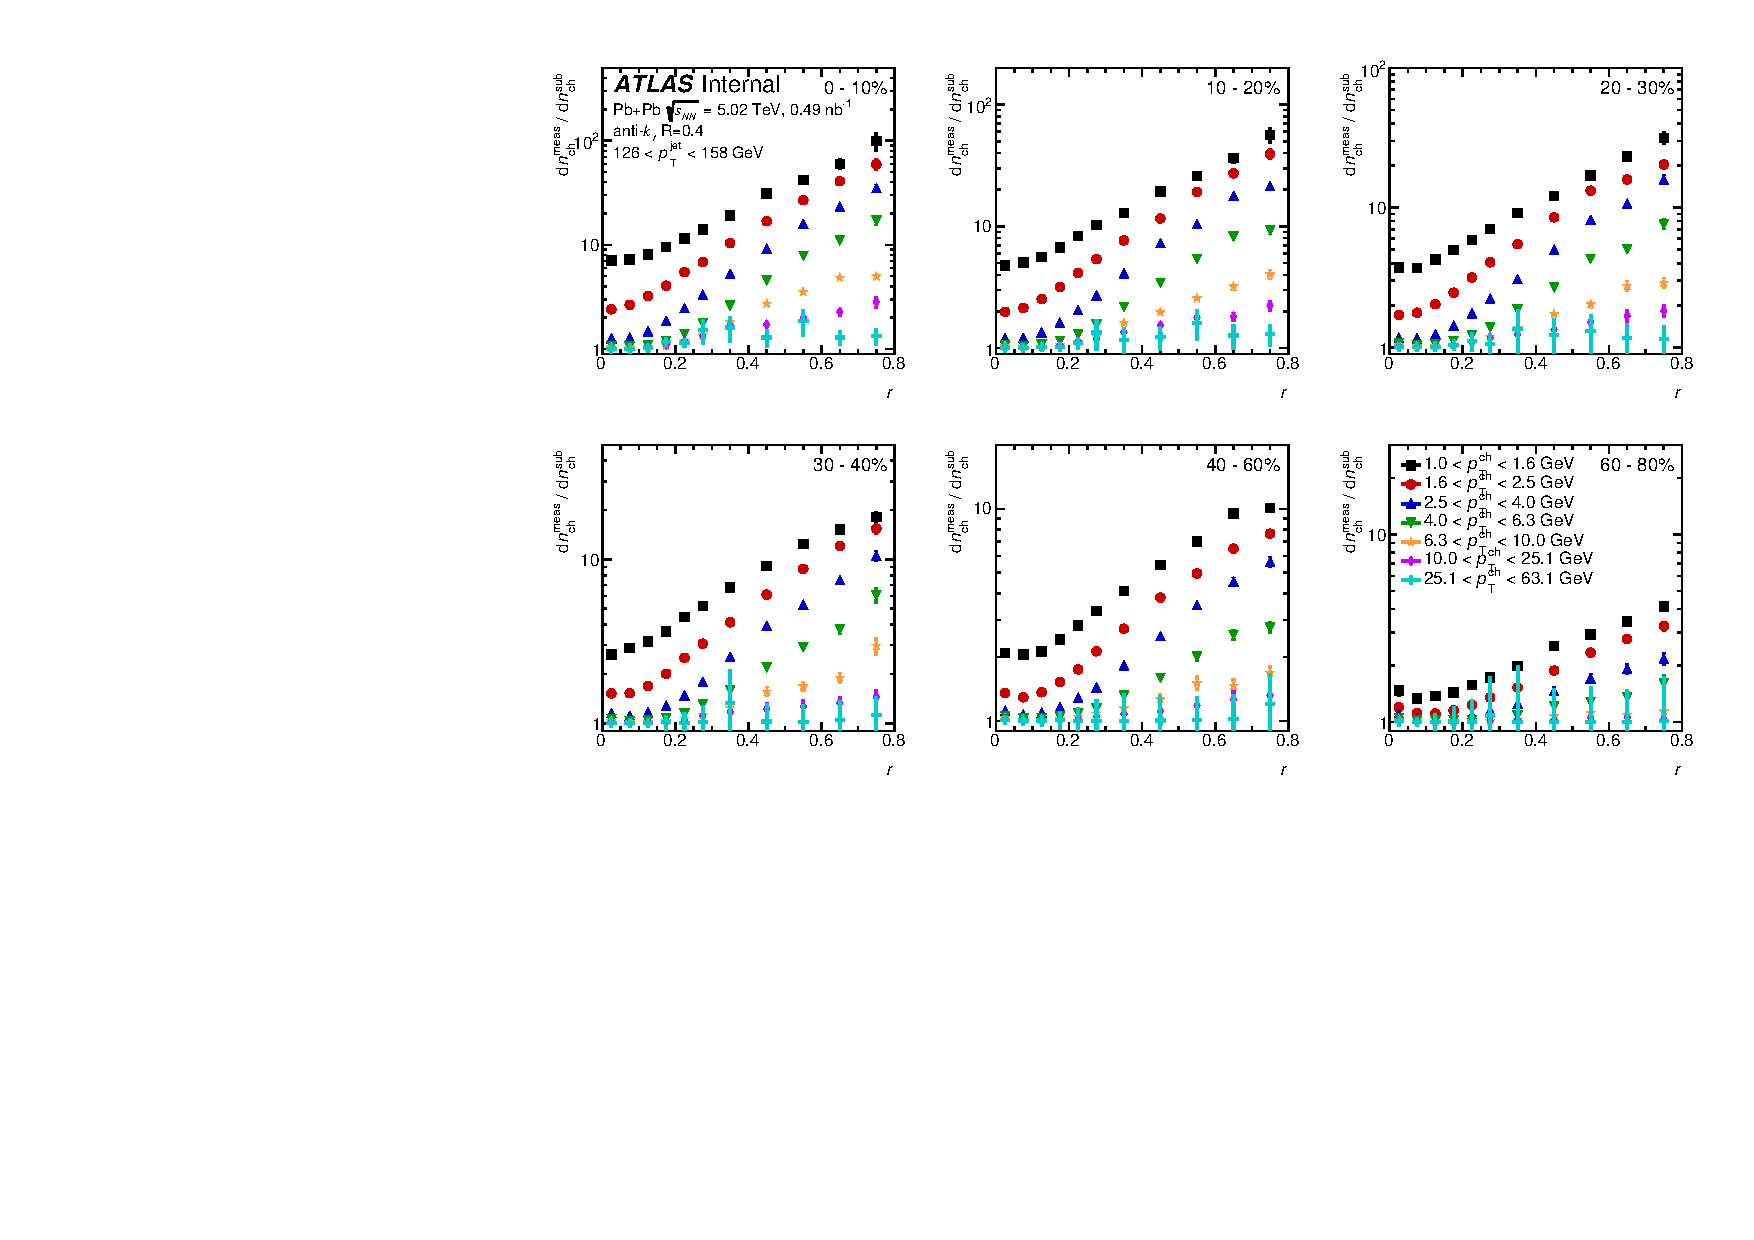
\includegraphics[width=0.95\textwidth]{figures/performance/UE_B2S_single_0.pdf} }
\caption{ Ratio of the raw charged particle distributions to those after the subtraction of the UE and fake tracks as a function of \rvar\ for different \pttrk\ intervals, six centrality selections and for \ptjet\ between 126--158~\GeV.}
\label{fig:UEsize}
\end{figure}


%The fraction of fake tracks is found to be below 2\% of the tracks that pass the selection in all track and jet kinematic regions in this analysis.

To remove the effects of the bin migration due to the jet energy and track momentum resolution, the subtracted $\fd^2 \nchsub /\fd\pttrk \fd r$ distributions are corrected by a two-dimensional Bayesian unfolding~\cite{DAgostini:1994zf}
in \pttrk\ and \ptjet\ as implemented in the RooUnfold package~\cite{Adye:2011gm}.  
Two-dimensional unfolding is used because the calorimetric jet energy response depends on the fragmentation pattern of the jet~\cite{Aad:2011he}.
Four-dimensional response matrices are created from the \pp\ and \pbpb\ MC samples using the generator-level and reconstructed \ptjet, and the generator-level and reconstructed charged-particle \pttrk. They are corrected for tracking efficiencies and are evaluated in bins of \rvar\ and centrality. The Bayesian procedure requires a choice in the number of iterations.
Additional iterations reduce the sensitivity to the choice of prior, but may
amplify statistical fluctuations in the distributions.
After four iterations the 
charged particle distributions are found to be stable for both the \PbPb\ and \pp\ data.
A separate one-dimensional Bayesian unfolding is used to correct the measured \ptjet\ spectra that are used to normalize the unfolded charged particle distributions.
To achieve better correspondence with the data, the response matrices for both the one and two dimensional unfolding are reweighed so that the charged particle and jet distributions match the shapes in the reconstructed data.

An independent bin-by-bin unfolding procedure is also used to correct for migrations originating from the finite jet and track angular resolutions. Two corresponding \Dptr\ distributions are evaluated in MC samples, one using \pythia\ jets and primary particles and the other using reconstructed jets and charged particles with their reconstructed \pt\ replaced by generator-level transverse momentum, \pTtrue. The ratio of these two MC distributions provides a correction factor which is then applied to the data. 

The final particle-level corrected distributions, normalized by the area of the annulus under question are defined as:

\begin{align*}
   \Dptr = \frac{1}{N_\mathrm{jet}^\mathrm{unfolded}} \frac{1}{A(r)} \frac{\fd^2 \nchunf(r)}{\fd \pt \fd r},
 \end{align*}
where $N_\mathrm{jet}^\mathrm{unfolded}$ is the unfolded number of jets in a given \ptjet\ interval, and \nchunf\  is the unfolded yield of charged particles with a given \pt in an annulus of area $A$ at a distance \rvar.

The performance of the full analysis procedure is validated in the MC samples by comparing the fully corrected charged particle distributions to the generator-level distributions. Good closure (< 4 \%) is seen for charged particles with $\pt < 10$ GeV in both the \pp\ and \pbpb\ collision systems. The non-closure is taken as an additional systematic uncertainty as discussed in Section~\ref{sec:systematics}.
It is to be noted that adding or removing particles carrying a large fraction of the jet momentum near the edge of the jet can significantly alter its
reconstructed momentum and position; this instability leads to some non-closure in the analysis procedure for particles with $\pt > 10$ GeV in jets with $\ptjet < 200$ GeV. 
Results are presented where the non-closure in the \pp\ MC sample is less than 5\%.

%, excluding the following regions of phase space: 6--10 GeV tracks above $\rvar > 0.3$, 10--25 GeV tracks above $\rvar > 0.3$, and 25--63 GeV tracks above $\rvar > 0.2$ for 126--158 GeV jets; 10--25 GeV tracks above $\rvar > 0.4$, and 25--63 GeV tracks above $\rvar > 0.3$ for 158--200 GeV jets; 25--63 GeV tracks above $\rvar > 0.3$ for 200--251 GeV jets.




%-------------------------------------------------------------------------------
\section{Systematic uncertainties}
\label{sec:systematics}
% !TEX root = trkjet.tex

The following sources of systematic uncertainty are considered:
the jet energy scale (JES), the jet energy resolution (JER), 
the sensitivity of the  unfolding to the prior, the UE contribution, the residual non-closure of the analysis procedure, and tracking-related uncertainties.
For each systematic variation, the \Dptr\ distributions along with their ratios and differences are re-evaluated. The difference between the varied and nominal distributions is used as an estimate of the uncertainty.

The systematic uncertainty due to the JES in \PbPb\ collisions is due to jets having a different structure and possibly a different detector response that is not modeled by the MC. It is composed of two parts: 
a centrality-independent baseline component and a centrality-dependent component. Only the centrality-independent baseline component is used in \pp\ collisions; 
it is determined from \textit{in-situ} studies of the calorimeter
response~\cite{Aad:2011he,HIjesnote,Aaboud:2017jcu} and the relative energy scale difference between the jet reconstruction procedures in heavy-ion~\cite{HIjesnote} and \pp\ collisions~\cite{Aad:2014bia}. The centrality-dependent uncertainty reflects a modification of parton showers by the \PbPb\ environment. It is evaluated by comparing calorimeter \ptjet\ and the sum of the transverse momentum of charged particles within the jet in data and MC. The size of the centrality-dependent uncertainty on the JES reaches 0.5\% in the most central collisions. Each component that contributes to the JES uncertainty is varied separately by $\pm1$ standard deviation for each interval in \ptjet\ and the response matrix is recomputed accordingly. The data are then unfolded with the modified matrices. The resulting uncertainty from the JES increases with increasing charged-particle \pT\ at fixed \ptjet\ and decreases with increasing \ptjet, and is at the level of 2--4\%.

The uncertainty on the \Dptr\ distributions due to the JER is evaluated by repeating the unfolding procedure with modified response matrices, where an additional contribution is added to the resolution of the reconstructed \ptjet\ using a Gaussian smearing procedure. The smearing factor is evaluated using an \textit{in-situ} technique in 13~\TeV\ \pp\ data that involves studies of dijet energy balance~\cite{Aad:2012ag,JERConfNote}. An additional uncertainty is included to account for differences between the tower-based jet reconstruction and that used in analyses of 13~\TeV\ \pp\ data. The resulting uncertainty from the JER is symmetrized to account for negative variations of the JER.  The size of the resulting uncertainty on the \Dptr\ distributions due to the JER typically reaches 4--5\% for the highest charged-particle \pT\ intervals and decreases to 2--3\% with decreasing charged-particle \pT\ at fixed \ptjet.


The uncertainties related to track reconstruction and selection originate from several sources.
Uncertainties related to the material description in simulation and the track transverse 
momentum resolution are obtained from studies in data and simulation described in Ref.~\cite{ATL-PHYS-PUB-2015-051}.
The sensitivity of the tracking efficiency to the description of the 
inactive material in the MC samples is evaluated by varying the material description.
This resulting uncertainty in the track reconstruction efficiency is between
0.5\% and 2\% in the track \pT\ range used in the analysis. 
The systematic uncertainty on the fakes and secondaries is 30\% in both collision systems~\cite{ATL-PHYS-PUB-2015-051}.  The contamination of fake tracks is less than 2\% and the resulting uncertainty in the \Dptr\ distributions is at most 5\%.
An additional uncertainty takes into account a possible residual misalignment of the tracking detectors
in \pp\ and \PbPb\ data-taking. The alignment in these datasets is checked \textit{in-situ} with $Z\rightarrow \mu^{+}\mu^{-}$ events, and the track-\pT\-dependent uncertainty arises from the finite size of this sample. The resulting uncertainties in
the \Dptr\ distributions are typically less than 0.1\%. An additional  uncertainty in the tracking efficiency due to the high local track density in the core of jets is 0.4\%~\cite{ATL-PHYS-PUB-2016-007} for all \ptjet\ ranges in this analysis. The uncertainty due to the track selection is evaluated by repeating the analysis with an additional requirement on the significance of the distance of closest approach of the track to the primary vertex. This uncertainty affects 
the track reconstruction efficiencies, track momentum resolution, and rate of fake tracks. The resulting uncertainty typically varies between 1--2\%.
Finally, the track-to-particle association requirements are varied. This variation affects the track reconstruction efficiency, track momentum resolution, and rate of fake tracks. The resulting systematic uncertainty is $\leq~0.1 \%$ on the \Dptr\ distributions. All track-related systematic uncertainties are added in quadrature and presented as the total tracking uncertainty. 

The systematic uncertainty associated with the UE subtraction has two components: limited statistics of charged particles associated with a jet without a corresponding generator particle in the \pbpb\ MC, and a comparison to an alternative UE estimation done using the cone method. The cone method uses jet triggered events to estimate the background and is adapted from \cite{Aaboud:2018hpb, Aaboud:2017bzv}. A regular grid of 9 cones of size $R = 0.8$ is used to cover the inner detector region. Cones are excluded if they are within an angular distance of 1.6 to a reconstructed jet with $\ptjet > 90$ GeV or if they contain a charged particle with \mbox{$\pt > 10$ GeV}. This exclusion reduces biases from any hard processes. The resulting UE charged particle yields $\fd \nchUE^{\mathrm{Cone}}/ \fd \pTch$ are evaluated over the \mbox{1--10 GeV} range as a function of \pttrk, \ptjet, centrality, and \rvar, and are subsequently averaged over all cones. The UE uncertainty on the \Dptr\ distributions is less than 10\% for $\rvar < 0.4$ and sharply decreases with increasing charged-particle \pT. It  reaches a maximum of 40\% at the largest angular distances from the jet axis and is the dominant source of the systematic uncertainty for low charged-particle \pt\ at large \rvar. In particular, the component from the limited statistics dominates in the most central collisions, while the component from the alternative estimation method dominates elsewhere.


The systematic uncertainty on the unfolding procedure is estimated by generating the response matrices from the MC distributions without any reweighing to match shapes in data. The difference between the nominal \Dptr\ distribution and \Dptr\ unfolded with the un-reweighed response matrices is taken as the systematic uncertainty, and is at the level of 5--7\%.

An additional uncertainty to account for possible residual limitations in the analysis procedure is assigned by evaluating the non-closure of the unfolded distributions in simulations. This is typically at the level of 4\%.

The correlations between the various systematic components are considered in evaluating the \RDptr\ and $\Delta\Dptr$ distributions. The unfolding and non-closure uncertainties are taken to be uncorrelated between \pp\ and \pbpb\ collisions, while all others are taken to be correlated. For these, the \RDptr\ and $\Delta\Dptr$ distributions are re-evaluated by applying the variation to both collision systems; the resulting variations of the ratios from their central values are used as the correlated systematic uncertainty. 

Examples of systematic uncertainties in the \Dptr\ distributions for jets in the 126--158~\GeV\ \ptjet\ 
range measured in \pp\ and \pbpb\ collision systems are shown in Figure~\ref{fig:Systematics_Dpt}. The uncertainties on the \RDptr\ distributions are shown in Figure~\ref{fig:Systematics_RDpT}. It can be seen that the dominant systematic uncertainty on the \pbpb\ and the \RDptr\ distributions is from the UE estimation. While it is less than 5\% for $r < 0.3$, it is approximately 40\% for charged particles with $\pt = 1$ GeV at $r = 0.8$. The uncertainties in the \pp\ system are smaller, with the dominant systematic uncertainty coming from the tracking. This uncertainty is approximately 10\%  for $r < 0.1$ and decreases to less than 5\% at larger distances.

\begin{figure}
\centerline{
\begin{tabular}{cc}
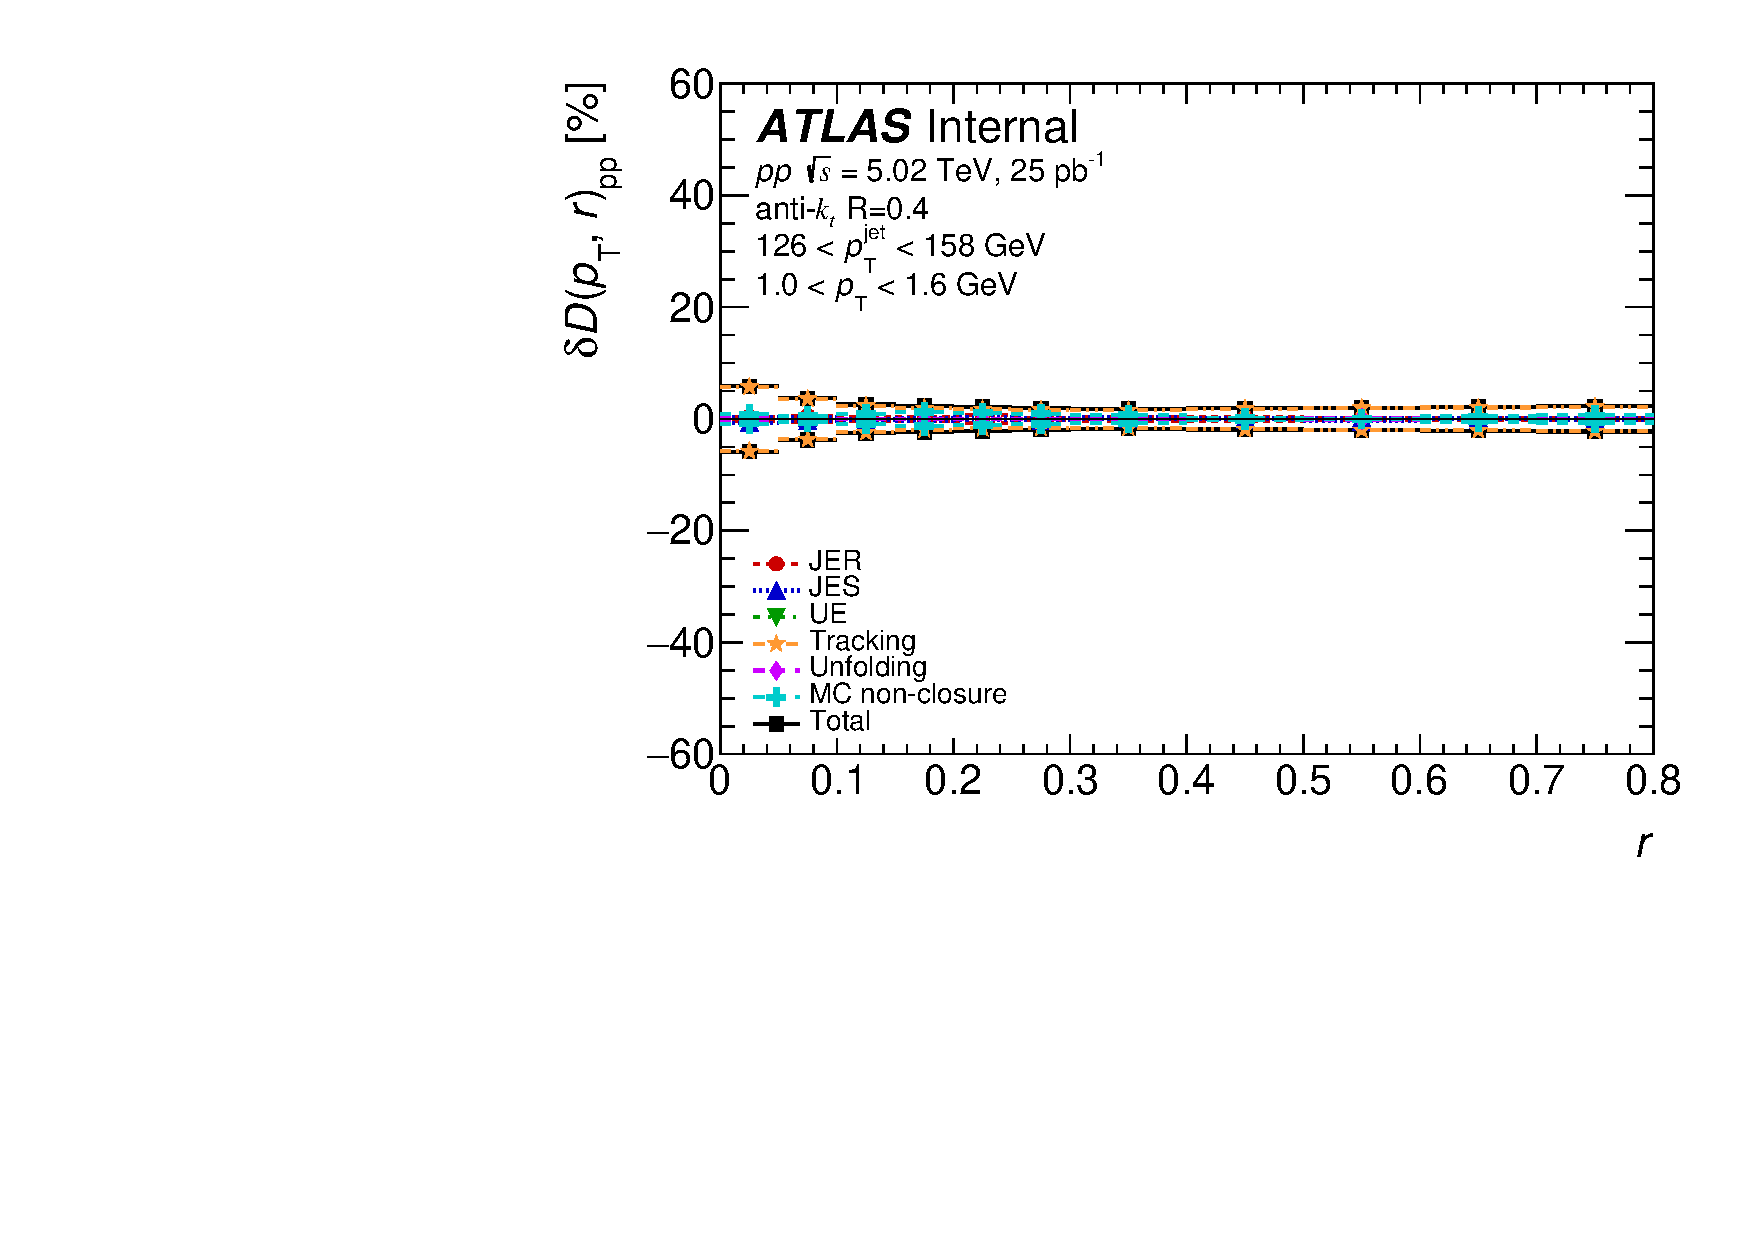
\includegraphics[width=0.53\textwidth]{figures/systematics/ChPS_dR_sys_pp_error_trk2_jet7_cent6} &
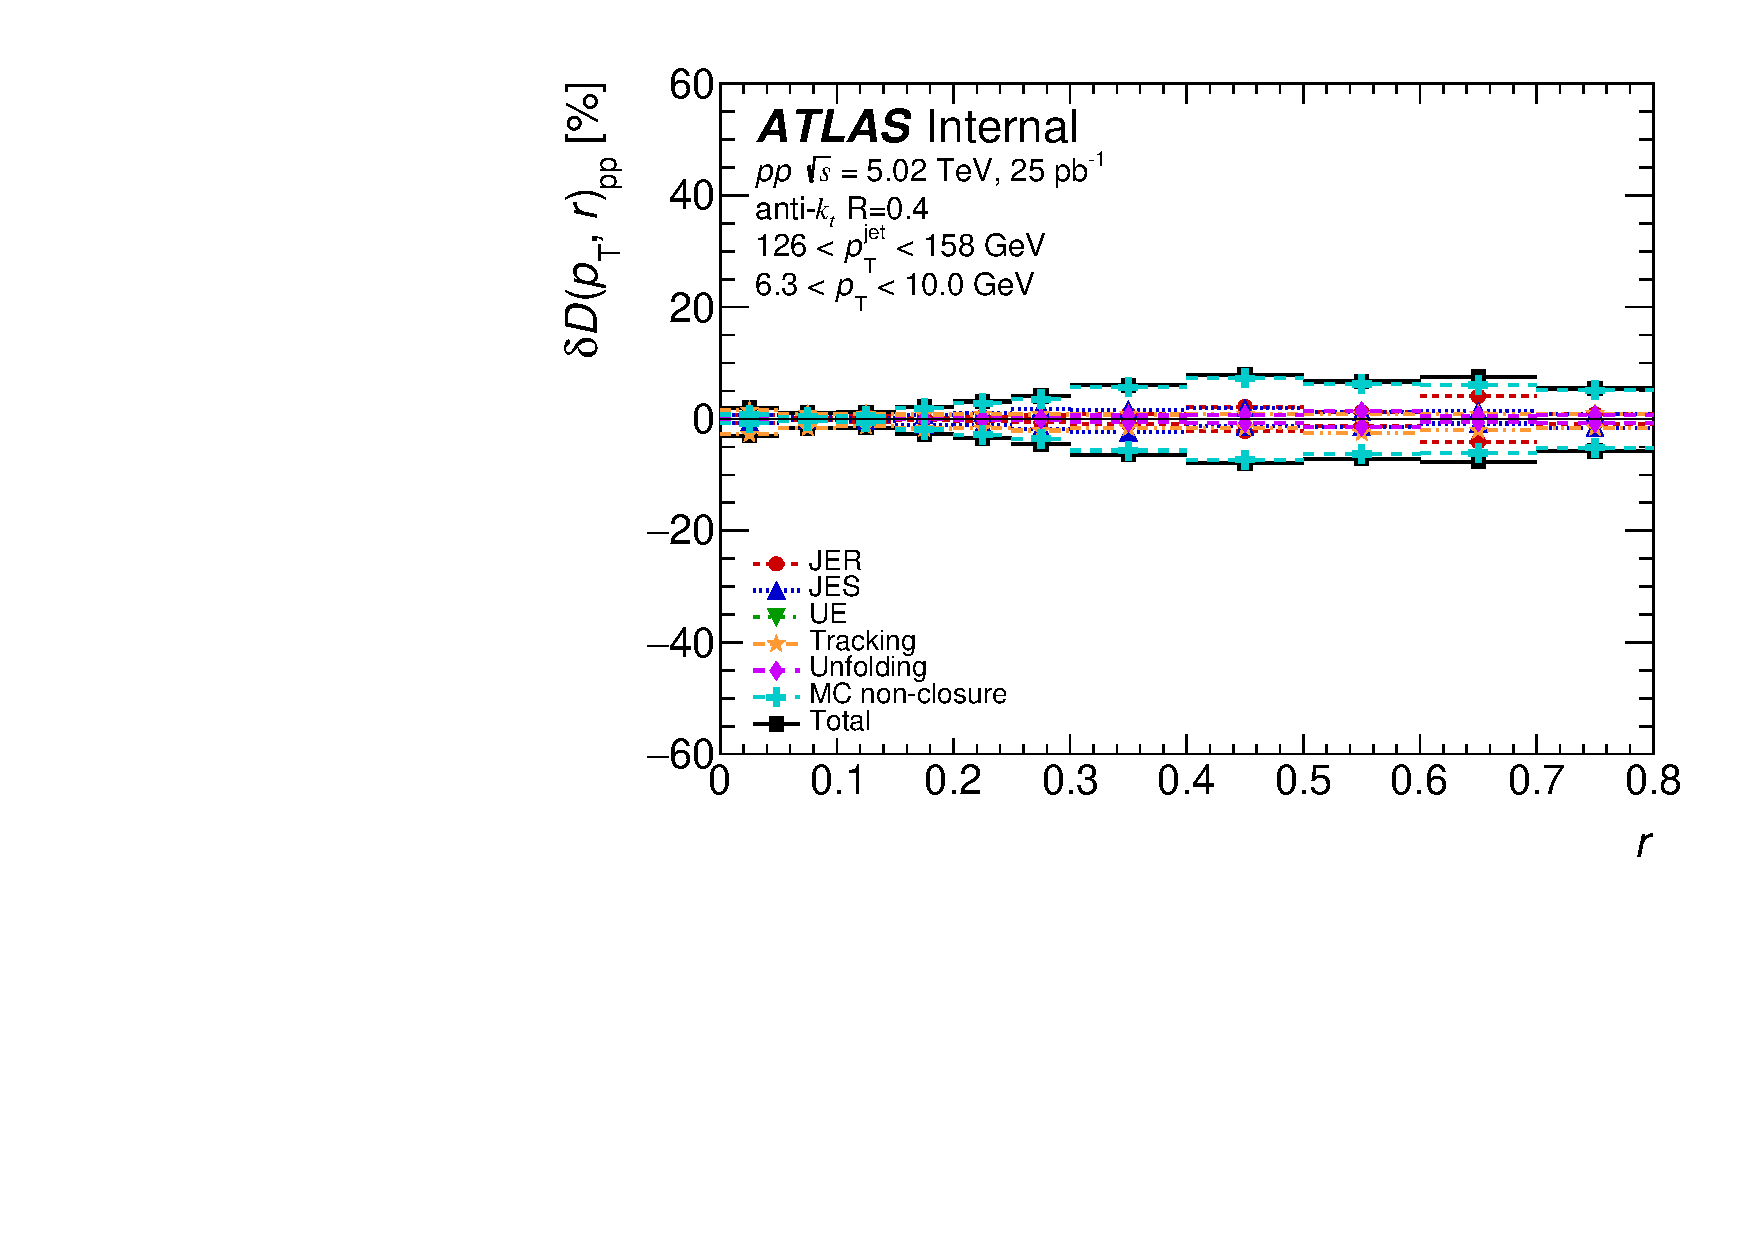
\includegraphics[width=0.53\textwidth]{figures/systematics/ChPS_dR_sys_pp_error_trk6_jet7_cent6} \\
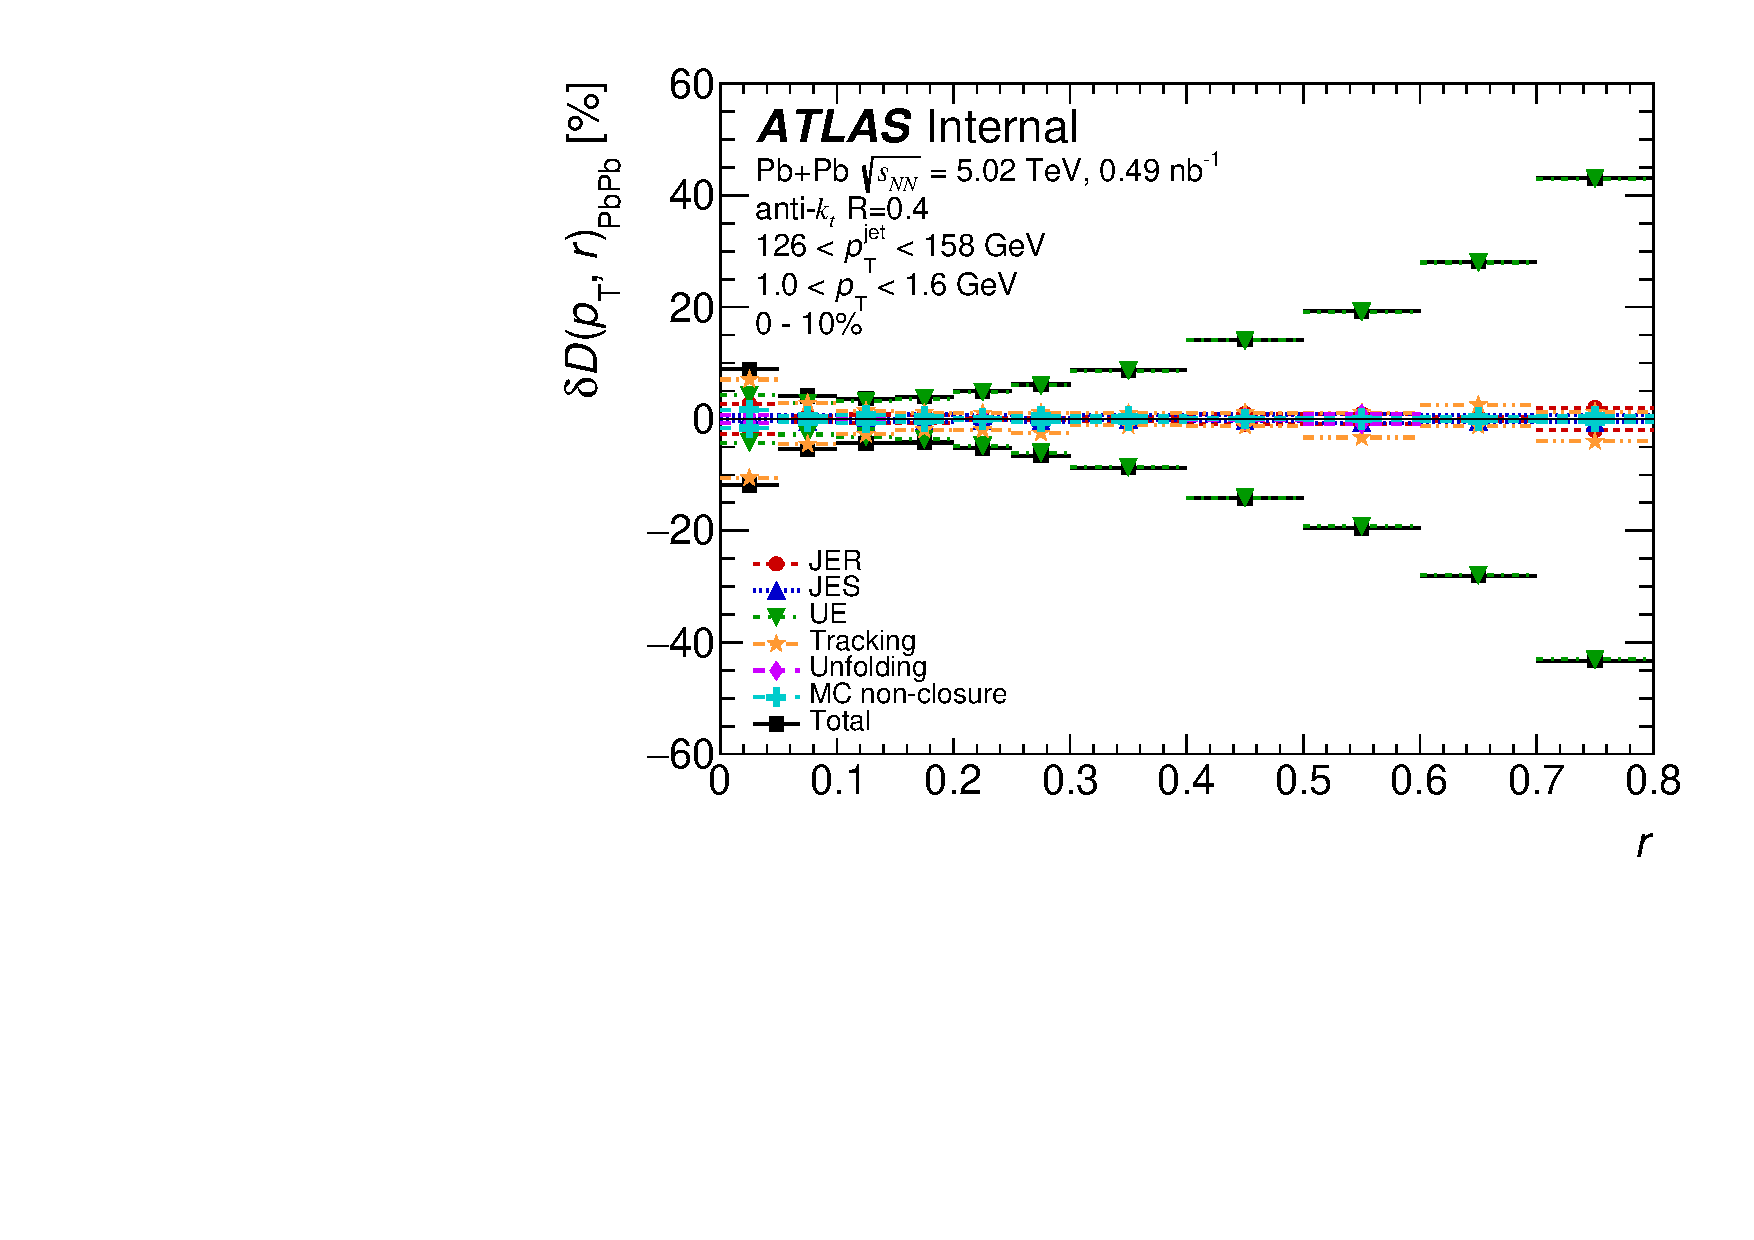
\includegraphics[width=0.53\textwidth]{figures/systematics/ChPS_dR_sys_PbPb_error_trk2_jet7_cent0} &
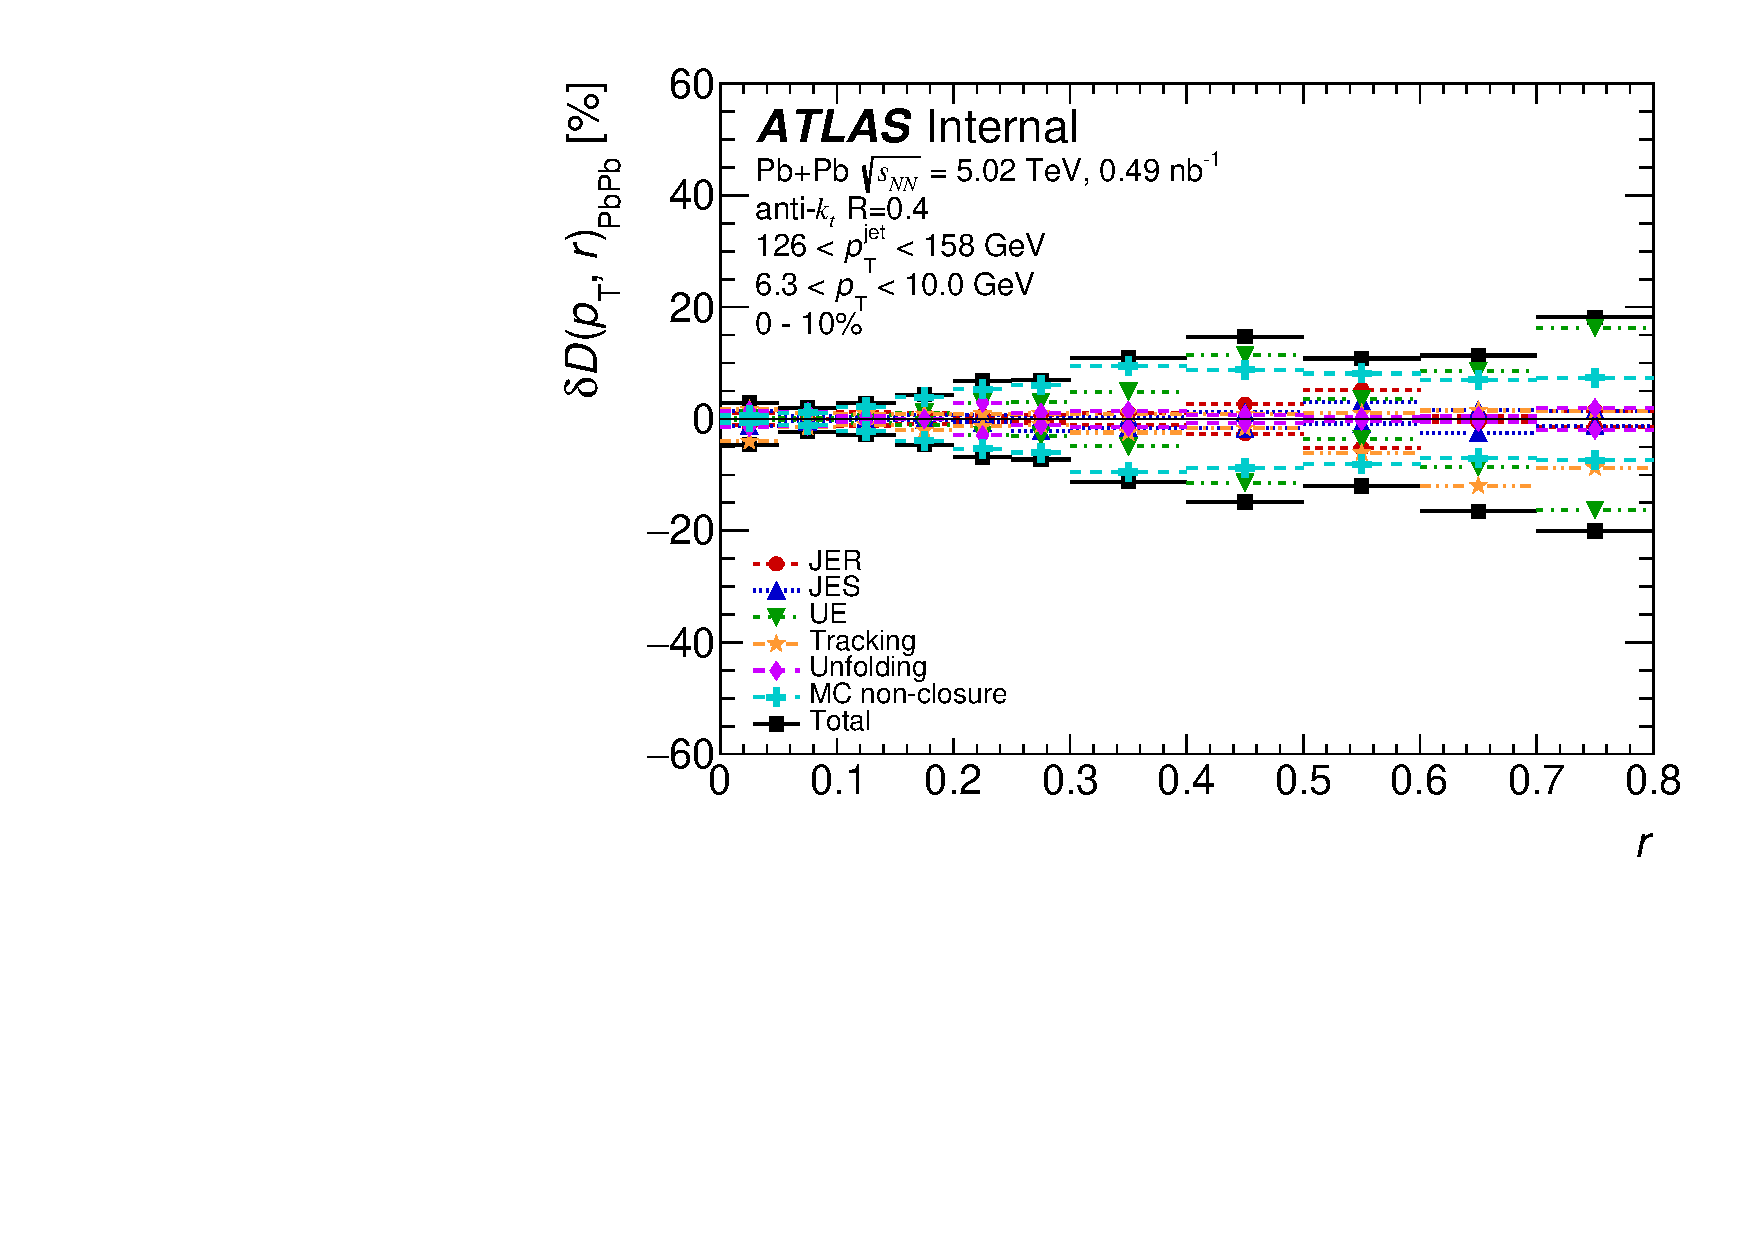
\includegraphics[width=0.53\textwidth]{figures/systematics/ChPS_dR_sys_PbPb_error_trk6_jet7_cent0} \\
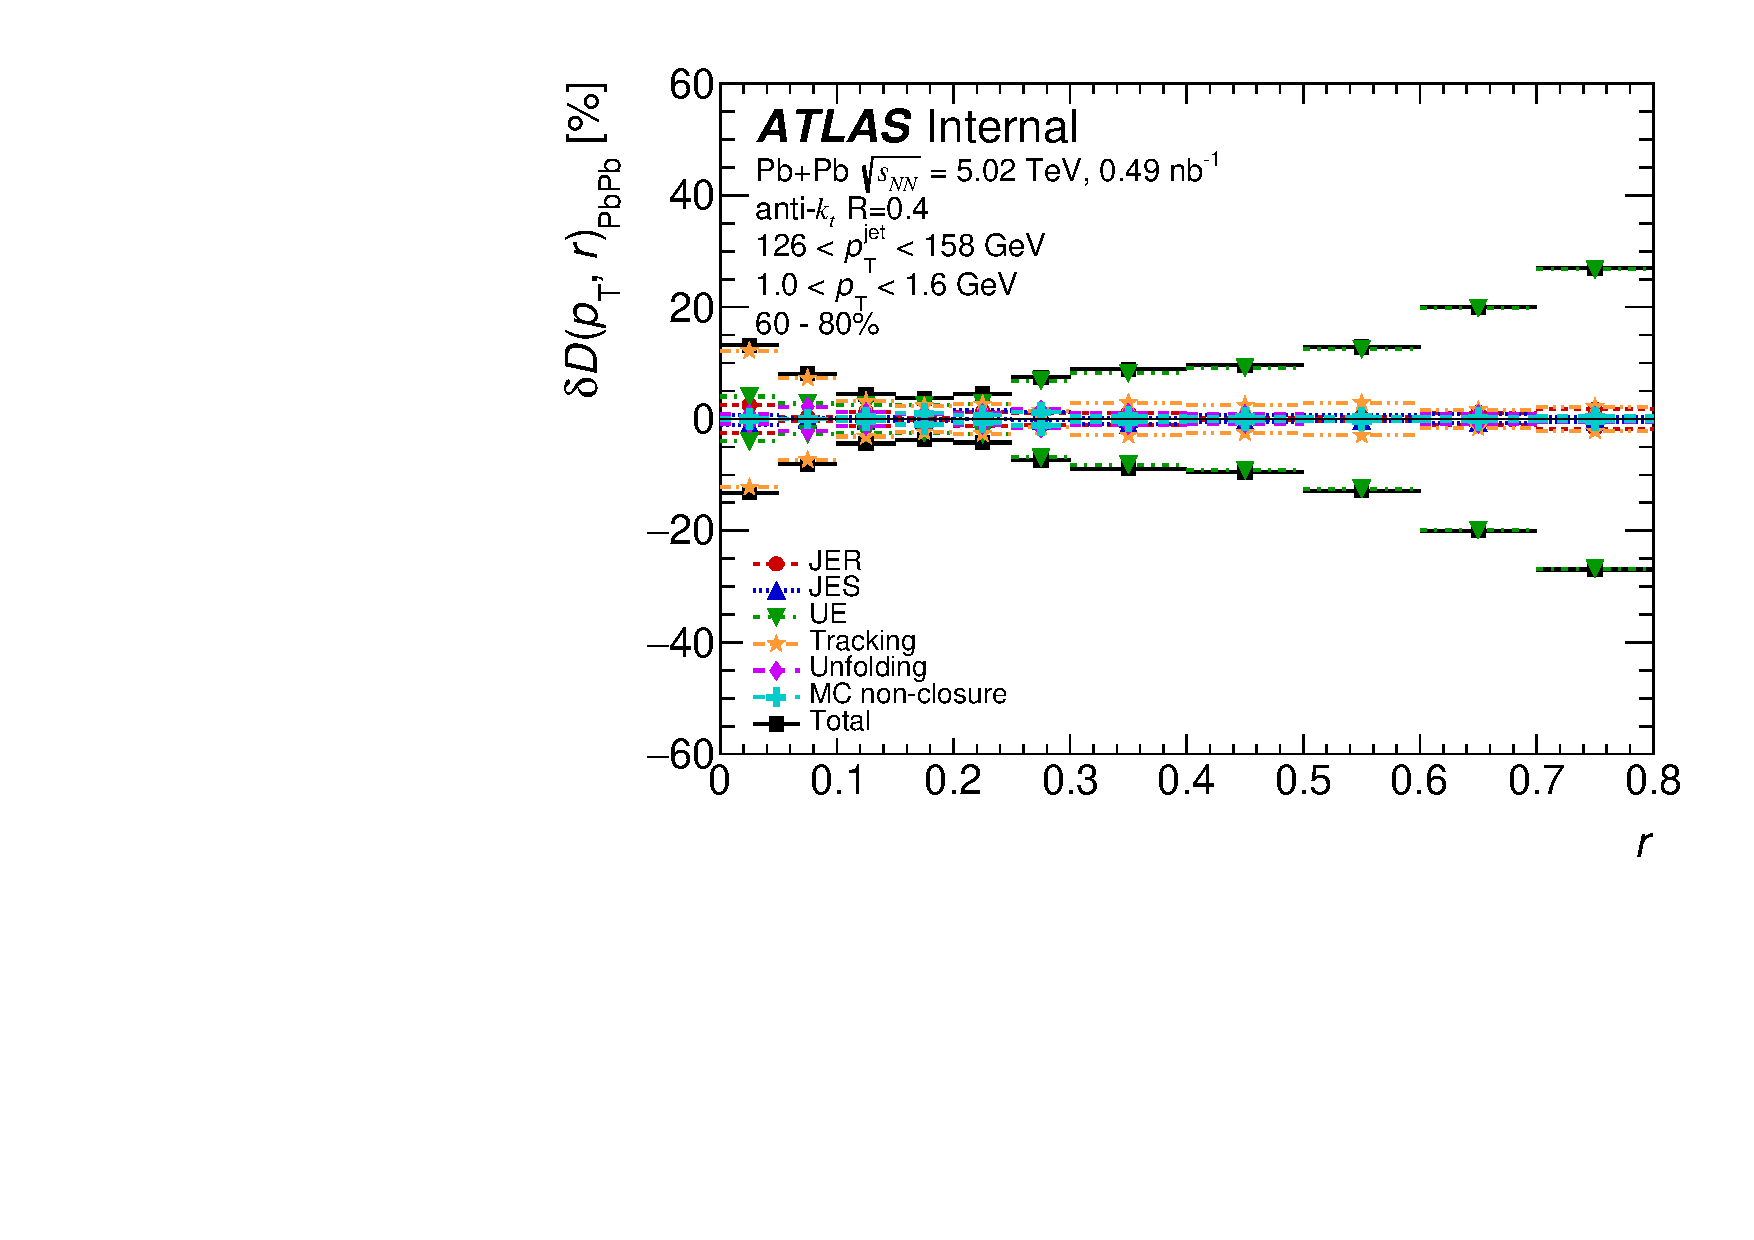
\includegraphics[width=0.53\textwidth]{figures/systematics/ChPS_dR_sys_PbPb_error_trk2_jet7_cent5} &
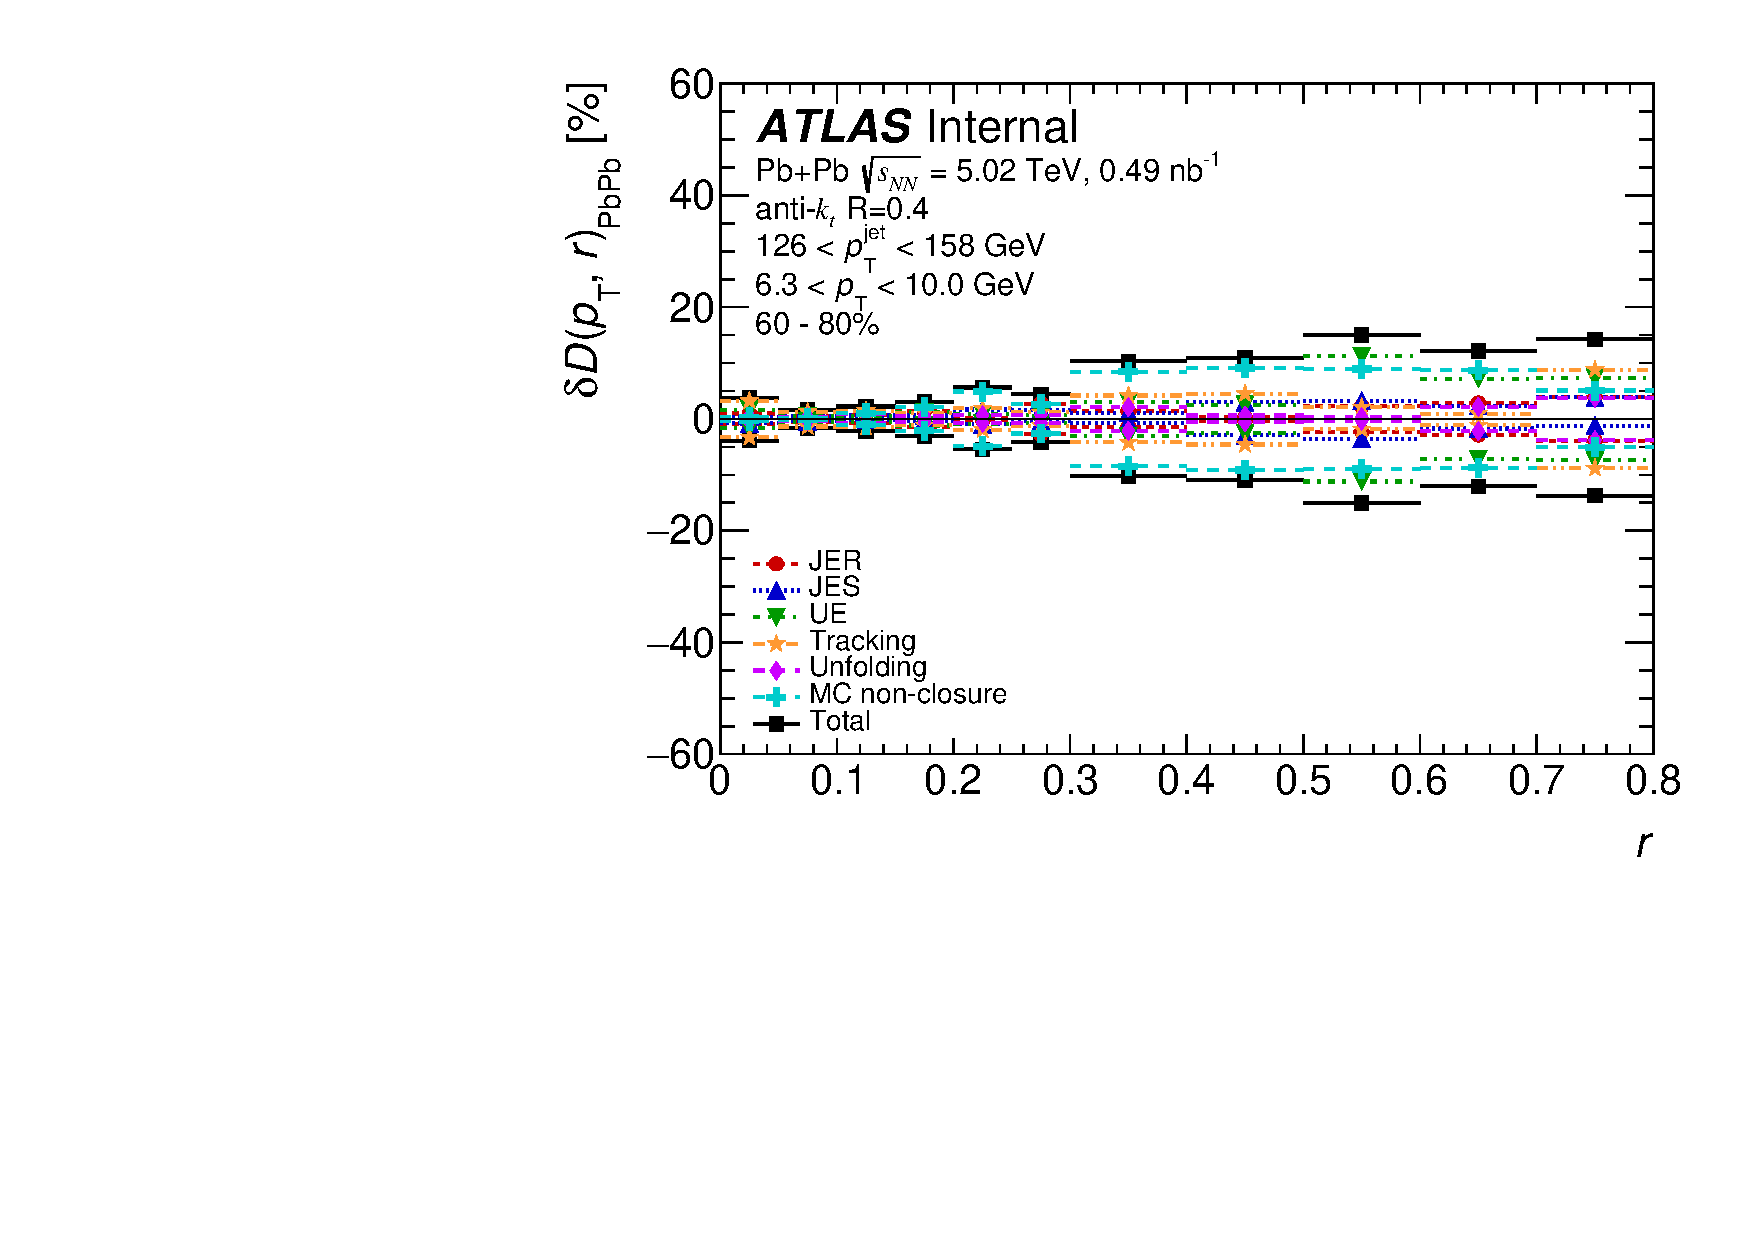
\includegraphics[width=0.53\textwidth]{figures/systematics/ChPS_dR_sys_PbPb_error_trk6_jet7_cent5} \\
\end{tabular}}
\caption{
Relative size of the systematic uncertainties for \Dptr\ distributions in \pp\ (top), central 0--10\% \pbpb\ (middle), and peripheral 60--80\% \pbpb\ (bottom) collisions for tracks with $1.0 < \pt < 1.6$ \GeV\ (left) and $6.3 < \pt < 10$ \GeV\ (right) in jets with $126 < \ptjet < 158$ \GeV. The systematic uncertainties due to JES, JER, unfolding, UE contribution, MC non-closure, and tracking are shown along with the total systematic uncertainty from all sources.
}
\label{fig:Systematics_Dpt}
\end{figure}

\begin{figure}
\centerline{
\begin{tabular}{cc}
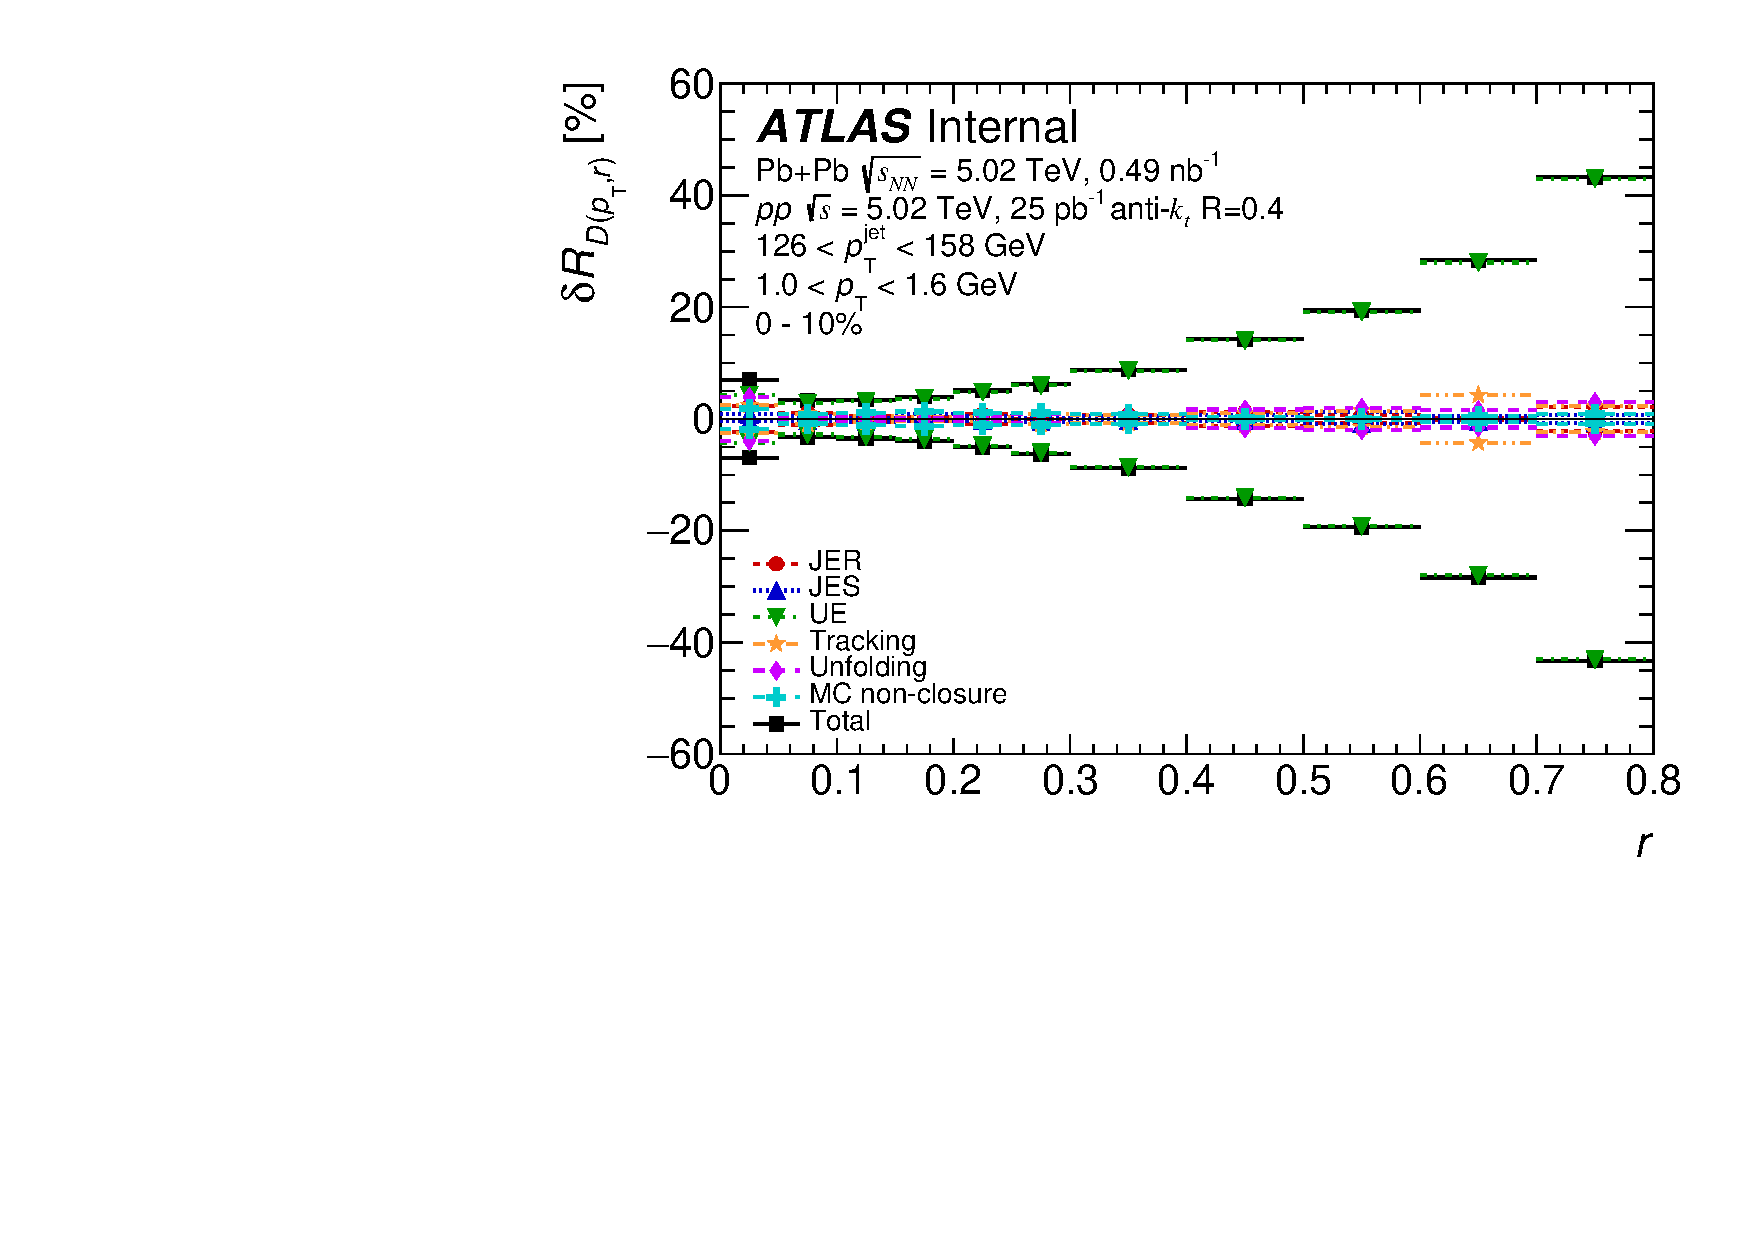
\includegraphics[width=0.53\textwidth]{figures/systematics/RDpT_dR_sys_error_trk2_jet7_cent0} &
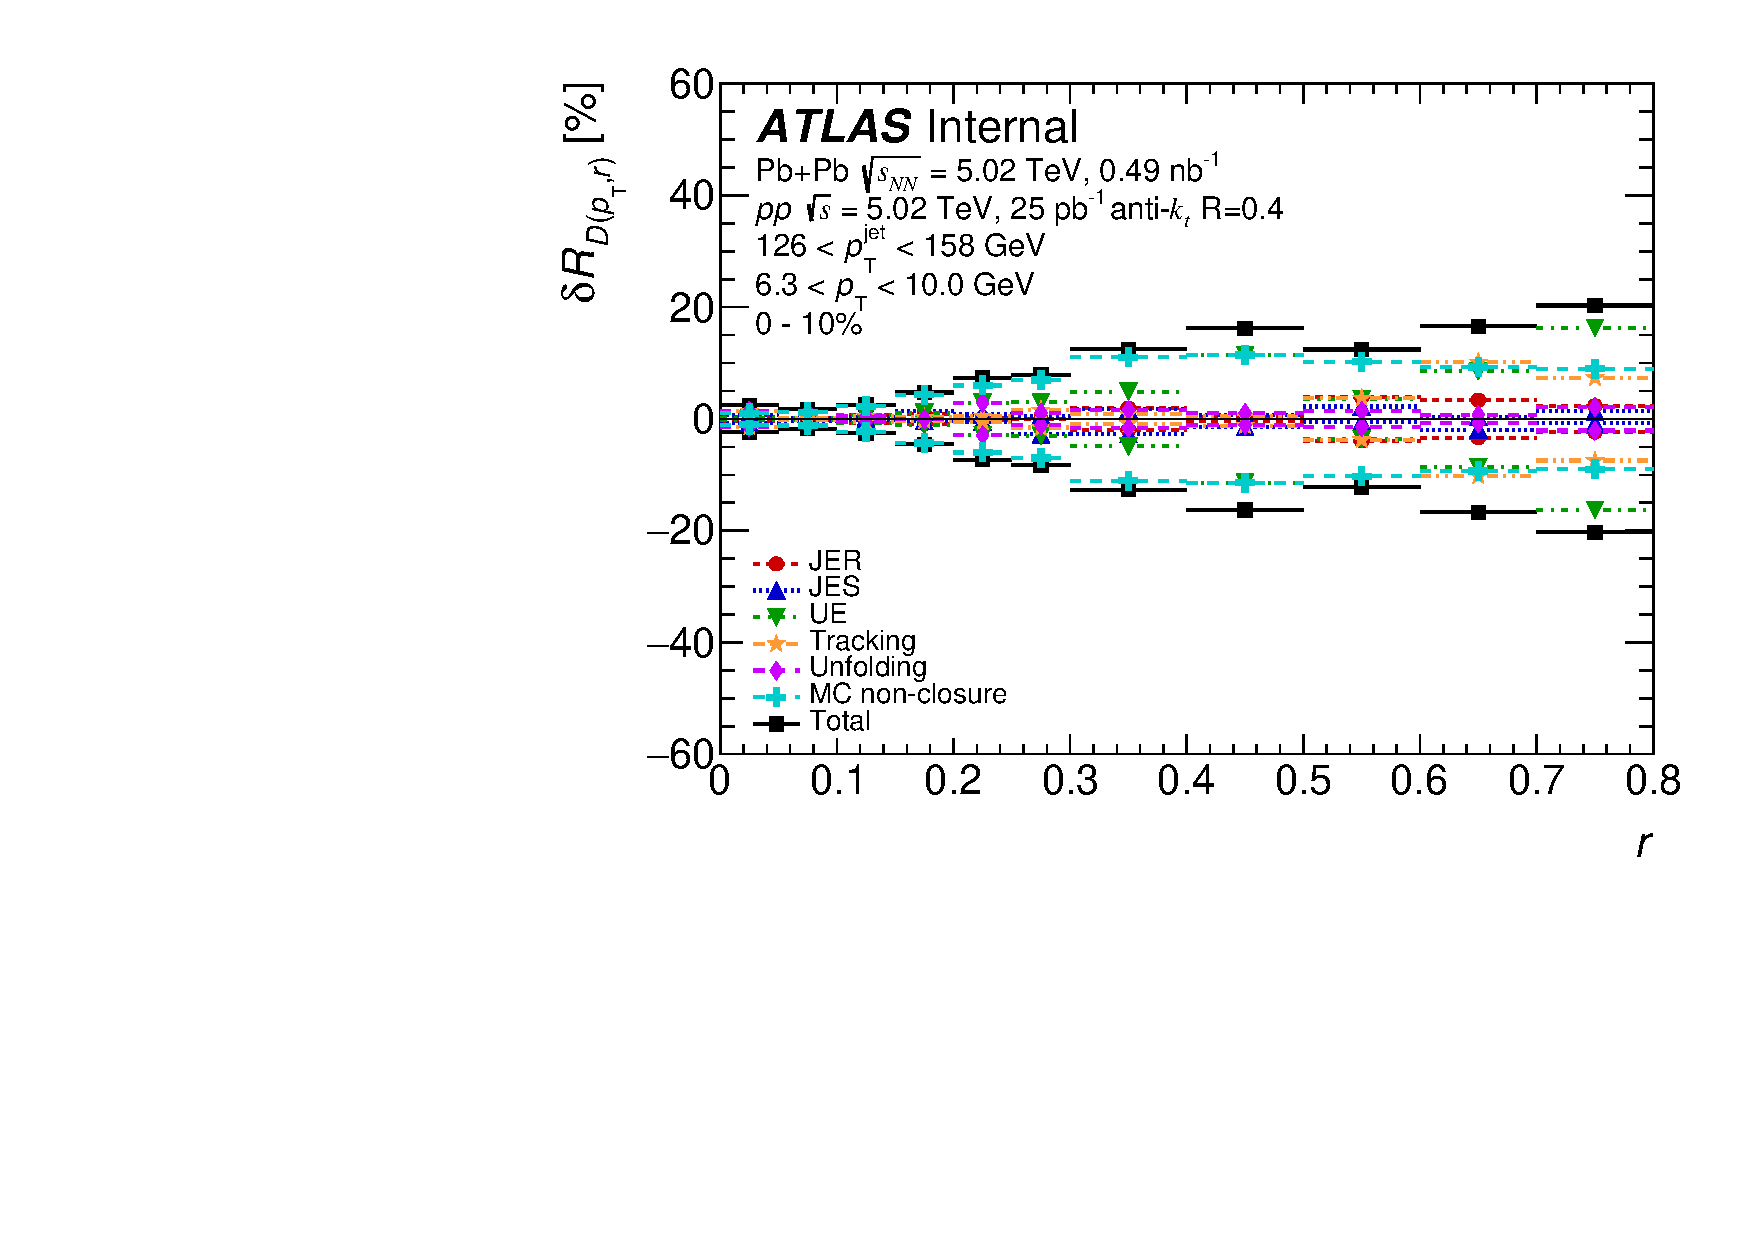
\includegraphics[width=0.53\textwidth]{figures/systematics/RDpT_dR_sys_error_trk6_jet7_cent0} \\
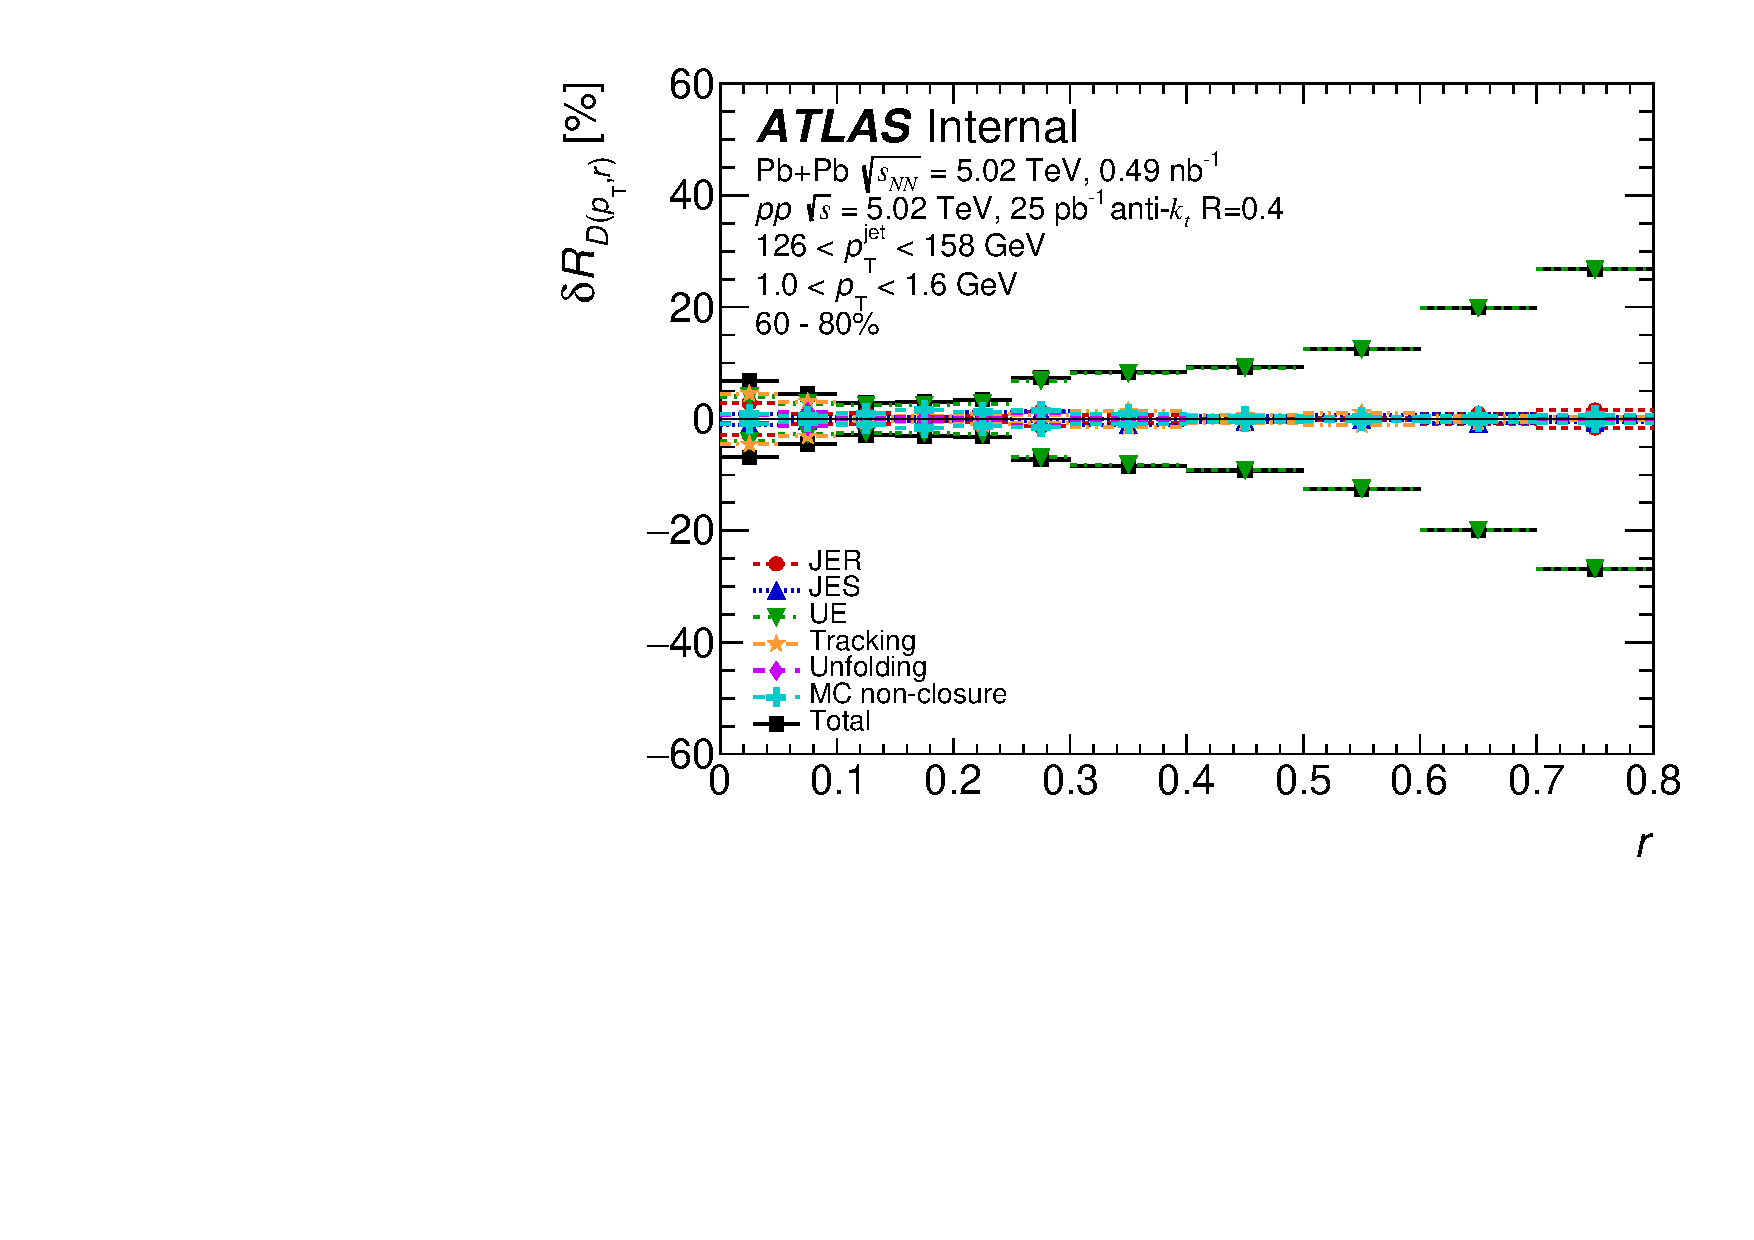
\includegraphics[width=0.53\textwidth]{figures/systematics/RDpT_dR_sys_error_trk2_jet7_cent5} &
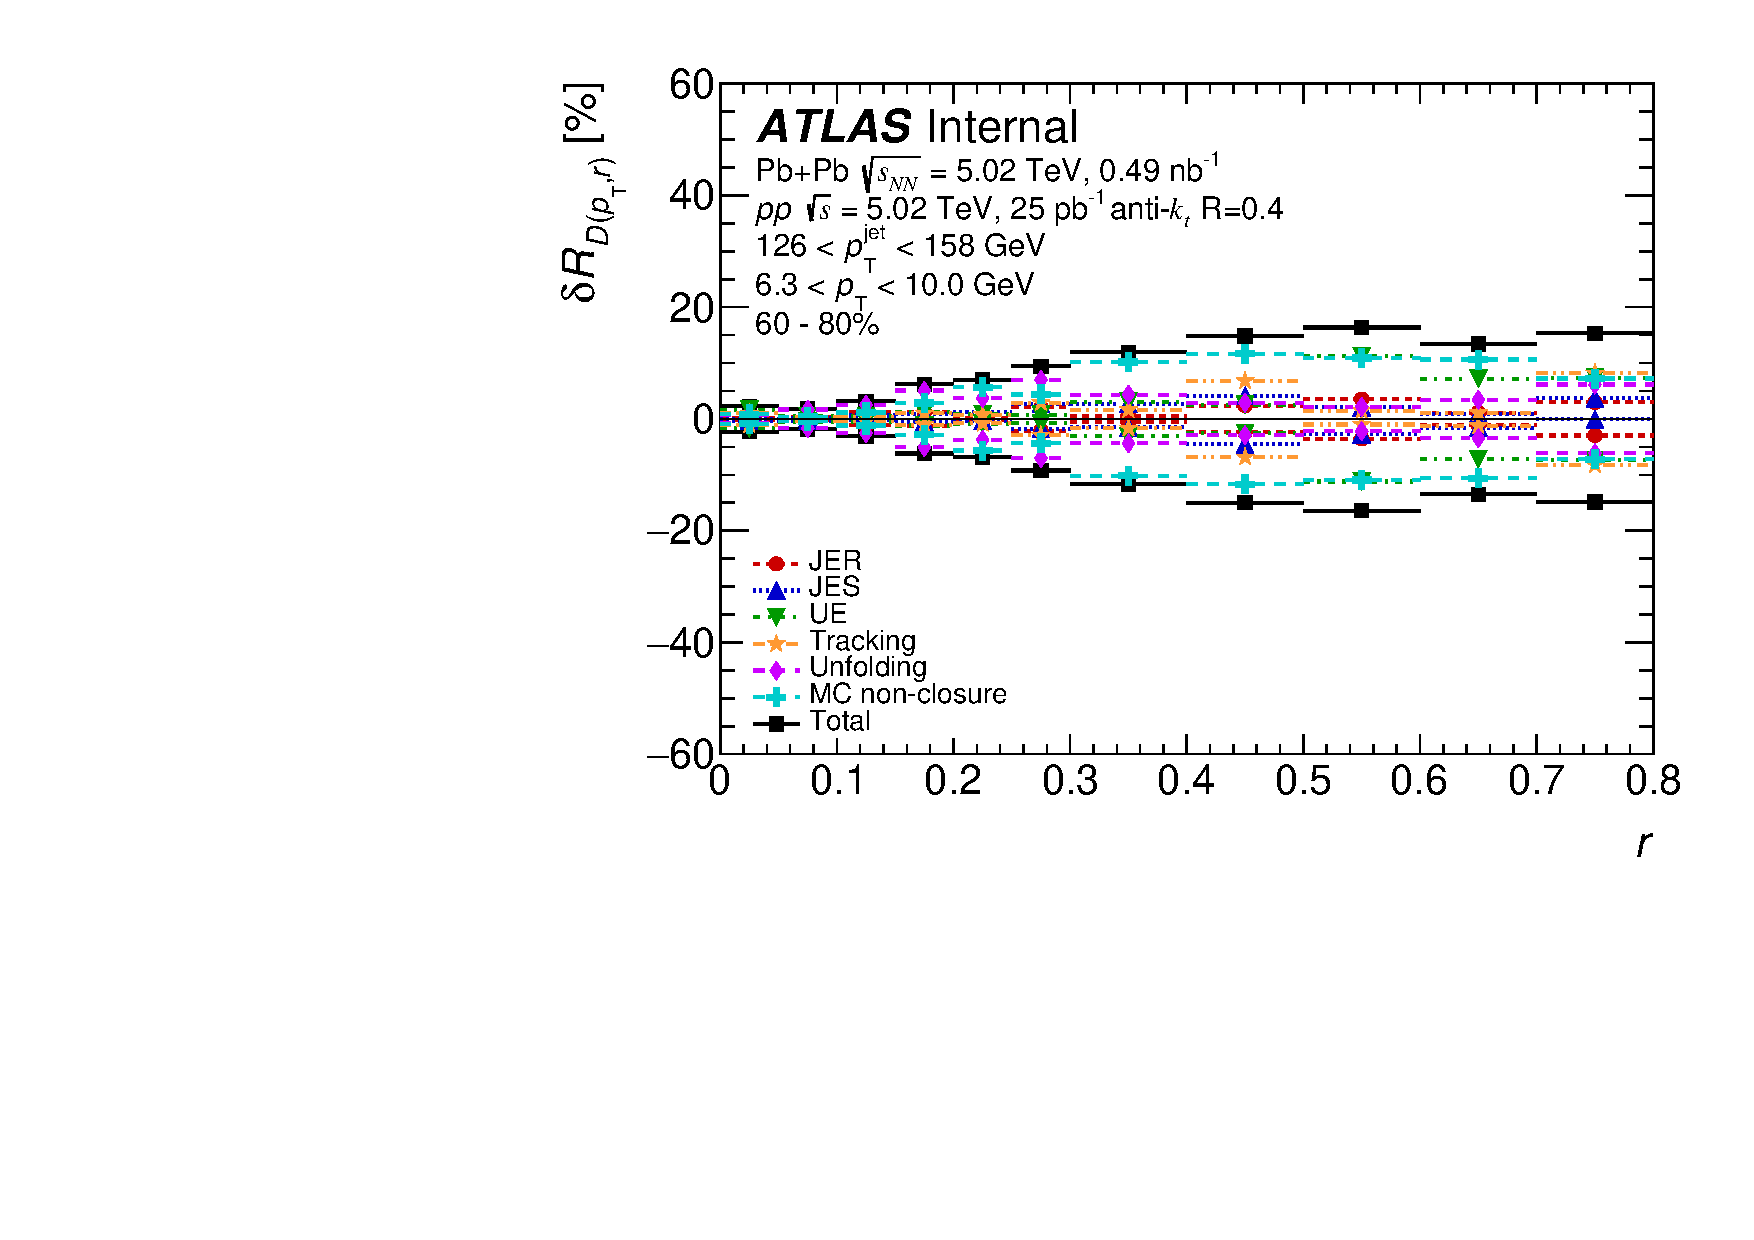
\includegraphics[width=0.53\textwidth]{figures/systematics/RDpT_dR_sys_error_trk6_jet7_cent5} \\
\end{tabular}}
\caption{
Relative size of the systematic uncertainties for \RDptr\ distributions for 0--10\% (top) and 60--80\% (bottom) \pbpb\ collisions, for tracks with $1.0 < \pt < 1.6$ \GeV\ (left) and $6.3 < \pt < 10.0$ \GeV\ (right), in jets with $126 < \ptjet < 158$ \GeV. The systematic uncertainties due to JES, JER, unfolding, UE contribution, MC non-closure, and tracking are shown along with the total systematic uncertainty from all sources.
}
\label{fig:Systematics_RDpT}
\end{figure}

%\begin{figure}
%\centerline{
%\begin{tabular}{cc}
%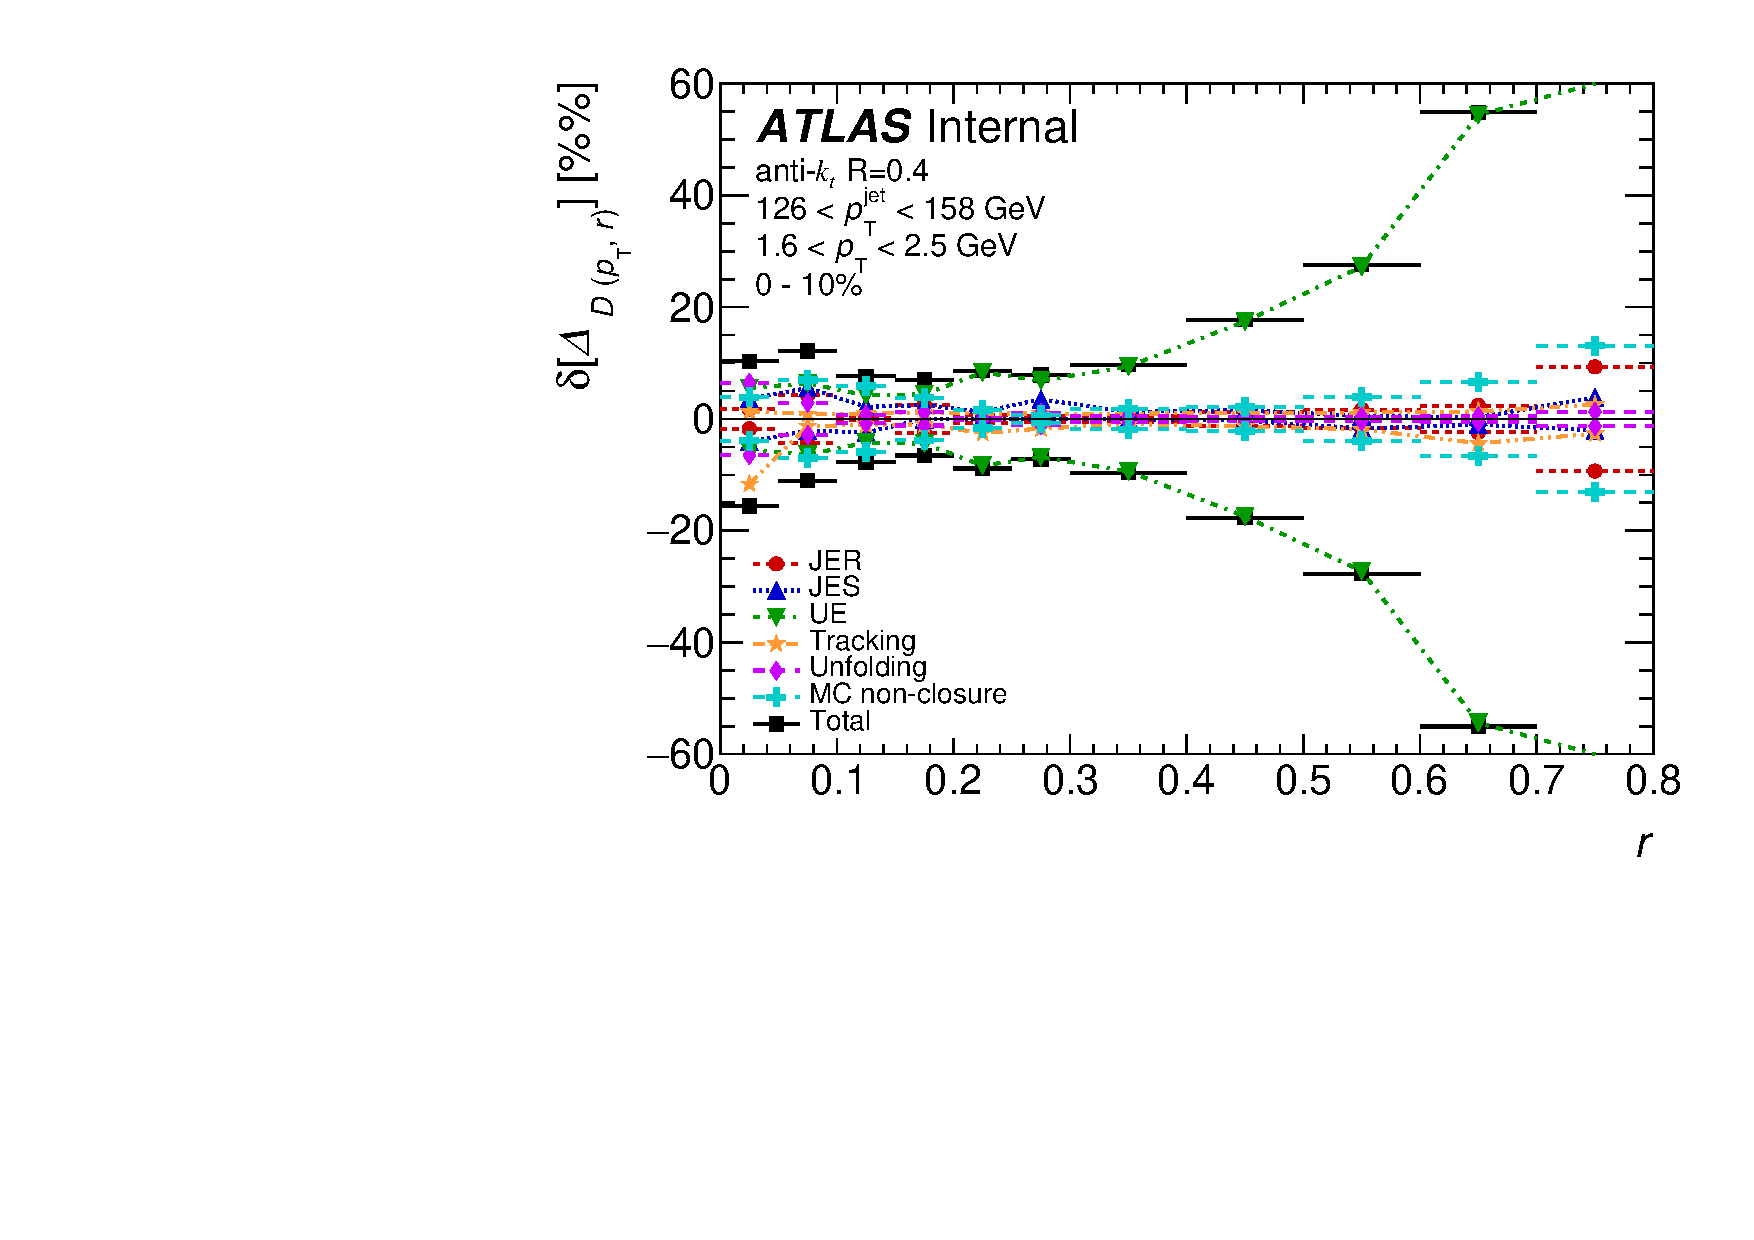
\includegraphics[width=0.55\textwidth]{figures/systematics/DeltaDpT_dR_sys_error_trk3_jet7_cent0} &
%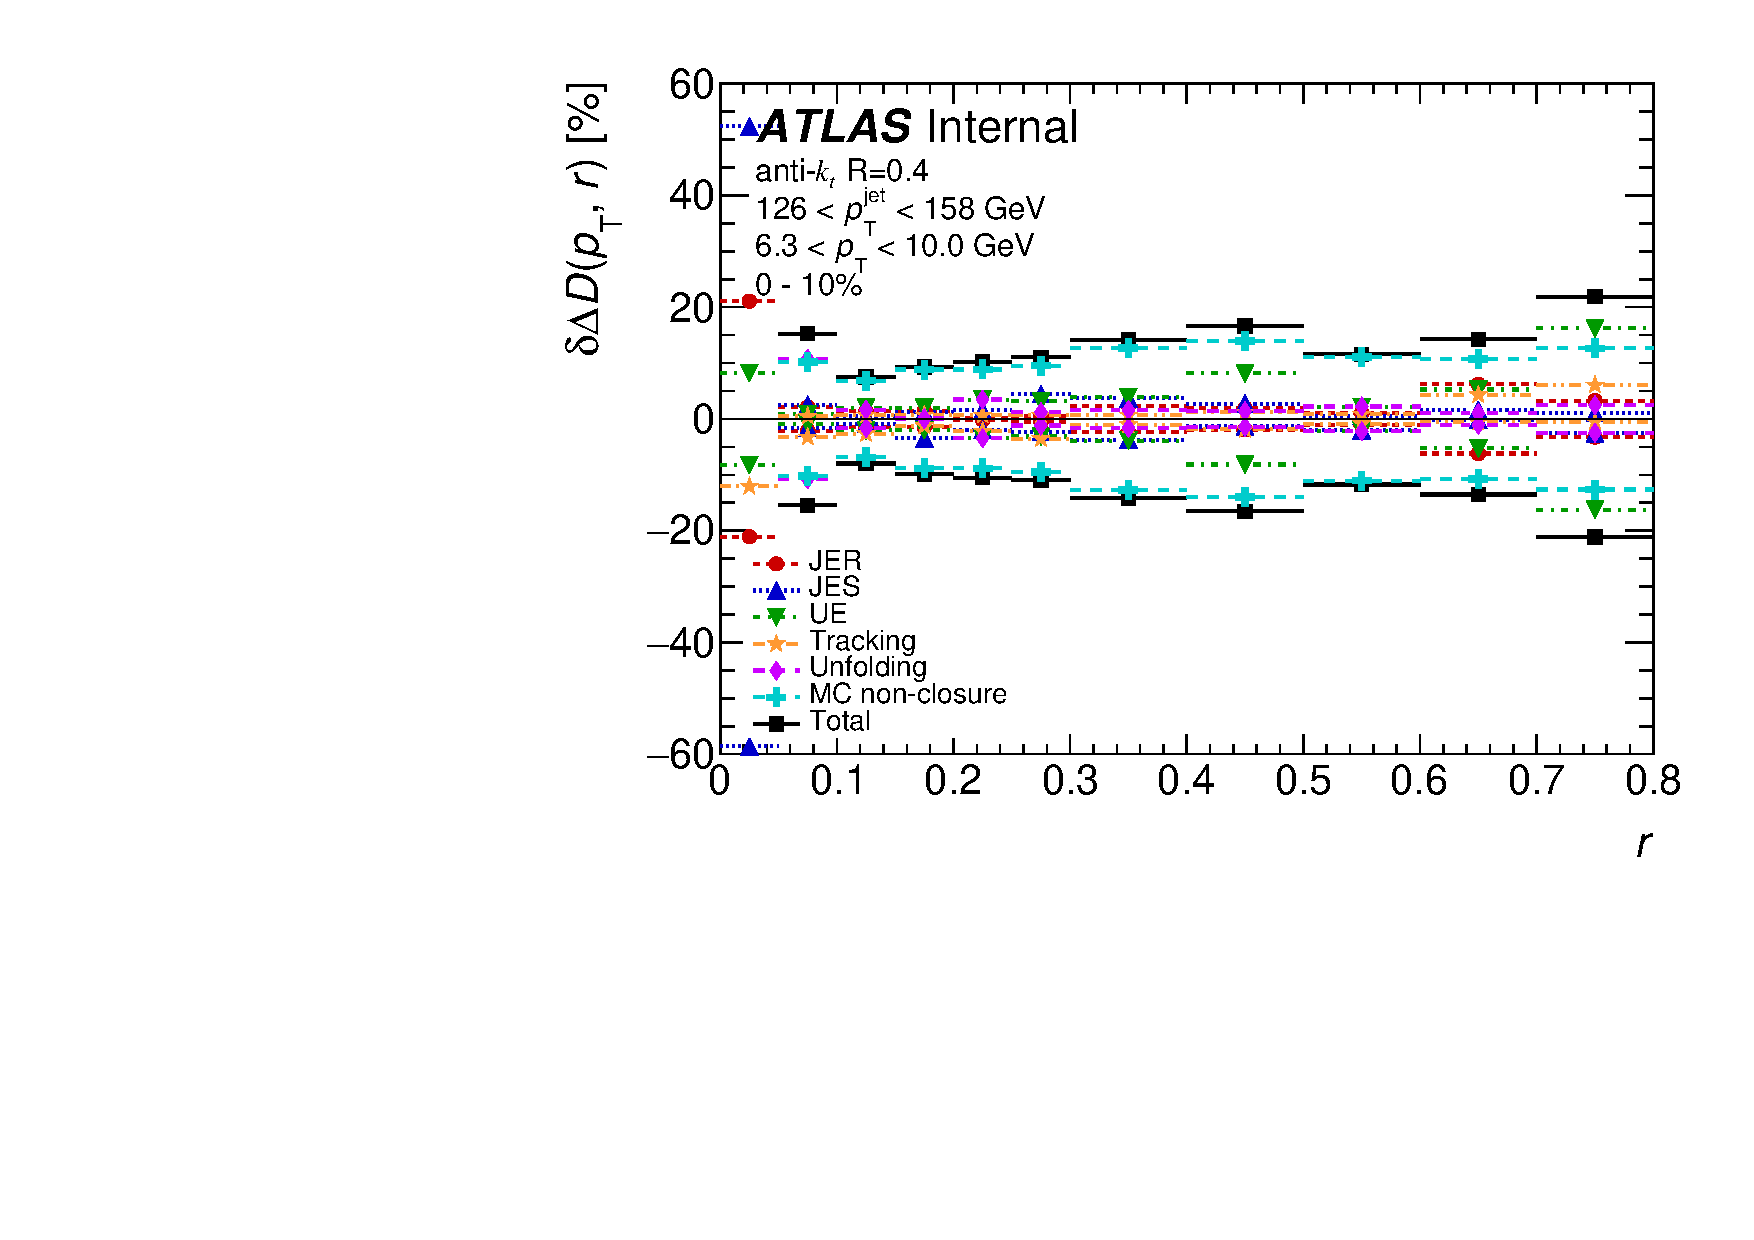
\includegraphics[width=0.55\textwidth]{figures/systematics/DeltaDpT_dR_sys_error_trk6_jet7_cent0} \\
%\end{tabular}}
%\caption{
%Relative size of the systematic uncertainties for $\Delta\Dptr$ distributions for 0--10\% \pbpb\ collisions, for tracks in the \pt\ range 1.0--1.6 \GeV\ (left) and 6.3--10.0 \GeV\ (right), in jets with $126 < \ptjet < 158$ \GeV. The systematic uncertainties due to JES, JER, unfolding, UE contribution, MC non-closure and tracking are shown along with the total systematic uncertainty from all sources.
%}
%\label{fig:Systematics_DeltaDpT}
%\end{figure}


%-------------------------------------------------------------------------------
\section{Results}
\label{sec:results}
% !TEX root = trkjet.tex

The \Dptr\ distributions are studied as a function of \ptjet\ for \pp\ data and \PbPb\ collisions with different centralities. Ratios and differences between \Dptr\ distributions in \pbpb\ and \pp\ collisions are evaluated to explore the interplay between the hot and dense matter and the parton shower.

The \Dptr\ distributions evaluated in \pp\ and \pbpb\ collisions for $126 < \ptjet < 158$ GeV are shown in Figure~\ref{fig:dptr}. The distributions exhibit a difference in shape between \PbPb\ and the \pp\ reference, with the \pbpb\ distributions being broader at low \pt\ (\pt < 4 GeV) and narrower at high \pt\ (\pt > 4 GeV) in \mbox{0--10\%} central collisions. This modification is centrality dependent and is smaller for peripheral \pbpb\ collisions.

\begin{figure}[h]
\centerline{
            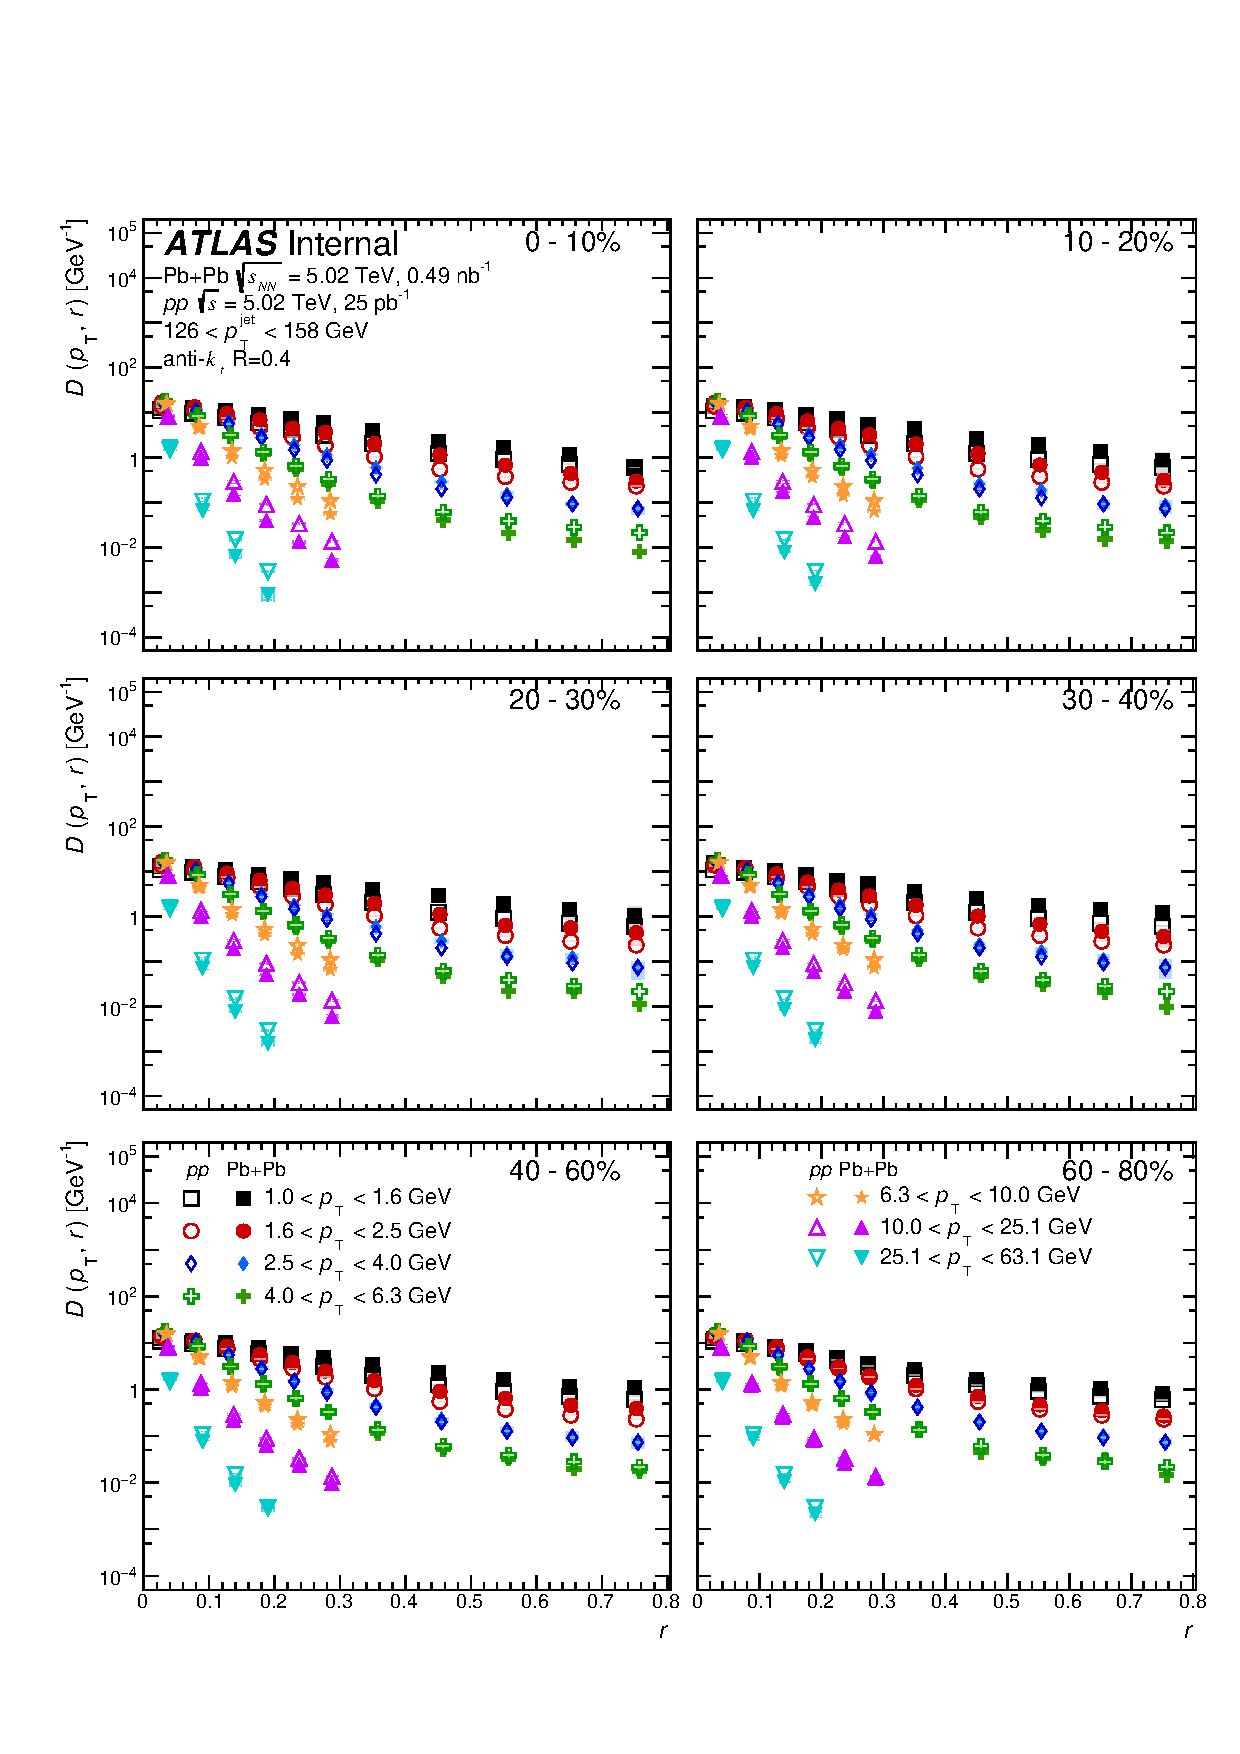
\includegraphics[width=1\textwidth]{figures/results/DpT_dR_jet7.pdf} 
      }
\caption{The \Dptr\ distributions in \pp\ (open symbols) and \pbpb\ (closed symbols) as a function of angular distance $r$ for \ptjet\ of 126 to 158~\GeV. The colors represent different track \pt\ ranges, and each panel is a different centrality selection. The vertical bars on the data points indicate statistical uncertainties while the shaded boxes indicate systematic uncertainties. The widths of the boxes are not indicative of the bin size and the points are shifted horizontally for better visibility.}
\label{fig:dptr}
\end{figure}


Ratios of the \Dptr\ distributions in \pbpb\ to those measured in \pp\ for $126 < \ptjet < 158$ GeV and $200 < \ptjet < 251$ GeV jets and are presented in Figure~\ref{fig:rdptr}. They are shown as a function of $r$ for different \pt\ and centrality selections. In 0--10\% central collisions,
\RDptr\ is above unity for $\rvar < 0.7$ for charged-particles with \pT less than 4~\GeV\ in both jet selections. 
For these particles, 
the enhancement of the charged particle spectra grows with increasing \rvar\ up to \mbox{$\rvar  = 0.3$}. It is approximately constant over \mbox{0.3 -- 0.6} and decreases for \mbox{$\rvar > 0.6$}.  For charged particles with $\pt > 4.0$ \GeV, \RDptr\ shows a depletion outside the jet core for $r > 0.05$. The magnitude of this depletion increases with increasing \rvar\ up to $r = 0.3$ and is approximately constant thereafter.
 The observed behavior inside the jet ($r < 0.4$) agrees with the measurement of the inclusive jet fragmentation functions~\cite{Aaboud:2017eww, PhysRevC.98.024908}, where yields of fragments with $\pt < 4$ GeV are observed to be enhanced and yields of charged particles with intermediate \pT\ are suppressed in \PbPb\ collisions compared to those in \pp\ for collisions. 
For peripheral collisions, \RDptr\ has no significant \rvar\ dependence and the distributions do not significantly deviate from unity. 

\begin{figure}[h]
\centerline{
         \begin{tabular}{cc}
            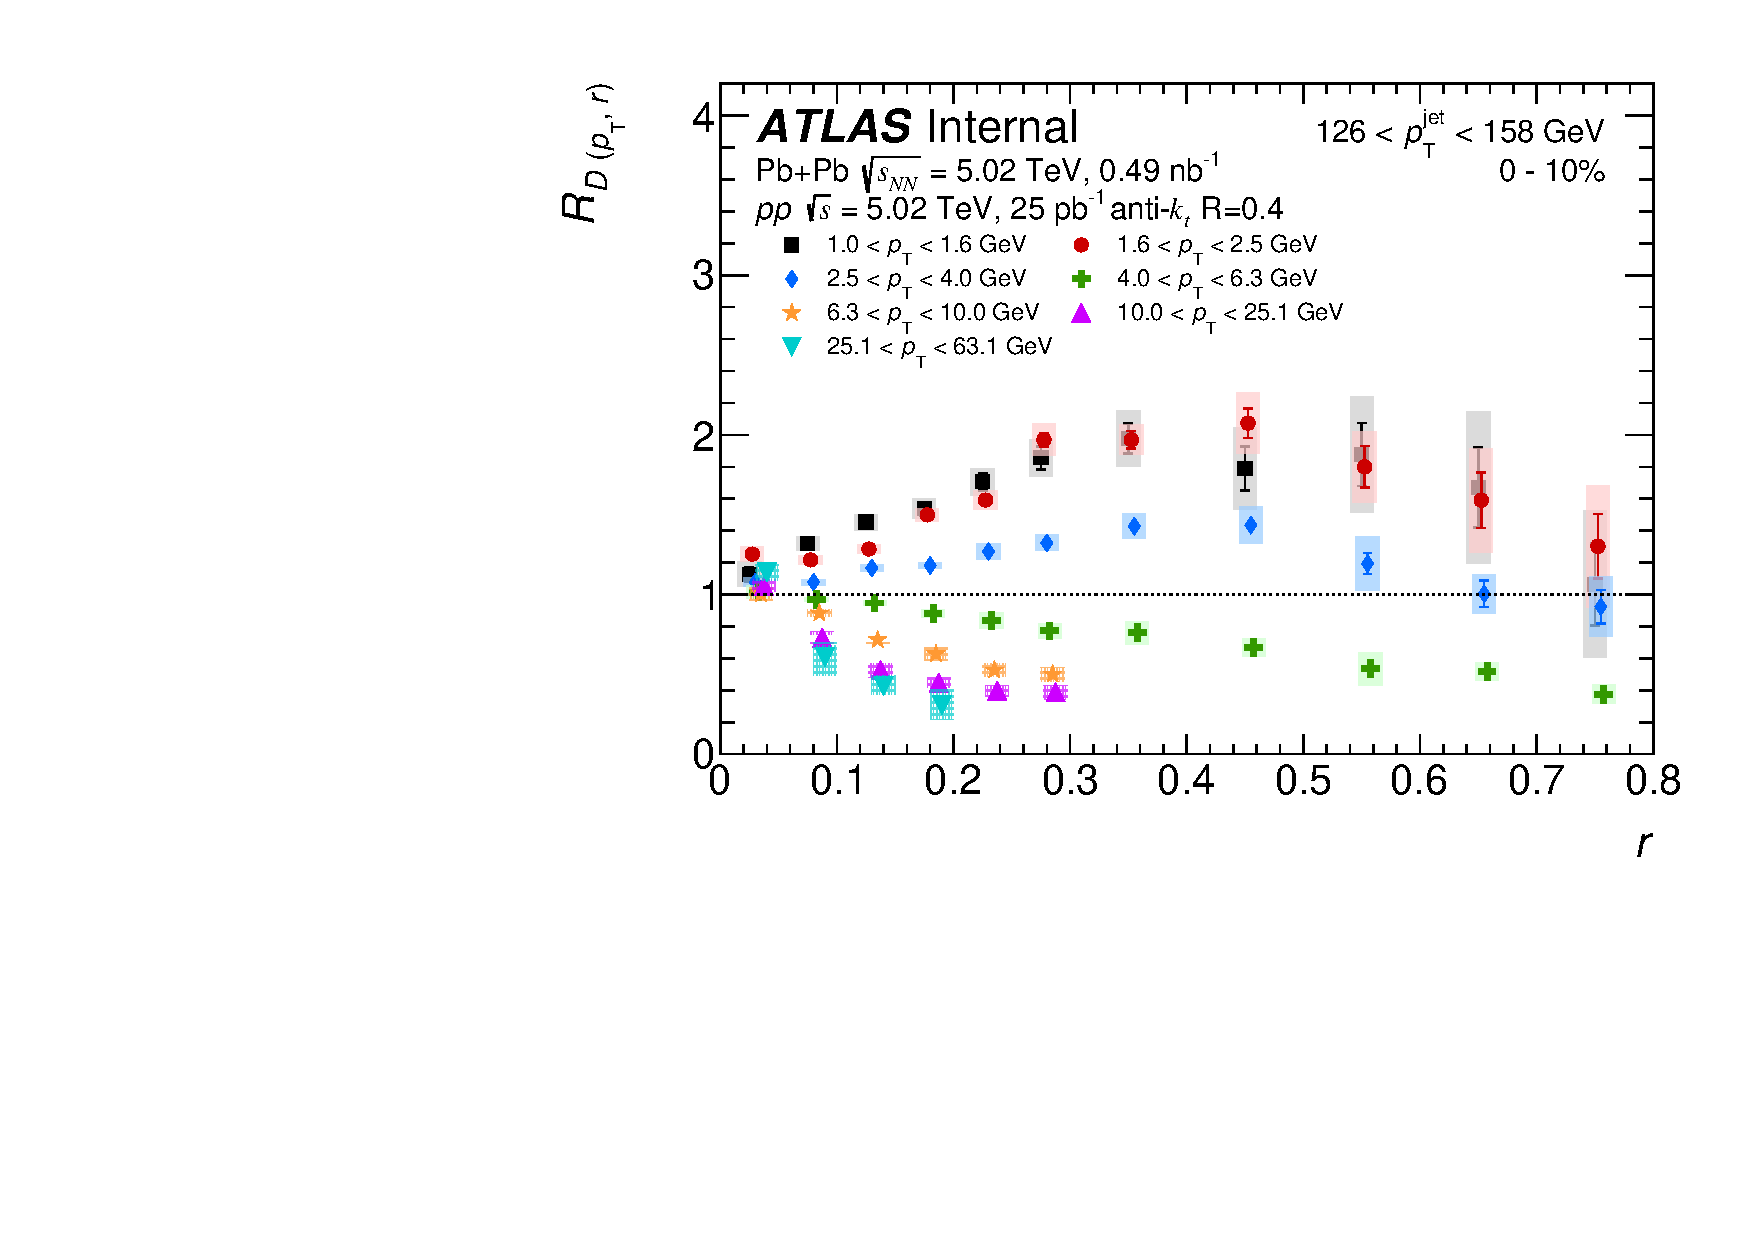
\includegraphics[width=0.5\textwidth]{figures/results/RDpT_dR_jet7_cent0.pdf} & 
            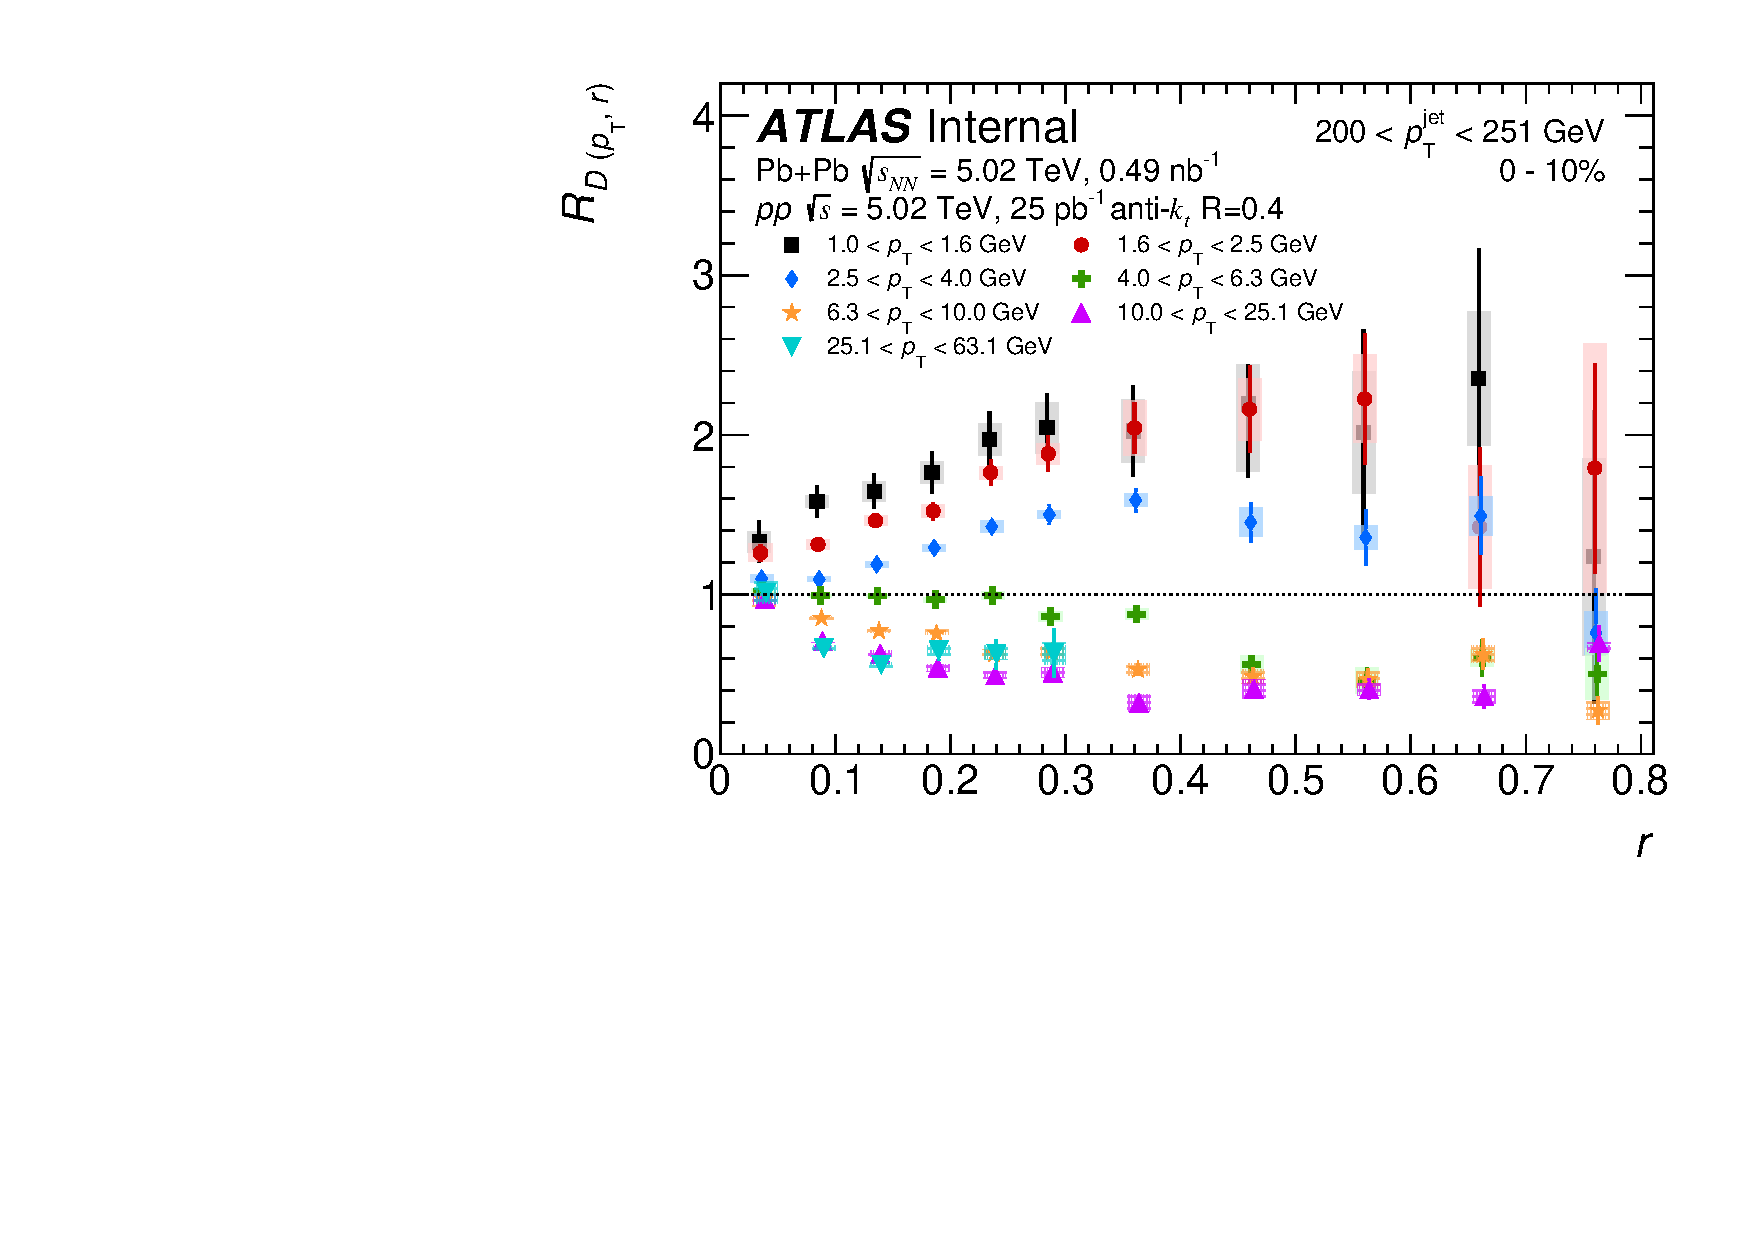
\includegraphics[width=0.5\textwidth]{figures/results/RDpT_dR_jet9_cent0.pdf} \\
            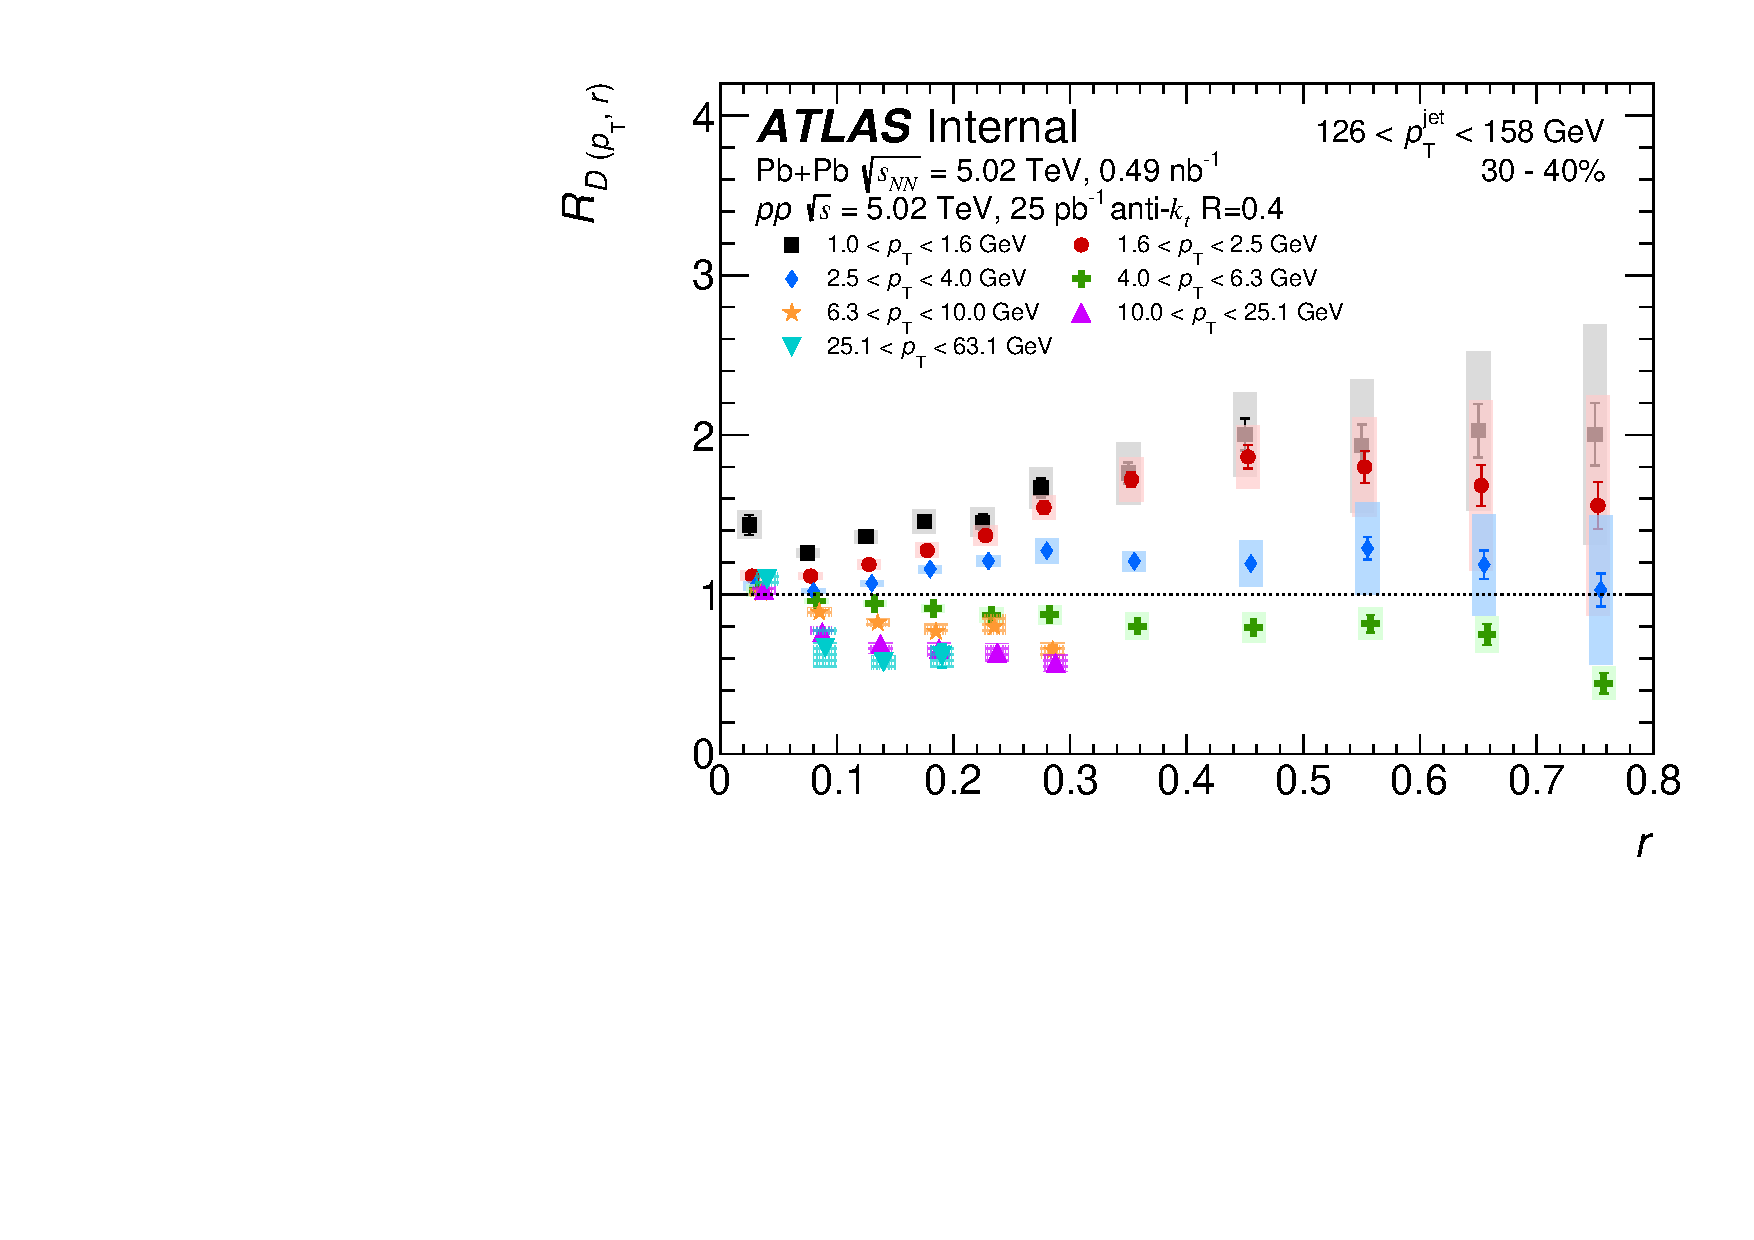
\includegraphics[width=0.5\textwidth]{figures/results/RDpT_dR_jet7_cent3.pdf} & 
            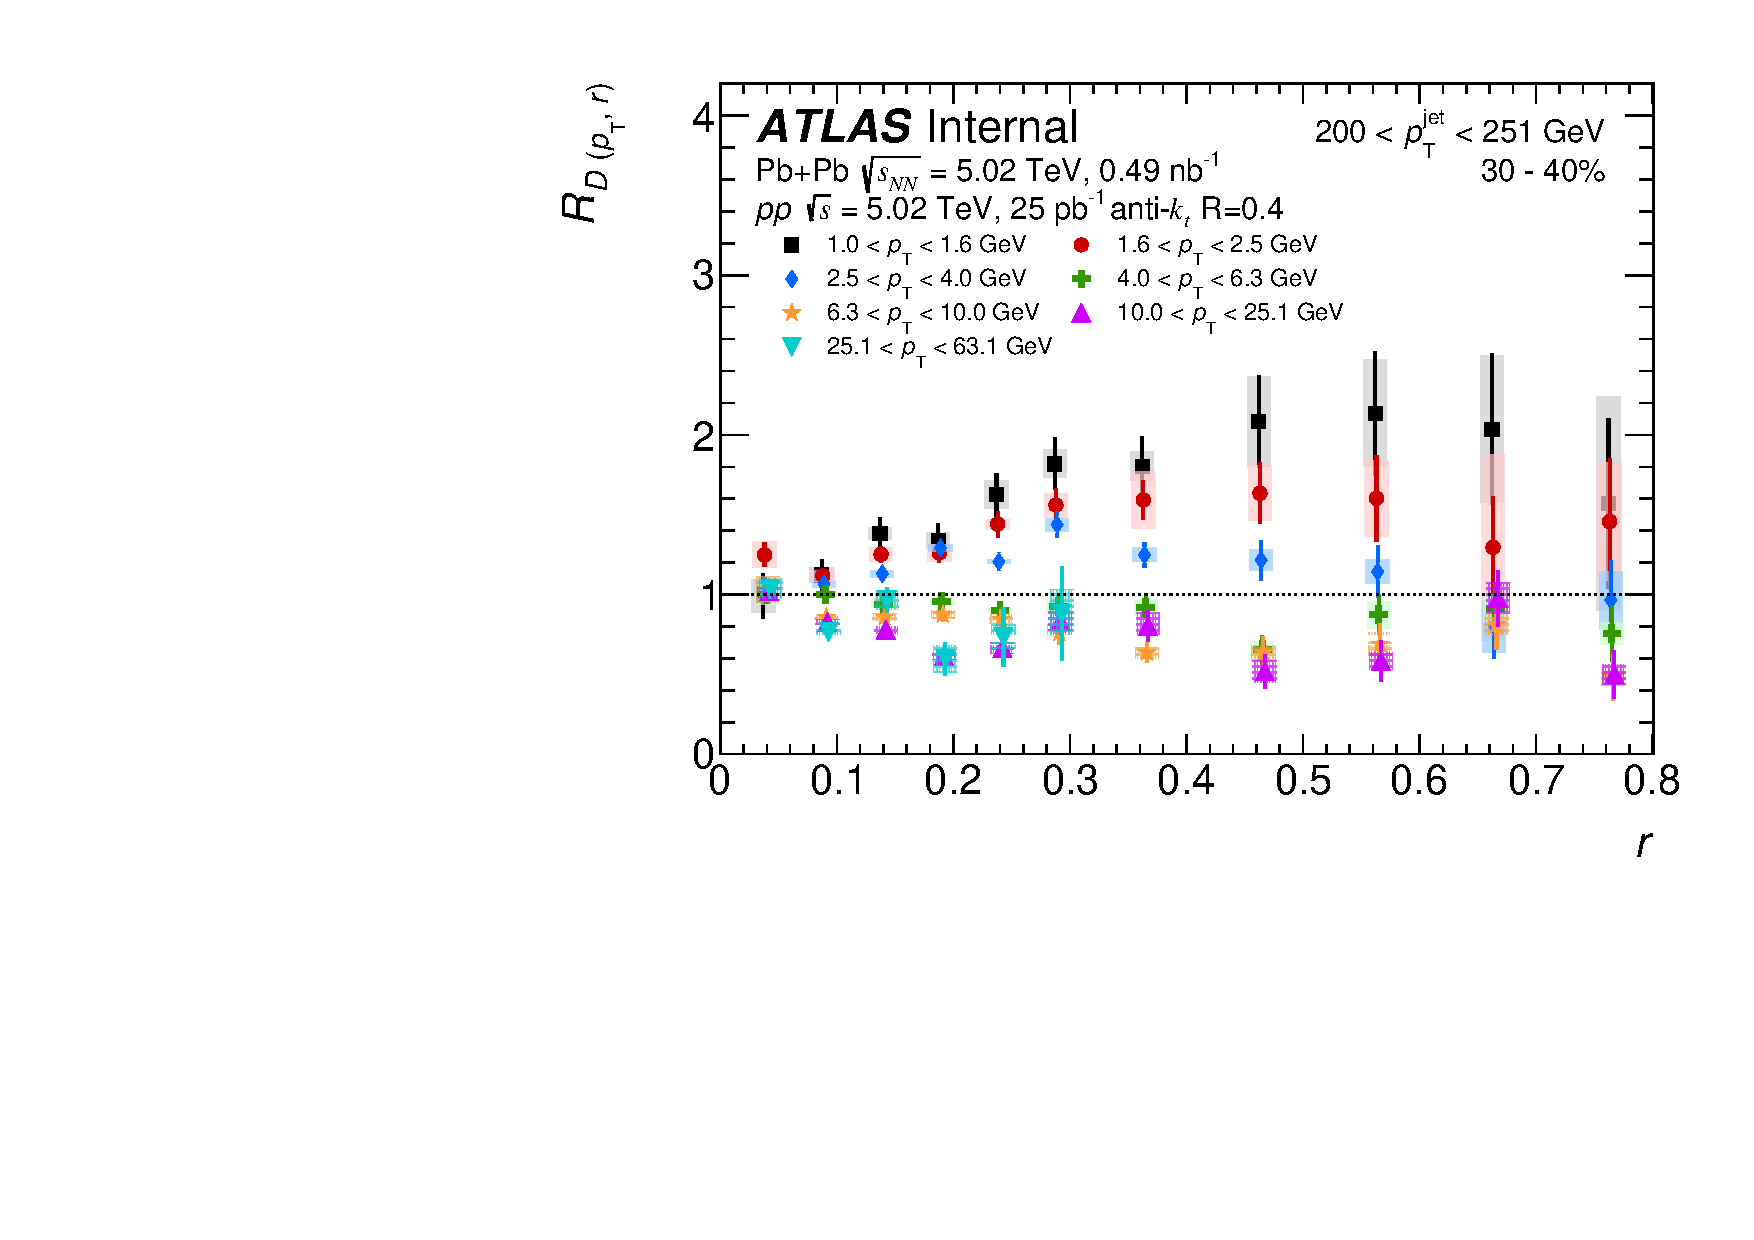
\includegraphics[width=0.5\textwidth]{figures/results/RDpT_dR_jet9_cent3.pdf} \\
            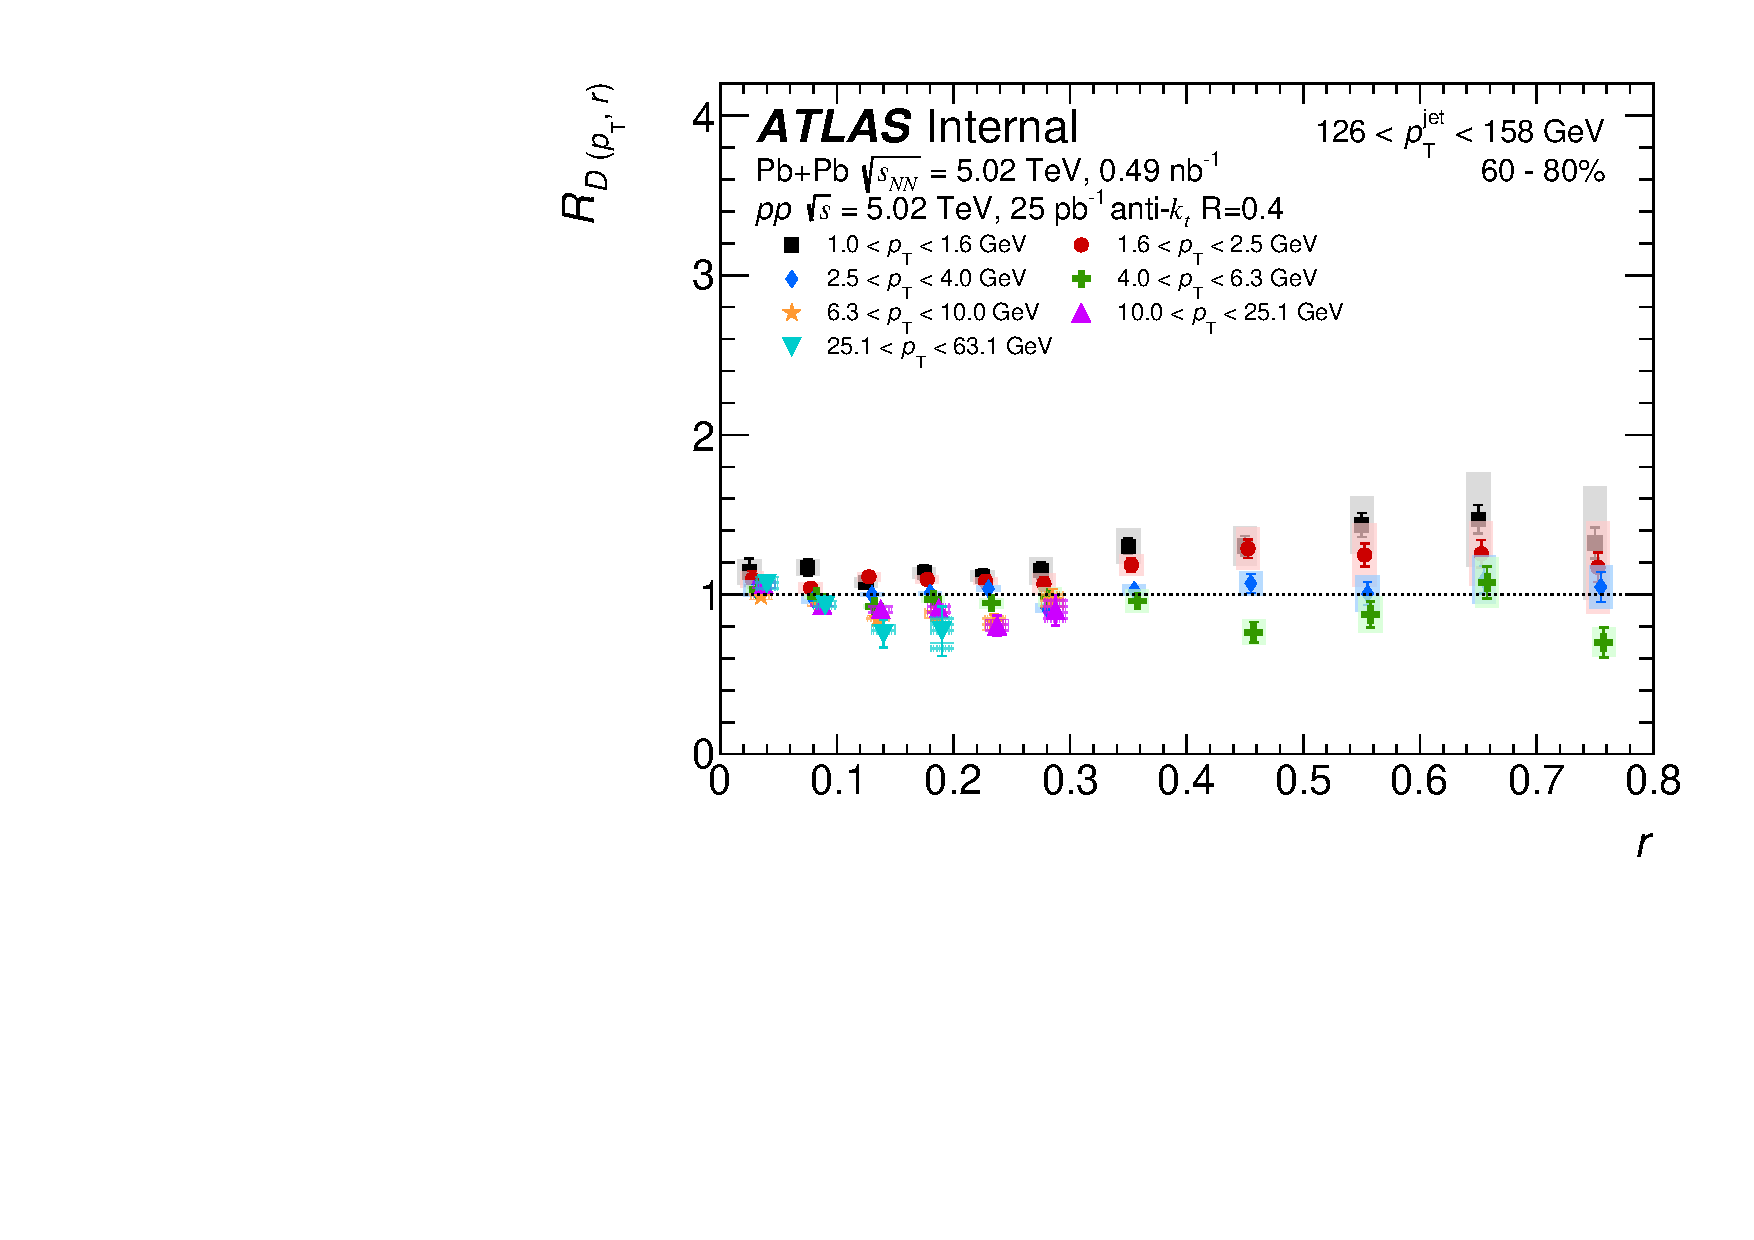
\includegraphics[width=0.5\textwidth]{figures/results/RDpT_dR_jet7_cent5.pdf} & 
            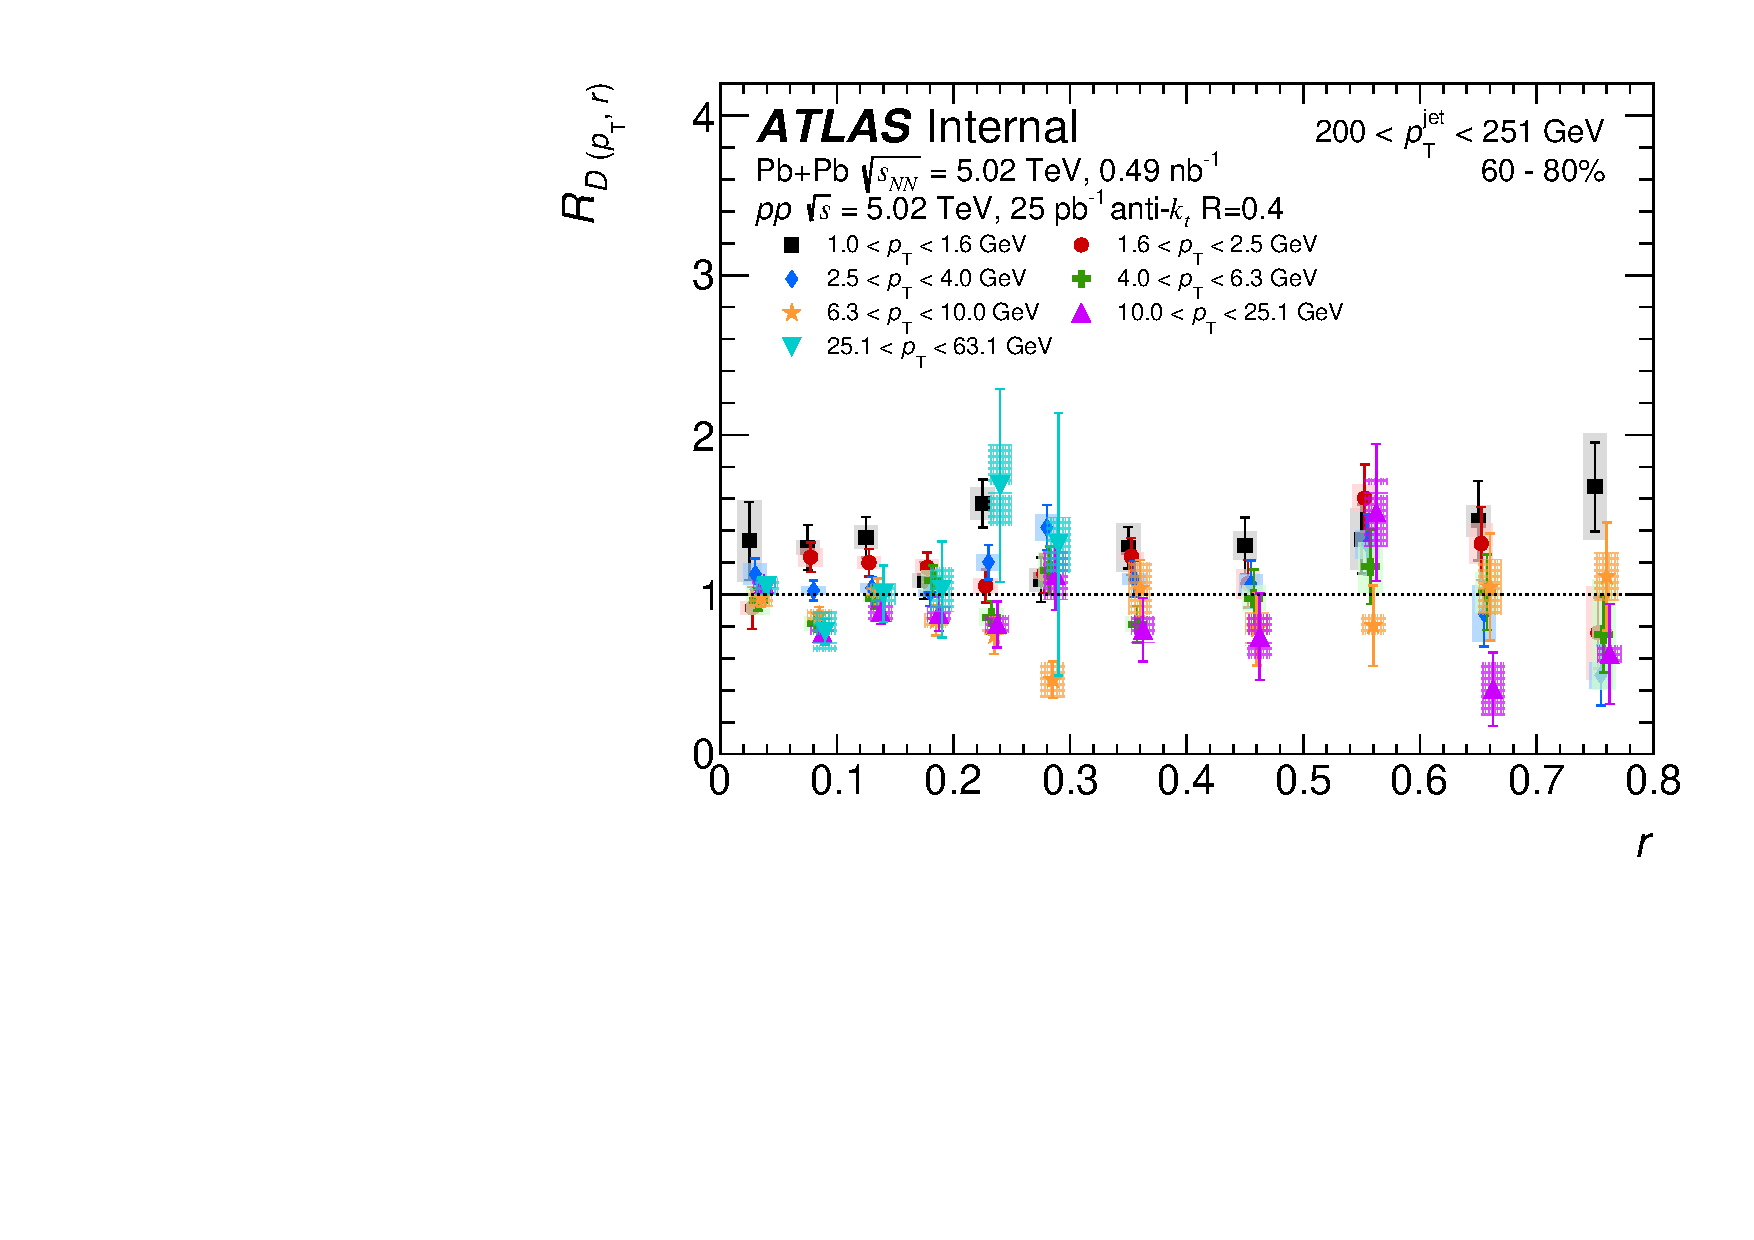
\includegraphics[width=0.5\textwidth]{figures/results/RDpT_dR_jet9_cent5.pdf} \\
      \end{tabular}
      }
\caption{Ratios of \Dptr\ distributions in 0--10\% (top), 30--40\% (middle), and 60--80\% (bottom) \PbPb\ collisions to \pp\ collisions as a function of angular distance $r$ for \ptjet\ of 126 to 158~\GeV\ (left) and of 200 to 251~\GeV\ (right) for six \pt\ selections. The vertical bars on the data points indicate statistical uncertainties while the shaded boxes indicate systematic uncertainties. The widths of the boxes are not indicative of the bin size and the points are shifted horizontally for better visibility.}
\label{fig:rdptr}
\end{figure}


% This observation is in agreement with the previous measurement of jet fragmentation functions \cite{Chatrchyan:2014ava, Sirunyan:2018jqr, Aaboud:2017bzv, PhysRevC.98.024908} and may indicate the dependence of the response of the hot dense matter to the momentum of a jet passing through it. 


\FloatBarrier

%-------------------------------------------------------------------------------
\section{Discussion}
\label{sec:discussion}
% !TEX root = trkjet.tex

%This section further discusses results from the previous section.

%%cent dependence
\subsection{\RDptr\ distributions}
Here the centrality, \ptjet\ and the charged-particle \pt\ depdendence of the \RDptr\ distributions introduced in 
Section~\ref{sec:results} are discussed.

\begin{figure}[ht]
\centerline{
         \begin{tabular}{cc}
%            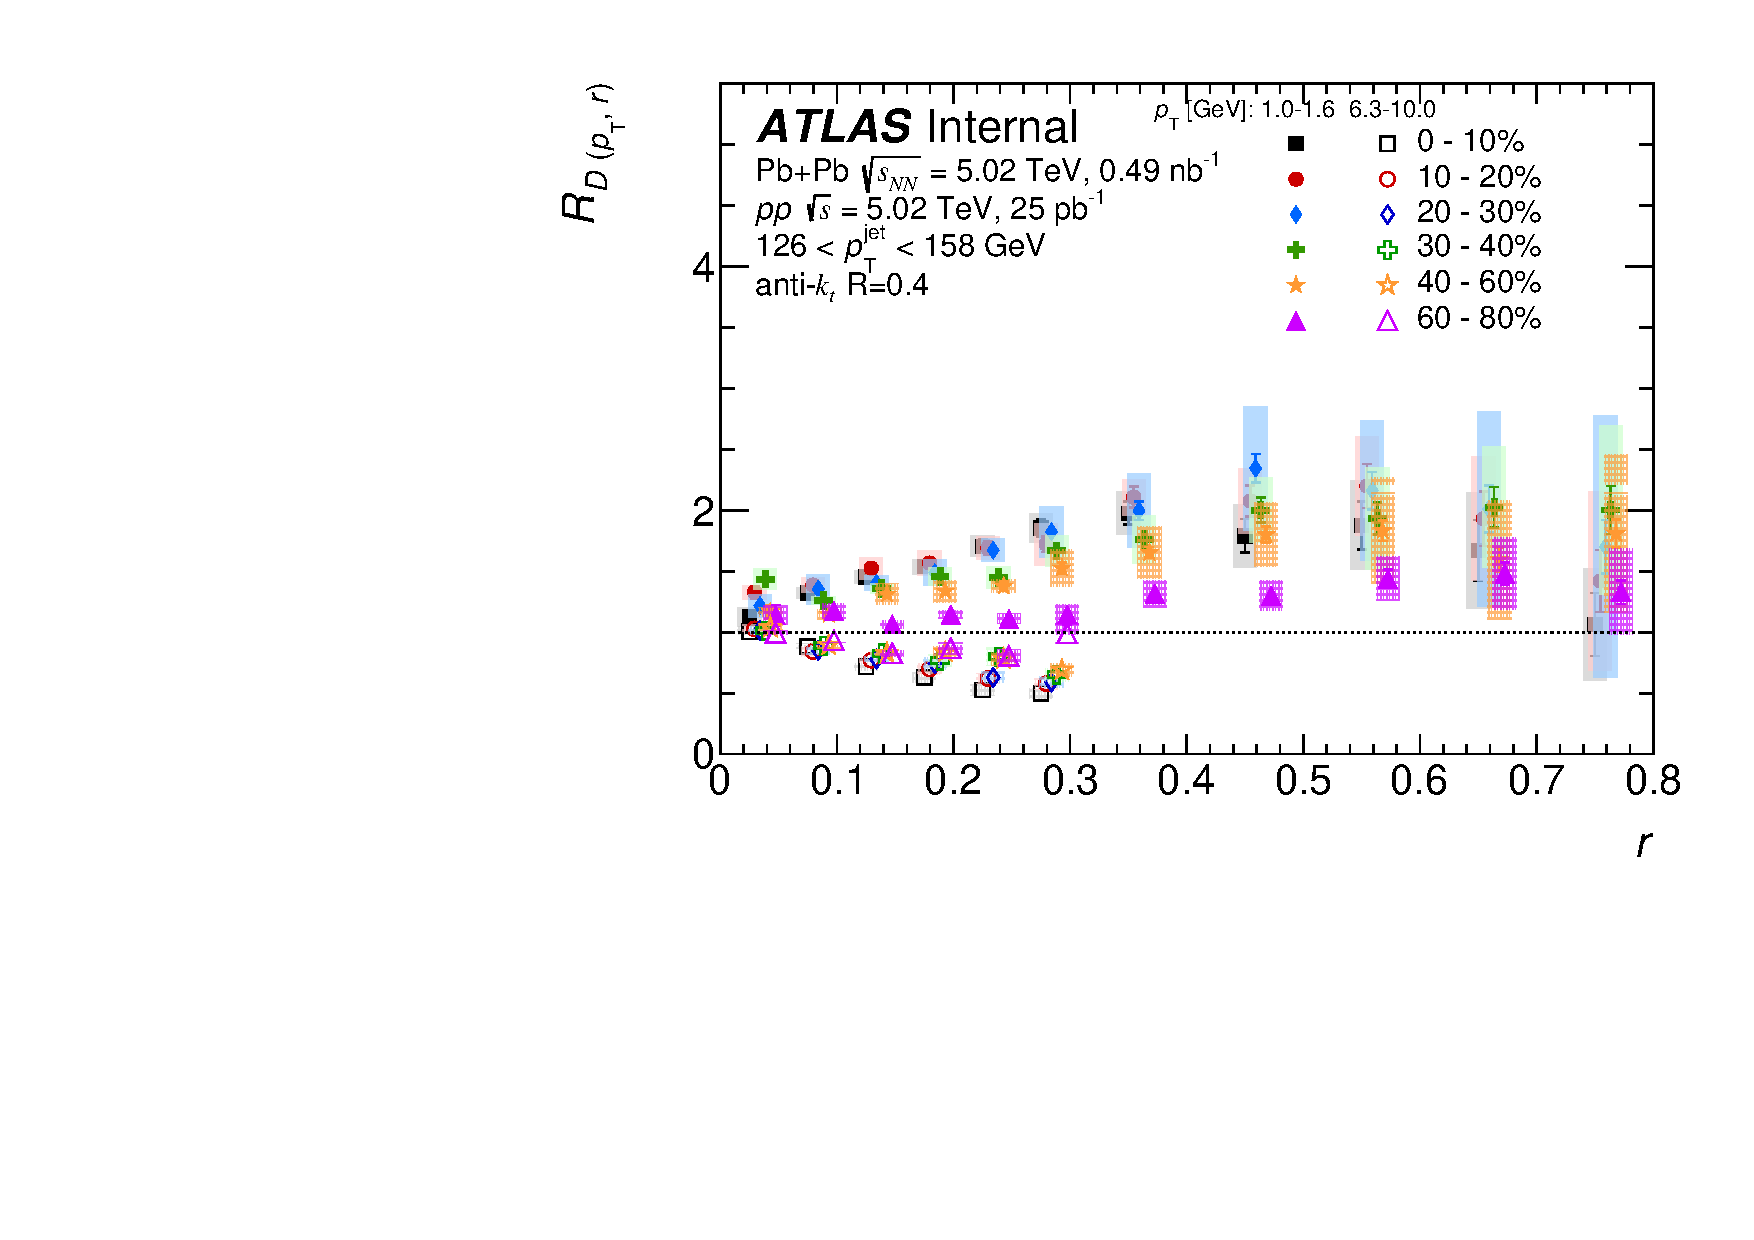
\includegraphics[width=0.5\textwidth]{figures/results/RDpT_dR_trk2_trk6_jet7.pdf} & 
%            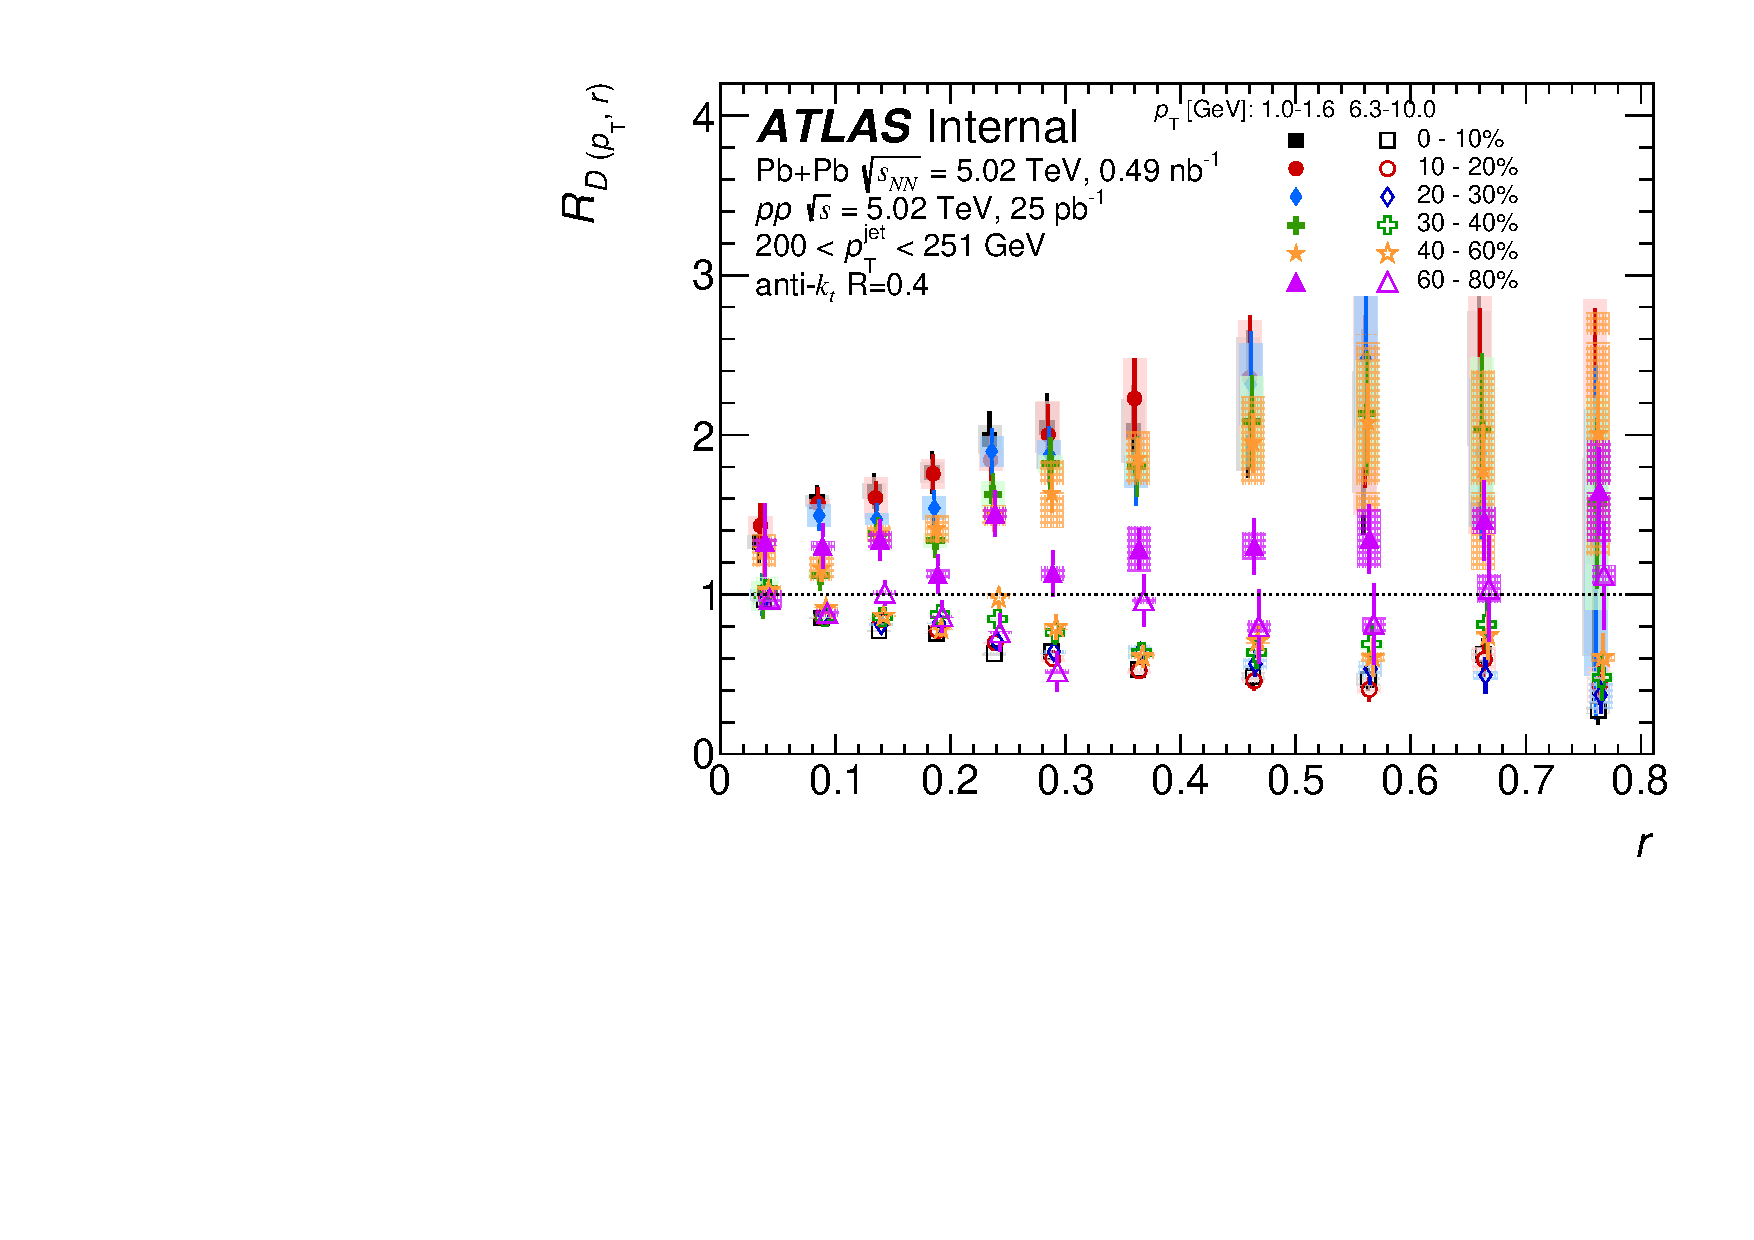
\includegraphics[width=0.5\textwidth]{figures/results/RDpT_dR_trk2_trk6_jet9.pdf} \\
            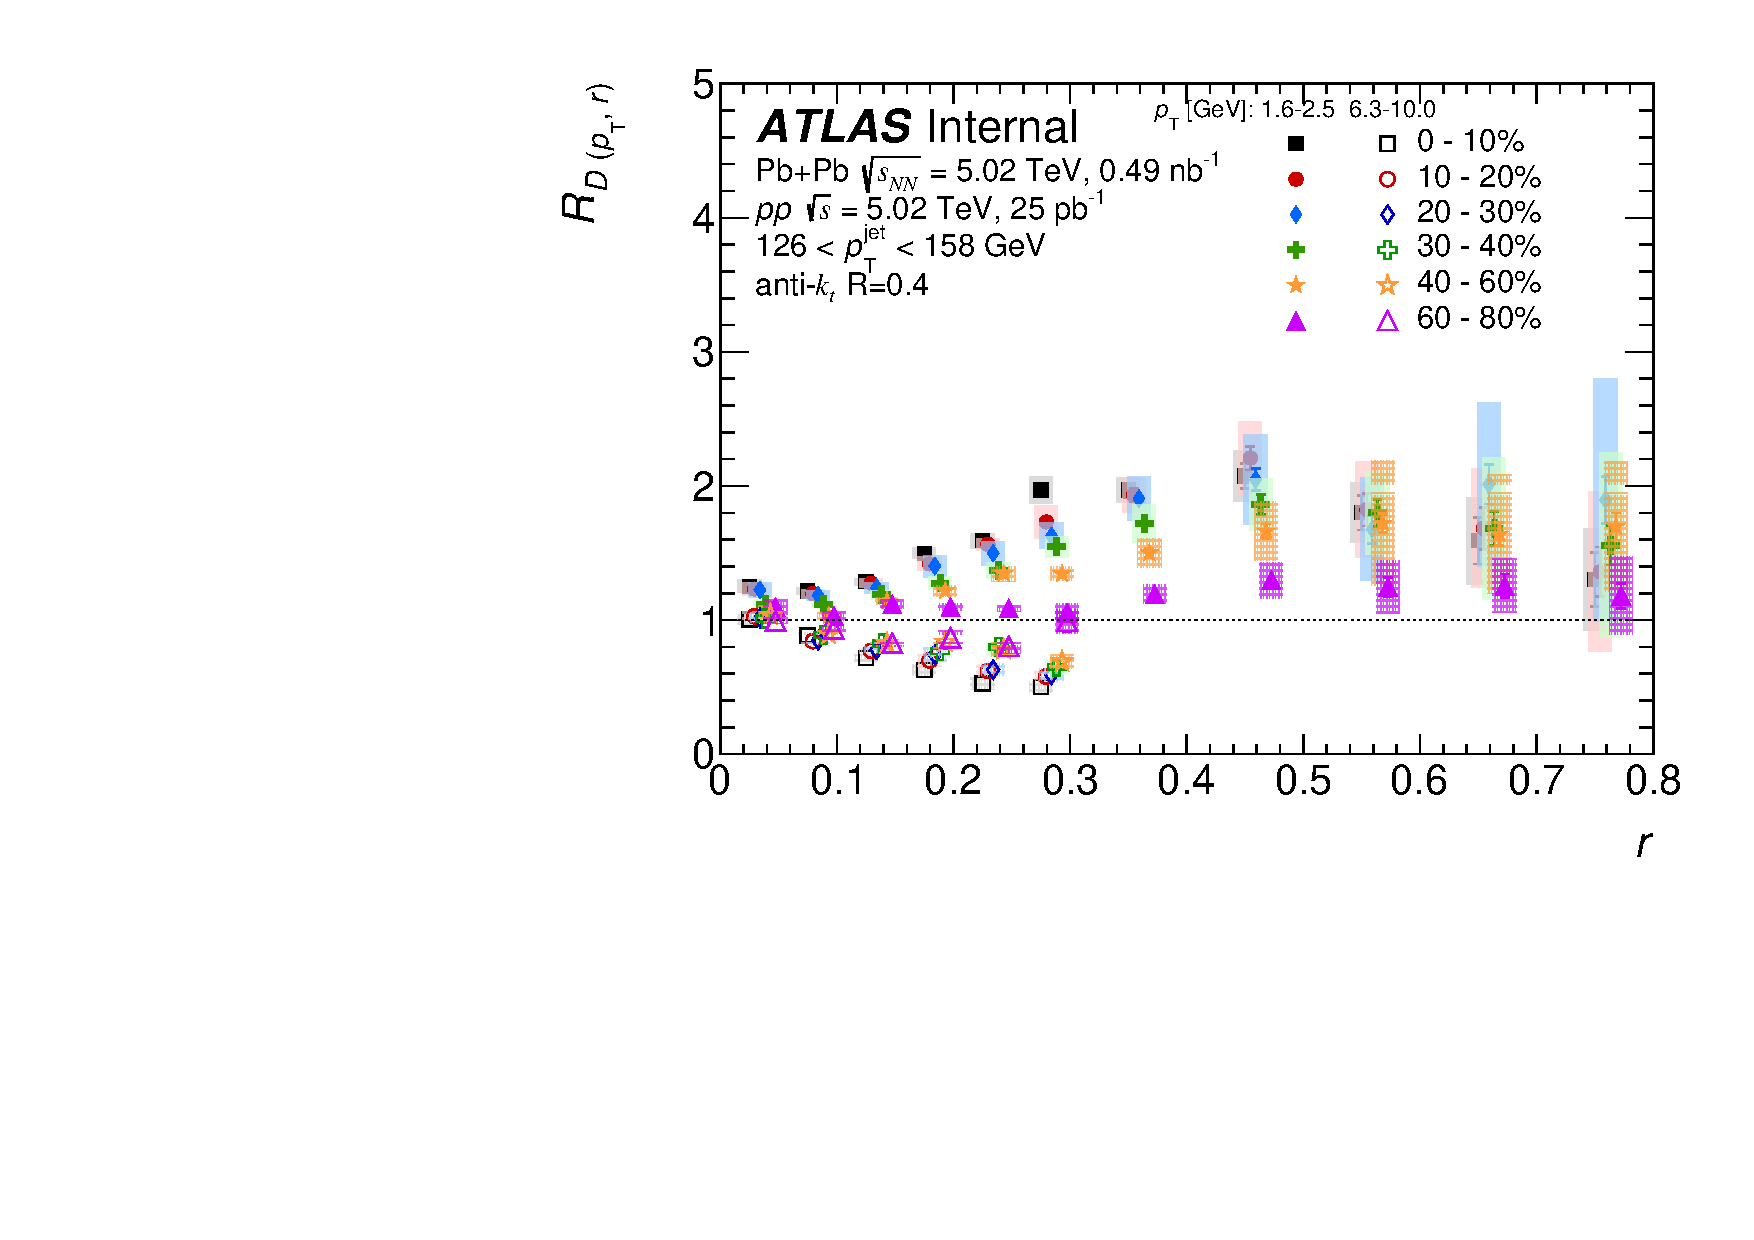
\includegraphics[width=0.5\textwidth]{figures/results/RDpT_dR_trk3_trk6_jet7.pdf} & 
            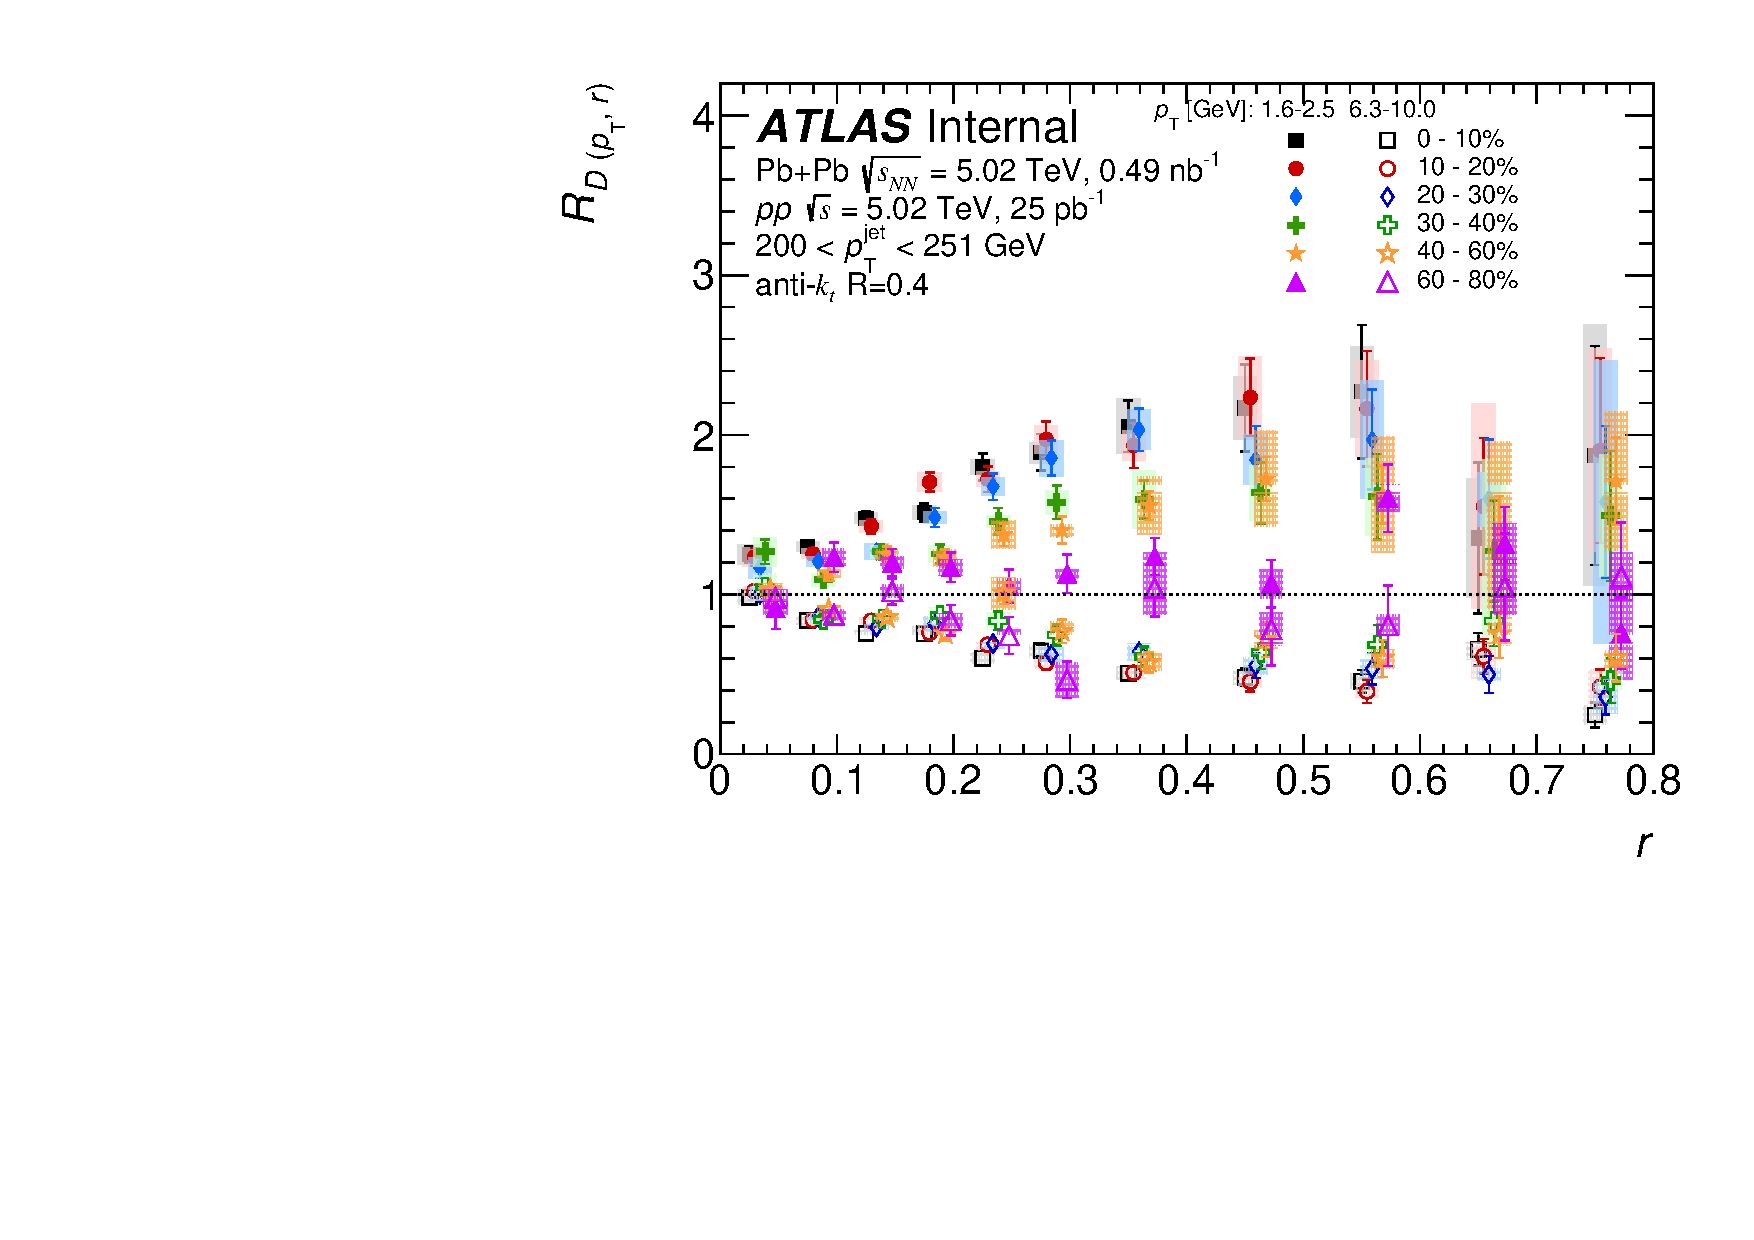
\includegraphics[width=0.5\textwidth]{figures/results/RDpT_dR_trk3_trk6_jet9.pdf} \\
      \end{tabular}
      }
   \caption{The \RDptr\ distributions for \ptjet\ of 126--158~\GeV\ and 200--251~\GeV\ as a function of angular distance $r$ for two \pt\ selections, 1.6--2.5~\GeV\ (closed symbols) and 6.3--10.0~\GeV\ (open symbols), and six centrality intervals. The vertical bars on the data points indicate statistical uncertainties while the shaded boxes indicate systematic uncertainties. The widths of the boxes are not indicative of the bin size and the points are shifted horizontally for better visibility.}
\label{fig:centdep}
\end{figure}
%%%%%%%%%%%%%

The centrality dependence of \RDptr\ for two charged-particle \pt\ intervals: 1.6--2.5~\GeV\ and \mbox{6.3--10.0~\GeV}, and two different \ptjet\ ranges: 126--158~\GeV\ and 200--251~\GeV, is presented in Figure~\ref{fig:centdep}. 
For both \ptjet\ selections and  1.6--2.5~\GeV\ charged particles, the magnitude of the excess increases
with increasing collision centrality and \rvar\ for $\rvar < 0.3$.  The magnitude of the excess is
approximately a factor of two in the most central collisions for $\rvar >$~0.3.
A continuous centrality dependent suppression of  yields of charged-particles with $6.3 < \pt < 10.0$ GeV is observed.
%With the same \ptjet\ selections and 
%charged-particles with 6.3~$ < \pt < $~10.0~\GeV a clear ordering in centrality is observed with
%the most central collisions exhibiting the smallest \RDptr\ values.
The magnitude of the modifications decreases with decreasing collision centrality for both \pt\ 
intervals and \ptjet\ selections.

\begin{figure}[ht]
\centerline{
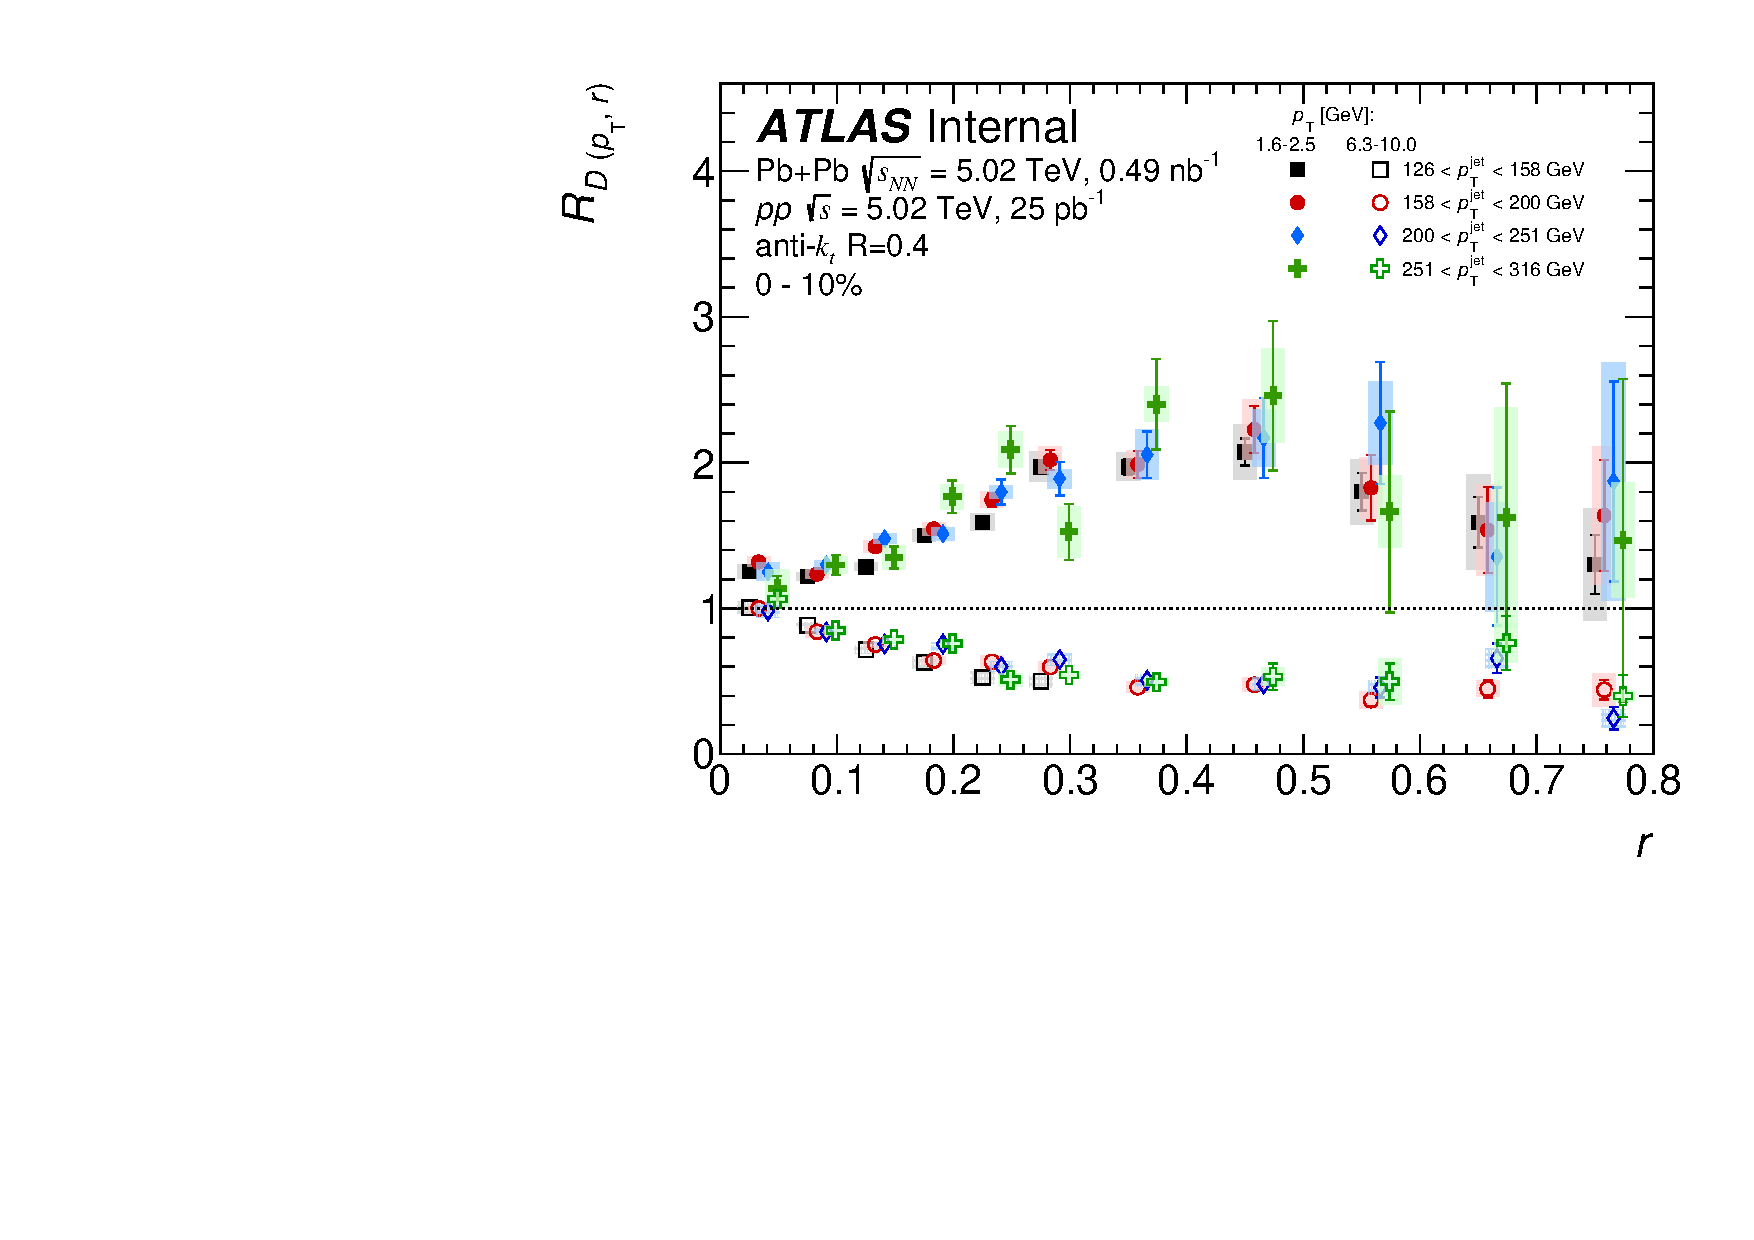
\includegraphics[width=0.8\textwidth]{figures/results/RDpT_dR_trk3_trk6_cent0.pdf} 
}
\caption{\RDptr\ as a function of \rvar\ for 0--10\% collisions for charged particles with 1.0~$< \pt <$~1.6~\GeV\
(closed symbols) and 6.3~$< \pt <$10.0~\GeV\ (open symbols) for different \ptjet\ selections. The vertical bars on the data points indicate statistical uncertainties while the shaded boxes indicate systematic uncertainties. The widths of the boxes are not indicative of the bin size and the points are shifted horizontally for better visibility.}
\label{fig:ptjetdep}
\end{figure}
%%%%%%%%%%%%%


%In order to directly explore the \ptjet\ dependence of \RDptr\, the values are overlaid for all four
%\ptjet\ selections measured here in Figure~\ref{fig:ptjetdep} for the 0--10\% most central collisions 
%and the same two charged-particle \pt\ selections as in Figure~\ref{fig:centdep}.
The \RDptr\ distributions for low and high \pt\ particles in the different \ptjet\ selections are directly overlaid in Figure~\ref{fig:ptjetdep}. These distributions are for the 0--10\% 
most central collisions, and suggest an increasing \ptjet\  for $r < 0.25$ for low 
\pt\ charged particles. No significant \ptjet\ dependence is seen at larger \rvar\ values. Furthermore, the \RDptr\ distributions for high-\pt\ charged particles do not seem to show any significant \ptjet\ dependence at any \rvar.


\begin{figure}
\centering{
\begin{tabular}{cc}
	 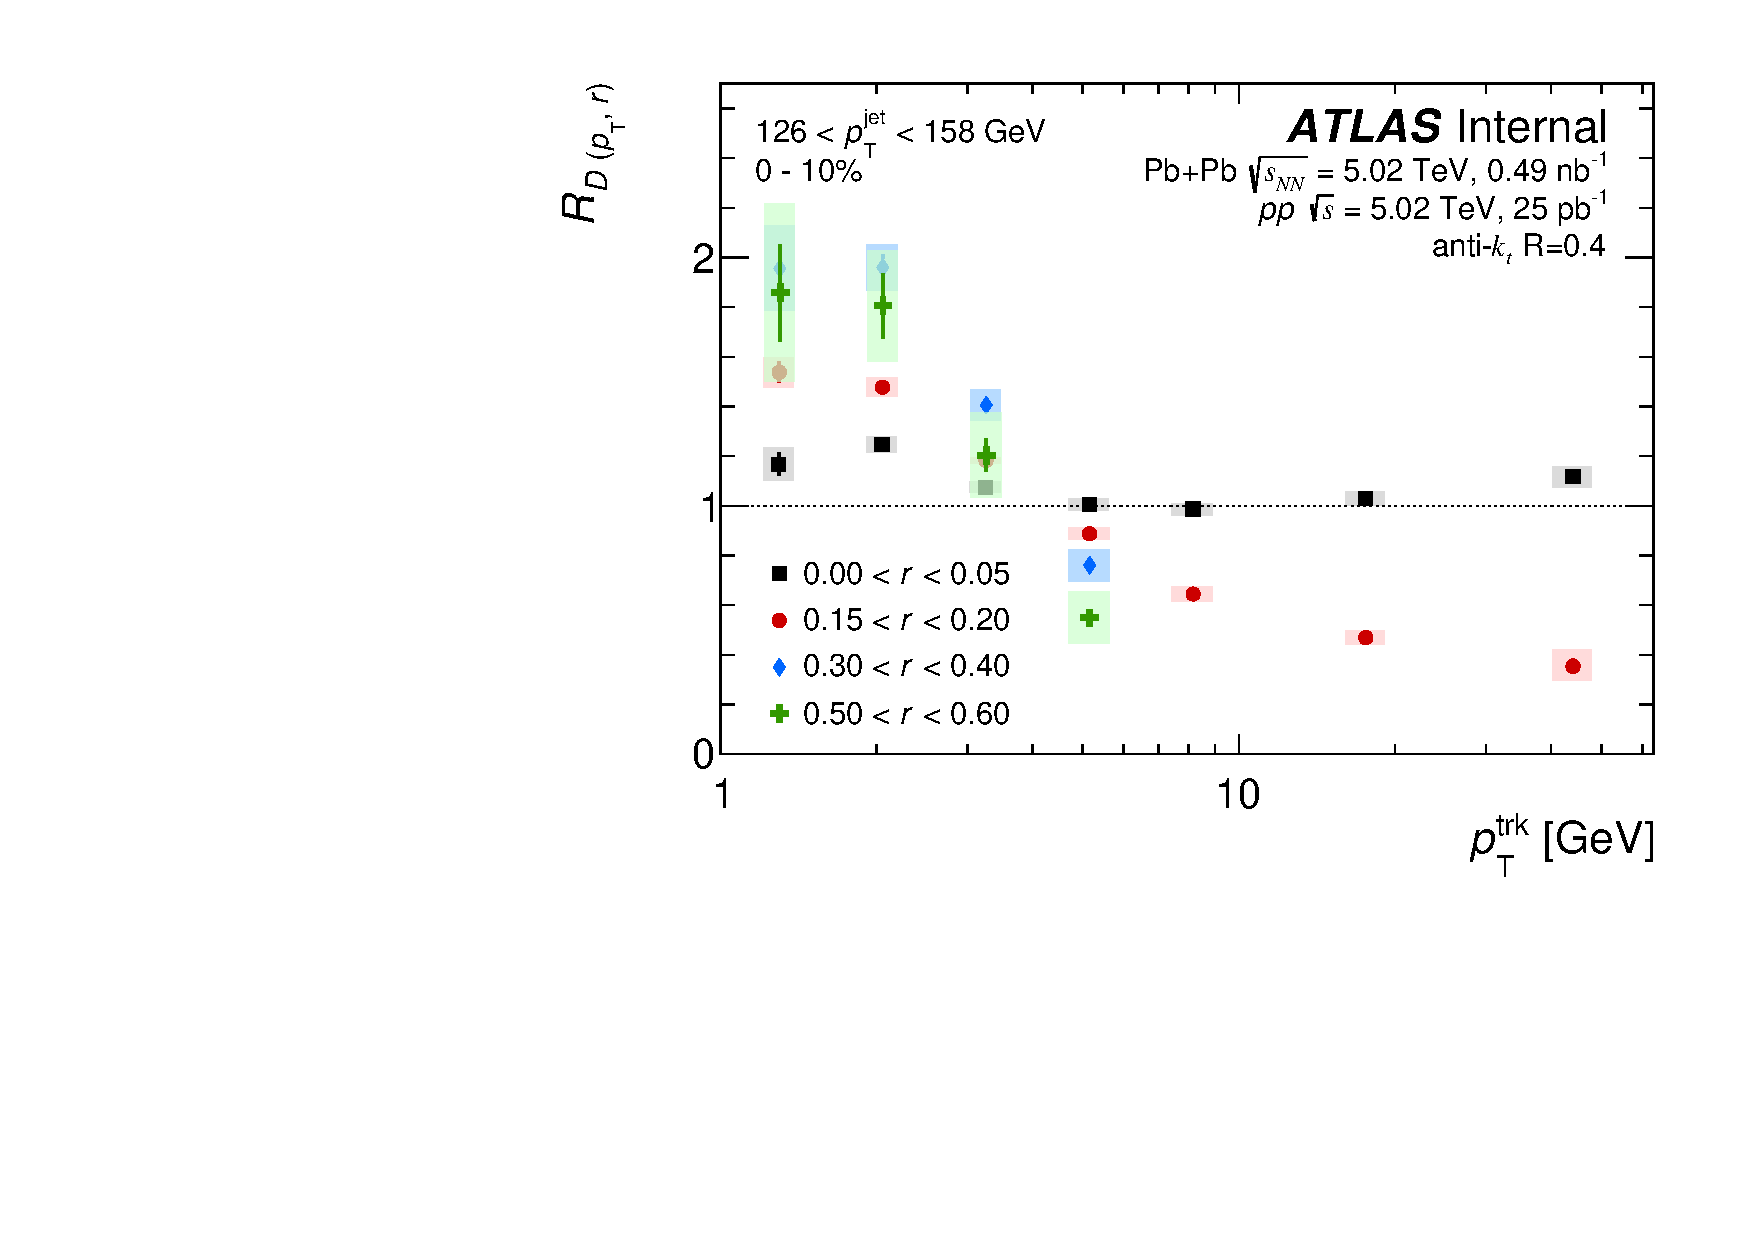
\includegraphics[width=0.5\textwidth]{results/RDpT_trkpt_jet7_cent0} &
	 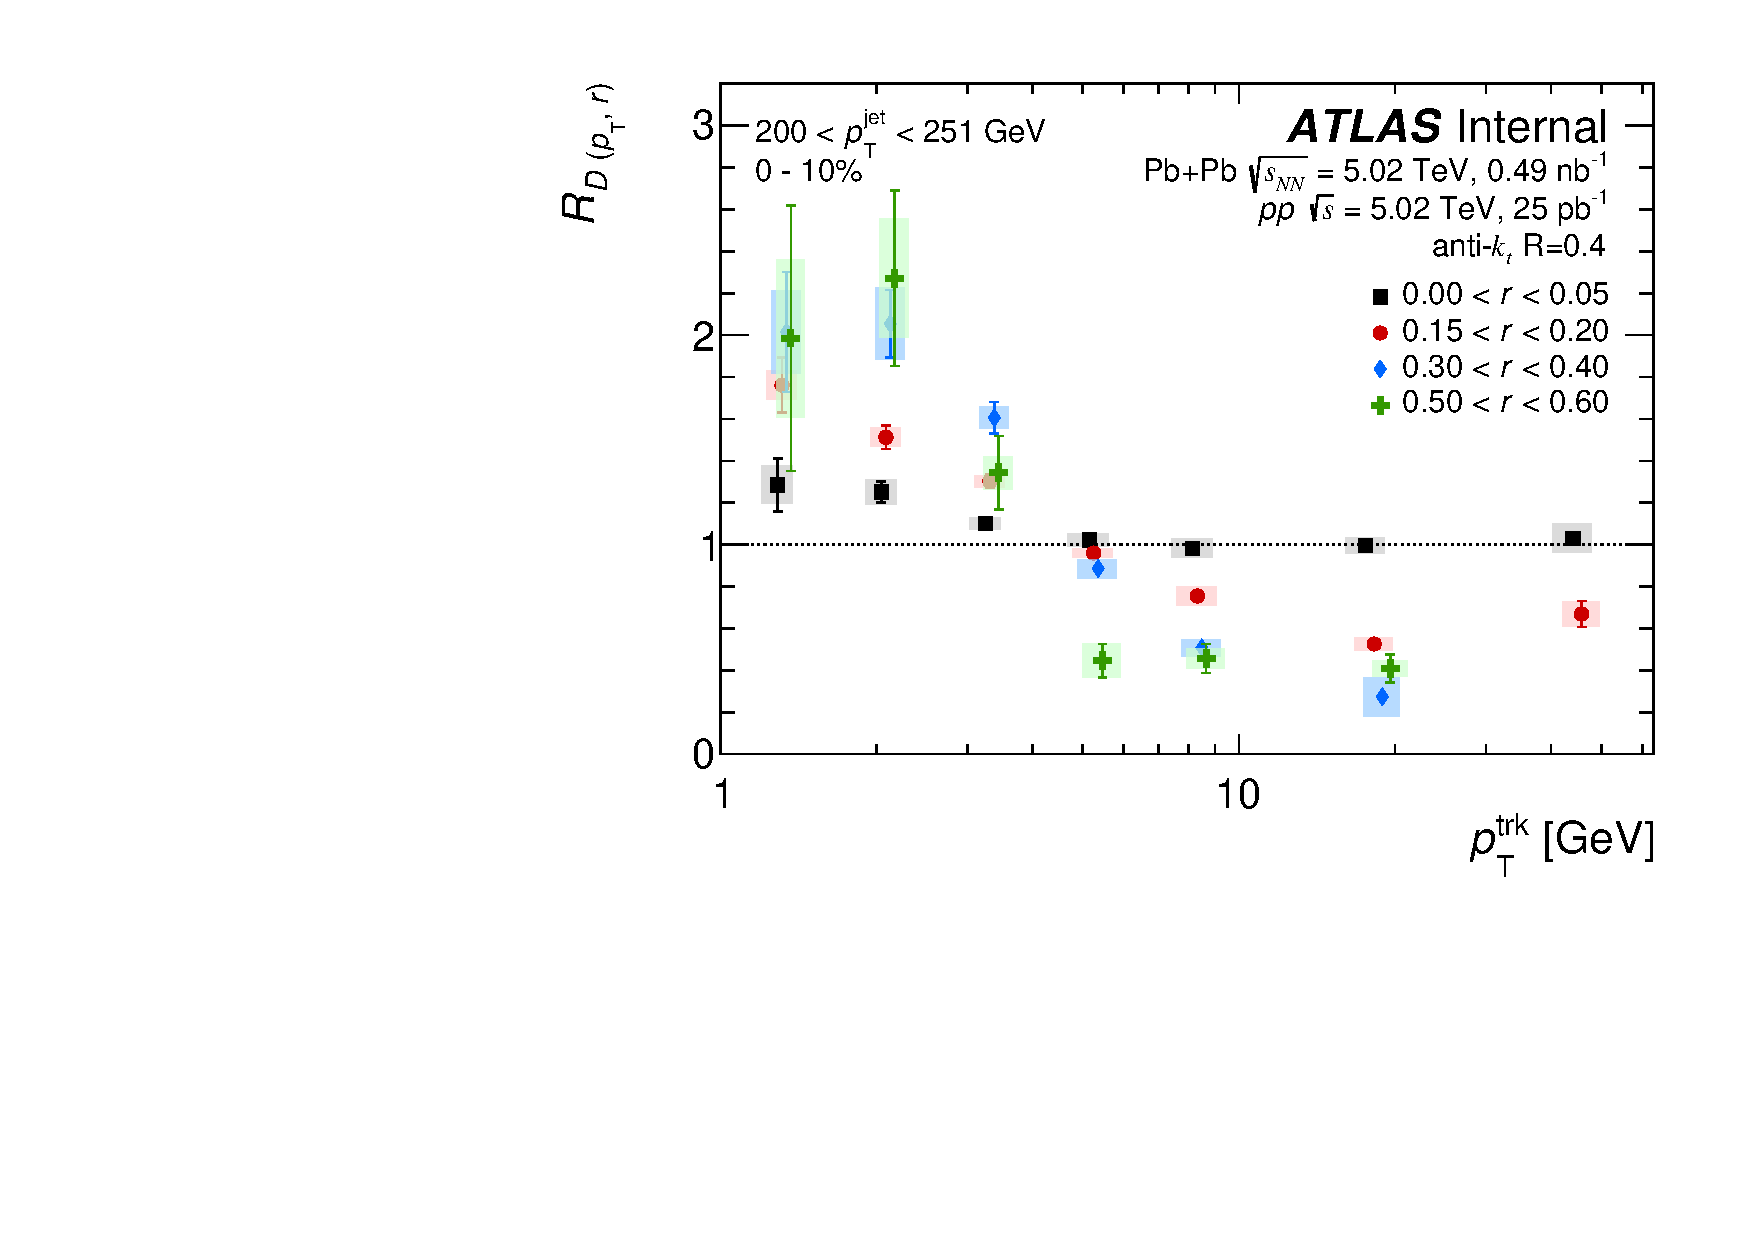
\includegraphics[width=0.5\textwidth]{results/RDpT_trkpt_jet9_cent0} \\
	 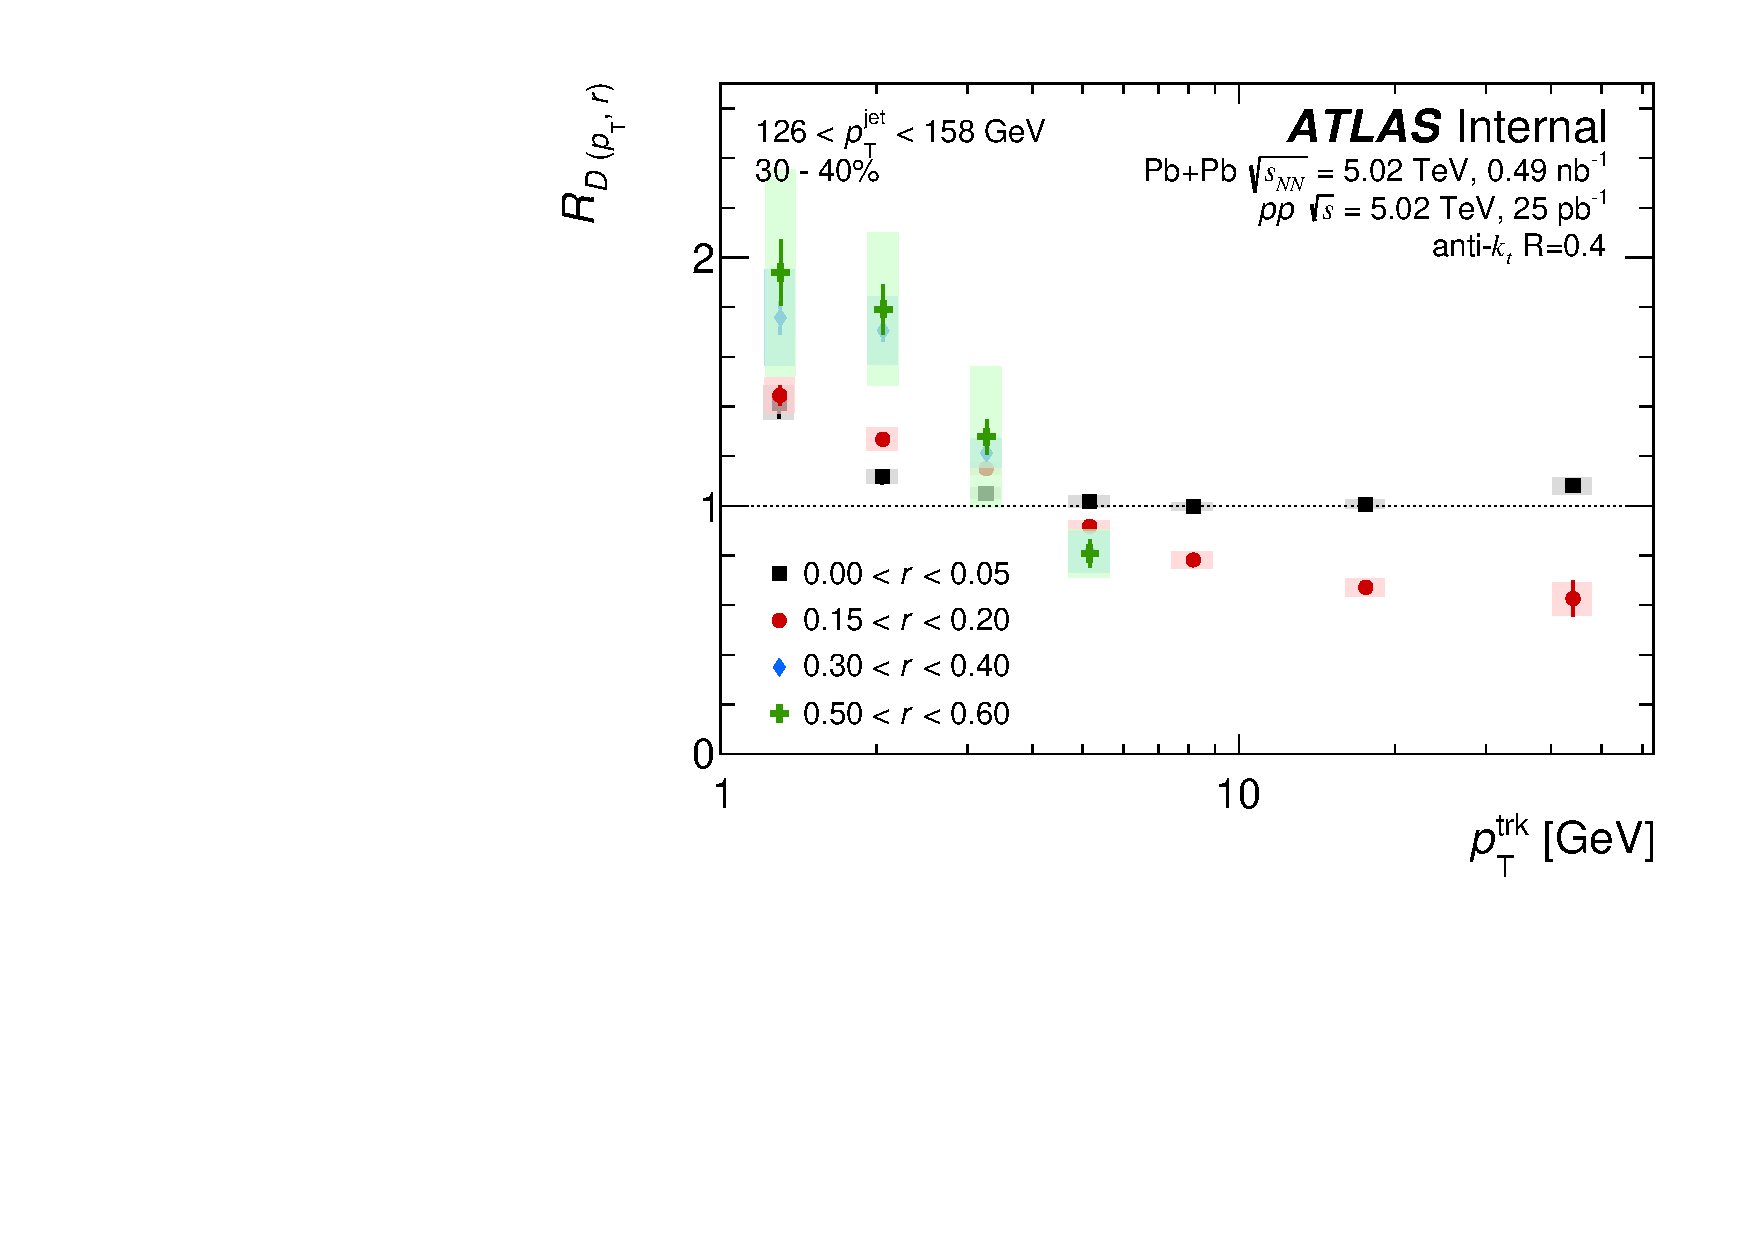
\includegraphics[width=0.5\textwidth]{results/RDpT_trkpt_jet7_cent3} &
	 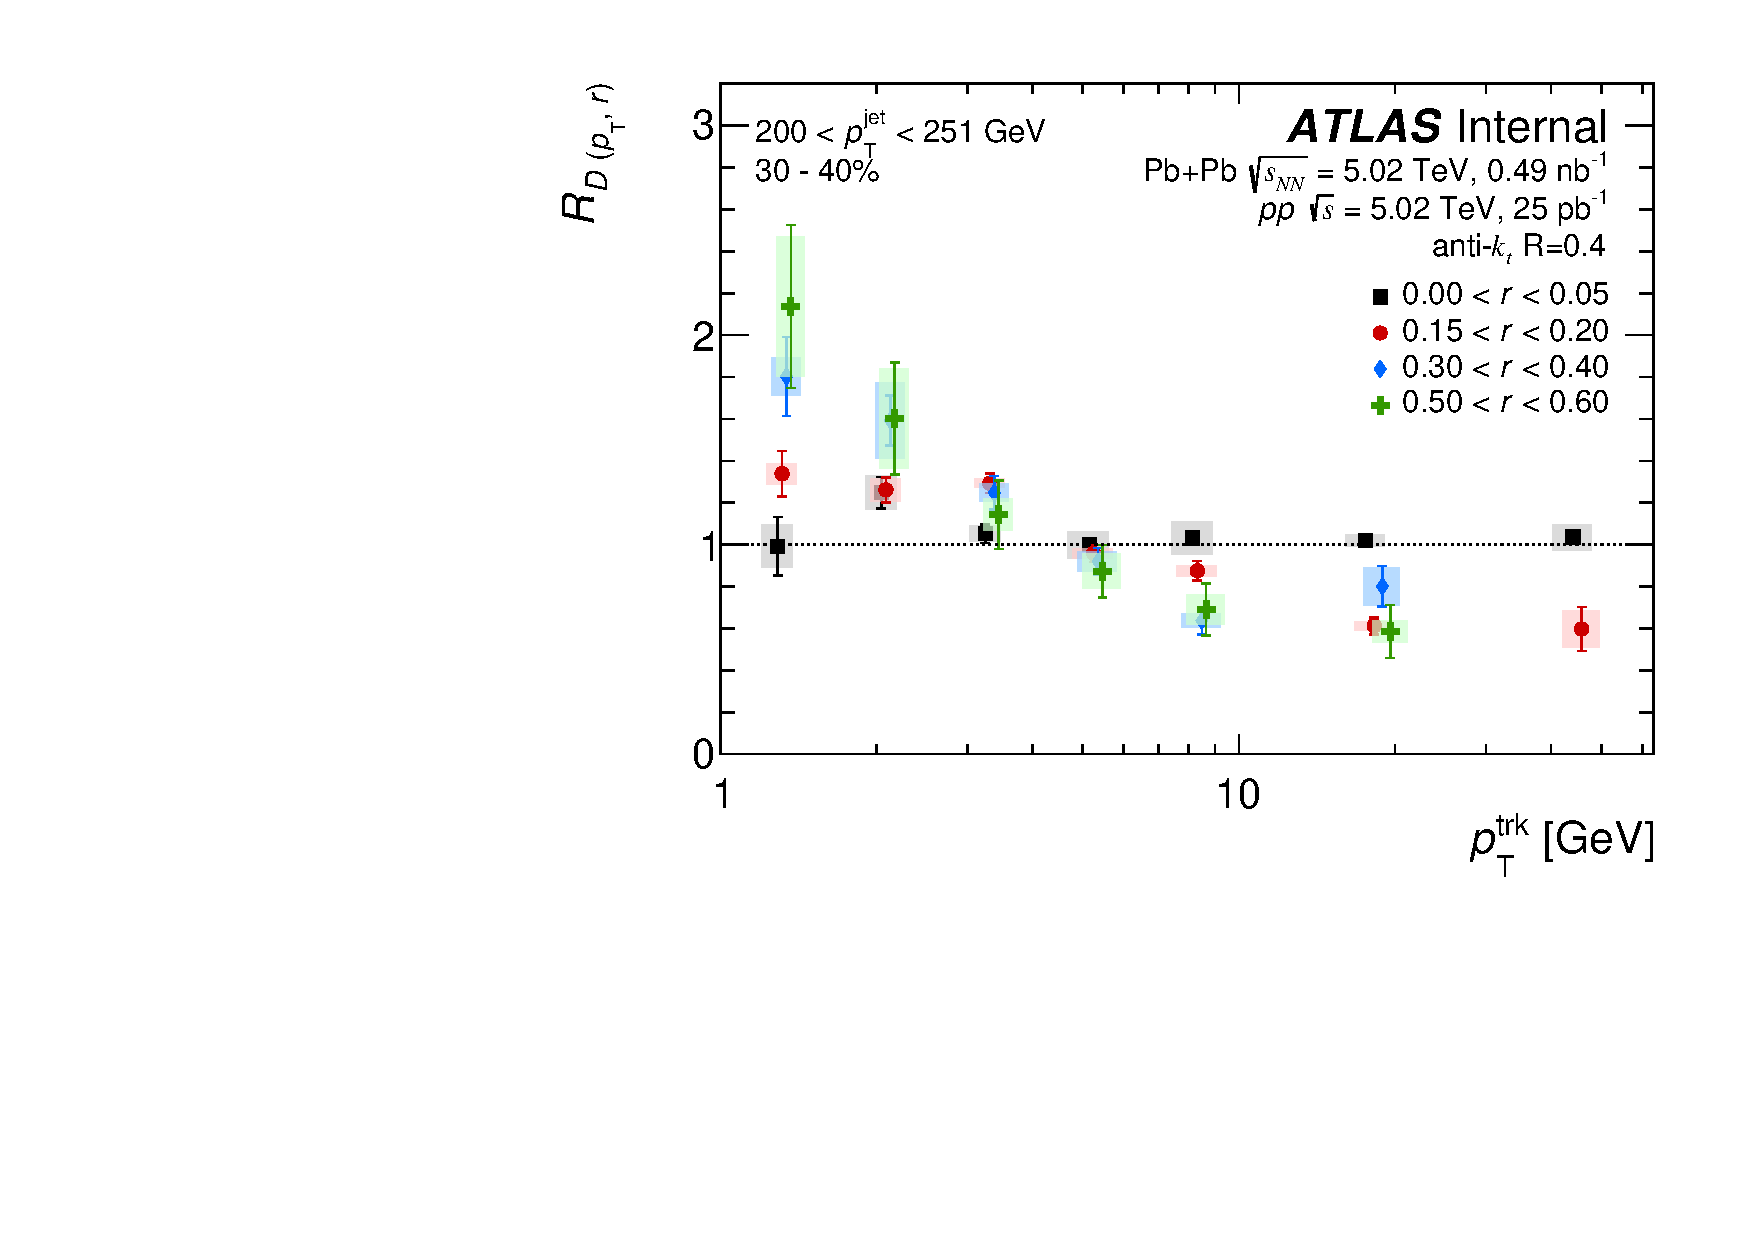
\includegraphics[width=0.5\textwidth]{results/RDpT_trkpt_jet9_cent3} \\
	 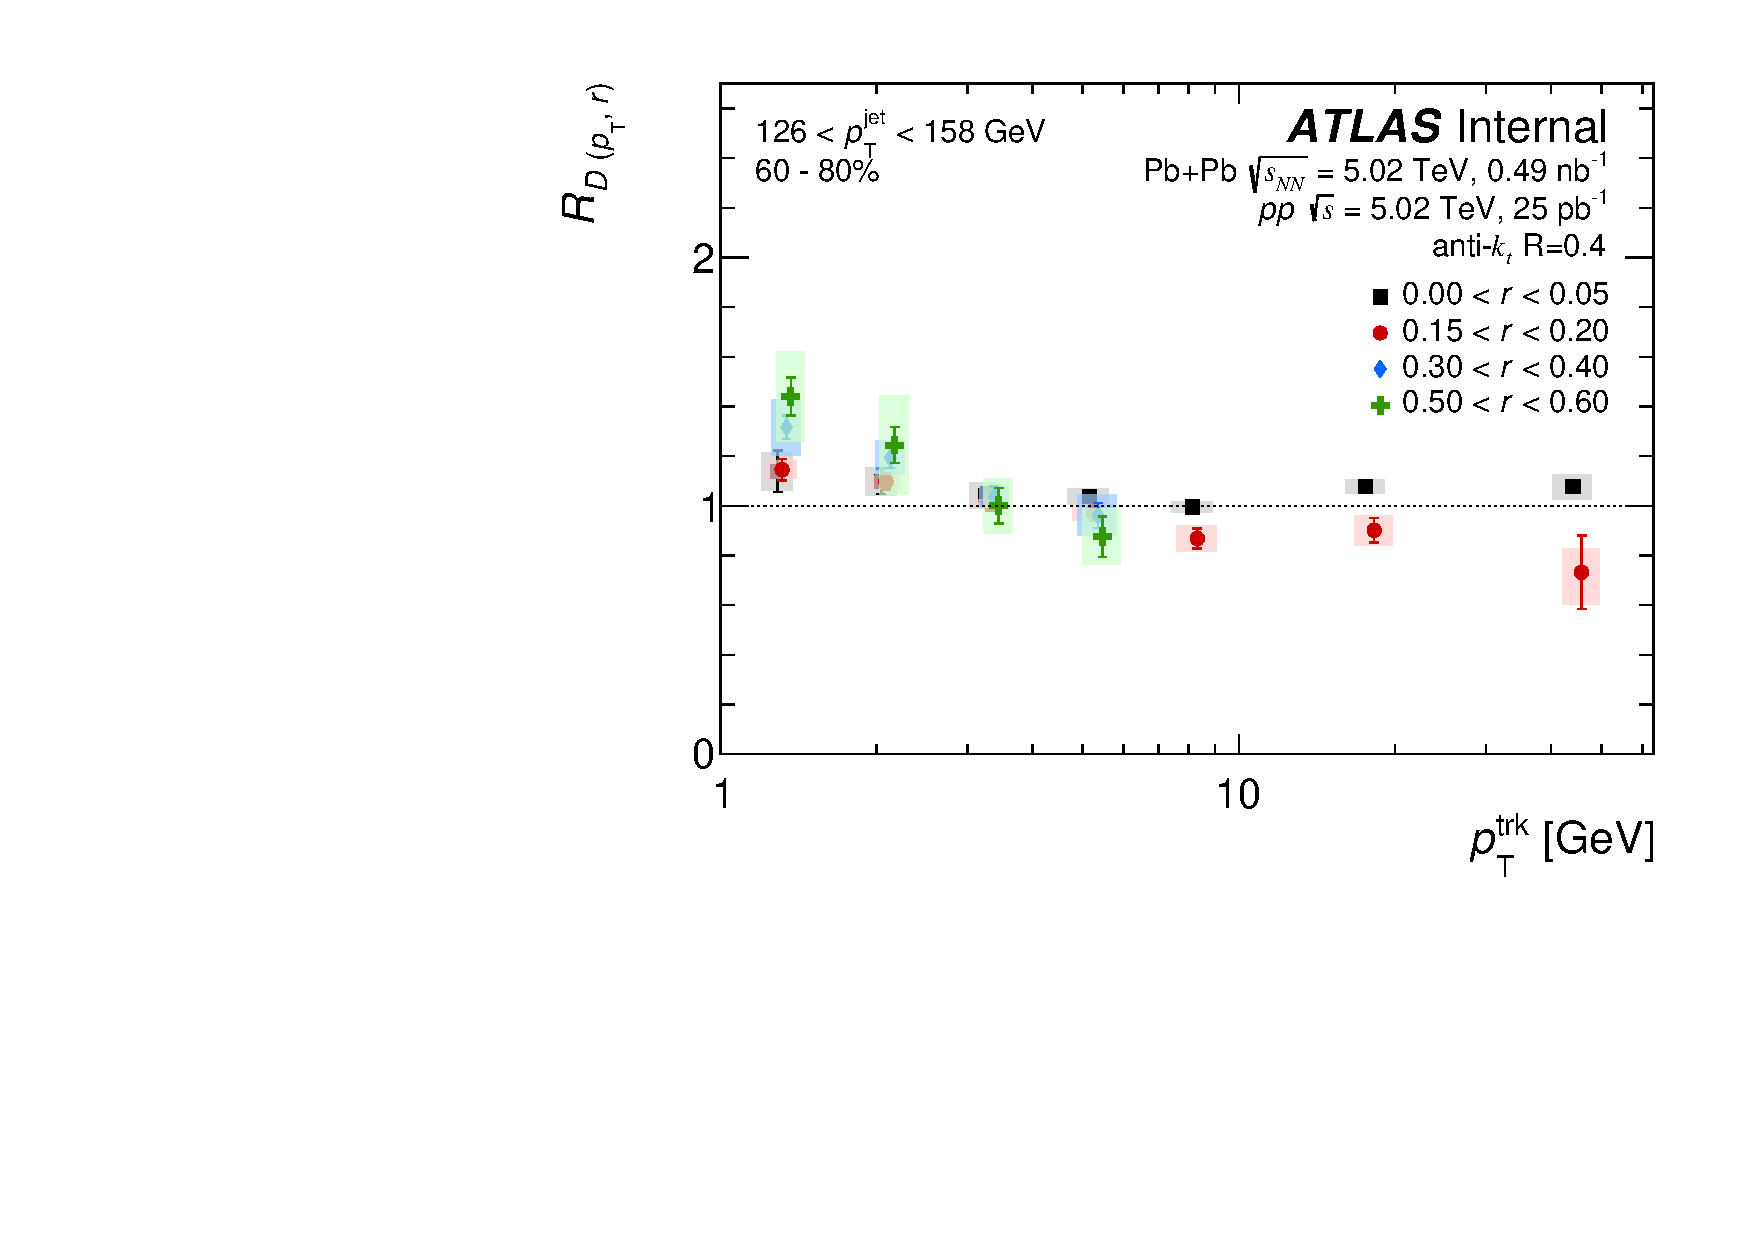
\includegraphics[width=0.5\textwidth]{results/RDpT_trkpt_jet7_cent5} &
	 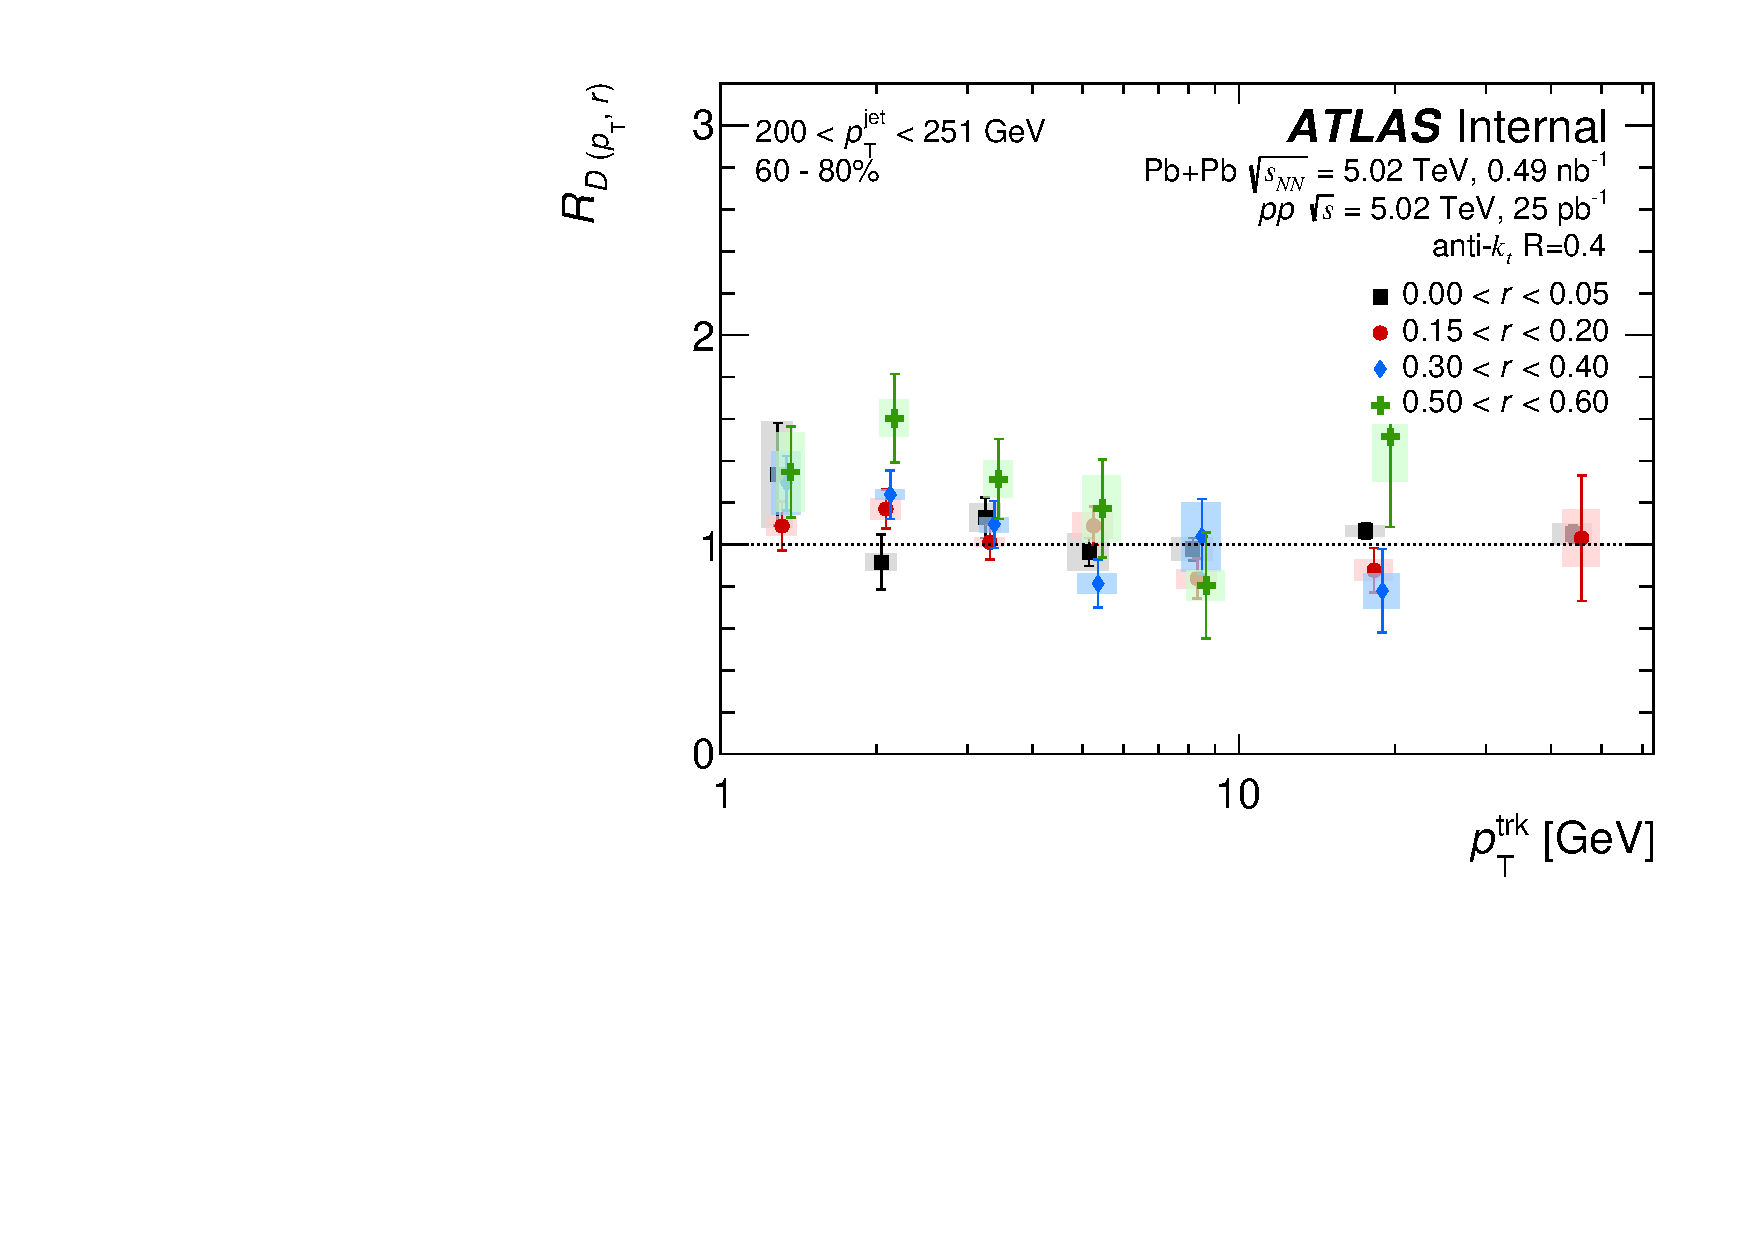
\includegraphics[width=0.5\textwidth]{results/RDpT_trkpt_jet9_cent5} \\
\end{tabular} }
   \caption{\RDptr\ as a function of \pt\ in  0--10\% (top), 30--40\% (middle), and 60--80\% (bottom) \PbPb\ collisions to \pp\ collisions for two different \ptjet\ selections: 126--158~\GeV\ (left) and 200--251~\GeV\ (right). The different colors indicate different angular distances from the jet axis. The vertical bars on the data points indicate statistical uncertainties while the shaded boxes indicate systematic uncertainties. The widths of the boxes are not indicative of the bin size and the points are shifted horizontally for better visibility.}
      \label{fig:pttrkdep}
\end{figure}


%%pt track dependence
In Figure~\ref{fig:rdptr}, it was shown that for central and mid-central collisions, there is an enhancement of
charged particles with $\pt <$~4.0~\GeV\ and a suppression of charged particles with $\pt >$~4.0~\GeV.  In
Figure~\ref{fig:pttrkdep} 
the \pt\ dependance for selections in \rvar\ is directly investigated for 0--10\%, 30--40\% and 60--80\% central 
collisions for 126--158 GeV and 200--251~\GeV\ jets.
Interestingly, at all measured \pt, there is no significant suppression of the yields in \pbpb\ collisions
for $\rvar < 0.05$.  For larger \rvar\ values the yields are enhanced for charged-particles with $\pt <$~4~\GeV\ and 
suppressed for higher \pt\ charged-particles in both the 0--10\% and 30--40\% centrality selections and both \ptjet\ 
ranges presented here.  The magnitude of the enhancement increases for decreasing \pt\ at low \pt, while the suppression is enhanced
with increasing \pt at high \pt, until about 10~\GeV, after which it is approximately constant.
At fixed \pt\ the magnitude of the deviation from unity is largest for $0.3< \rvar < 0.4$ and $0.5< \rvar < 0.6$.
In the 60--80\% central collisions, the same trend remains true (but with smaller magnitude 
modifications) for \mbox{$126 < \ptjet < 158$ GeV}; for the higher \ptjet\ selection the larger uncertainties 
do not allow a clear conclusion to be drawn for peripheral collisions.

One possible explanation of the modification of the 
jet fragmentation in the kinematic region of $\pt > 4$ GeV range is the larger expected energy loss
of gluon-initiated jets leading to a relative enhancement of quark jets in \pbpb\ collisions compared
to \pp\ collisions at a given \ptjet\ value~\cite{Aaboud:2018hpb, Spousta:2015fca}. Since gluon jets have a broader distribution of particle transverse momentum with respect to the jet direction compared to quark-initiated jets \cite{OPAL:1995ab}
 , such an effect could potentially describe the narrowing of particle distribution around the jet direction for particles with $\pt >$~4.0~\GeV\
observed here, though no calculations of this are available.

%\begin{figure}
%\centering{
%\begin{tabular}{cc}
%	 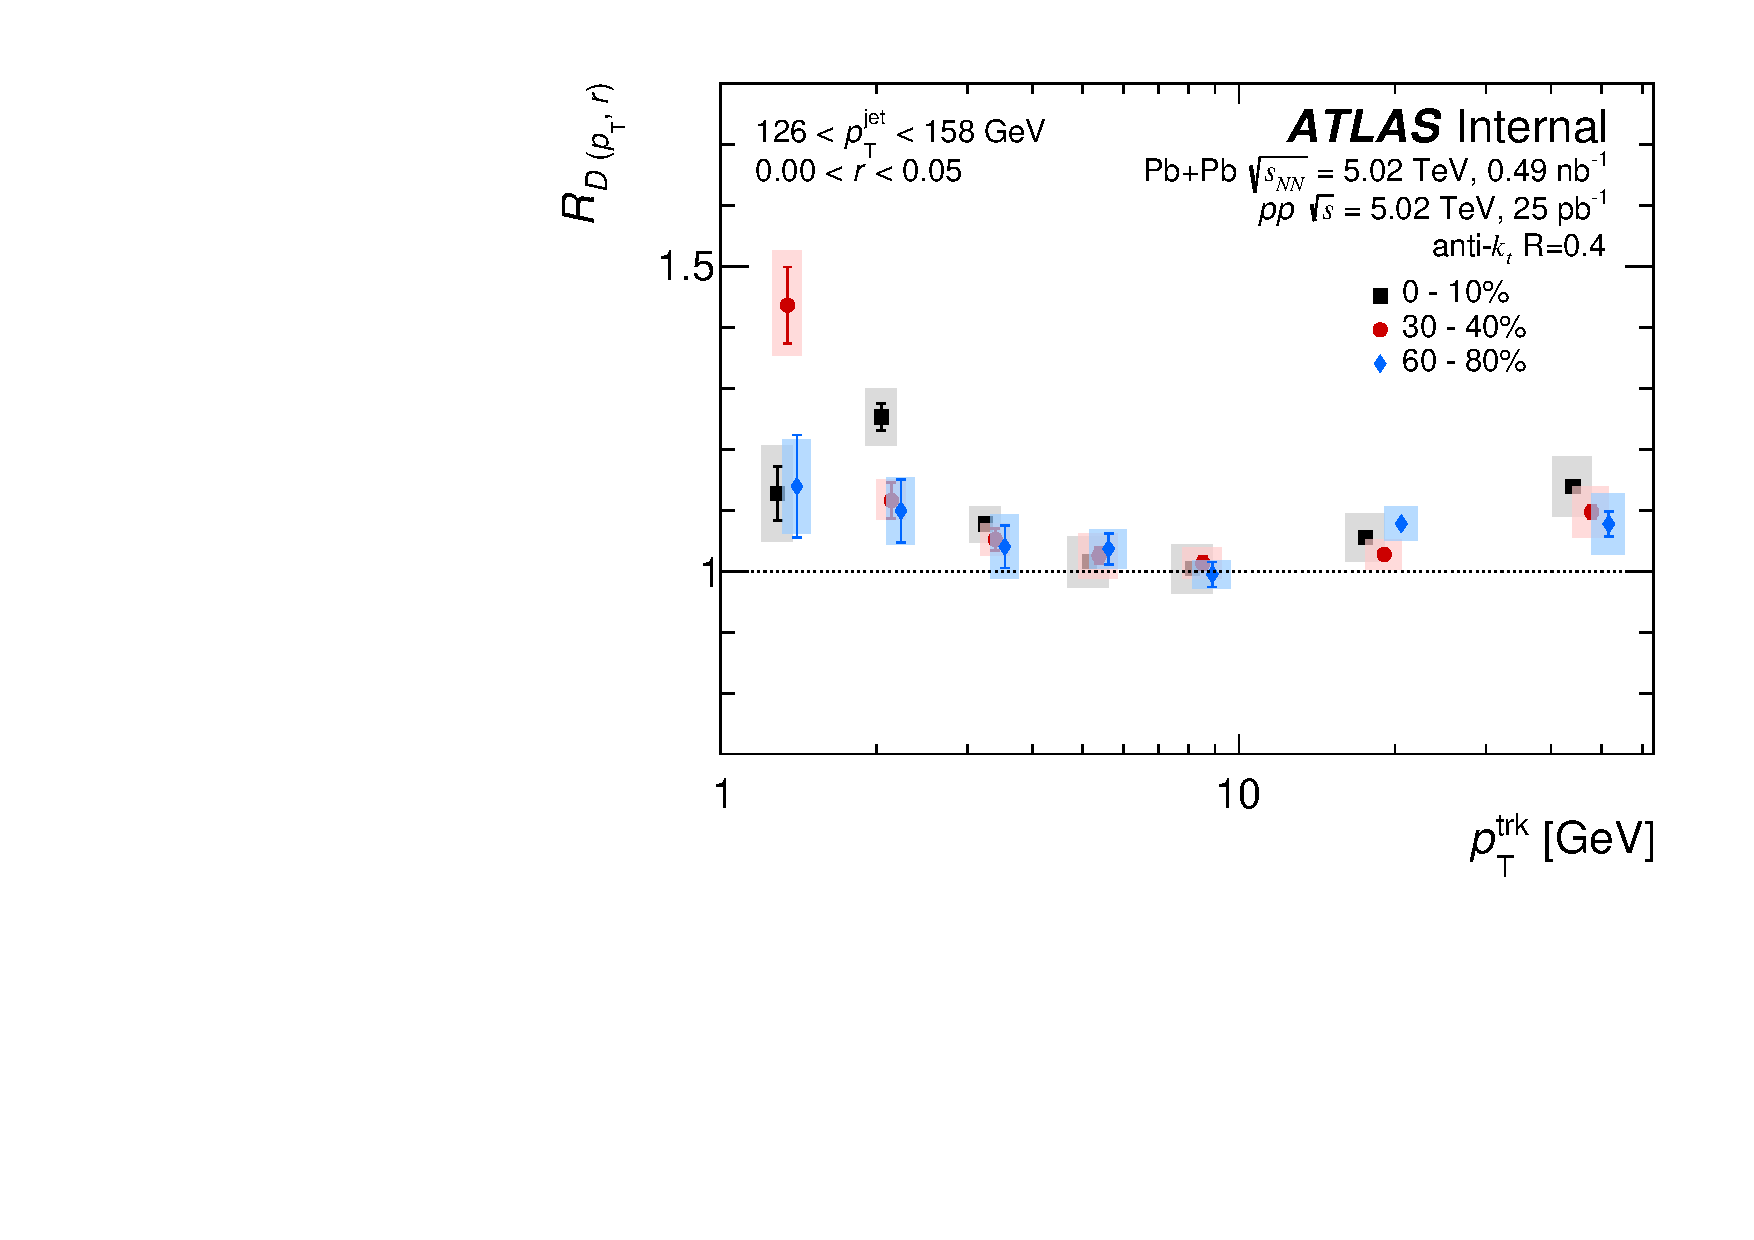
\includegraphics[width=0.5\textwidth]{results/RDpT_trkpt_jet7_dR0} &
%	 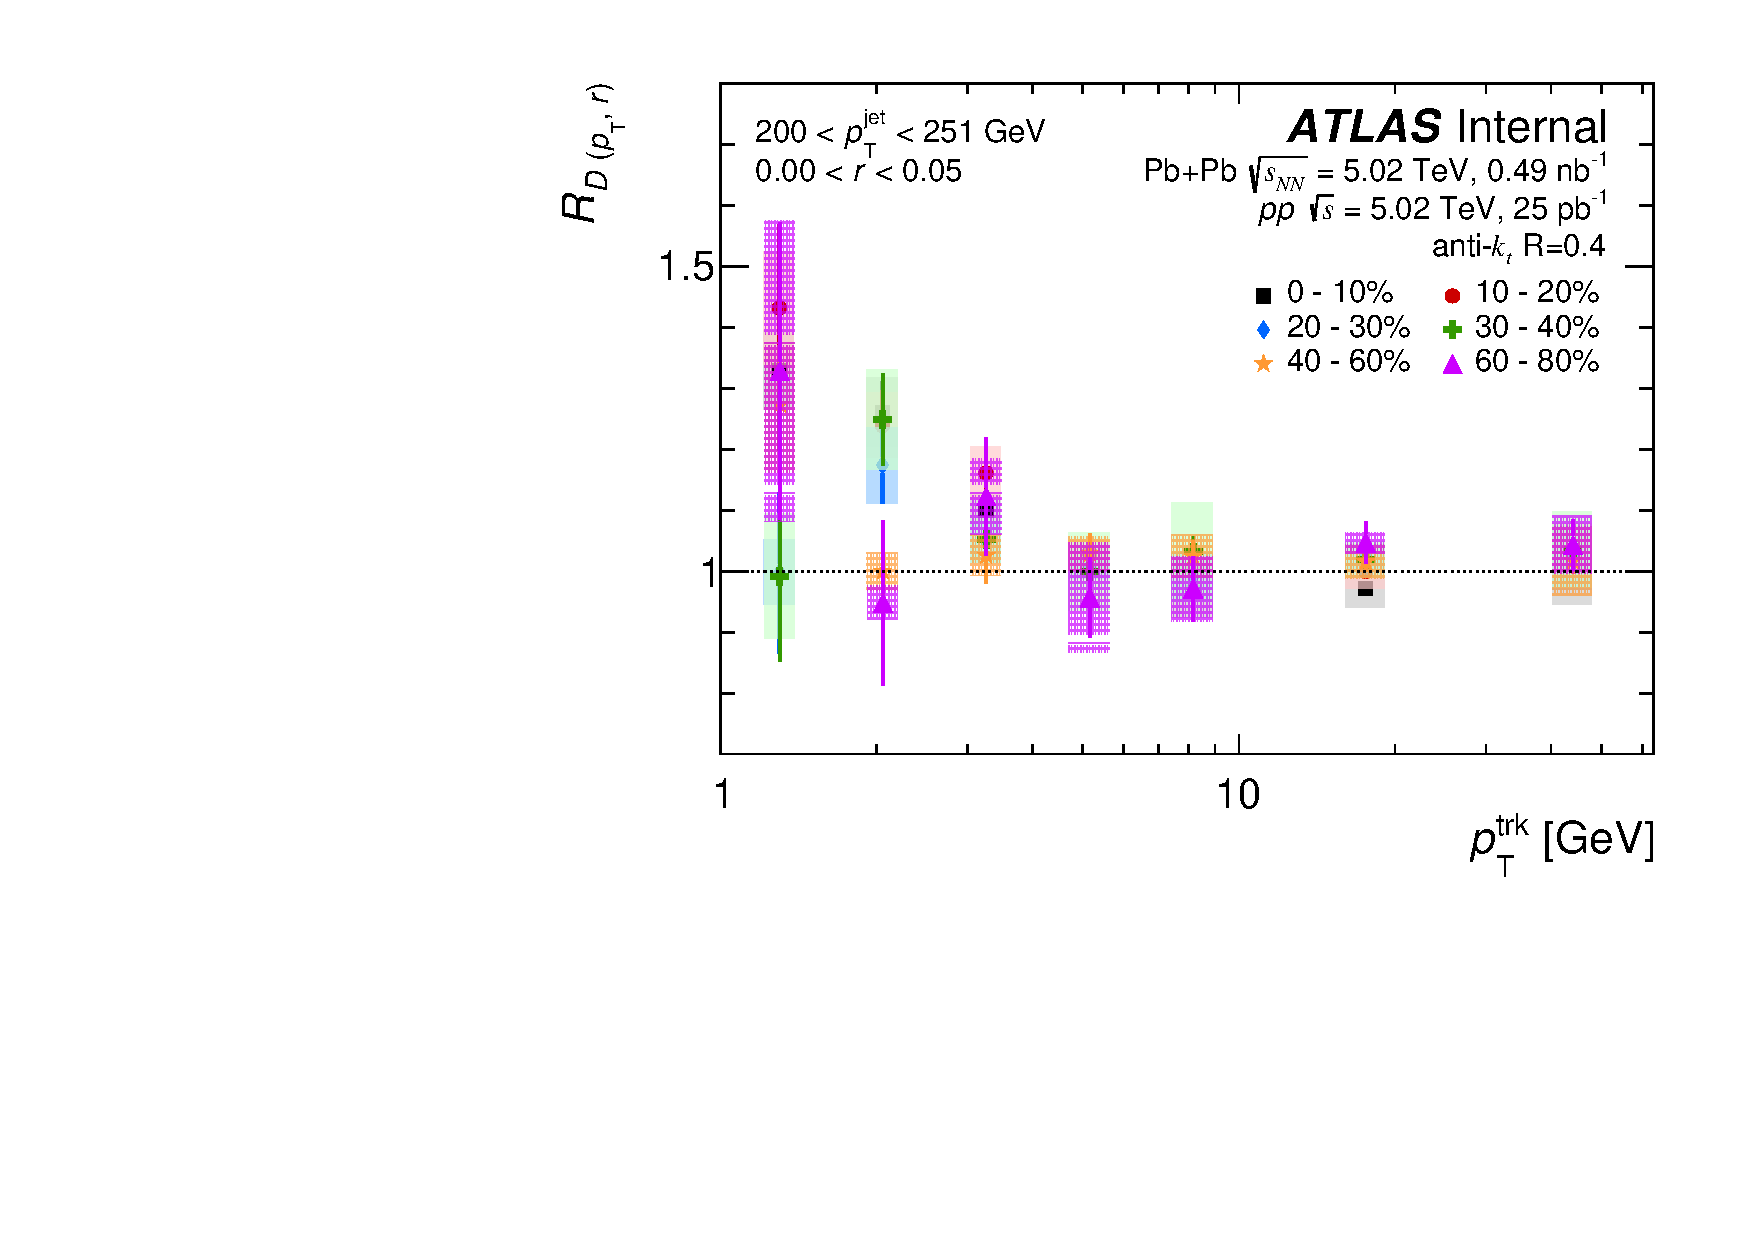
\includegraphics[width=0.5\textwidth]{results/RDpT_trkpt_jet9_dR0} \\
%	 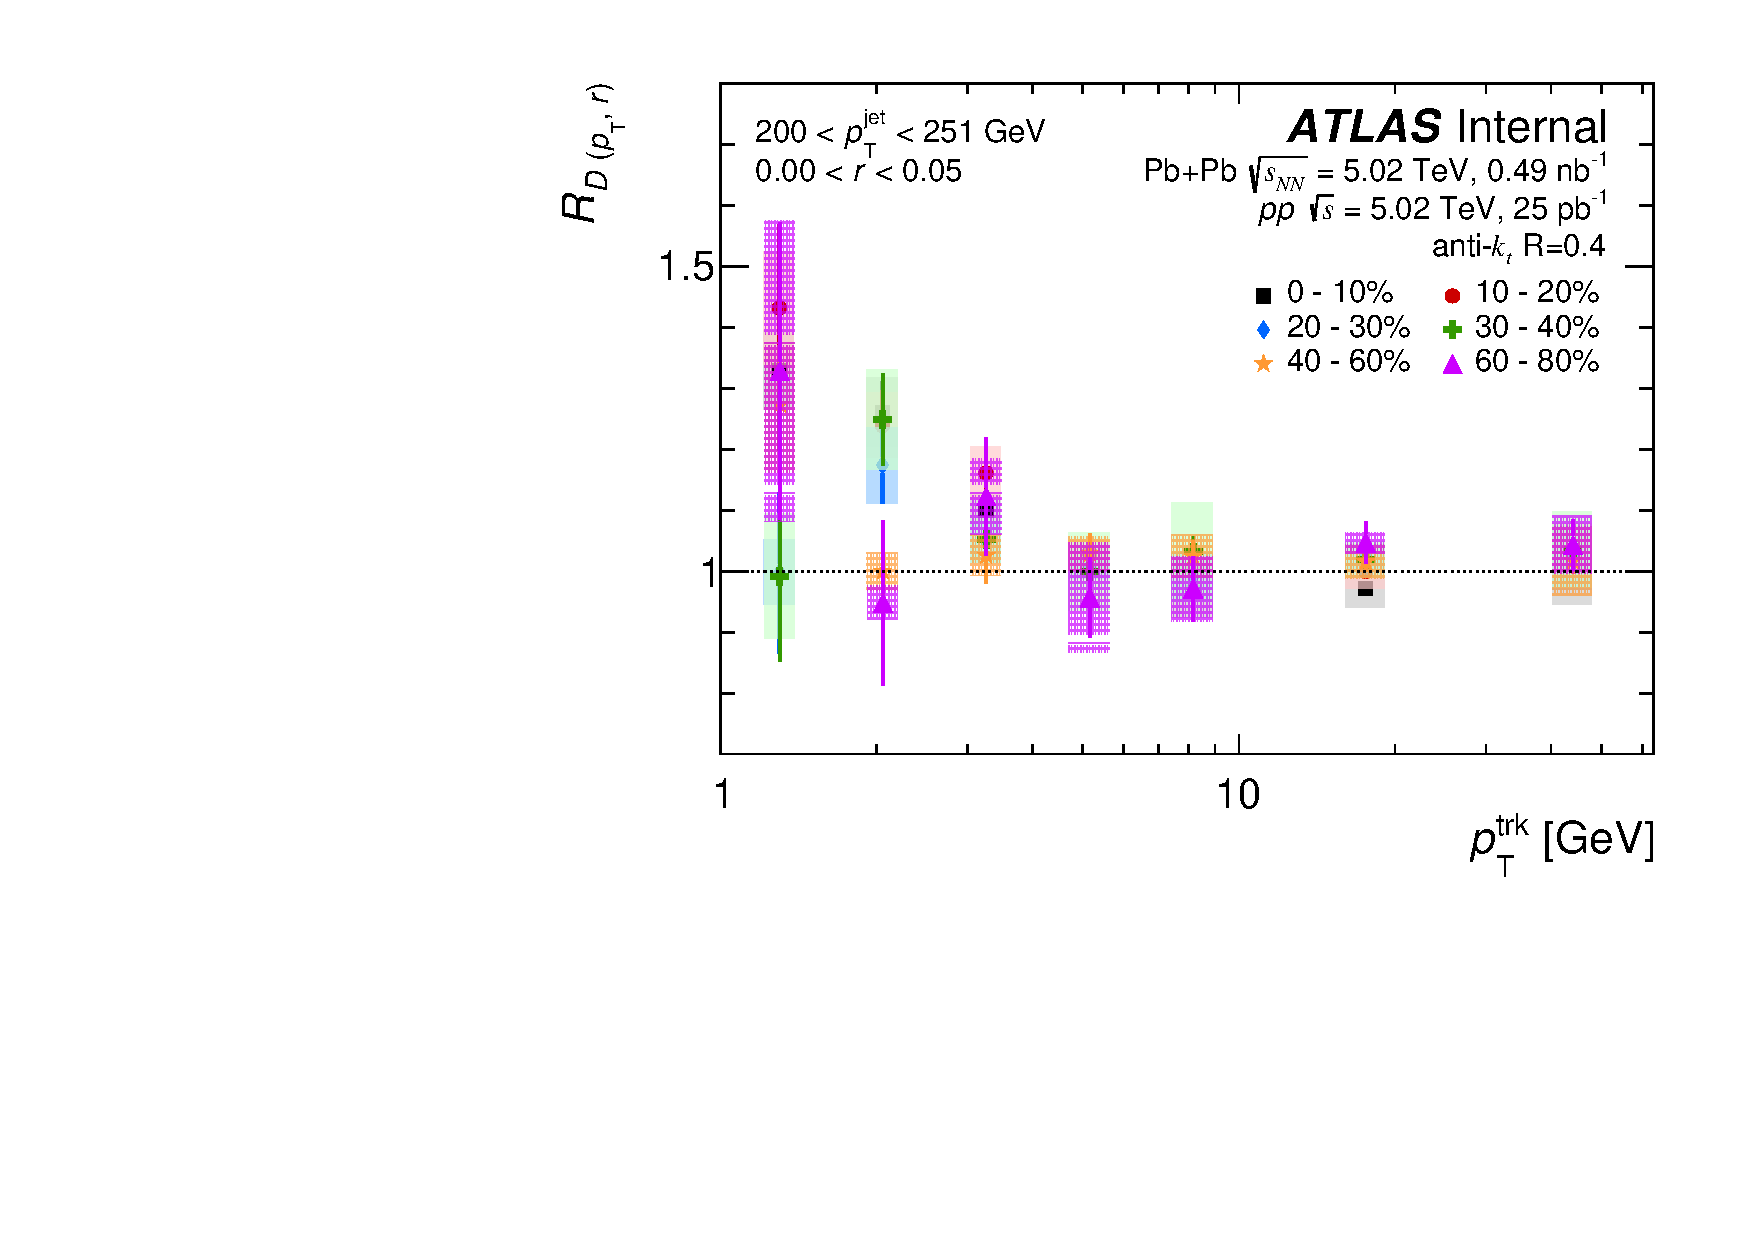
\includegraphics[width=0.5\textwidth]{results/RDpT_trkpt_jet9_dR0} &
%	 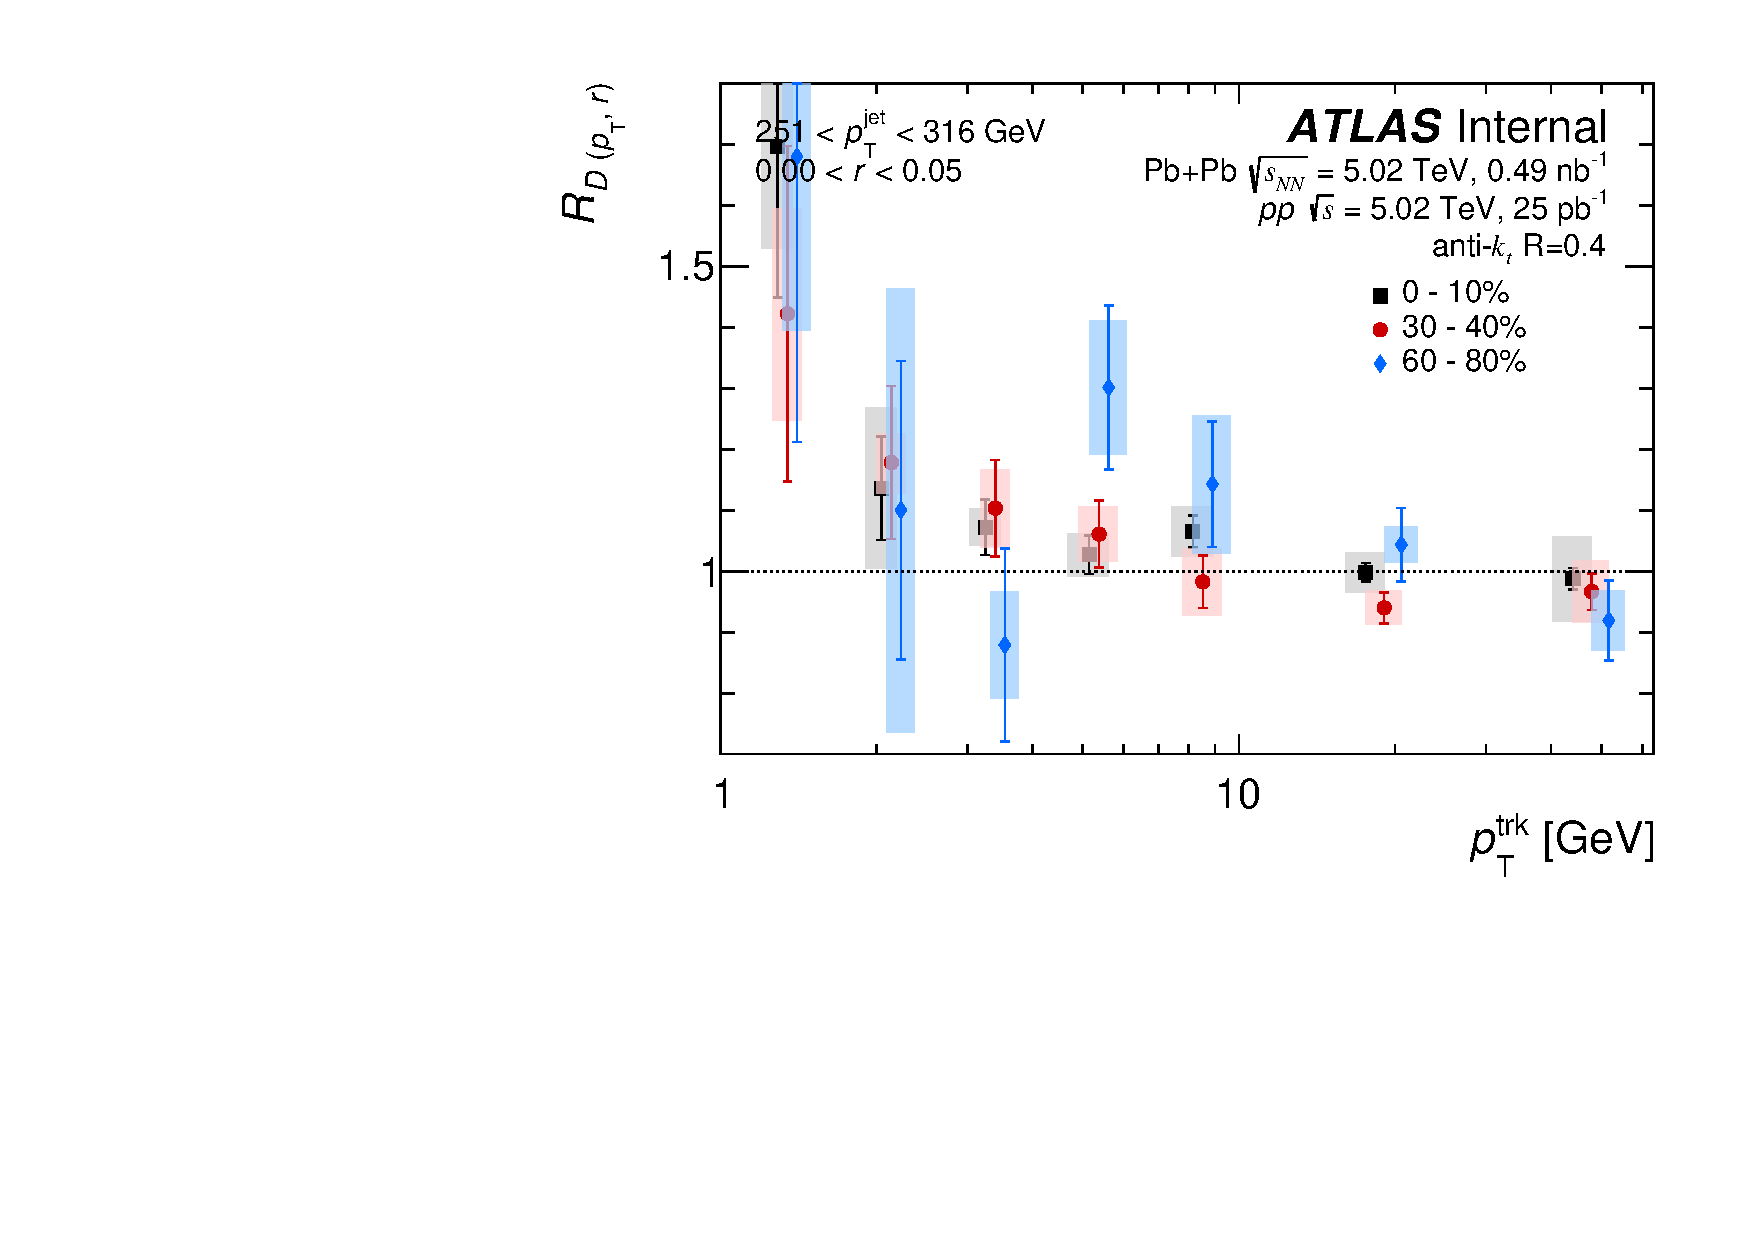
\includegraphics[width=0.5\textwidth]{results/RDpT_trkpt_jet10_dR0} \\
%	 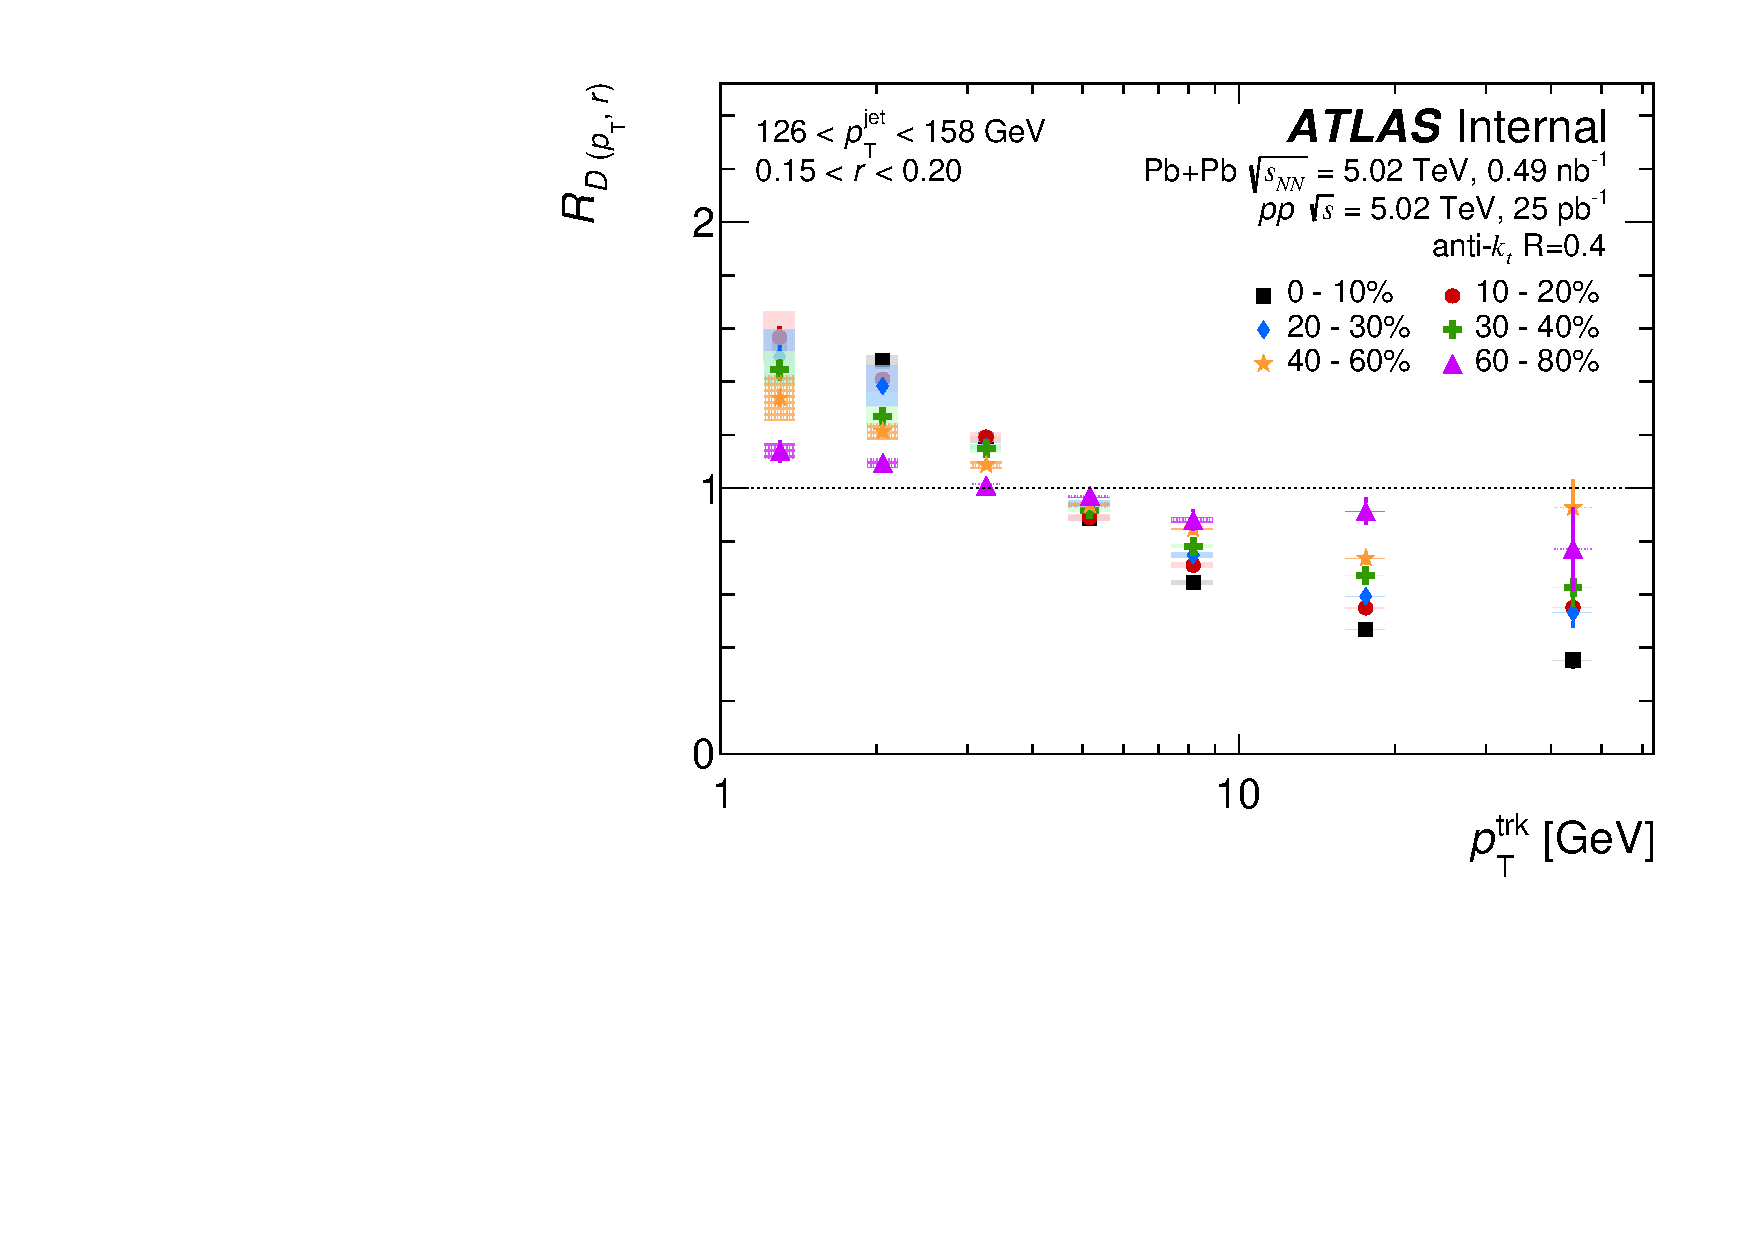
\includegraphics[width=0.5\textwidth]{results/RDpT_trkpt_jet7_dR3} &
%	 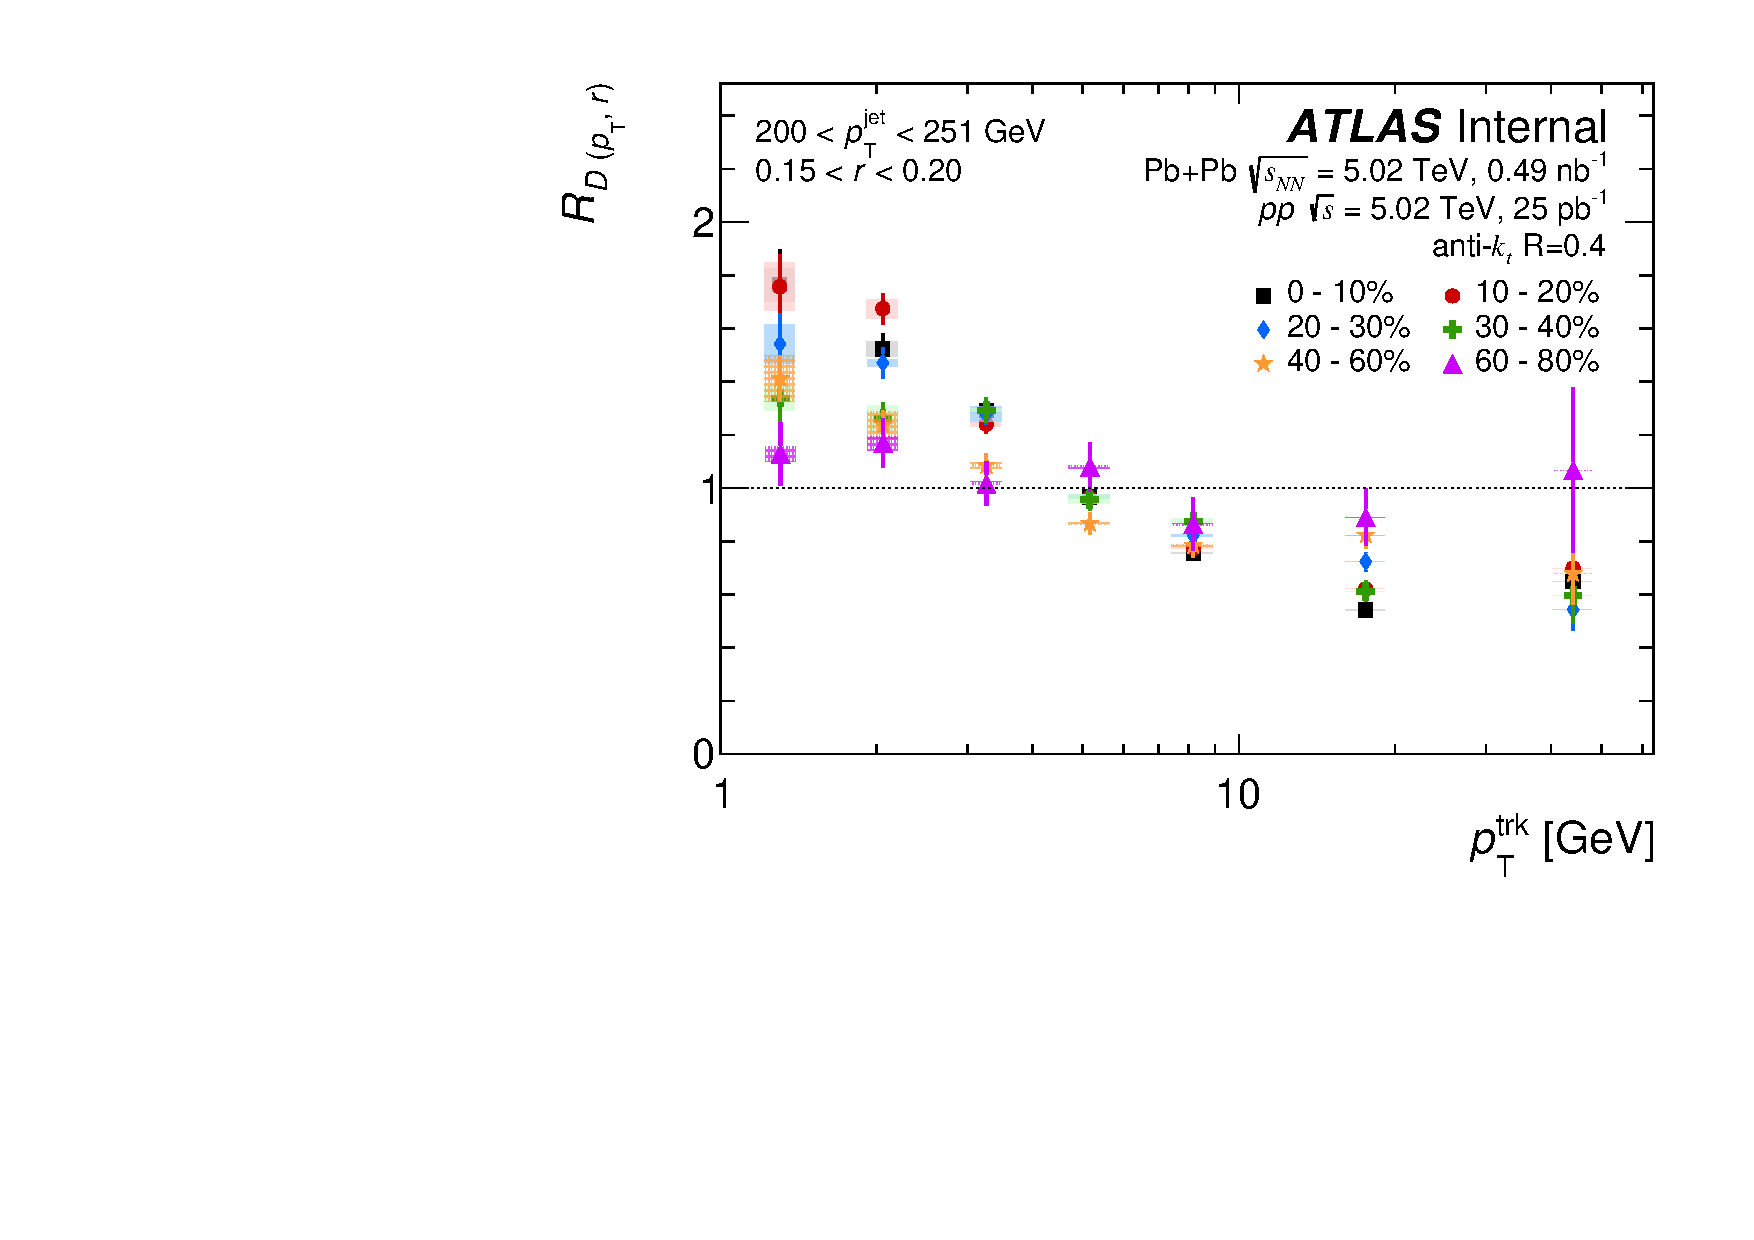
\includegraphics[width=0.5\textwidth]{results/RDpT_trkpt_jet9_dR3} \\
%	 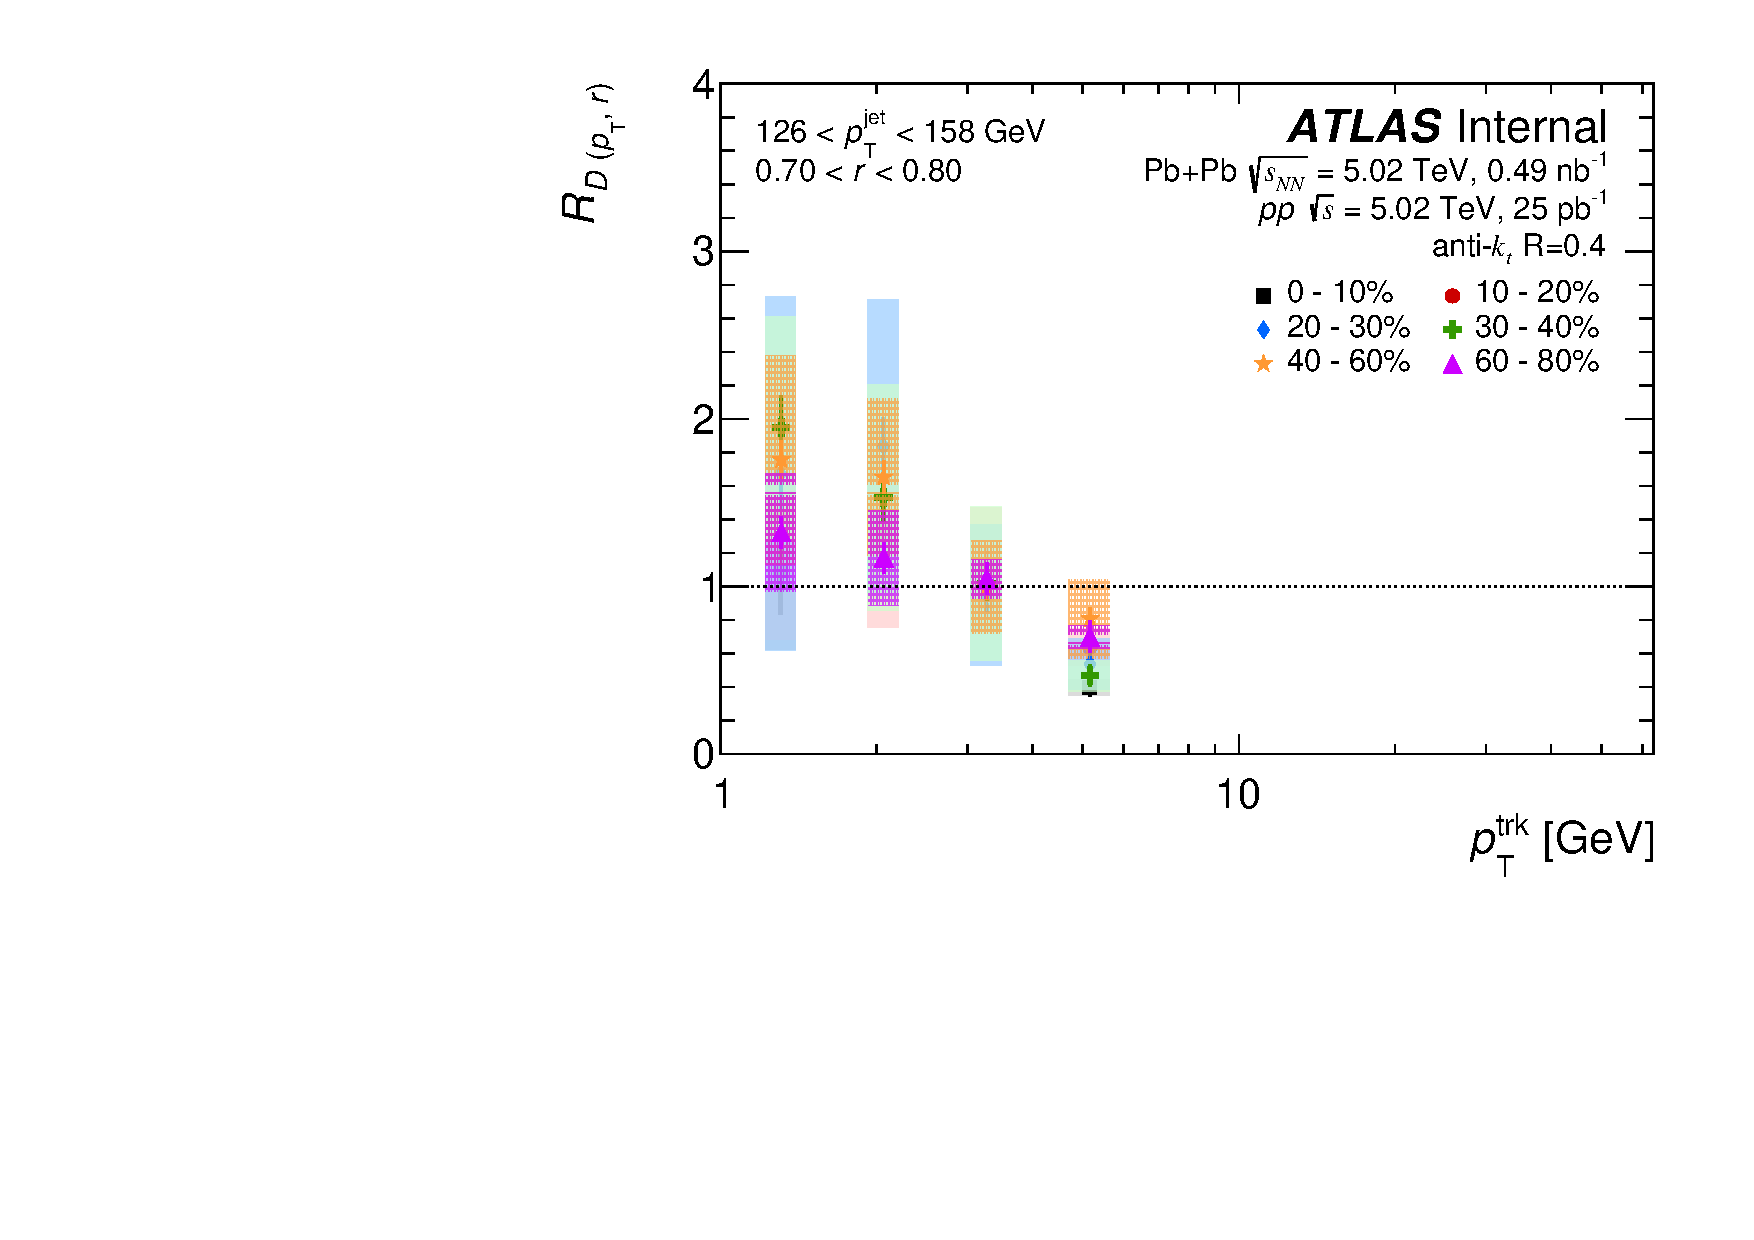
\includegraphics[width=0.5\textwidth]{results/RDpT_trkpt_jet7_dR10} &
%	 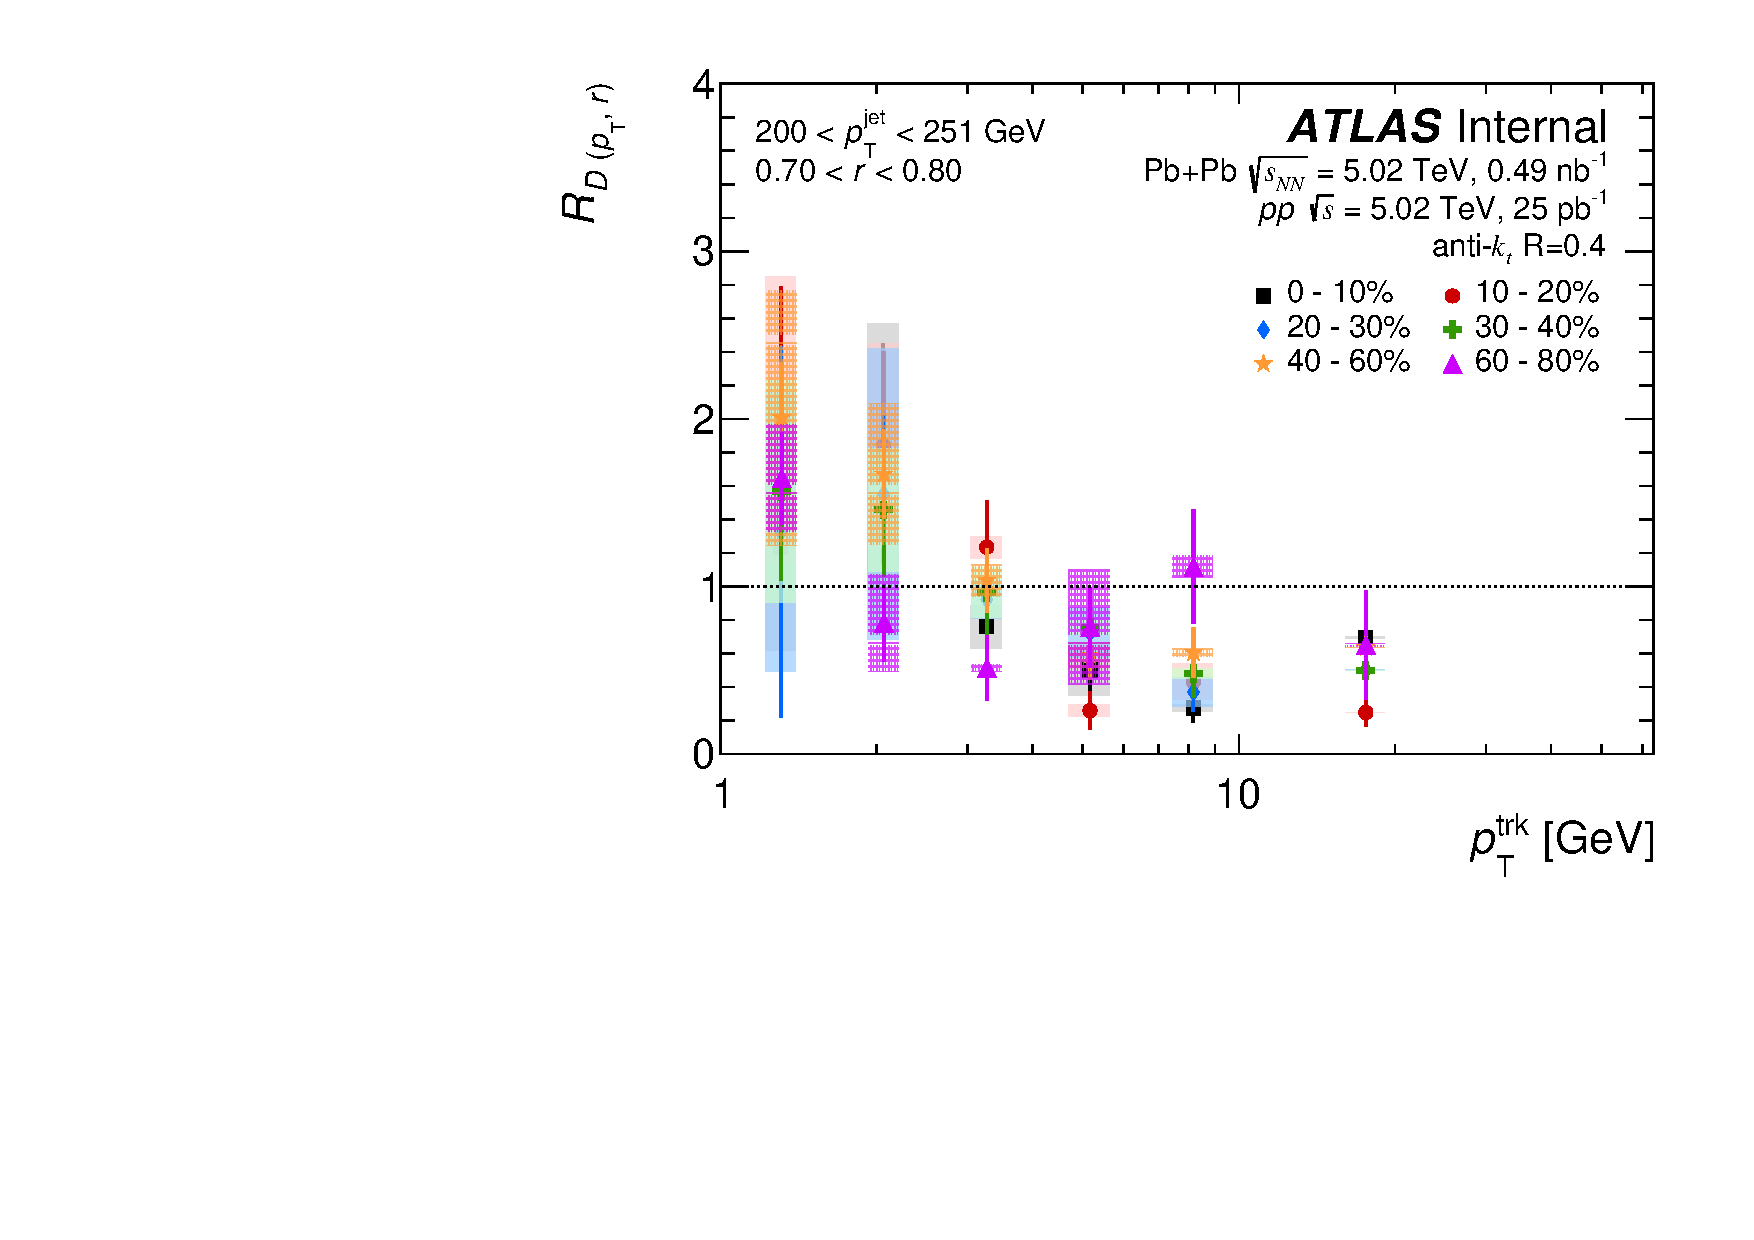
\includegraphics[width=0.5\textwidth]{results/RDpT_trkpt_jet9_dR10} \\
%\end{tabular} }
%   \caption{\RDptr\ for central \pbpb\ collisions as a function of \pt\ for different jet selections. The different colors represent different centrality bins. The vertical bars on the data points indicate statistical uncertainties while the shaded boxes indicate systematic uncertainties. The widths of the boxes are not indicative of the bin size and the points are shifted horizontally for better visibility.}
%      \label{fig:rdptr_trk_cent}
%\end{figure}
%%%%%%%%%%%%%


\FloatBarrier


\subsection{Differences of \Dptr\ distributions}
In addition to the ratios of the \Dptr\ distributions, differences between the charged particle yields are also evaluated to quantify the modification in terms of the particle density. These are given as:

\begin{align*}
\DeltaDptr = \Dptr_{\mathrm{Pb+Pb}} - \Dptr_{pp}
\end{align*}

These differences are presented as a function of $r$ for different \pt\ selections in 0--10\% central collisions in Figure~\ref{fig:deltadptr}. 
These distributions show an excess  in the charged-particle yield density for \pbpb\ collisions compared to \pp\ collisions for charged particles with $\pt <4.0$ GeV. This excess ranges from 0.5 to 4 particles per unit area per GeV for 1 \GeV\ charged particles in 126--158~\GeV\ jets for 0--10\% central \pbpb\ collisions and increases with increasing \ptjet. 
The largest excesses for charged particles with $\pt <$~4.0~\GeV\ is within the jet cone.  For large \rvar\ values, the
density decreases, but remains positive.
A depletion for higher \pt\ particles of approximately 0.5 particles per unit area per GeV is seen for 126--158~\GeV\ jets in 0--10\% central \pbpb\ collisions. The magnitude of this depletion increases for higher \ptjet. 
There is a minimum in the \DeltaDptr\ distributions of charged 
particles with \mbox{$ 4.0 < \pt <  25.1$}~\GeV\ at $0.05 < \rvar < 0.10$ that is seen at many \ptjet\ ranges under investigation.
The magnitudes of the excesses and deficits discussed here are dependent on the sizes of the charged-particle \pt\ selections
chosen.  In order to remove that dependence, Section~\ref{sec:discussion_int} provides similar quantities in which a
wider charged-particle \pt\ range is integrated over.
%For particles with 25.1~$< \pt <$~63.1~\GeV, the \DeltaDptr\ distribution is consistent with unity over the entire measured range of \rvar\ and \ptjet.

\begin{figure}
\centering{
\begin{tabular}{cc}
	 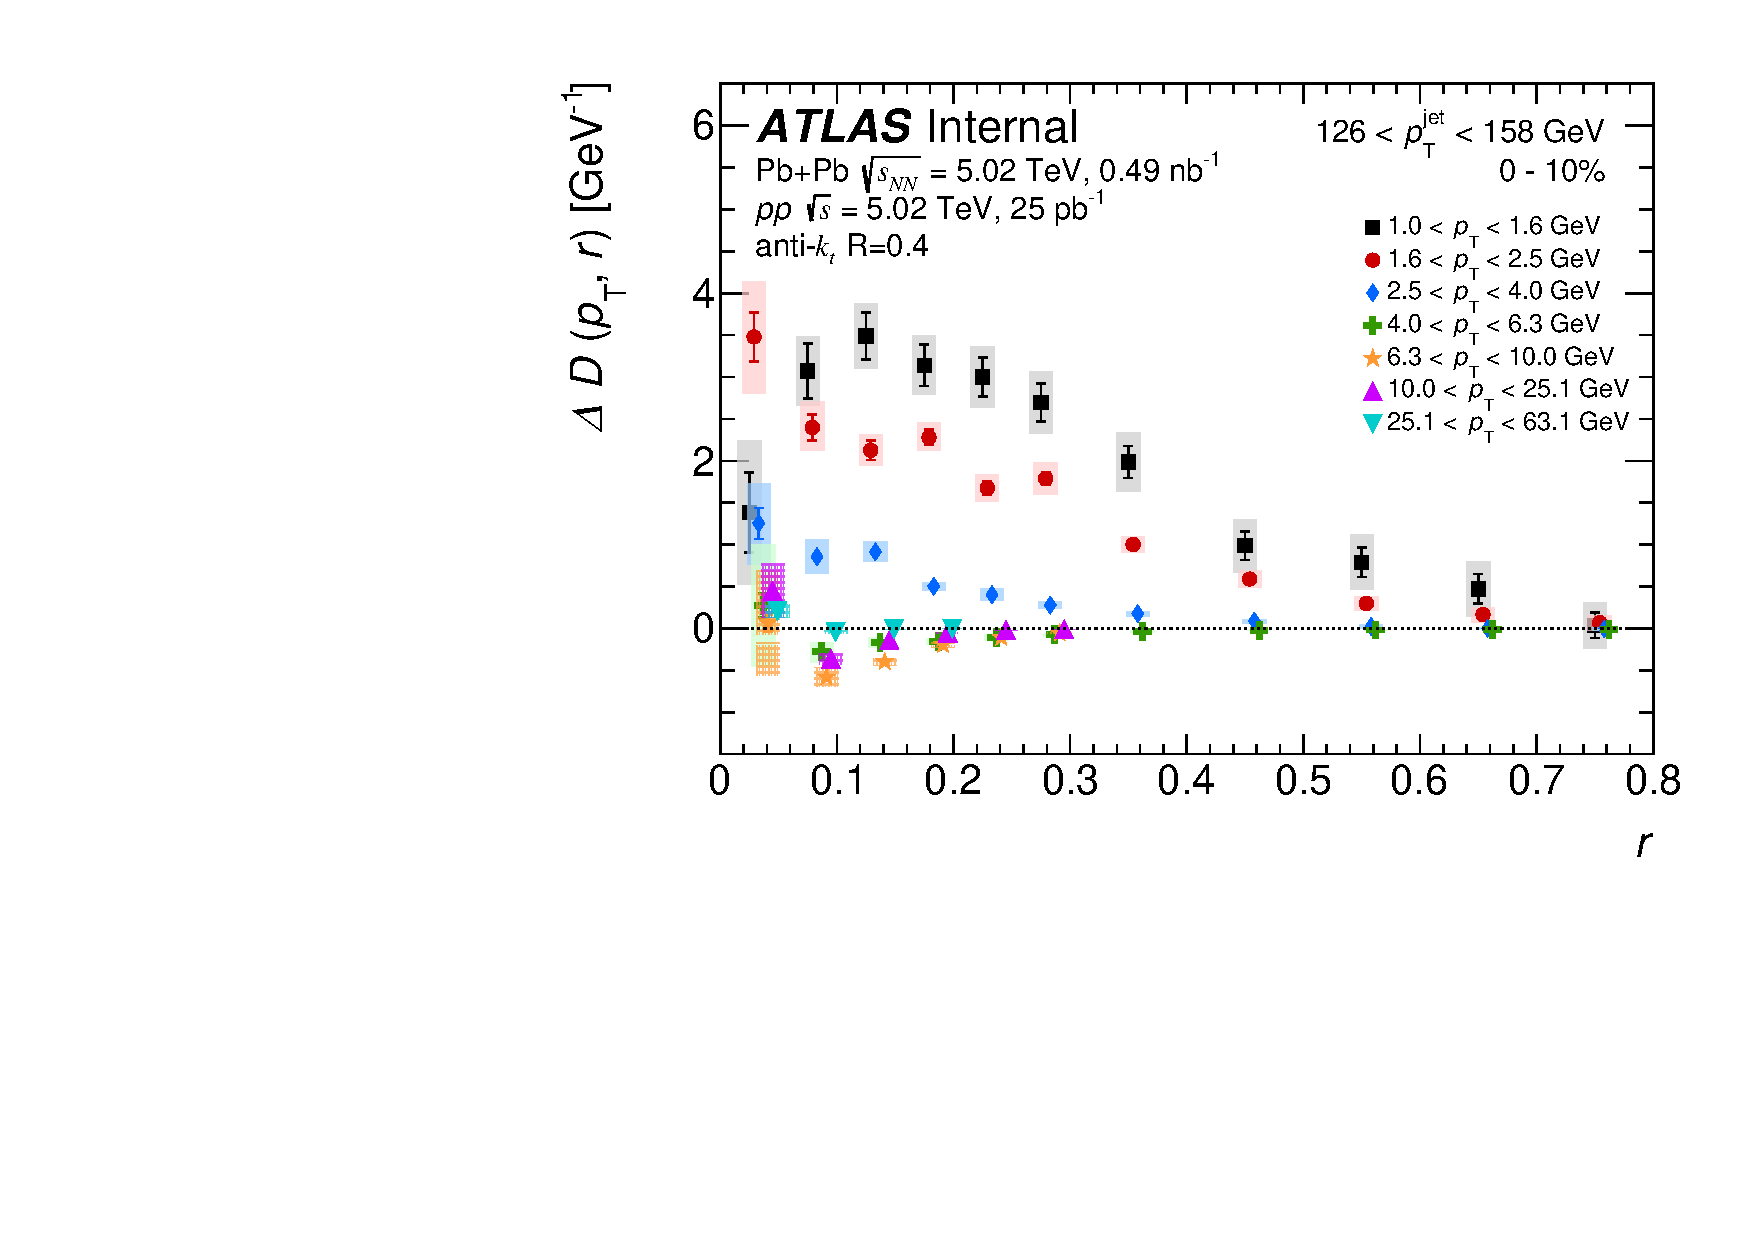
\includegraphics[width=0.5\textwidth]{results/DeltaDpT_dR_jet7_cent0} &
	 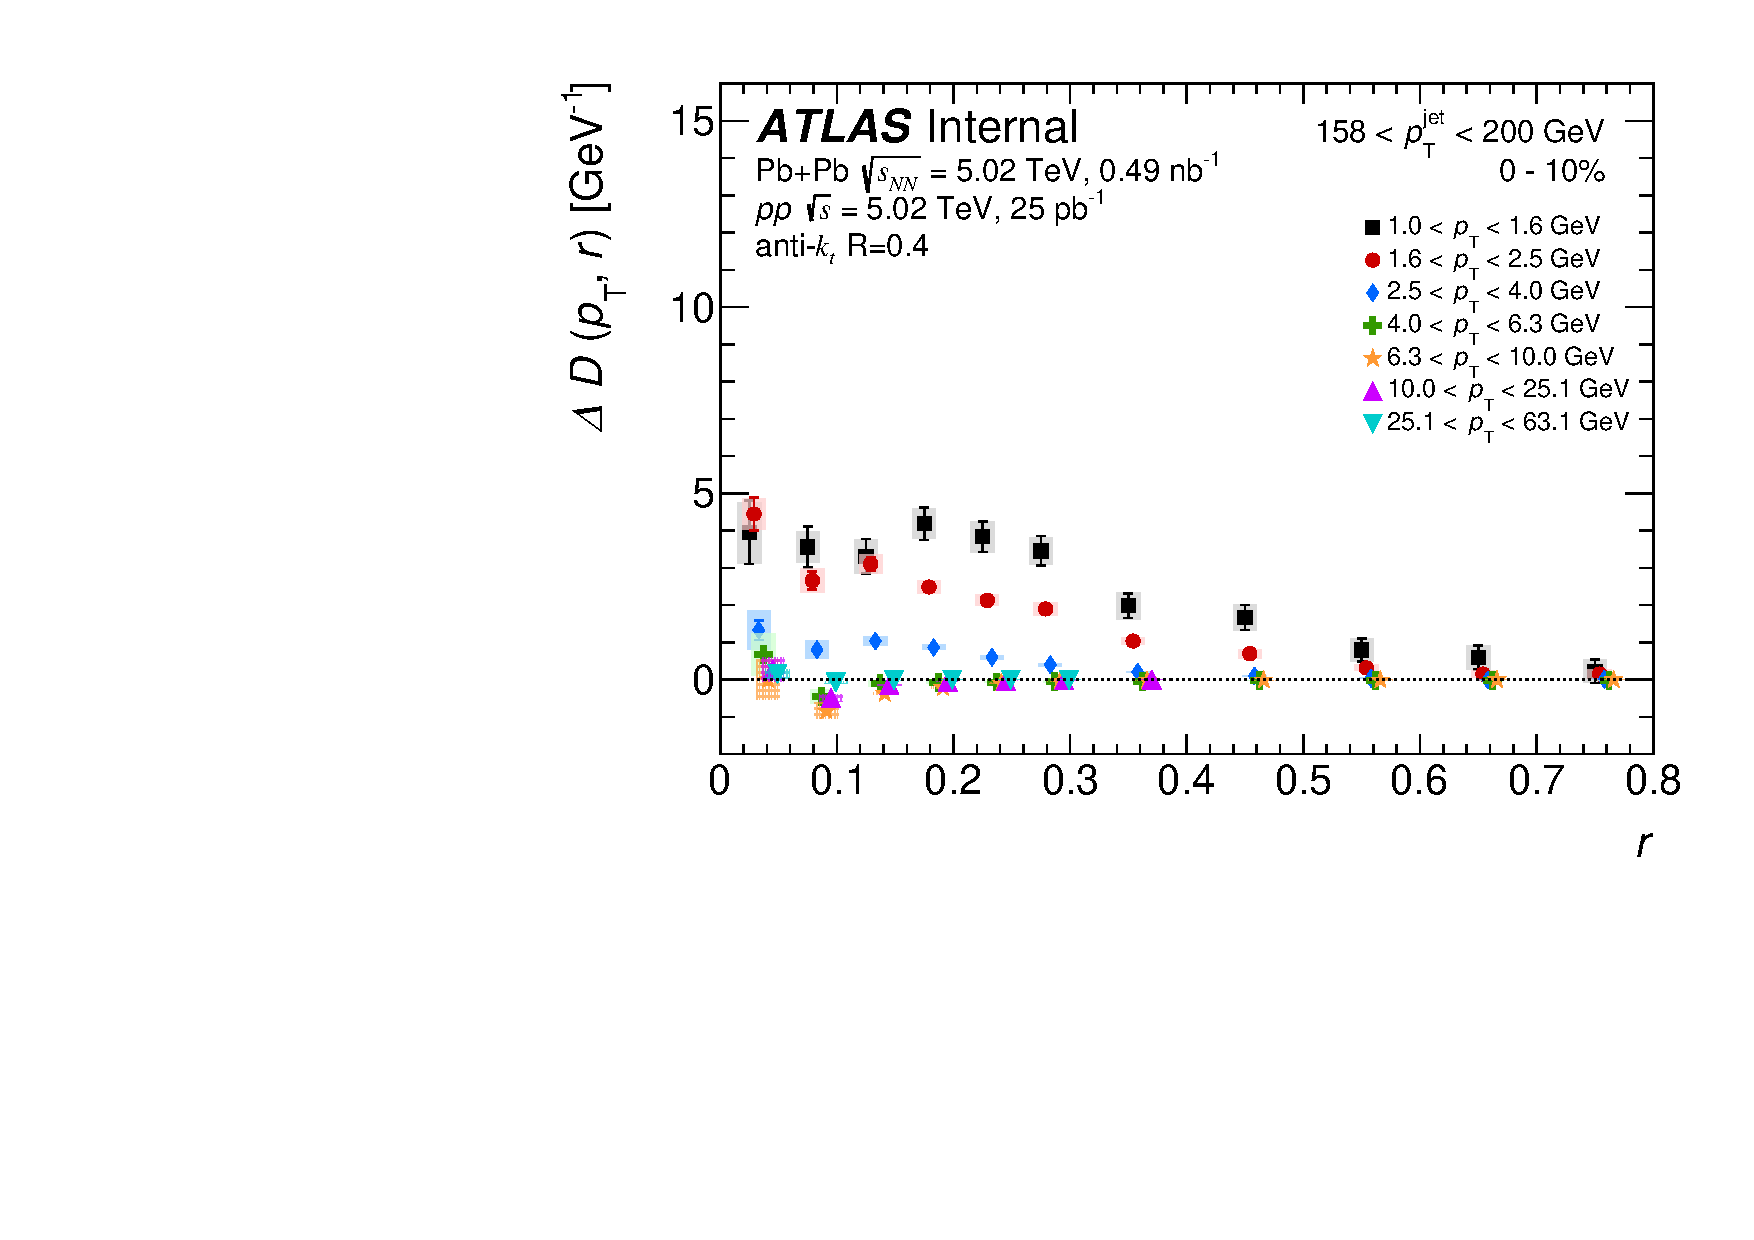
\includegraphics[width=0.5\textwidth]{results/DeltaDpT_dR_jet8_cent0} \\
	 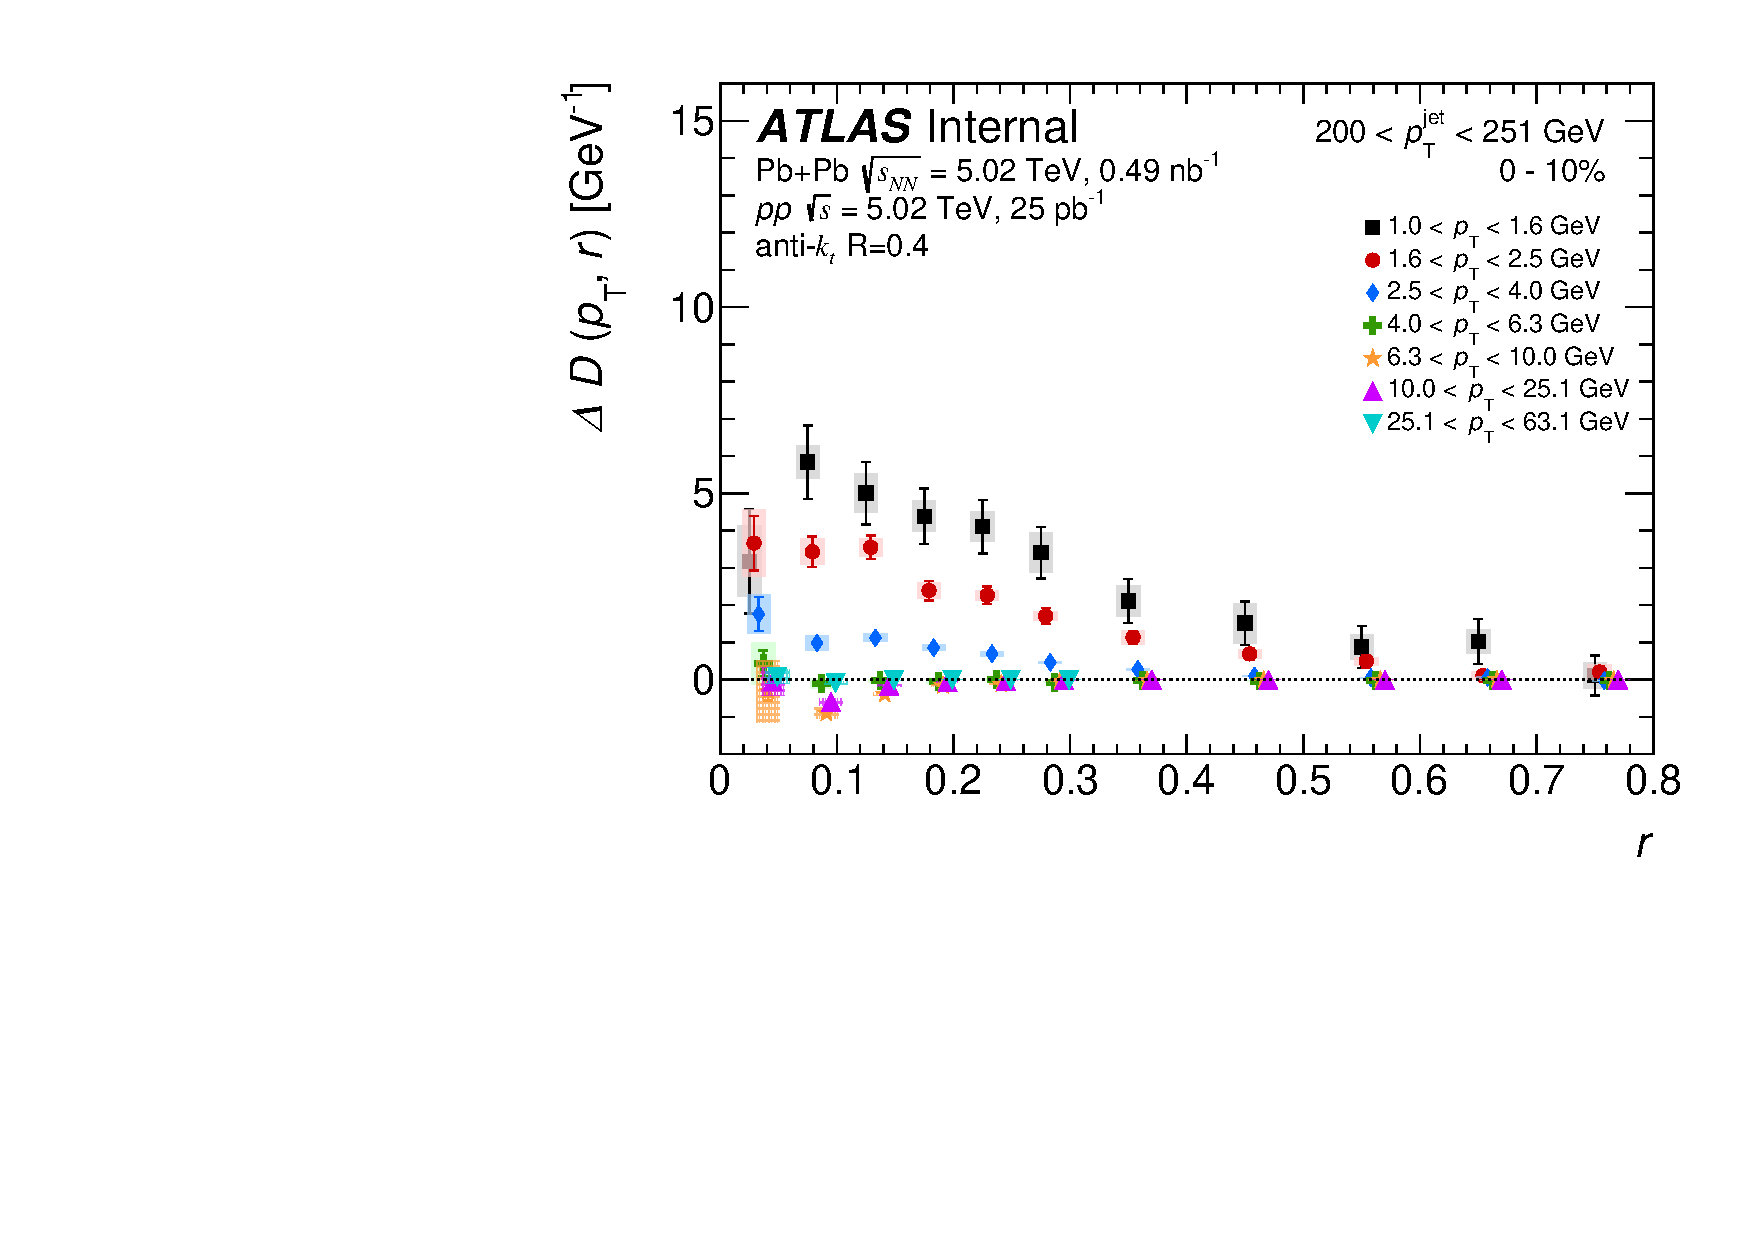
\includegraphics[width=0.5\textwidth]{results/DeltaDpT_dR_jet9_cent0} &
	 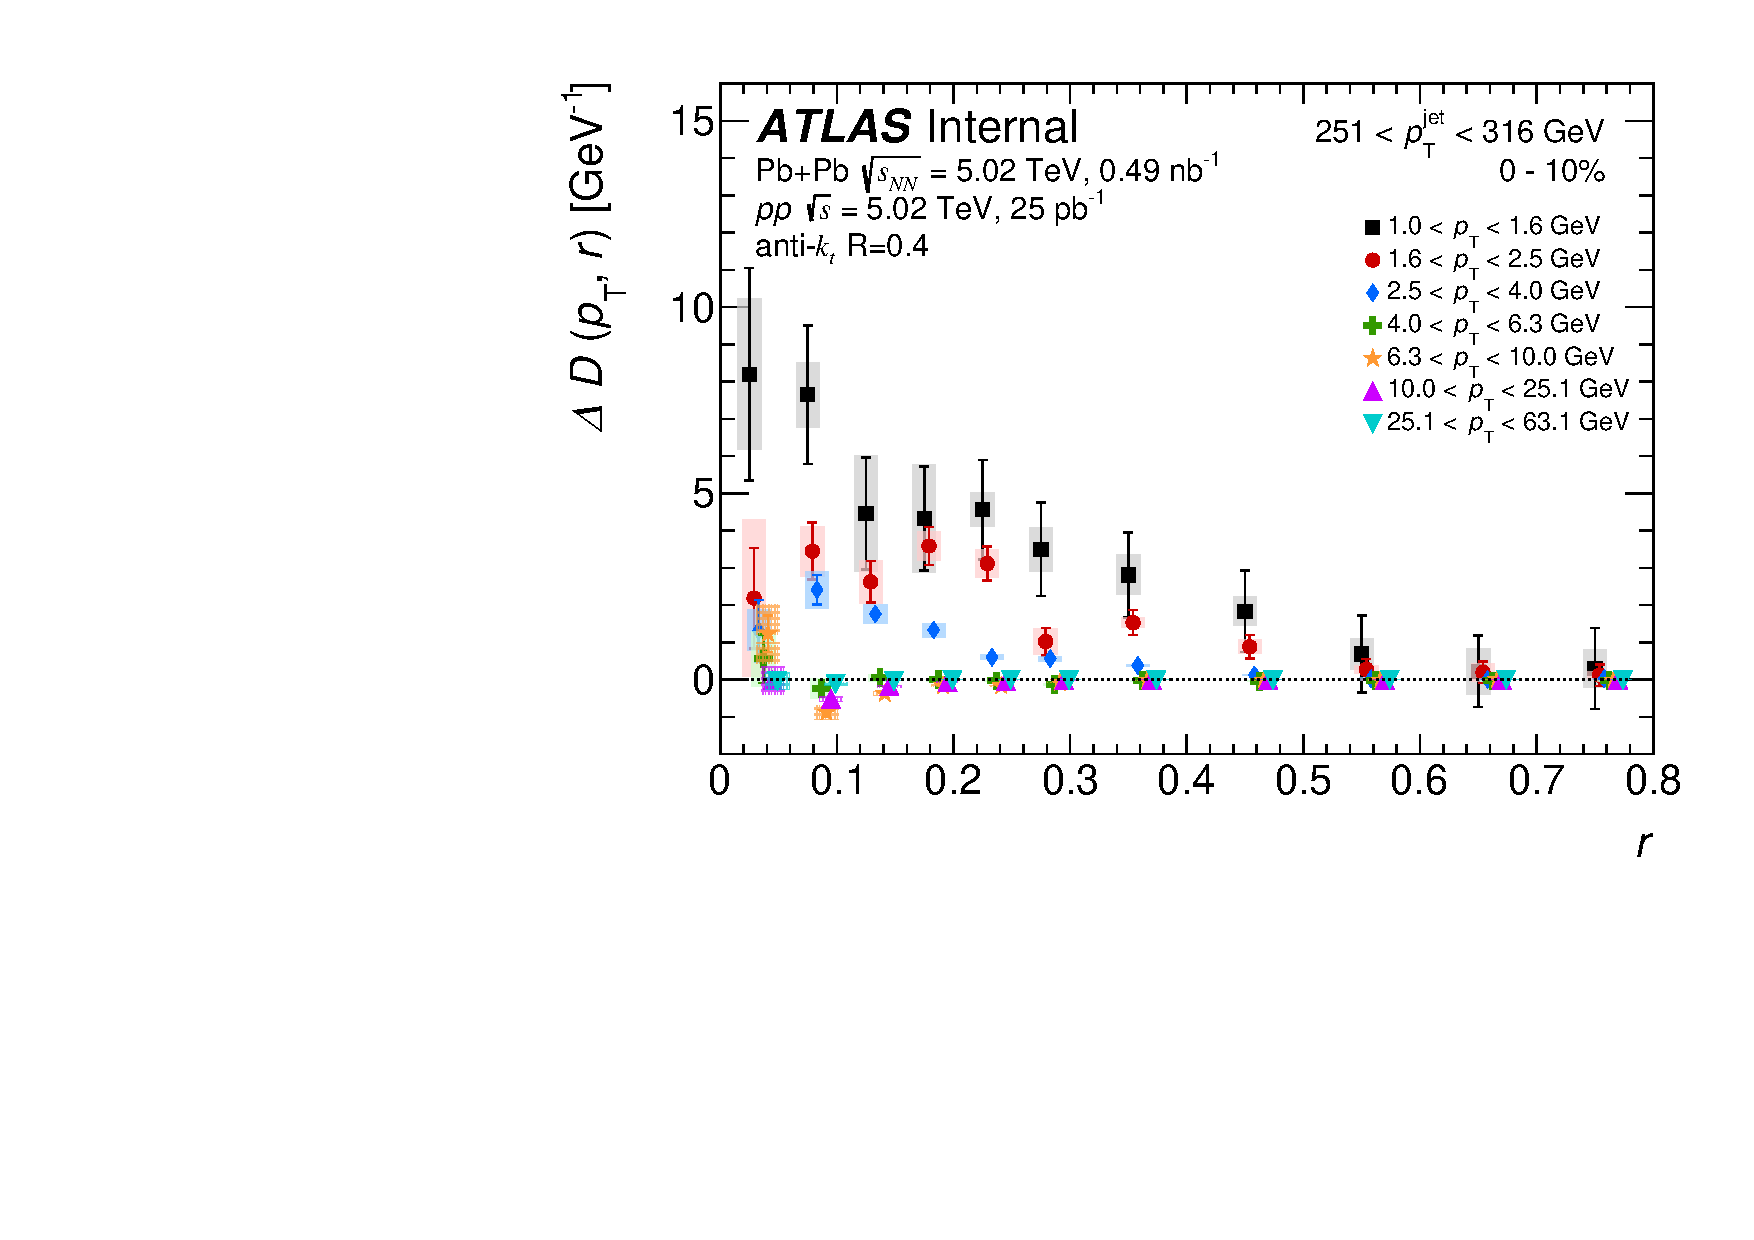
\includegraphics[width=0.5\textwidth]{results/DeltaDpT_dR_jet10_cent0} \\
\end{tabular} }
   \caption{\DeltaDptr\ as a function of \rvar\ in central collisions for all \pt\ ranges in four \ptjet\ selections: 126--158~\GeV, 158--200~\GeV, 200--251~\GeV, and 251--316~\GeV. The vertical bars on the data points indicate statistical uncertainties while the shaded boxes indicate systematic uncertainties. The widths of the boxes are not indicative of the bin size and the points are shifted horizontally for better visibility. }
      \label{fig:deltadptr}
\end{figure}
%%%%%%%%%%%%%
\FloatBarrier

\subsection{\pt\ integrated distributions}
\label{sec:discussion_int}
Motivated by similar studies of the enhancement of soft fragments in 
jet fragmentation functions in \pbpb\ compared to \pp\ collisions from \cite{Aaboud:2018hpb}, the \Dptr\ distributions can be integrated for charged particles with \pt\ < 4 GeV to construct the quantities $\Theta(\rvar)$ and $P(\rvar)$ defined as:

\begin{align*}
   \Theta(\rvar) &= \int_1^{4} \Dptr  \fd \pt \\
   P(\rvar) &= \int_0^r \int_1^{4} D(\pt, r') \fd \pt \fd r'
\end{align*}

The $\Theta(\rvar)$ values are integrated between 1.0--4.0~\GeV\ charged particles to provide a summary look at
the \pt\ region of enhancement discussed above.  The $P(\rvar)$ values further add a running integral over \rvar\
and provide information about the jet shape.
Both of these quantities can be compared between the \pp\ and \pbpb\ systems to give the following distributions:

\begin{align*}
   \Delta_{\Theta(\rvar)} &= \Theta(\rvar)_{\mathrm{Pb+Pb}} - \Theta(\rvar)_{pp} \\
   R_{\Theta(\rvar)} &= \frac{\Theta(\rvar)_{\mathrm{Pb+Pb}}}{\Theta(\rvar)_{\mathrm{pp}}} \\
   R_{P(\rvar)} &= \frac{P(\rvar)_{\mathrm{Pb+Pb}}}{P(\rvar)_{pp}}
\end{align*}

(the quantity $\Delta_{P(\rvar)}$ can also be analogously defined, but is omitted from the present discussion).
These aggregate quantities are intended to provide some summary information about the location with respect to the 
jet axis, magnitude, and \ptjet\ dependence of the low-\pt\ charged-particle excess discussed above.
The ratio quantities are useful for comparisons to other \pbpb\ measurements; $\Delta_{\Theta(\rvar)}$ is very similar 
to $\DeltaDptr$, however it is integrated over charged-particle \pt\ from 1.0--4.0~\GeV.

Figure~\ref{fig:deltaPdeltaT} shows the \DeltaTheta\ distributions as a function of \rvar\ for 0--10\%, 30--40\%,
and 60--80\% central collisions. 
In the most central collisions, a significant \ptjet\ dependence to \DeltaTheta\ is observed; for $\rvar <$~0.4 (particles
within the jet cone) \DeltaTheta\ increases with increasing \ptjet.
The value of \DeltaTheta\ decreases in more peripheral collisions and the \ptjet\ dependence is no longer significant.

%Now, the \ptjet\ dependence to the excess in charged-particle density can be seen clearly; 
%in the most central collisions
%there is an increase in \DeltaTheta\ with increasing \ptjet, but in the mid-central and peripheral collisions this is no longer
%observed within the uncertainties.

\begin{figure}
\centering{
\begin{tabular}{ccc}
	 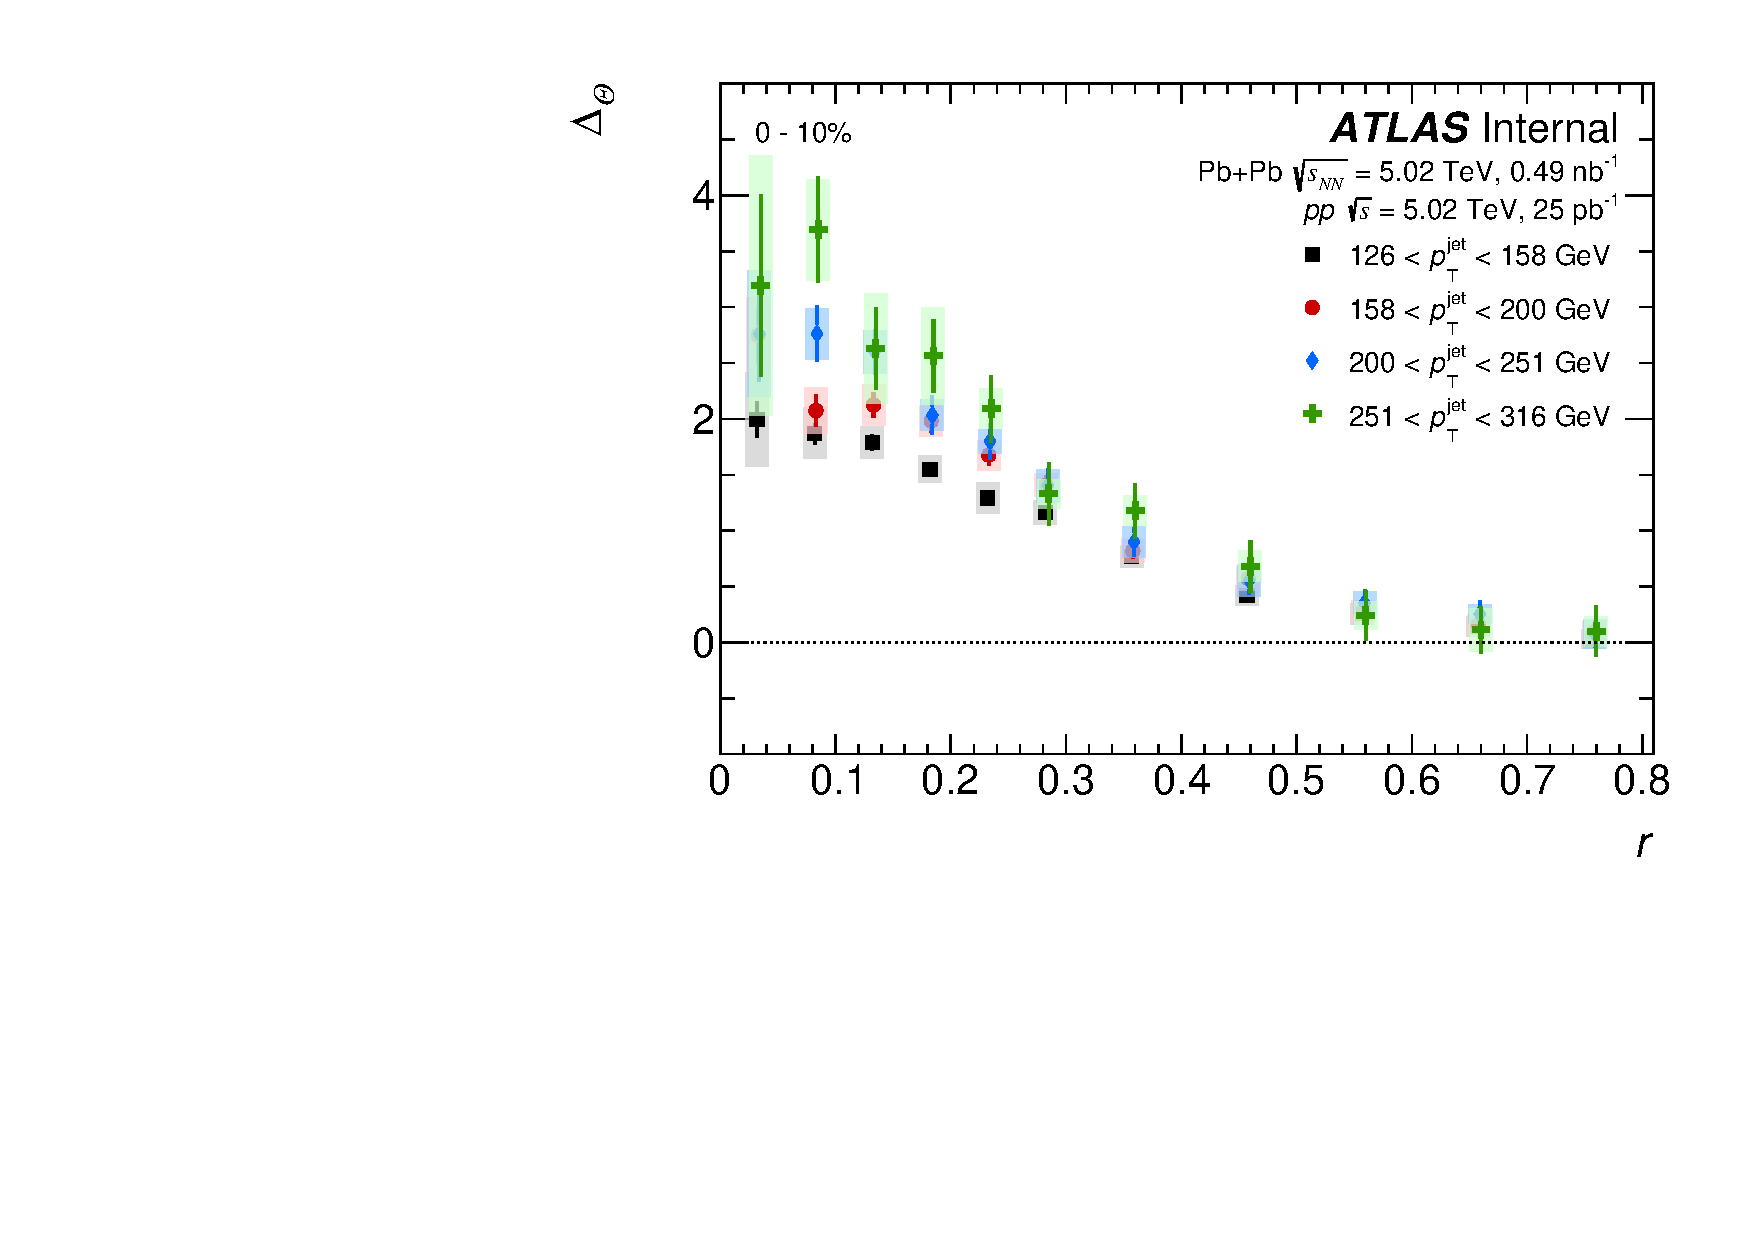
\includegraphics[width=0.48\textwidth]{results/DeltaDpT_lowpt_integ_cent0.pdf}
   %	 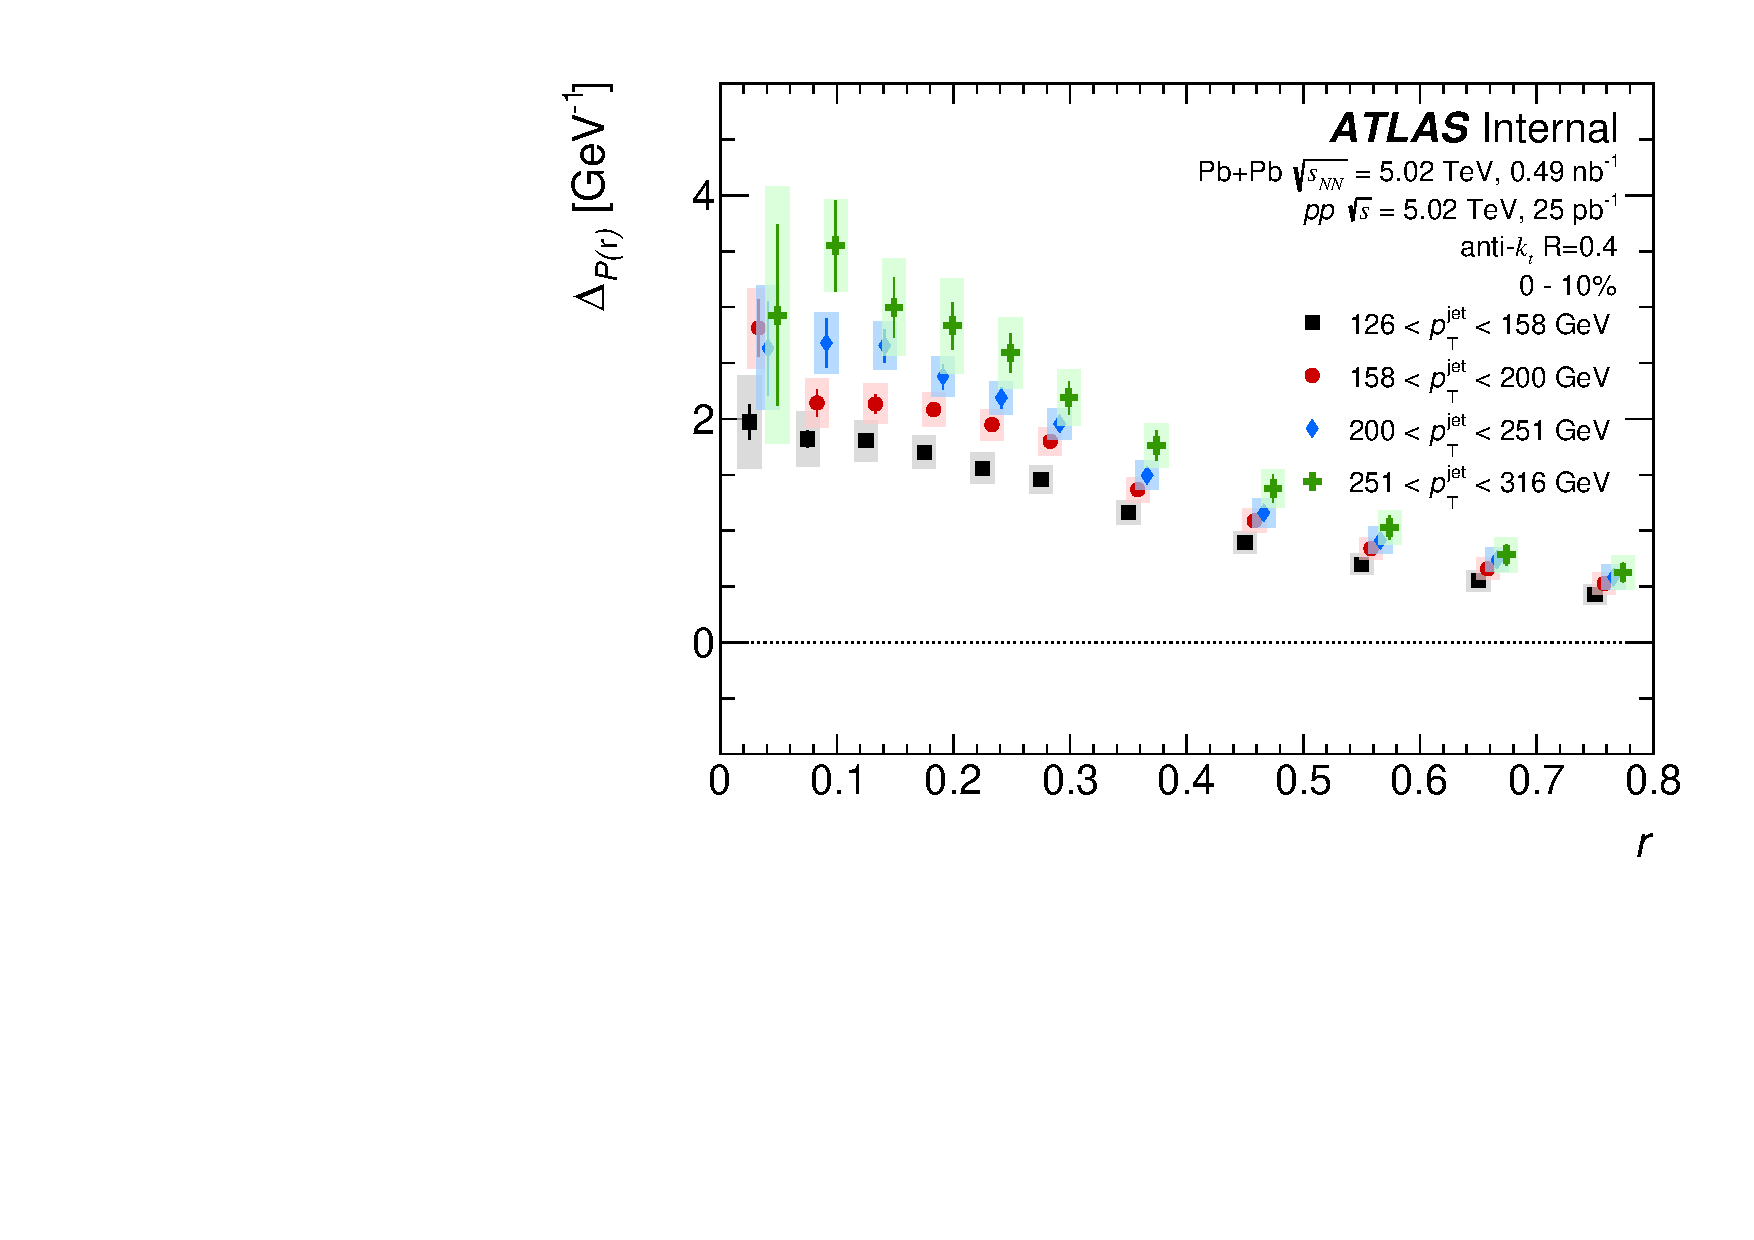
\includegraphics[width=0.5\textwidth]{results/DeltaDpT_jetshape_cent0.pdf} \\
	 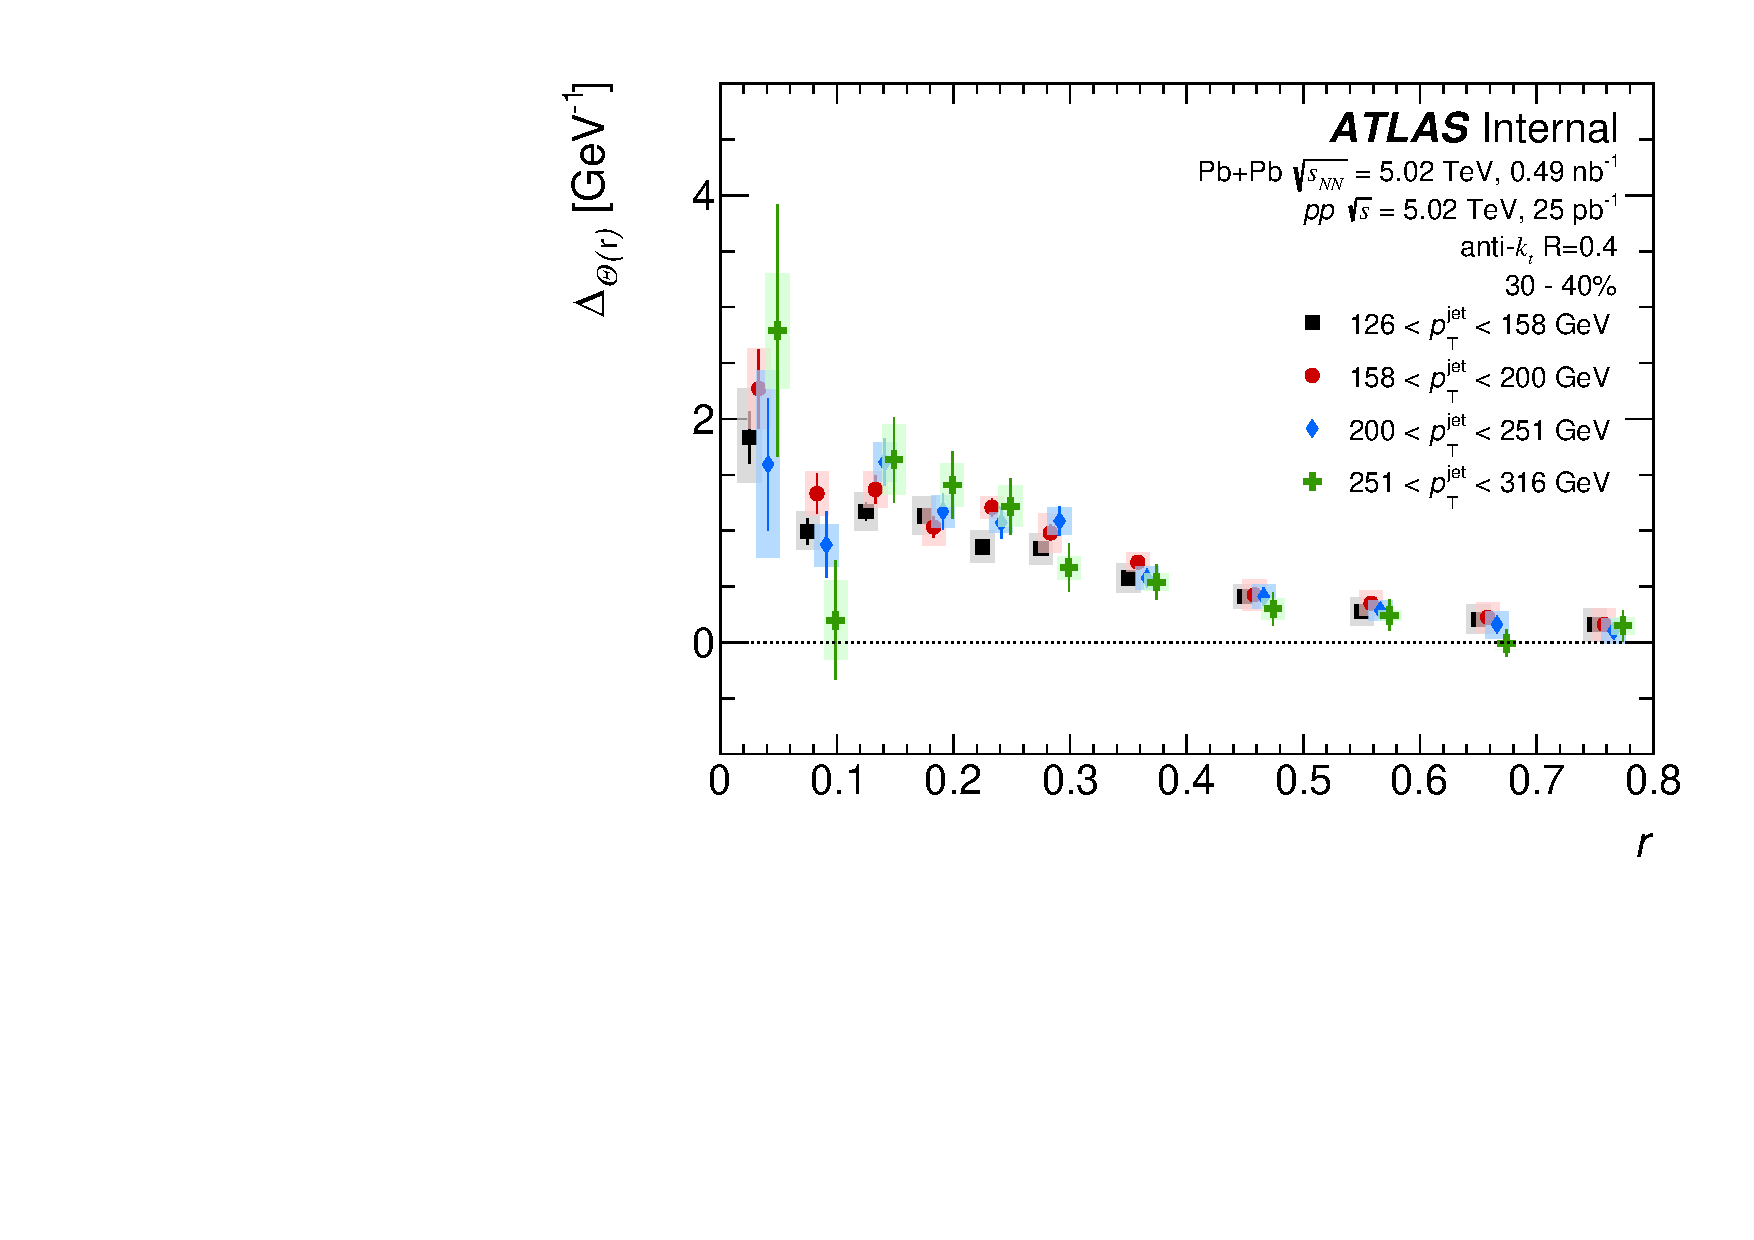
\includegraphics[width=0.48\textwidth]{results/DeltaDpT_lowpt_integ_cent3.pdf} \\
%	 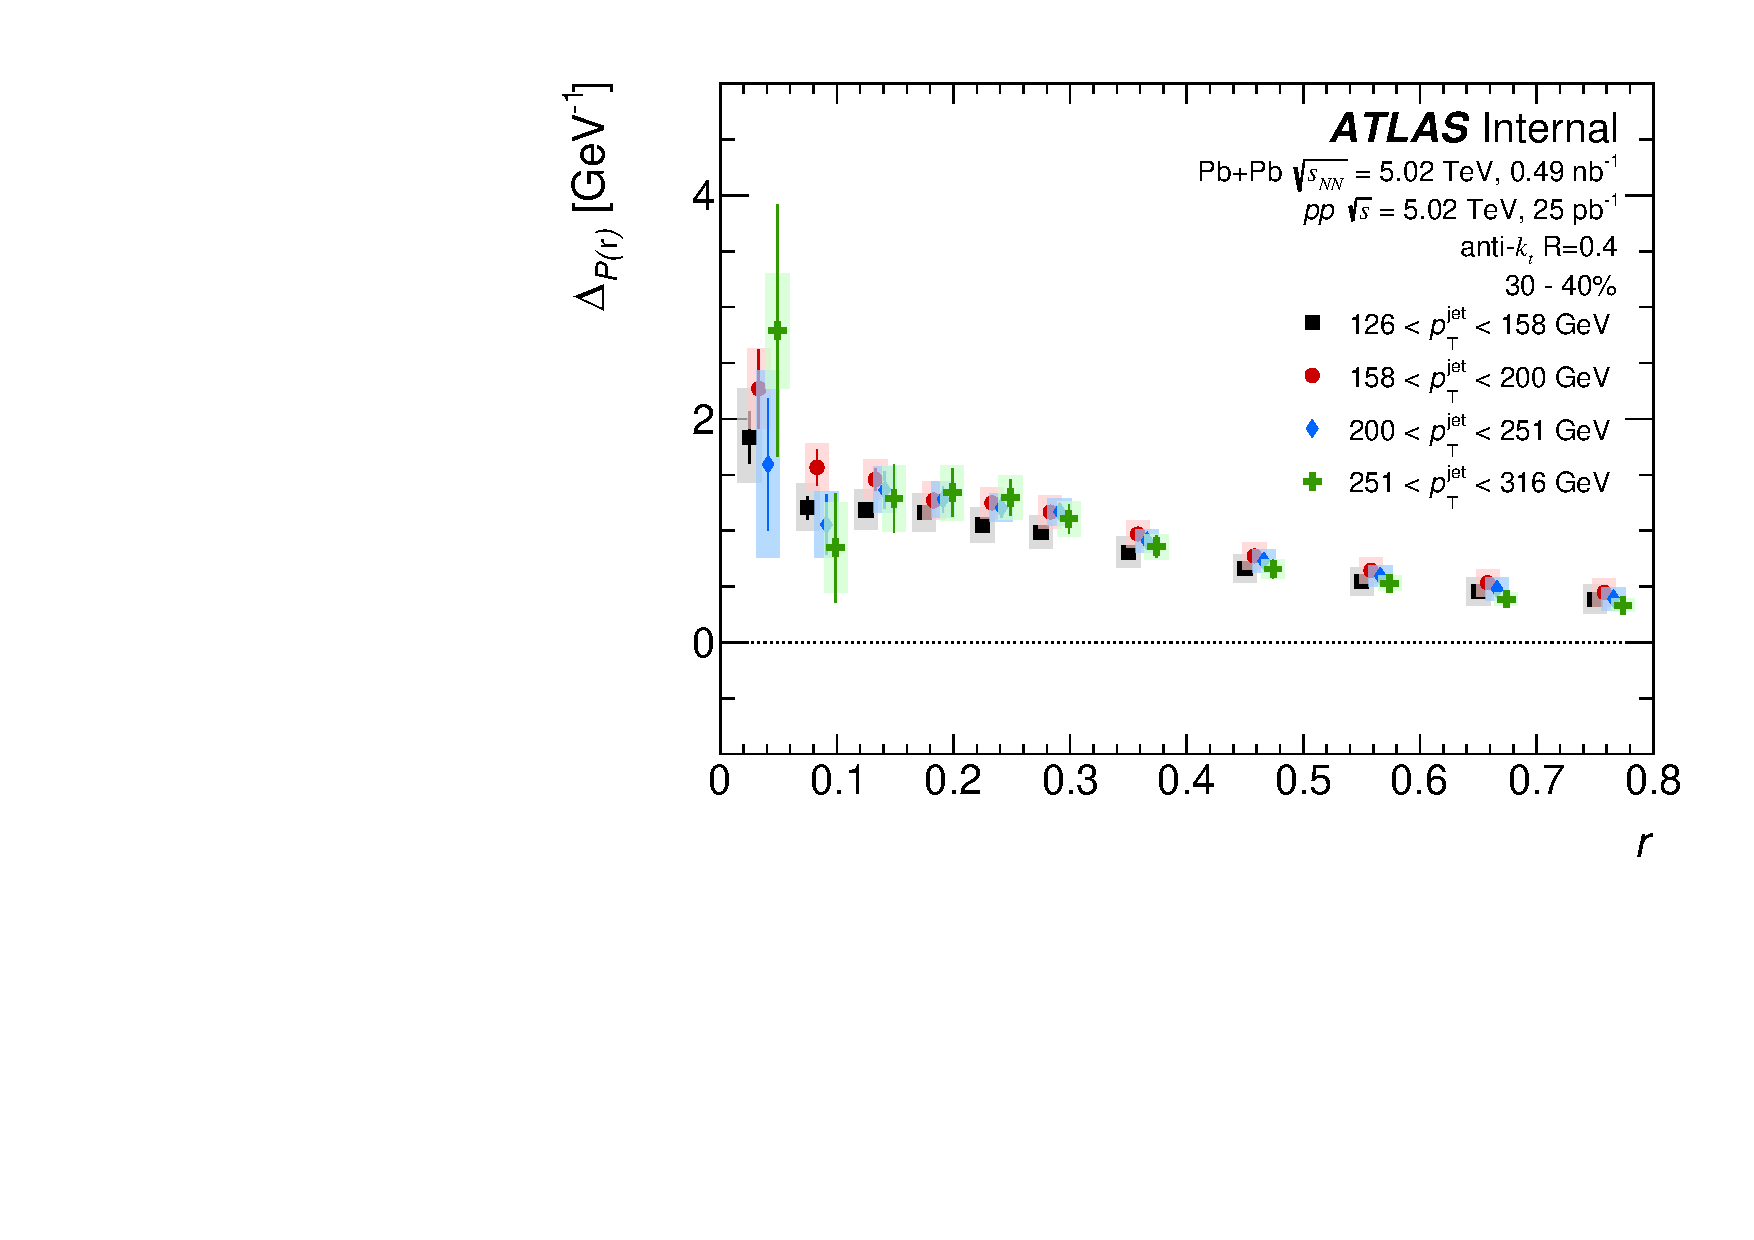
\includegraphics[width=0.5\textwidth]{results/DeltaDpT_jetshape_cent3.pdf} \\
 	 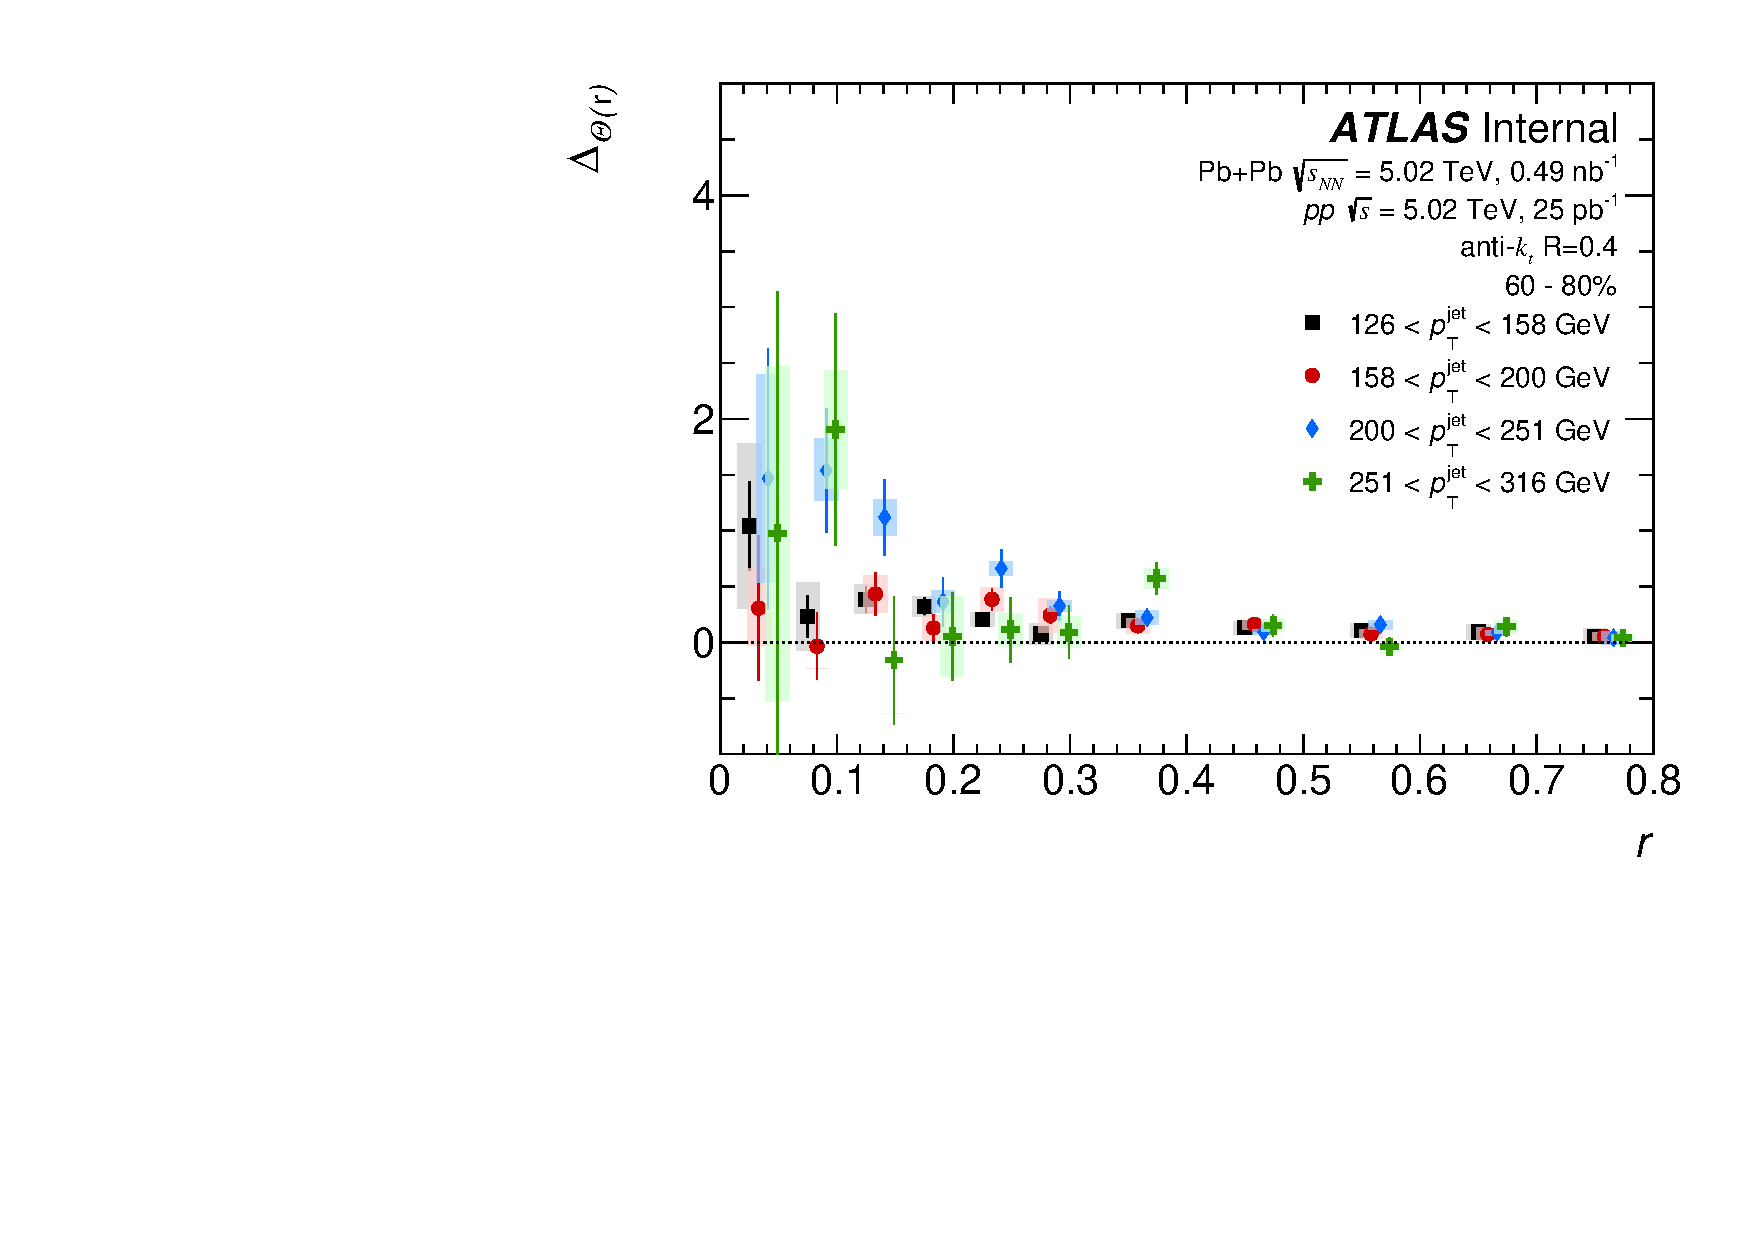
\includegraphics[width=0.48\textwidth]{results/DeltaDpT_lowpt_integ_cent5.pdf} 
%	 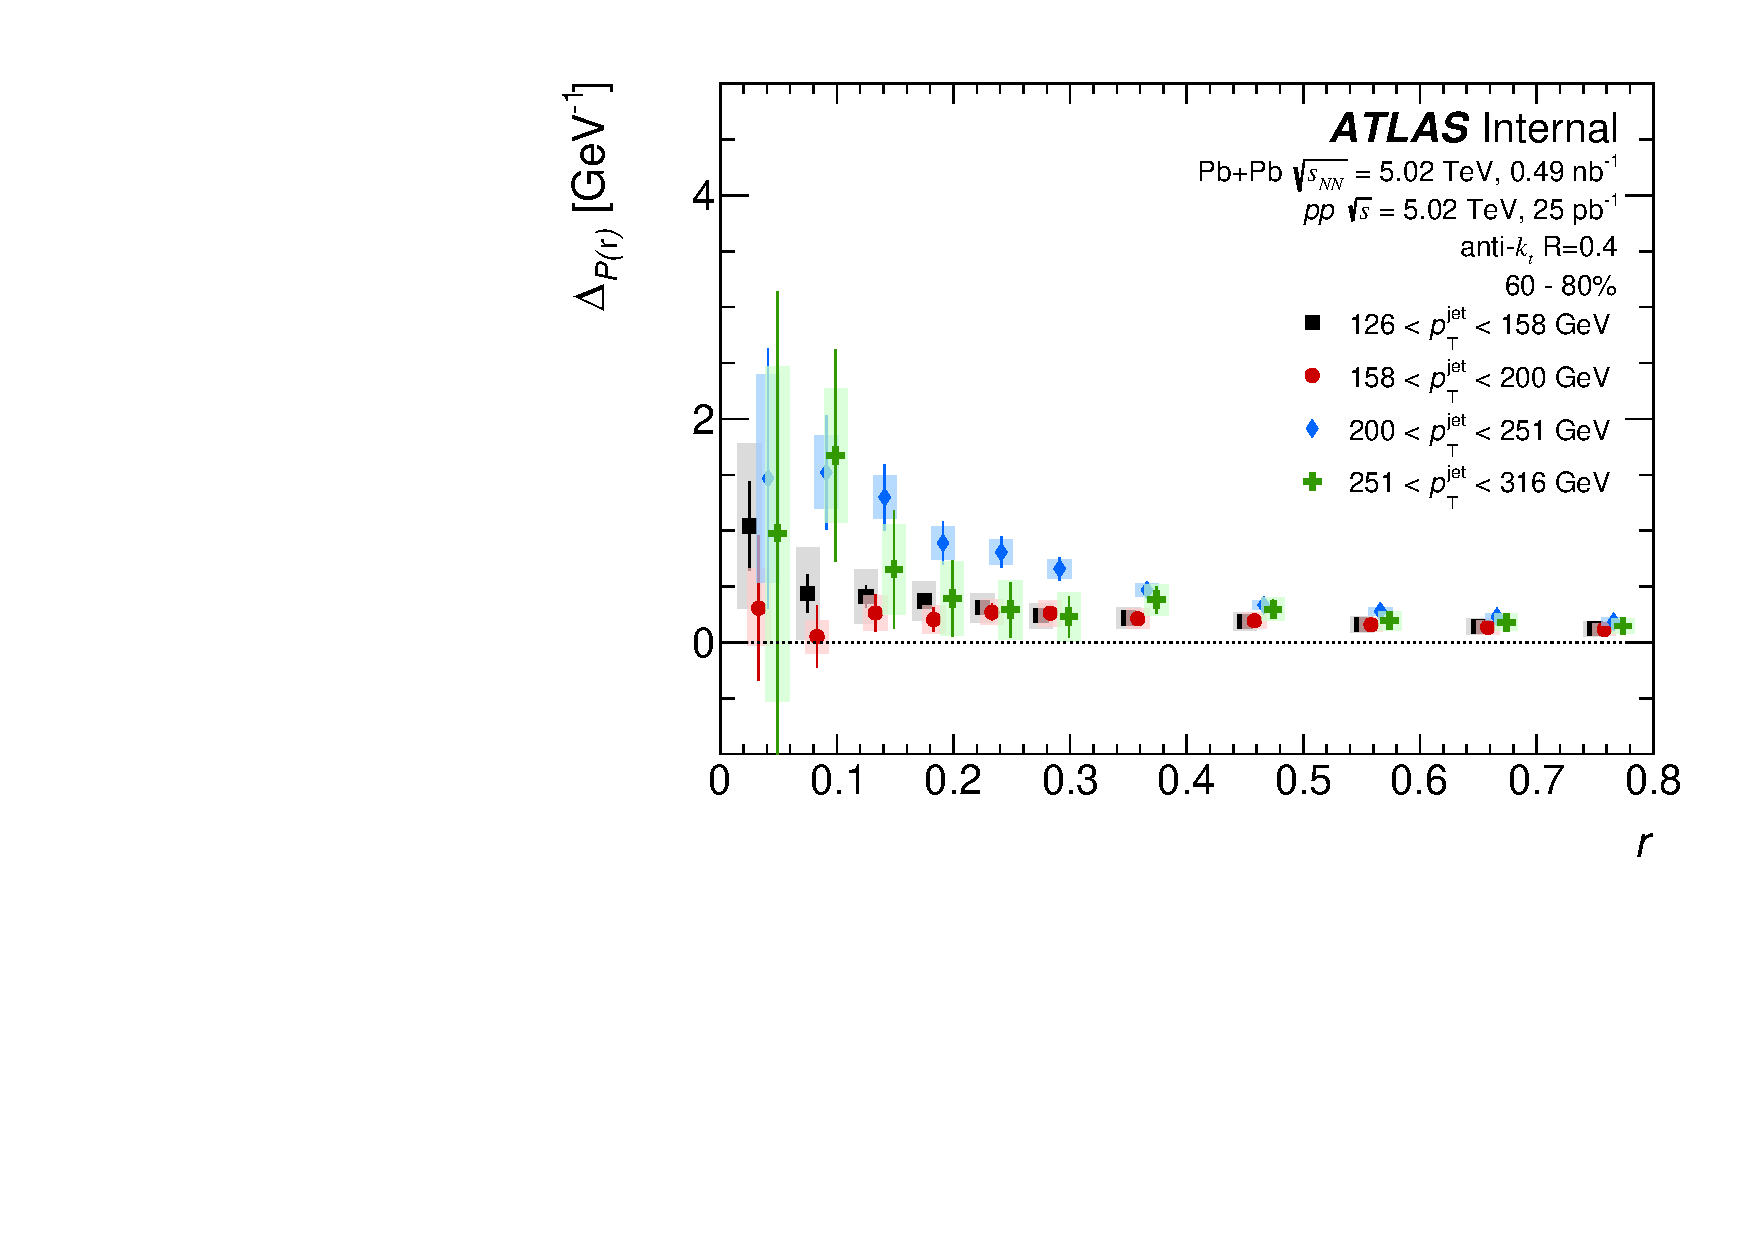
\includegraphics[width=0.5\textwidth]{results/DeltaDpT_jetshape_cent5.pdf} \\
\end{tabular} }
   \caption{\DeltaTheta\ as a function of \rvar\ for charged-particles with \pt\ < 4 GeV ranges in 
   four \ptjet\ selections: 126--158~\GeV, 158--200~\GeV, 200--251~\GeV, and 251--316~\GeV and three centrality 
   selections: 0--10\% (left), 30--40\% (middle) and 60--80\% (right). 
   The vertical bars on the data points indicate statistical uncertainties while the shaded boxes indicate systematic uncertainties. The widths of the boxes are not indicative of the bin size and the points are shifted horizontally for better visibility. }
      \label{fig:deltaPdeltaT}
\end{figure}


\begin{figure}
\centering{
\begin{tabular}{cc}
	 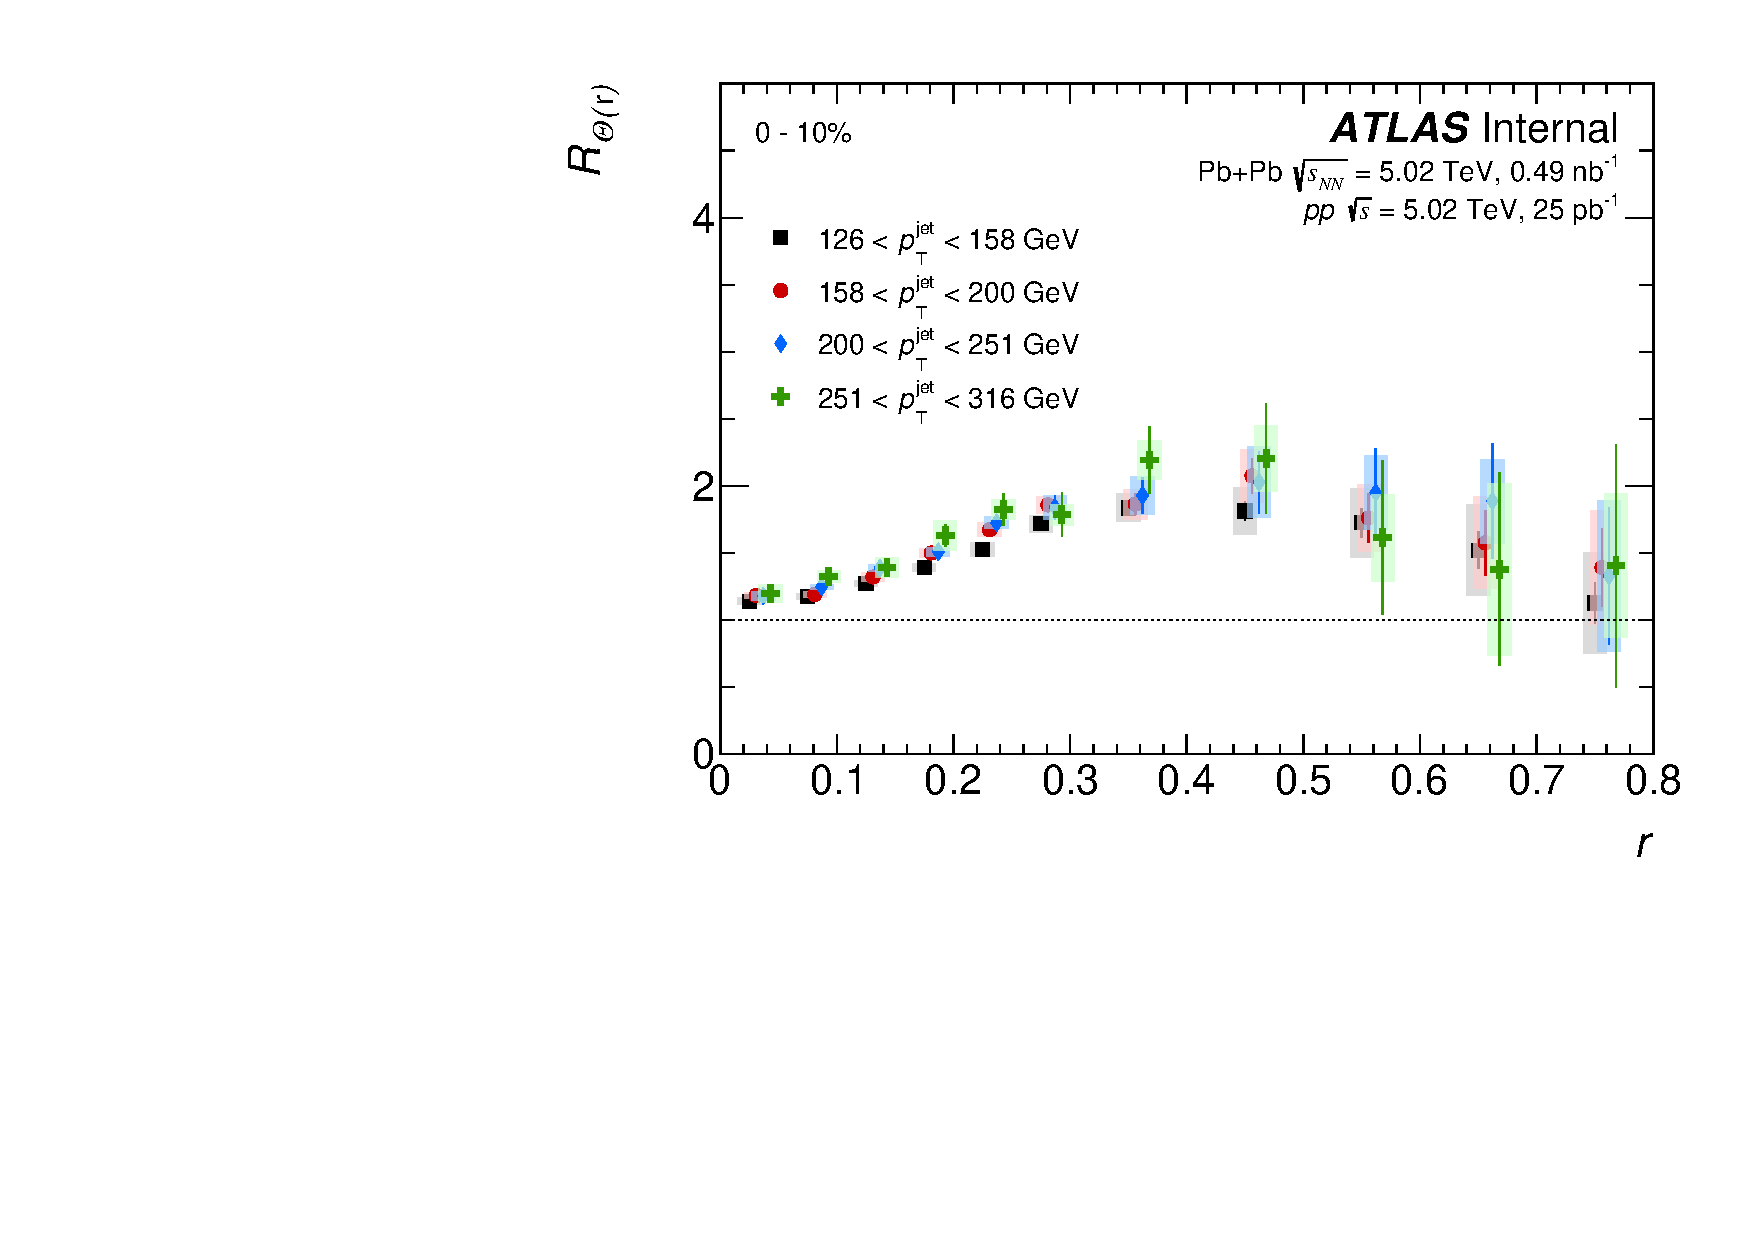
\includegraphics[width=0.5\textwidth]{results/RDpT_lowpt_integ_cent0.pdf} &
	 \includegraphics[width=0.5\textwidth]{results/RDpT_jetshape_cent0.pdf} \\
	 \includegraphics[width=0.5\textwidth]{results/RDpT_lowpt_integ_cent3.pdf} &
	 \includegraphics[width=0.5\textwidth]{results/RDpT_jetshape_cent3.pdf} \\
	 \includegraphics[width=0.5\textwidth]{results/RDpT_lowpt_integ_cent5.pdf} &
	 \includegraphics[width=0.5\textwidth]{results/RDpT_jetshape_cent5.pdf} \\
\end{tabular} }
   \caption{\RTheta\ (left) and \RP\ (right) as a function of \rvar\ in central collisions for charged-particles with $\pt < 4$ GeV ranges in four \ptjet\ selections: 126--158~\GeV, 158--200~\GeV, 200--251~\GeV, and 251--316~\GeV\ and three centrality selections: 0--10\% (top), 30--40\% (middle) and 60--80\% (bottom). The vertical bars on the data points indicate statistical uncertainties while the shaded boxes indicate systematic uncertainties. The widths of the boxes are not indicative of the bin size and the points are shifted horizontally for better visibility. }
      \label{fig:RPRT}
\end{figure}


Figure~\ref{fig:RPRT} shows \RTheta\ and \RP\ for 0--10\%, 30--40\% and 60--80\% central collisions.  The \RTheta\ 
distributions of the most central collisions show a maximum for $\rvar \sim 0.4$ and a flattening or a decrease for larger \rvar.
However, since \RTheta\ remains at or above unity for the full range of \rvar\ values presented \RP\ continues
to slowly increase with increasing \rvar\ over the full measured range.  In more peripheral collisions,
the magnitude of the excess is reduced and the trends in \RTheta\ are less clear, however the slow increase
of \RP\ is clearly seen for the 30--40\% central collisions.


%These measurements show that the excess of particles with $\pt <$~4.0~\GeV\ observed in~\cite{Aaboud:2018hpb} extends
%outside the \RFour\ jet cone.
%The measured dependence of \RDptr\ suggests that the energy lost by jets through the jet quenching process is being transferred to particles with $\pt <$~4.0~\GeV\ at larger radial distances from the jet axis. 
%This is qualitatively consistent with theoretical calculations \mbox{\cite{Blaizot:2014ula}}.
%Additionally, these observations are in agreement with the previous measurement of jet fragmentation functions \cite{Chatrchyan:2014ava, Sirunyan:2018jqr, Aaboud:2017bzv, Aaboud:2018hpb} and may indicate the dependence of the response of the hot dense matter to the momentum of a jet passing through it. 


\FloatBarrier

%-------------------------------------------------------------------------------
\section{Summary}
\label{sec:summary}
% !TEX root = trkjet.tex

This paper presents a measurement of the yields of charged particle distributions, \Dptr, inside and around \RFour\ \antikt\ jets with $|\yjet| <$1.7 up to a distance of $r = 0.8$ from the jet axis. The yields are measured in intervals of \ptjet\ from 126 to 316~\GeV\ in \PbPb\ and \pp\ collisions at 5.02~\TeV\ as a function of charged particle \pt\ and the angular distance \rvar\ between the jet axis and charged particle.

Centrality dependent modifications to the yields, when compared to those measured in \pp\ collisions, are observed. The magnitude of these modifications increases with increasing collision centrality. 
The \RDptr\ distributions for charged particles with $\pt <$~4~\GeV\ 
are above unity and 
grow with increasing angular separation up to $r \sim0.3$, showing weak to no dependence on $r$ in the interval 0.3~$< \rvar <$~0.6 followed with a small decrease in the enhancement for 0.6~$< \rvar <$~0.8.
For charged particles with $\pt >$~4~\GeV, a suppression in \RDptr\ is observed, and the 
distributions decrease with increasing
\rvar\ for $\rvar < $~0.3, with no \rvar\ dependence for $r>0.3$. 
These results show a broadening of the \Dptr\ distribution for low \pt\ particles inside the jet
in central \pbpb\ collisions compared to those in \pp\ collisions while for higher \pt\ particles
angular distributions are narrower in \pbpb\ collisions compared to \pp\ collisions.
For all charged-particle \pt\ values the \RDptr\ values are greater than or equal to unity for
small \rvar\ values (inside the core of the jet).
Between $0.1 < r < 0.25$, a statistically significant trend of increasing \RDptr\ with increasing \ptjet\ is observed for low-\pt\ particles. No significant \ptjet\ dependence is seen for particles  with $\pt >$~4~\GeV.

These measurements provide insight into the differential distributions of charged particles within jets as compared to the inclusive measurement of jet fragmentation functions. % and are important
%for understanding how jets interact with the QGP.
They provide new information about our understanding of the physics of soft
gluon radiation and the response of the QGP to jets.

%-------------------------------------------------------------------------------
\section*{Acknowledgements}
% Acknowledgements for papers with collision data
% Version 24-Oct-2018

% Standard acknowledgements start here
%----------------------------------------------
We thank CERN for the very successful operation of the LHC, as well as the
support staff from our institutions without whom ATLAS could not be
operated efficiently.

We acknowledge the support of ANPCyT, Argentina; YerPhI, Armenia; ARC, Australia; BMWFW and FWF, Austria; ANAS, Azerbaijan; SSTC, Belarus; CNPq and FAPESP, Brazil; NSERC, NRC and CFI, Canada; CERN; CONICYT, Chile; CAS, MOST and NSFC, China; COLCIENCIAS, Colombia; MSMT CR, MPO CR and VSC CR, Czech Republic; DNRF and DNSRC, Denmark; IN2P3-CNRS, CEA-DRF/IRFU, France; SRNSFG, Georgia; BMBF, HGF, and MPG, Germany; GSRT, Greece; RGC, Hong Kong SAR, China; ISF and Benoziyo Center, Israel; INFN, Italy; MEXT and JSPS, Japan; CNRST, Morocco; NWO, Netherlands; RCN, Norway; MNiSW and NCN, Poland; FCT, Portugal; MNE/IFA, Romania; MES of Russia and NRC KI, Russian Federation; JINR; MESTD, Serbia; MSSR, Slovakia; ARRS and MIZ\v{S}, Slovenia; DST/NRF, South Africa; MINECO, Spain; SRC and Wallenberg Foundation, Sweden; SERI, SNSF and Cantons of Bern and Geneva, Switzerland; MOST, Taiwan; TAEK, Turkey; STFC, United Kingdom; DOE and NSF, United States of America. In addition, individual groups and members have received support from BCKDF, CANARIE, CRC and Compute Canada, Canada; COST, ERC, ERDF, Horizon 2020, and Marie Sk{\l}odowska-Curie Actions, European Union; Investissements d' Avenir Labex and Idex, ANR, France; DFG and AvH Foundation, Germany; Herakleitos, Thales and Aristeia programmes co-financed by EU-ESF and the Greek NSRF, Greece; BSF-NSF and GIF, Israel; CERCA Programme Generalitat de Catalunya, Spain; The Royal Society and Leverhulme Trust, United Kingdom. 

The crucial computing support from all WLCG partners is acknowledged gratefully, in particular from CERN, the ATLAS Tier-1 facilities at TRIUMF (Canada), NDGF (Denmark, Norway, Sweden), CC-IN2P3 (France), KIT/GridKA (Germany), INFN-CNAF (Italy), NL-T1 (Netherlands), PIC (Spain), ASGC (Taiwan), RAL (UK) and BNL (USA), the Tier-2 facilities worldwide and large non-WLCG resource providers. Major contributors of computing resources are listed in Ref.~\cite{ATL-GEN-PUB-2016-002}.
%----------------------------------------------


%-------------------------------------------------------------------------------

% All figures and tables should appear before the summary and conclusion.
% The package placeins provides the macro \FloatBarrier to achieve this.
% \FloatBarrier


%The \texttt{atlaslatex} package contains the acknowledgements that were valid 
%at the time of the release you are using.
%These can be found in the \texttt{acknowledgements} subdirectory.
%When your ATLAS paper or PUB/CONF note is ready to be published,
%download the latest set of acknowledgements from:\\
%\url{https://twiki.cern.ch/twiki/bin/view/AtlasProtected/PubComAcknowledgements}


%-------------------------------------------------------------------------------
%\clearpage
%\appendix
%\part*{Appendix}
%\addcontentsline{toc}{part}{Appendix}
%-------------------------------------------------------------------------------


%-------------------------------------------------------------------------------
% If you use biblatex and either biber or bibtex to process the bibliography
% just say \printbibliography here
\printbibliography
% If you want to use the traditional BibTeX you need to use the syntax below.
% \bibliographystyle{obsolete/bst/atlasBibStyleWoTitle}
% \bibliography{trkjet,bib/ATLAS,bib/CMS,bib/ConfNotes,bib/PubNotes}
%-------------------------------------------------------------------------------

%-------------------------------------------------------------------------------
% Author list - comment in this line when you are ready to include it
% \clearpage
% \input{atlas_authlist}
%-------------------------------------------------------------------------------

%-------------------------------------------------------------------------------
% Auxiliary material - comment out the following line if you do not have any
% !TEX root = trkjet.tex

\part*{Auxiliary material}
\addcontentsline{toc}{part}{Auxiliary material}
%-------------------------------------------------------------------------------

%In an ATLAS paper, auxiliary plots and tables that are supposed to be made public 
%should be collected in an appendix that has the title \enquote{Auxiliary material}.
%This information will appear on the public webpage, but will not be included
%in the document submitted to arXiv and to the journal.

%
%\begin{figure}[h]
%\includegraphics[width=1.0\textwidth]{figures/results/DpT_dR_jet7}
%\caption{ \Dptr\ distributions as a function of \rvar\ for different \pt\ ranges in 126--158 GeV jets.
%The open markers are for \pp\ collisions and the solid markers are for \pbpb\ collisions.
%The different panels refer to different centrality selections}
%\label{fig:fullset_dptr_j7}
%\end{figure}

\begin{figure}[h]
\centerline{
\begin{tabular}{ccc}
\includegraphics[width=0.48\textwidth]{figures/results/DpT_dR_jet8_cent0} &
\includegraphics[width=0.48\textwidth]{figures/results/DpT_dR_jet8_cent1} \\
\includegraphics[width=0.48\textwidth]{figures/results/DpT_dR_jet8_cent2} &
\includegraphics[width=0.48\textwidth]{figures/results/DpT_dR_jet8_cent3} \\
\includegraphics[width=0.48\textwidth]{figures/results/DpT_dR_jet8_cent4} &
\includegraphics[width=0.48\textwidth]{figures/results/DpT_dR_jet8_cent5} \\
\end{tabular}}
\caption{ \Dptr\ distributions as a function of \rvar\ for different \pt\ ranges in 158--200 GeV jets.
The open markers are for \pp\ collisions and the solid markers are for \pbpb\ collisions.
The different panels refer to different centrality selections.
The vertical bars on the data points indicate statistical uncertainties while the shaded boxes indicate systematic uncertainties.
The widths of the boxes are not indicative of the bin size and the points are shifted horizontally for better visibility.
The distributions for $\pt > 6.3$ GeV are restricted to smaller \rvar\ values as discussed in Section~\ref{sec:analysis}.}
\label{fig:fullset_dptr_j8}
\end{figure}

\begin{figure}[h]
\centerline{
\begin{tabular}{ccc}
\includegraphics[width=0.48\textwidth]{figures/results/DpT_dR_jet9_cent0} &
\includegraphics[width=0.48\textwidth]{figures/results/DpT_dR_jet9_cent1} \\
\includegraphics[width=0.48\textwidth]{figures/results/DpT_dR_jet9_cent2} &
\includegraphics[width=0.48\textwidth]{figures/results/DpT_dR_jet9_cent3} \\
\includegraphics[width=0.48\textwidth]{figures/results/DpT_dR_jet9_cent4} &
\includegraphics[width=0.48\textwidth]{figures/results/DpT_dR_jet9_cent5} \\
\end{tabular}}
\caption{ \Dptr\ distributions as a function of \rvar\ for different \pt\ ranges in 200--251 GeV jets.
The open markers are for \pp\ collisions and the solid markers are for \pbpb\ collisions.
The different panels refer to different centrality selections.
The vertical bars on the data points indicate statistical uncertainties while the shaded boxes indicate systematic uncertainties.
The widths of the boxes are not indicative of the bin size and the points are shifted horizontally for better visibility.
The distributions for $\pt > 6.3$ GeV are restricted to smaller \rvar\ values as discussed in Section~\ref{sec:analysis}.}
\label{fig:fullset_dptr_j9}
\end{figure}


\begin{figure}[h]
\centerline{
\begin{tabular}{ccc}
\includegraphics[width=0.48\textwidth]{figures/results/DpT_dR_jet10_cent0} &
\includegraphics[width=0.48\textwidth]{figures/results/DpT_dR_jet10_cent1} \\
\includegraphics[width=0.48\textwidth]{figures/results/DpT_dR_jet10_cent2} &
\includegraphics[width=0.48\textwidth]{figures/results/DpT_dR_jet10_cent3} \\
\includegraphics[width=0.48\textwidth]{figures/results/DpT_dR_jet10_cent4} &
\includegraphics[width=0.48\textwidth]{figures/results/DpT_dR_jet10_cent5} \\
\end{tabular}}
\caption{ \Dptr\ distributions as a function of \rvar\ for different \pt\ ranges in 251--316 GeV jets.
The open markers are for \pp\ collisions and the solid markers are for \pbpb\ collisions.
The different panels refer to different centrality selections.
The vertical bars on the data points indicate statistical uncertainties while the shaded boxes indicate systematic uncertainties.
The widths of the boxes are not indicative of the bin size and the points are shifted horizontally for better visibility.}
\label{fig:fullset_dptr_j10}
\end{figure}




\begin{figure}[h]
\centerline{
\begin{tabular}{ccc}
\includegraphics[width=0.48\textwidth]{figures/results/RDpT_dR_jet7_cent0} &
\includegraphics[width=0.48\textwidth]{figures/results/RDpT_dR_jet7_cent1} \\
\includegraphics[width=0.48\textwidth]{figures/results/RDpT_dR_jet7_cent2} &
\includegraphics[width=0.48\textwidth]{figures/results/RDpT_dR_jet7_cent3} \\
\includegraphics[width=0.48\textwidth]{figures/results/RDpT_dR_jet7_cent4} &
\includegraphics[width=0.48\textwidth]{figures/results/RDpT_dR_jet7_cent5} \\
\end{tabular}}
\caption{ The \RDptr\ distributions as a function of \rvar\ for different \pt\ selections in 126--158 GeV jets.
The different panels refer to different centrality selections.
The vertical bars on the data points indicate statistical uncertainties while the shaded boxes indicate systematic uncertainties.
The widths of the boxes are not indicative of the bin size and the points are shifted horizontally for better visibility.}
\label{fig:fullset_rptr_j7}
\end{figure}

\begin{figure}[h]
\centerline{
\begin{tabular}{ccc}
\includegraphics[width=0.48\textwidth]{figures/results/RDpT_dR_jet8_cent0} &
\includegraphics[width=0.48\textwidth]{figures/results/RDpT_dR_jet8_cent1} \\
\includegraphics[width=0.48\textwidth]{figures/results/RDpT_dR_jet8_cent2} &
\includegraphics[width=0.48\textwidth]{figures/results/RDpT_dR_jet8_cent3} \\
\includegraphics[width=0.48\textwidth]{figures/results/RDpT_dR_jet8_cent4} &
\includegraphics[width=0.48\textwidth]{figures/results/RDpT_dR_jet8_cent5} \\
\end{tabular}}
\caption{ The \RDptr\ distributions as a function of \rvar\ for different \pt\ selections in 158--200 GeV jets.
The different panels refer to different centrality selections.
The vertical bars on the data points indicate statistical uncertainties while the shaded boxes indicate systematic uncertainties.
The widths of the boxes are not indicative of the bin size and the points are shifted horizontally for better visibility.}
\label{fig:fullset_rptr_j7}
\end{figure}

\begin{figure}[h]
\centerline{
\begin{tabular}{ccc}
\includegraphics[width=0.48\textwidth]{figures/results/RDpT_dR_jet9_cent0} &
\includegraphics[width=0.48\textwidth]{figures/results/RDpT_dR_jet9_cent1} \\
\includegraphics[width=0.48\textwidth]{figures/results/RDpT_dR_jet9_cent2} &
\includegraphics[width=0.48\textwidth]{figures/results/RDpT_dR_jet9_cent3} \\
\includegraphics[width=0.48\textwidth]{figures/results/RDpT_dR_jet9_cent4} &
\includegraphics[width=0.48\textwidth]{figures/results/RDpT_dR_jet9_cent5} \\
\end{tabular}}
\caption{ The \RDptr\ distributions as a function of \rvar\ for different \pt\ selections in 200--251 GeV jets.
The different panels refer to different centrality selections.
The vertical bars on the data points indicate statistical uncertainties while the shaded boxes indicate systematic uncertainties.
The widths of the boxes are not indicative of the bin size and the points are shifted horizontally for better visibility.}
\label{fig:fullset_rptr_j7}
\end{figure}

\begin{figure}[h]
\centerline{
\begin{tabular}{ccc}
\includegraphics[width=0.48\textwidth]{figures/results/RDpT_dR_jet10_cent0} &
\includegraphics[width=0.48\textwidth]{figures/results/RDpT_dR_jet10_cent1} \\
\includegraphics[width=0.48\textwidth]{figures/results/RDpT_dR_jet10_cent2} &
\includegraphics[width=0.48\textwidth]{figures/results/RDpT_dR_jet10_cent3} \\
\includegraphics[width=0.48\textwidth]{figures/results/RDpT_dR_jet10_cent4} &
\includegraphics[width=0.48\textwidth]{figures/results/RDpT_dR_jet10_cent5} \\
\end{tabular}}
\caption{ The \RDptr\ distributions as a function of \rvar\ for different \pt\ selections in 251--316 GeV jets.
The different panels refer to different centrality selections.
The vertical bars on the data points indicate statistical uncertainties while the shaded boxes indicate systematic uncertainties.
The widths of the boxes are not indicative of the bin size and the points are shifted horizontally for better visibility.}
\label{fig:fullset_rptr_j7}
\end{figure}

%-------------------------------------------------------------------------------

%-------------------------------------------------------------------------------
% Extra tables etc. for HepData - comment in the following line if you have any
% \section{HepData material}
%-------------------------------------------------------------------------------

This file is available for detailed tables etc.\ that are going to be
submitted to HepData or other similar destinations.

%-------------------------------------------------------------------------------

\end{document}
